% !TEX TS-program = pdflatex
% !TEX encoding = UTF-8 Unicode

%\documentclass[a4paper,twoside]{article}%                                        use larger type; default would be 10pt
\documentclass[a4paper]{article}%                                                 use larger type; default would be 10pt
\usepackage[utf8]{inputenc}%                                                      set input encoding (not needed with XeLaTeX)

%%% PAGE DIMENSIONS ------------------------------------------------------------
\usepackage{geometry}%              to change the page dimensions
\geometry{a4paper}%                                                               or letterpaper (US) or a5paper or....
\usepackage[parfill]{parskip}%                                                    Activate to begin paragraphs with an empty line rather than an indent

%%% HEADERS & FOOTERS ----------------------------------------------------------
\usepackage{fancyhdr}%                                                            This should be set AFTER setting up the page geometry
\pagestyle{fancy}%                                                                options: empty , plain , fancy
\renewcommand{\headrulewidth}{0pt}%                                               customise the layout...
\lhead{}\chead{}\rhead{}
\lfoot{}\cfoot{page \thepage}\rfoot{}

%%% SECTION TITLE APPEARANCE ---------------------------------------------------
\usepackage{sectsty}
\allsectionsfont{\sffamily\mdseries\upshape}%                                     (See the fntguide.pdf for font help)

%%% PACKAGES -------------------------------------------------------------------
\usepackage{morefloats}
\usepackage[font=small,labelfont=bf,textfont=it]{caption}%                        stylize captions
\usepackage[pdftex]{graphicx}%                                                    support the \includegraphics command and options
\usepackage{booktabs}%                                                            for much better looking tables
\usepackage{array}%                                                               for better arrays (eg matrices) in maths
\usepackage{paralist}%                                                            very flexible & customisable lists (eg. enumerate/itemize, etc.)
\usepackage{verbatim}%                                                            adds environment for commenting out blocks of text & for better verbatim
\usepackage{subfig}%                                                              make it possible to include more than one captioned figure/table in a single float
\usepackage{mathtools}%                                                           for math environments like align
\usepackage{amssymb}%                                                             for symbols like \therefore
\usepackage{verbatim}%                                                            for including text as appears, verbatim
\usepackage{listings}%                                                            for including external files as text, eg code
\usepackage{color}%                                                               for coloring of files and images
\usepackage{overpic}%                                                             for adding annotations to pictures
\usepackage[alsoload=astro]{siunitx}%                                                             for units \SI{}{}, \si{}, \num{} etc.
\usepackage{multirow}%                                                            for multiple row spanning cells in tables
\usepackage{rotating}%                                                            for the \begin{sideways} environment for sideways text

%%% EQUATIONS ------------------------------------------------------------------
\numberwithin{equation}{section}%                                                 Number equations by section (change for different levels)
	\DeclareSIUnit\pixel{pix}
	\DeclareSIUnit\ADU{ADU}
    \DeclareSIUnit\electron{\text{e}^{-{}}}
	\DeclareSIUnit\erg{erg}
    \DeclareSIUnit\year{yr}
    \DeclareSIUnit\omega{$\Omega$}

%% BIBIOGRAPHY ------------------------------------------------------------------
\usepackage{cite}

%%% ToC (table of contents) APPEARANCE -----------------------------------------
%\usepackage[nottoc,notlof,notlot]{tocbibind}                                   % Put the bibliography in the ToC
%\usepackage[titles,subfigure]{tocloft}                                         % Alter the style of the Table of Contents
%\renewcommand{\cftsecfont}{\rmfamily\mdseries\upshape}
%\renewcommand{\cftsecpagefont}{\rmfamily\mdseries\upshape}                     % No bold!
\setcounter{tocdepth}{2}

%%% PDF LINKS AND STYLE --------------------------------------------------------
\usepackage[unicode=true,
    bookmarks=true,bookmarksnumbered=true,bookmarksopen=true,
    bookmarksopenlevel=2, breaklinks=false,pdfborder={0 0 0},backref=false,
    colorlinks=false] {hyperref}%                                                 for links in pdf file, no colors
\hypersetup{pdftitle={Cosmic Re-ionisation},
    pdfauthor={Extragalactic Astrophysics and Cosmology Group Studies}}%		  set name of document and author here

%%% END Article customizations

%%% NEW COMMANDS ---------------------------------------------------------------
\renewcommand{\d}{\,\mathrm{d}}%                                                  for integrals
\newcommand{\dx}[2]{\frac{\textrm{d}#1}{\textrm{d}#2}}%                           for derivatives
\newcommand{\dd}[2]{\frac{\textrm{d}^2#1}{\textrm{d}#2^2}}%                       for double derivatives
\newcommand{\pd}[2]{\frac{\partial#1}{\partial#2}}%                               for partial derivatives
\newcommand{\pdd}[2]{\frac{\partial^2#1}{\partial#2^2}}%                          for double partial derivatives
\newcommand{\e}[1]{\text{e}^{#1}}%                                                for exponentials
\newcommand{\code}[1]{\texttt{#1}}%                                               for verbatim code view
\newcommand{\inter}[1]{\shortintertext{#1}}%                                      shorter version of intertext
\newcommand{\under}[1]{\underline{#1}}%                                           for vectors etc.

\let\vaccent=\v{}%                                                                rename builtin command \v{} to \vaccent{}
\newcommand{\uv}[1]{\ensuremath{\hat{#1}}}%                                       for unit vector
\newcommand{\abs}[1]{\left|#1\right|}%                                            for absolute value
\newcommand{\avg}[1]{\left<#1\right>}%                                            for average
\let\underdot=\d%                                                                 rename builtin command \d{} to \underdot{}
\newcommand{\ket}[1]{\left|#1\right>}%                                            for Dirac bras
\newcommand{\bra}[1]{\left<#1\right|}%                                            for Dirac kets
\newcommand{\braket}[2]{\left<#1\vphantom{#2} \right|
    \left.#2 \vphantom{#1} \right>}%                                              for Dirac brackets
\newcommand{\matrixel}[3]{\left<#1\vphantom{#2#3} \right|
    #2 \left|#3 \vphantom{#1#2}\right>}%                                          for Dirac matrix elements
\newcommand{\grad}[1]{\nabla#1}%                                                  for gradient
\let\divsymb=\div%                                                                rename builtin command \div to \divsymb
\renewcommand{\div}[1]{\nabla\cdot#1}%                                            for divergence
\newcommand{\curl}[1]{\nabla\times#1}%                                            for curl
\let\baraccent=\={}%                                                              rename builtin command \= to \baraccent
\renewcommand{\=}[1]{\stackrel{#1}{=}}%                                           for putting numbers above =

\newcolumntype{L}{>{\centering\arraybackslash}m{3em}}

%*******************************************************************************
%******************************** END HEADER ***********************************
%*******************************************************************************

\begin{document}
%!TEX root = mainfile.tex
\begin{titlepage}
  \begin{center}
    \vspace*{\fill}

    \centering
    
\includegraphics[scale=1.0]{Logo.pdf}
    \vfill

    \hrule
    {\LARGE\bf Extragalactic Astrophysics and Cosmology\\Cosmic Reionization \\[0.4cm]}
    \hrule

    \vfill
    \large
    School of Physics and Astronomy\\
    University of Birmingham

    \vfill
    { Joe Baumber,
    	James Bryant,
    	Lewis Clegg,
    	Bethany Johnson,
    	Andrew King,
    	Owen McConnell,
    	Catherine McDonald,
    	Michael O'Neill,
    	Jonathan Shepley,
    	Dorothy Stonell,
    	Rahim Topadar,
    	Josh Wainwright\\}
    \vfill

    \vfill
    \textit{Supervisors:} Graham Smith, Alistair Sanderson, Melissa Gillone \\
    		\vfill
    \textit{Date:} March 2013
    \vfill
    \vfill

    \begin{abstract}
        This study deduces that reionization began at a redshift of $z=17.82$ and ended at a redshift of $z=7\pm 1.8$. This is calculated by directly applying the dynamics of star formation and the ionization rate of neutral hydrogen in the Intergalactic Medium. A photometry strategy consisting of 3 multi-band surveys is proposed in order to observe Lyman Break Galaxies across redshifts 6--17. The surveys will locate $100.5\pm37.0$, $138.7\pm 100.6$, $358.1\pm 158.6$ galaxies in redshift ranges 6--8.5, 8.5--10 and 10--17 respectively. These surveys will be completed by the James Webb Space Telescope and Euclid which are planned for launch in the coming decade. A follow up spectroscopy survey will be used to confirm the redshift and properties of 24, 4 and 48 galaxies in these 3 surveys respectively. The spectroscopy will be carried out using James Webb Space Telescope and a combination of single and multi-slit spectroscopy. It is shown that the use of known gravitational lenses, located between redshift 0.5--0.7, is very beneficial for discovering high redshift candidates as it can increase the depth of surveys by up to 3 magnitudes.
    \end{abstract}


  \end{center}
\end{titlepage}

%\thispagestyle{empty}
%\vspace*{\fill}
%\noindent
%\begin{tabular}{ll}
%\end{tabular}

%\cleardoublepage
%\cleardoublepage

\newpage
\tableofcontents
\addcontentsline{toc}{section}{Contents}
% \listoffigures
% \listoftables
\newpage

\pagestyle{headings}
    %!TEX root = mainfile.tex

\section{Introduction} %fold
\label{section:Introduction}
	The evolution of the Universe has been divided up by cosmologists into several epochs; each characterised by their unique physical properties. This project focuses on the Epoch of Re-ionization (EoR) whereby high energy photons produced during active star formation ionized the neutral hydrogen in the Inter-Galactic Medium (IGM). In order to probe this particular era and learn more about it, early (high redshift) galaxies are being studied as it is believed that they produced these first ionizing photons and hence their birth should understandably correlate directly to the beginning of the Epoch of Cosmic Re-ionization. (more detail in section~\ref{sec:cosmic_re_ionisation}).

	There are many unanswered questions in cosmology; one of the most crucial is the nature of dark energy and matter which make up around 95\% of the universe\cite{WMAP9}. These mysterious substances are thought to be the key driving force behind the evolution and expansion of the universe. By studying and mapping the distribution of Hydrogen during the EoR and tracking the evolution of stars and galaxies we are able to infer more about the effects of dark energy and what it might consist of. There are many different theories about what dark matter consist of; the current most popular theories fall under the ``Cold Dark Matter'' model where dwarf galaxies are thought to be key building blocks in the hierarchical structure formation of the first galaxies\cite{Cignoni}.

	The process of Cosmic Re-ionization is crucial to our understanding of the evolution of the Universe as it forms the bridge between our present and a distant, ill-understood past. It links our current familiar universe whereby stars and galaxies are more common than the grains of sand on Earth's beaches to its past; when the Universe was a barren soup of free particles devoid of structure and life as we know it. Understanding the mechanisms of structure formation and what drives the collapse and formation of structure is fundamental in refining the Concordance Cosmology Model. Completing the picture of what happened during the EoR will enable us to more accurately predict where the Universe is headed and how it may eventually end, will it be in a ``big crunch'' or a ``big freeze''?

	The light from this era is so far away, and hence dim, that technology is only just allowing astronomers to see these early galaxies using high-powered telescopes and sophisticated detection process. There are a number of different projects in progress investigating this particular period of the universe and there are many more in the pipeline, these will be discussed in more detail in part~\ref{prt:observations}.

    \subsection{Structure of Study} %fold
    \label{Structure_of_Study}
		This study aims to develop an observing strategy based on original calculations for galaxy distributions and ultimately estimate the redshift range over which the EoR occurred. The group is split into two subgroups; a predictions group and an observational strategy group. The principal aim of the predictions group is to produce a set of calculations yielding the number of galaxies within the appropriate range of redshifts for re-ionization, with the inclusion of influences such as cosmic variance which skew the distribution. By considering the star formation rates and the ionization rate of neutral hydrogen the upper and lower bounds of this range respectively is determined. The final observing strategy explores which facilities to use; both current and planned and any adjustments required. The plan calculates the amount of observing time required to identify and confirm the properties of galaxies during the EoR. It also considers how to limit objects which will spoil our results; contaminants such as foreground stars and Supernovae events. The strategy aims to see further than previously achieved in this field and help to drive the understanding of re-ionization to new heights.
	%subsection Structure_of_Study (end)
%section Introduction (end)

\newpage

\part{General Theory} % (fold)
\label{prt:general_theory}
    %!TEX root = mainfile.tex

\section{Cosmic Re-Ionization} % (fold)
\label{sec:cosmic_re_ionisation}
	It is now universally accepted that the Universe began with the Big Bang whereby matter erupted from a singularity in an unexplained burst of energy. Following this the Universe was so hot (approximately $10^{12}$--$10^{15}$\,\si{\kelvin}\cite{liddle2003introduction}) that the photons had enough energy to suppress the binding of nucleons and so the Universe remained a soup of free baryons, leptons and energetic photons (amongst other things) until just a few minutes after the Big Bang during the Epoch of Nucleosynthesis when the protons and neutrons could begin to form atomic nuclei. Approximately \num{300000} years after the Big Bang came the Epoch of Decoupling when the majority of photons had lost a large proportion of their energy from frequent collisions within the plasma and hence most were left with less than the minimum hydrogen ionization energy of \SI{13.6}{\electronvolt}\cite{liddle2003introduction}. This allowed the electrons to finally bind to the hydrogen nuclei to form neutral hydrogen atoms, free from interfering photons. These newly retired photons were now able to travel across the Universe. With the photons having too little energy to interact with matter the Universe had become a transparent highway to our present and the photons set out on a journey which lasted almost as long as the age of the Universe, eventually arriving at Earth as a blanket of radiation known as the Cosmic Microwave Background.

	Meanwhile, in the wake of Decoupling matter was able to interact without disturbance from photons; atomically and gravitationally. Small density fluctuations, seen from Earth as small temperature fluctuations in the Cosmic Microwave Background, began to grow to such an extent that their gravity became large enough to attract matter, as more and more matter was attracted the gravitation became stronger and hence attracted more matter. This was the beginning of structure formation and the era known as ``Cosmic Re-ionization''. As more and more matter accumulated, stars began to form with high enough core temperatures to create photons with enough energy to once again ionize the neutral hydrogen in the IGM. As more stars formed, more of these high energy photons were being produced; gradually transforming the dark, neutral Universe to its current ionized state.

	In order for these photons to ionize the IGM, they evidently must reach it and hence must escape from their resident galaxy. The rate at which these photons were produced and escaped determines the length of time over which re-ionization occurred if one defines the end of re-ionization as being the point at which all, or at least the vast majority, of neutral hydrogen has been ionized. This requires one to understand how these early galaxies formed and thus infer their characteristic temperatures to see how many photons may have had enough energy to fully ionize the neutral hydrogen. Then one must consider what fraction of these photons could escape from the galaxy having managed to avoid interactions with the dust and neutral hydrogen within it. The specifics of this topic will be covered in more detail in Section~\ref{sec:determining_the_rate_of_re_ionizing_photons}.
% section cosmic_re_ionisation (end)

    \newpage
    %!TEX root = mainfile.tex

\section{Gravitational Lensing} % (fold)
\label{sec:gravitational_lensing}

	\subsection{Introduction} % (fold)
	\label{sub:introduction}
		Contrary to a popularly held belief that it was Newton who first referred to gravitational lensing in his publication ``Opticks''\cite{Newton_Opticks} (put into context, it is clear that he was discussing diffraction), the first person to allude directly to the bending of light due to gravitational attraction was Henry Cavendish. Around the turn of the 19th century Cavendish used Newton's corpuscular theory to correctly calculate the bending of light around a massive object.  Around the same time, German astronomer Johann Soldner was independently addressing the same problem\cite{Soldner} and although his results were similar to those obtained by Cavendish, his method was fundamentally flawed due to incorrect assumptions\cite{Conceptual_origins_of_GL}.

		The subject of gravitational lensing was then largely put to rest until 1915 when Einstein postulated his theory of General Relativity, from which it is clear that massive objects will cause light to bend as a result of the curvature of spacetime. Despite having complete and correct calculations of the phenomenon of gravitational lensing, including the lens equation and the position of images, Einstein displayed very little interest in it. He mentions it only briefly in his notebooks and published a single, very short discussion in Science Magazine upon the request of a friend at the end of which he dismissively comments that there is ``no great chance of this phenomenon being observed''\cite{Einstein_science_magazine}.

		During a solar eclipse in 1919, Eddington measured the positions of stars lying close to the Sun and observed that their positions appeared at a greater distance from the Sun than expected, thereby giving the first experimental evidence for the bending of light around the Sun\cite{Eddington_GL_evidence}. 5 years later, Chwolson published a paper on the idea that `fake double stars' may be observed as a result of the gravitational lensing effect and postulated that if source, lens and observer are perfectly aligned then a `Chwolson ring', later renamed ``Einstein ring'', would form around the lens\cite{Conceptual_origins_of_GL}.

		The true pioneer of the subject, however, is generally considered to be Czech astronomer\cite{F_Link_GL} Frantisek Link. Through detailed calculations of image magnification and positions, Link concluded that in some cases gravitational lensing would make faint sources visible. Optimistic about the possibility of observing these sources, particularly for spiral nebulae, he published a detailed paper on his wide ranging calculations which included the deflection undergone by light rays passing massive objects, the resulting change in intensity of sources and the invariance of source surface brightness. Following this, there was again a period of lack of interest, during which only a few papers were published on the subject until the discovery of the first lens in 1979 by Walsh, Carswell and Weymann. From here onwards, it became a topic of intense interest to astronomers and many more lenses and faint sources have since been discovered\cite{Conceptual_origins_of_GL}.
	% subsection introduction (end)

	\subsection{Concept} % (fold)
	\label{sub:concept}
		The bending of light around a massive object is a direct result of Einstein's theory of relativity and the curvature of spacetime. This effect can cause massive objects to act as lenses for background sources by bending the light such that rays that otherwise would not have been detected converge at the observer, resulting in a brighter image being observed. The increase in flux reaching the observer can result in significant magnification of a source, for example, one of the most distant objects known was observed behind the cluster Abell 2218 with a magnification factor of 30, equivalent to a decrease of 3.7 AB magnitudes\cite{Distant_object_Abell2218}. Studying the magnification and properties of the images can yield information about both the lens and the source, making it an extremely useful tool\cite{Hartle}.
		\begin{figure}[!htbp]
			\centering
				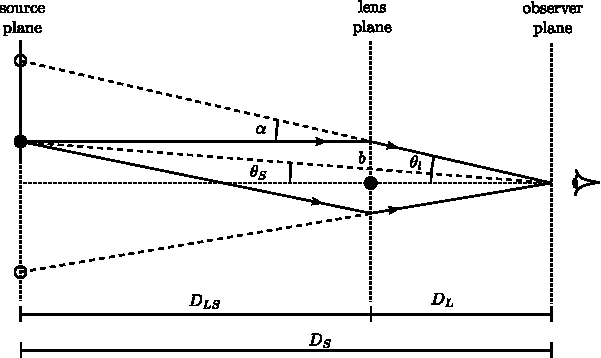
\includegraphics[width=0.6\textwidth]{../Images/Lensing_light_bending.pdf}
			\caption[Diagram of a gravitational lens]{In this schematic diagram of a gravitational lens, DL, DS and DLS represent the observer-lens, observer-source and lens-source distances respectively. $\theta_i$ is the image angle and $\theta_S$ the source angle, relative to the observer-lens axis. The light ray (solid line) passes by the lens at impact parameter $b$ and as a result is deflected by angle $\alpha$, converging with a second ray at the observer. The dotted lines indicate the position at which the images are observed\cite{Lensing_light_bending_diagram}.\label{fig:Lensing_light_bending}}
		\end{figure}

		The schematic diagram in Figure~\ref{fig:Lensing_light_bending} shows a gravitational lens acting on light from a background source in such a way as to form two images. The distances between observer, lens and source are so large in comparison to the impact parameter $b$ that to good approximation, the lens radius is negligible and it can be modelled as a thin lens. It is therefore reasonable to assume that the light travels in straight lines at all times except in the lens plane where the complete deflection occurs. Furthermore, it can be assumed that for all values of $b$, the deflection angle is given by
		\begin{align}
			\alpha &= \frac{4GM}{c^2 b}
		\end{align}
		where $M$ is the mass of the lens, c the speed of light and $G$ is the gravitational constant. In realistic lensing situations, all the angles shown in Figure~\ref{fig:Lensing_light_bending} are very small, hence the small angle approximation can be applied to yield the lens equation
		\begin{align}
			\theta_i D_S &= \theta_S D_S + \alpha D_{LS}
		\end{align}
		and also to approximate the impact parameter to $b\approx\theta_i DL$, it follows that
		\begin{align}
			\theta_i &= \theta_S + \frac{\theta_E^2}{\theta_i} \label{eq:einstein_angle}
		\end{align}
		where $\theta_E$ corresponds to the Einstein angle (or Einstein radius), given by
		\begin{align}
			\theta_E &= \frac{4GM}{c^2}\frac{D_{LS}}{D_L D_S}
		\end{align}
		sets the characteristic angular scale for any lensing system\cite{Hartle}.

		Lensing in which multiple images are formed and the source is significantly magnified is known as strong lensing. For strong lensing to occur, it is a mathematical requirement for the projected surface density to be greater than the critical surface density which is given by\cite{Critical_surface_density}
		\begin{align}
			\Sigma_c &= \frac{c^2}{4\pi G}\frac{D_S}{D_L D_{LS}}
		\end{align}
		Usually strong lensing requires the lens to have a high mass and the source angle $\theta_S$ to be relatively small. In the rare case that the source, lens and observer in a lensing system are perfectly aligned, a ring of light is observed around the lens, known as an Einstein ring. This ring will be at a constant distance from the centre of the ring equal to the Einstein radius. More commonly, the source is offset from the observer-lens axis, resulting in the formation of multiple images. The number of images formed by a lens is always odd, however, using the limit of a small but finite spherical lens, one image is formed directly behind the lens and is not observed since the lens will always be brighter.
		\begin{figure}[!htbp]
			\centering
				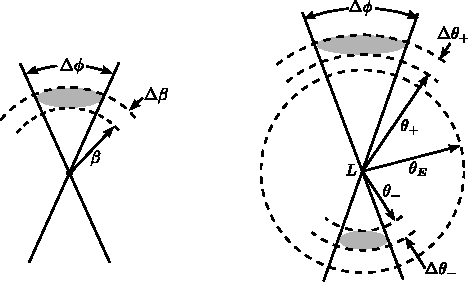
\includegraphics[width=0.6\textwidth]{../Images/Lensing_image_positions2.pdf}
				\caption[Schematic diagram of location of images]{Schematic diagram of location of images. The centre labelled L represents the observer-lens axis. The diagram on the left shows what would be observed if the lens was not present. The right hand diagram includes the effects of lensing\cite{Hartle}.\label{fig:Lensing_image_positions2}}
		\end{figure}

		In the case shown in Figure~\ref{fig:Lensing_image_positions2} where two visible images are observed, one image will form inside the Einstein radius ($\theta_{i+}$) and the other outside ($\theta_{i+}$). The positions of these two images are calculated by solving the Equation~\ref{eq:einstein_angle} giving
		\begin{align}
			\theta_{i\pm} &= \frac{1}{2}\left( \theta_S \pm {(\theta_S^2 + 4\theta_E^2)} ^{\frac{1}{2}} \right) \label{eq:image_position}
		\end{align}
		yielding the positions of the two unobstructed images as shown in Figure~\ref{fig:Lensing_image_positions2} one inside the Einstein radius, the other outside. Unlike optical lenses, gravitational lenses are achromatic, so the frequency of the light has no effect on the position of the images. As a result, images of the same object have exactly the same spectra and can easily be identified\cite{Hartle}.

		The azimuthal angle $\phi$ remains unchanged with and without the lens but as shown in figure lensing image positions, the polar angle and the width of the images are changed. The observed images are, therefore, stretched out into arcs and at any given radius will have the same curvature of a circle with origin at the centre of the lens\cite{Image_arc_curvature}. The change in the polar angle $\theta$ can be calculated by differentiating Equation~\ref{eq:image_position}, giving
		\begin{align}
			\Delta\theta_{i\pm} &= \frac{1}{2}\left( 1 \pm \frac{\theta_S}{(\theta_S^2 +4\theta_E^2)}^{\frac{1}{2}} \right) \Delta\theta_S
		\end{align}
		This shape distortion results from the fact that the sources are not point objects but in fact have light coming from a large area of the sky. The light from each end of the object will take different paths through the sky and will pass the lens at a different distance. The light will therefore be bent differently for different parts of the galaxy and the shape is distorted\cite{Arc_shapes_site}.

		The magnification of the source is given by the ratio of the image brightness to the source brightness. The surface brightness of any given source remains constant\cite{Hartle} but the effective solid angle $\Omega$ subtended by the detector is increased by the lens, hence the flux received by the detector, given by
		\begin{align}
			F &= (\text{surface brightness}) \times \Omega
		\end{align}
		is also increased. As the observed brightness of the source depends on the flux, the magnification is given by
		\begin{align}
			\mu &= \frac{F_{i\pm}}{F_S} = \frac{\Omega_{i\pm}}{\Omega_S}
			\intertext{Since in the small angle approximation, $\sin\theta \approx \theta$, the solid angles for the image and source are given by $\theta_{i\pm}\Delta\theta_{i\pm}\Delta\phi$ and $\theta_S \Delta_S \phi$ respectively. Given that $\Delta\phi$ is the same for both images, the magnification can be expressed as}
			\mu_{\pm} &= \left| \left( \frac{\theta_{i\pm}}{\theta_S} \dx{\theta_{i\pm}}{\theta_S} \right) \right| \\
			&=\frac{1}{4}\left( \frac{\theta_S}{{(\theta_S^2 +4\theta_E^2)}^{\frac{1}{2}}} + \frac{{(\theta_S^2 +4\theta_E^2)}^{\frac{1}{2}}}{\theta_S} \pm 2 \right)
			\intertext{For a lens modelled as a single isothermal sphere, this reduces to}
			\mu_\pm &= \frac{\theta_{i\pm}}{\theta_S} = \left( 1\mp \frac{\theta_E}{\theta_\pm} \right)^{-1}
		\end{align}
		The change in AB magnitude is then found using Equation~\ref{eq:magnitude_conversion}\cite{IOP_ABmagnification_site},
		\begin{align}
			\Delta m &= -2.5\log(\mu) \label{eq:magnitude_conversion}
		\end{align}
		The smaller the angle between the observer-lens axis and the source $\theta_S$, the greater the magnification of the source.
	% subsection concept (end)

% section gravitational_lensing (end)

    %!TEX root = mainfile.tex

\section{The Gunn-Peterson Effect} % (fold)
\label{sec:the_gunn_peterson_effect}
(Andrew)

	The current theoretical description of cosmic evolution at the end of the dark ages of the universe has gained widespread acceptance; as have the qualitative stages and processes of the epoch of reionisation. However, real empirical evidence from these eras remains sparse and clouded by large uncertainties. To accept the popular descriptions as fact without recourse to solid and quantitative evidence would be premature and in order to effectively investigate these high-redshifts, it is necessary to understand the spectral features of the objects we see in them.

	Along with measurements of the hydrogen \SI{21}{\centi\metre} line, the Gunn-Peterson effect and its impact on the spectra of distant galaxies are the two primary methods of observation currently being used to throw light on the epoch of reionisation and the early universe as a whole.

	\subsection{The Lyman Break} % (fold)
	\label{sub:the_lyman_break}
		The Lyman-$\alpha$ line is the spectral line corresponding to the $n=1$ to $n=2$ electron level transition in neutral hydrogen; it is the first transition in the Lyman series and the lowest energy level transition a hydrogen atom is capable of undergoing from its ground state. This transition is of particular relevance to cosmology and cosmic reionization, firstly, because during primordial nucleosynthesis, hydrogen atoms were created in the greatest abunance, with over 90\% of the produced atoms being hydrogen, approximately 8\% being Helium with smaller abundancies of other light elements \cite{BBNabundance}. Furthermore, during the epoch of reionization the average time between atomic excitations was large compared to the decay times of the excited states, meaning that the vast majority of HI atoms were in the ground state. This meant that the neutral IGM was highly resonant with photons of Lyman-$\alpha$ frequency, and was largely incapable of absorbtion of lower freqencies (ignoring the effects of fine and hyperfine line splitting).

		The proportion of radiation of some frequency which penetrates a medium is characterised by the medium's optical depth, $\tau$, for that wavelength, such that:
		\begin{align}
			I = I_0 e^{-\tau}. \label{eq:optical_depth}
		\end{align}
		The optical depth of neutral hydrogen to Lyman-$\alpha$ photons can be approximated by
		\begin{align}
			\tau_{GP} = 3.6 \times 10^5	\left ( 	\frac{\Omega_m h^2}{0.13}	\right ) ^{-1/2}
										\left ( 	\frac{\Omega_b h^2}{0.02}	\right )
										\left ( 	\frac{1+z}{7}			\right )^{3/2}
										\left ( 	\frac{n_{HI}}{n_H}			\right ) . \label{eq:gunn-peterson_tau}
		\end{align}
		The full derivation of this formula is given in appendix~\ref{app:derivation_of_the_gunn_peterson_optical_depth}.

		Using conventional values for $\Omega_b$ and $\Omega_m$ it can be shown that, for redshifts $>6$, the fraction of neutral hydrogen required to reduce the transmitted intensity to less than 1\% of the incident value is of the order of $10^{-5}$. Therefore, only a small amount of neutral hydrogen must occupy the intervening space between the distant galaxy and the observer to effectively eliminate the Lyman-$\alpha$ frequency from the object's spectrum.

		However, the frequency  of the absorbed radiation is not the Lyman-$\alpha$ line in the rest frame of the emitter, but in the rest frame of the absorber, such that as the light travels along its path to the observer successively shorter and shorter wavelengths are redshifted into resonance with the local neutral IGM and each wavelength is, in turn, scattered into extinction. This process continues untill the radiation reaches a region of spacetime where the hydrogen neutral fraction is significantly below the previously calculated value of $10^{-5}$.

		This effect, discovered by Gunn and Peterson in 1965, results in the extinction of a large portion of the flux from distant galaxies in the region blueward of the object's rest frame  Lyman-$\alpha$ line, known as the Lyman-$\alpha$ break, or the Gunn-Peterson trough.
		\begin{figure}[htbp]
			\centering
			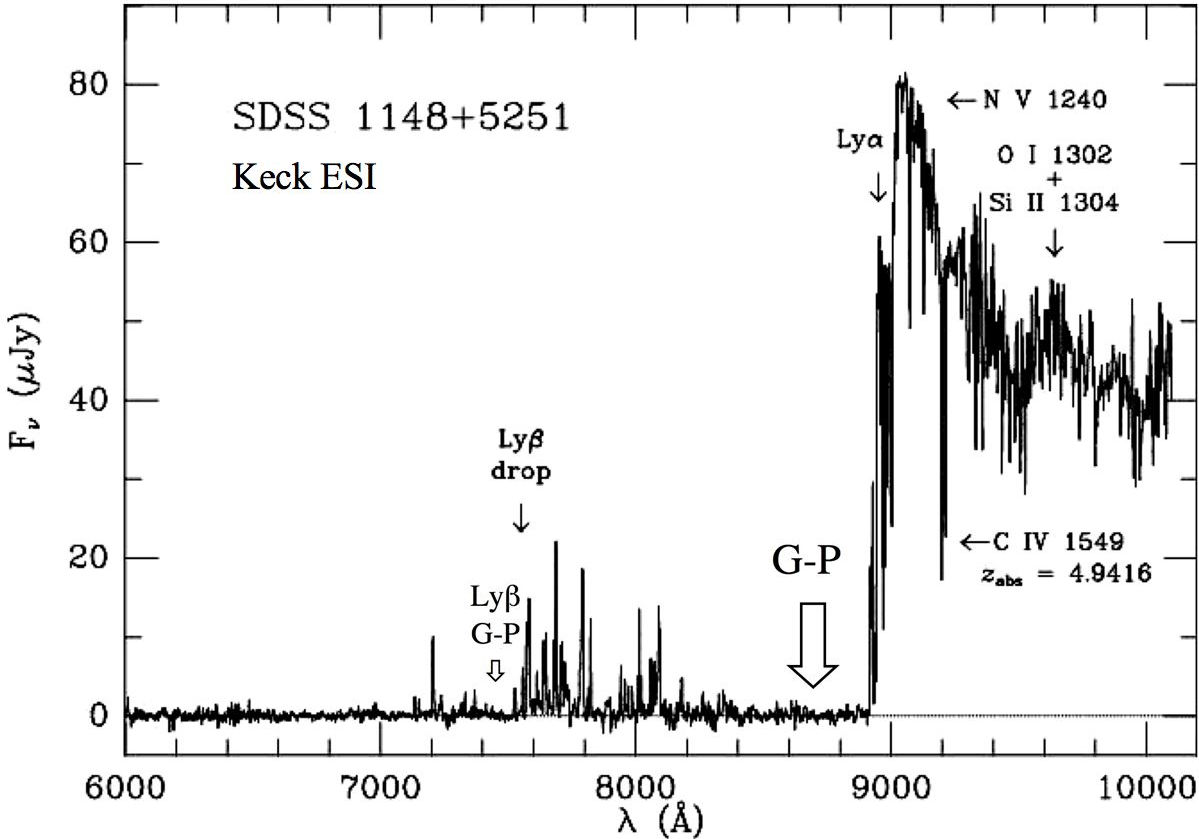
\includegraphics[width=0.7\textwidth]{../Images/dropout.jpg}
			\caption{Gunn-Peterson dropout in the spectrum of a galaxy at $z=6.4$.}\label{fig:dropout}
		\end{figure}

		The spectral flux from distant galaxies redward of the Lyman break is unaffected by Gunn-Peterson scattering and remains representative of the true brightness of the luminous object, while the region of the spectrum blueward of the break is highly obscured by the scattering effect of neutral hydrogen. While the portion of the true emitted spectrum in this region is lost, the extent of the loss contains infomation regarding the optical depth of the intervening space and, thereby, the density of neutral hydrogen at the redshift at which the Lyman break falls on that wavelength. Moreover, because the Lyman alpha line invariably falls at a specific point in the emitted spectrum, the redshift of any observed spectrum with an identifiable Lyman break can be measured easily. The break is such a strong spectral feature that it can be located even using broad band photometry, which is a significant advantage for objects at distances such that very little of their emitted light reaches us.
	% subsection the_lyman_break (end)

	\subsection{The Lyman-Alpha Forest} % (fold)
	\label{sub:the_lyman_alpha_forest}
		The neutral hydrogen distribution during cosmic reionization was not homogenous, with expanding bubbles of ionised IGM during the start of ionization and diminishing areas of neutral hydrogen after the central phase of rapid ionization. Regions of the IGM which are relatively underdense in neutral hydrogen have a correspondingly smaller optical depth to Lyman-$\alpha$ photons passing through them, resulting in sets of peaks on the blueward side of the Lyman break known as the Lyman-$\alpha$ forest.

		The Lyman forest peaks in figure~\ref{fig:dropout} are typical of galaxies at $z>5$ but the intesity fluctuations in the Lyman forest are largest in regions where the neutral hydrogen fraction is close to the critical value of $~10^{-5}$, such that even small fluctionations in ionised fraction lead to a large variation in transmitted intensity. An example of this is shown in figure~\ref{fig:forest}.
		\begin{figure}[htbp]
			\centering
			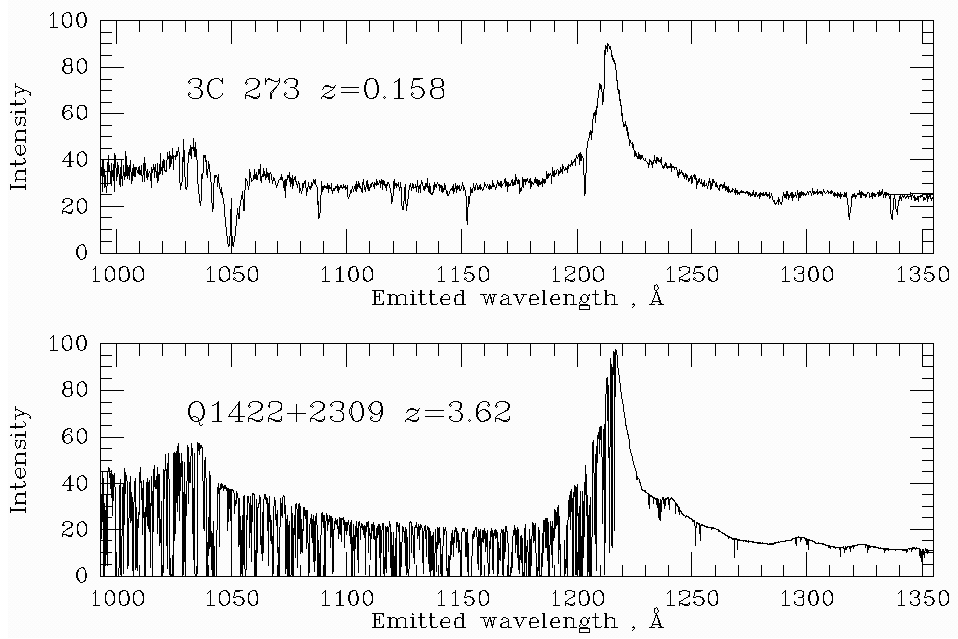
\includegraphics[width=0.7\textwidth]{../Images/forest.png}
			\caption{The spectra of two similar galaxies. Above: the spectrum of a galaxy at z=0.158 showing no significant extinction from Gunn-Peterson scattering. Below: the spectrum of a galaxy at z=3.62 showing a Lyman forest caused by fluctuations in hydrogen netrual fraction.}
			\label{fig:forest}
		\end{figure}

		It paradoxically seems, therefore, that the loss of flux caused by the Gunn-Peterson effect is extremely fortuitous to the observational cosmologist. Since the true emitted spectra of Lyman break galaxies are similar in nature to the spectra of closer galaxies with negligible Gunn-Peterson absorption, it is possible, in theory, to probe the density of neutral hydrogen at every point between the observed galaxy and the end of reionization.
	% subsection the_lyman_alpha_forest (end)

	\subsection{Properties of the Lyman Alpha Line} % (fold)
	\label{sub:properties_of_the_lyman_alpha_line}
		The full relativistic equation for the energy levels of neutral hydrogen was calculated by Dirac to be\cite{EisbergResnick}:
		\begin{align}
			E_{n,j} = - \frac{e^4}{ (4 \pi \epsilon_0)^2 2 \hbar^2 n^2} \left( \frac{m_p m_e}{m_p + m_e} \right) % E + R, p286
				\left [ 1 + \frac{\alpha^2}{n} \left( \frac{1}{j+1/2} - \frac{3}{4n} \right) \right]
		\end{align}
		Where n is the pricipal quantum number, j is the total spin eigenvalue and $\alpha$ is the fine structure constant:
		\begin{align}
			\alpha = \frac{e^2}{4 \pi \epsilon_0 \hbar c}  \approx \frac{1}{137}.
		\end{align}
		However, the final factor in square brackets is a small fractional correction of the order $10^{-5}$ or below and replacing the electron-proton reduced mass simply with the electron mass makes a fractional difference of the order of only $10^{-4}$. If both of these approximations are applied, the equation reduces to the more familiar relation for hydrogen energy levels which can be derived from the Bohr model of quantum mechanics
		\begin{align}
			E_n = - \frac{m_e e^4}{8 \epsilon_0^2 h^2 n^2}.
		\end{align}
		Using this result, the energy transfer of the n=2 to n=1 transition can then be calculated
		\begin{align}
			\Delta E_{2,1} &= E_2 - E_1 = 10.199\si{\electronvolt} ,
		\end{align}
		corresponding to a wavelength of:
		\begin{align}
			\lambda_{Ly\alpha} = \frac{hc}{\Delta E_{2,1}} = 1215.7 \si{\angstrom}.
		\end{align}
		This means the absorbed photons will invariably be ultraviolet in the absorber rest frame, but for objects observed during the epoch of reionization, cosmological redshift will push the observed Lyman break into the near infrared in the observer frame. The challenges of observing these wavelengths from such large distances and potential methods of overcoming them comprise a large portion of this report.
	% subsection properties_of_the_lyman_alpha_line (end)

%%%% resonance graph

%%%% fan picture of the troughs


% part general_theory (end)

\newpage
\part{Predictions} % (fold)
\label{prt:predictions}
    %!TEX root = mainfile.tex

\section{Predictions Group} % (fold)
\label{sec:predictions_group}
	In order for those attempting to observe high redshift galaxies to propose a detailed experimental plan, it is important to know how many galaxies one is expecting to observe within a certain volume of the sky. This is the fundamental purpose of the predictions sub-group; to be able to compute this quantity with the depth of the surveyed volume corresponding directly to redshift. In order to do this, a computer program is required to efficiently calculate this number as a function of redshift, field of view and apparent magnitude enabling those observing to make an informed prediction of the telescope one would need and the observing time required to make definitive observation of such elusive galaxies.

	This section of the project was structured chronologically as follows:
	\begin{itemize}
		\item Research how early galaxies are professionally predicted.
		\item Find a general Schechter function in terms of luminosity and/or magnitude.
		\item Mathematically process this function to ensure it is consistent with the units used by those carrying out the observations.
		\item Build a computer program to automate the process of calculating the number of galaxies from the Schechter function.
		\item Find plausible starting parameters to use in primary program.
		\item Collate parameter data from published papers.
		\item Determine parameter evolution with time.
		\item Plot these results to produce a visual description of how these parameters affect the outcome.
		\item Give expected number of galaxies to the observers.
		\item Refine technique with the inclusion of more advanced adaptations.
	\end{itemize}

	In addition to running a program to calculate the total number of galaxies, there is also a separate program to determine the redshifts at which re-ionization began and ended to be included when calculating the number of galaxies in the main code.

	The beginning of re-ionization has been determined by equating the star formation rate density with the critical star formation rate density required for matter to collapse into galaxies (see section..OWEN). The end of re-ionization occurs when the photons produced in star formation have completely ionized the IGM and hence required direct application of star formation rate densities also. This will be covered in more detail in section~\ref{sec:lower_redshift_limit_on_re-ionization}.

% section predictions_group (end)

    %!TEX root = mainfile.tex

\section{Assumptions Made} % (fold)
\label{sec:assumptions_made}
	The mathematical model that will be used in our program is limited by certain assumptions about the universe that we are working in. Some of these are generally held to be true and are accepted widely in the scientific community, others are due to the constraints of what we can mathematically program and the observational data available from previous studies. A major assumption that we are making throughout our work on re-ionisation concerns the type of universe that we exist in. A related pair of assumptions which have firm mathematical basis are the ``Cosmological Principle'' and the ``Isotropic Universe Theorem''. These state that our observations, as made from the Earth, are not subject to any influence from our location within it, in other words, we are not in a privileged position in the universe. This is assumed for almost all cosmological studies and shall not be considered.

	An important assumption that we are forced to make is that the Schechter function that we use describes our universe sufficiently to make predictions from. This is not as trivial as it sounds since the function is derived from data collected from much lower redshifts than some that we are considering. Further data will allow the accuracy of these functions to be improved. We have collected data and mathematical contributions from a number of high redshift studies to attempt to reduce the possibility of error and increase the accuracy of our function to as high a redshift as possible.

	For the early stages of our investigation, we will assume that both parameter evolution and cosmic variance do not influence the results. Clearly, these are big assumptions to make and so will be integrated into the calculations at later stages. This will be discussed further later.

	\subsubsection{AB Magnitude} % (fold)
	\label{ssub:ab_magnitude}
		In order to keep consistancy between the parts of this project, we have used the AB magnitude system throughout. This is a system for measuring the magnutide of an object in the sky. It is defined as
		\begin{align}
			M(AB) &= -2.5\log(f_\nu) -48.60
		\end{align}
		where $f_\nu$ is the monochormatic flux measured in \si{\erg\per\second\per\square\centi\metre\per\hertz}.
	% subsubsection ab_magnitude (end)

% section assumptions_made (end)

    %!TEX root = mainfile.tex

\section{Cosmological Distances} % (fold)
\label{sec:cosmological_distances}
	This section introduces some of the important distances used in various prediction calculations. First of all is the comoving distance between two observers at different redshifts. This is calculated via equation~(\ref{eq:comoving_distance})\cite{distance_measures_cosmology},
	\begin{align}
		D_{C}(z)=\frac{c}{H_{0}}\int^{z_{2}}_{z_{1}}\frac{\d{z'}}{E(z')} \label{eq:comoving_distance}
	\end{align}
	where $E(z)$ is the dimensionless Hubble parameter which is,
	\begin{align}
		E(z)=\sqrt{\Omega_{M}{(1+z)}^{3}+\Omega_{R}{(1+z)}^{4}+\Omega_{\Lambda}}
	\end{align}
	Where $\Omega_{M}$, $\Omega_{R}$ and $\Omega_{\Lambda}$ are the different density parameters for mass, radiation and dark energy respectively.

	To calculate the comoving distance to an object at a particular redshift the integral above must be done for $z_{1}=0$ up to an arbitrary $z$. Comoving distance is the distance between two comoving observers i.e.\ both moving with respect to the Hubble flow (factoring out the expansion of the universe). In the project this has been used to determine a volume of space for a given redshift range. This was done by finding the volume difference between two shells of comoving radius at two different redshifts.

	The luminosity distance is the distance that a photon travels from a source to an observer. As a photon will undergo a Doppler shift and be redshifted into longer wavelengths (red part of the spectrum). Therefore the luminosity distance is essentially a redshifted transverse comoving distance\cite{distance_measures_cosmology}, which for a flat universe is the comoving distance therefore,
	\begin{align}
		D_{L}(z)=(1+z)D_{C}(z)
	\end{align}
	In this project the luminosity distance has been used to convert between magnitudes, luminosity and flux.

	Also, the angular diameter distance is simply the proper distance along a radius $r_{e}$ where this is the radius at the time of emission. Therefore angular diameter distance is,
	\begin{align}
		D_{A} &= r_{e}a_{e} = \frac{a_{0}r_{e}}{1+z_{e}}
		\intertext{where $a_{0}r_{e}$ in a flat universe is the same as,}
		D_{A}(z) &= \frac{D_{C}}{1+z}
	\end{align}
	This is used to convert angular seperations in telescope images to actual angular seperations and then can determine the size of objects\cite{distance_measures_cosmology}.
% section cosmological_distances (end)

    %!TEX root = mainfile.tex

\section{Cosmological Distances} % (fold)
\label{sec:cosmological_distances}
	This section introduces some of the important distances used in various prediction calculations. First of all is the comoving distance between two observers at different redshifts. This is calculated via equation~\ref{fig:comoving_distance}\cite{distance_measures_cosmology},
	\begin{align}
		D_{C}(z)=\frac{c}{H_{0}}\int^{z_{2}}_{z_{1}}\frac{\d{z'}}{E(z')} \label{fig:comoving_distance}
	\end{align}
	where $E(z)$ is the dimensionless Hubble parameter which is,
	\begin{align}
		E(z)=\sqrt{\Omega_{M}{(1+z)}^{3}+\Omega_{R}{(1+z)}^{4}+\Omega_{\Lambda}}
	\end{align}
	Where $\Omega_{M}$, $\Omega_{R}$ and $\Omega_{\Lambda}$ are the different density parameters for mass, radiation and dark energy respectively.

	To calculate the comoving distance to an object at a particular redshift the integral above must be done for $z_{1}=0$ up to an arbitrary $z$. Comoving distance is the distance between two comoving observers i.e.\ both moving with respect to the Hubble flow (factoring out the expansion of the universe). In the project this has been used to determine a volume of space for a given redshift range. This was done by finding the volume difference between two shells of comoving radius at two different redshifts.

	The luminosity distance is the distance that a photon travels from a source to an observer. As a photon will undergo a Doppler shift and be redshifted into longer wavelengths (red part of the spectrum). Therefore the luminosity distance is essentially a redshifted transverse comoving distance\cite{distance_measures_cosmology}, which for a flat universe is the comoving distance therefore,
	\begin{align}
		D_{L}(z)=(1+z)D_{C}(z)
	\end{align}
	In this project the luminosity distance has been used to convert between magnitudes, luminosity and flux.

	Also, the angular diameter distance is simply the proper distance along a radius $r_{e}$ where this is the radius at the time of emission. Therefore angular diameter distance is,
	\begin{align}
		D_{A} &= r_{e}a_{e} = \frac{a_{0}r_{e}}{1+z_{e}}
		\intertext{where $a_{0}r_{e}$ in a flat universe is the same as,}
		D_{A}(z) &= \frac{D_{C}}{1+z}
	\end{align}
	This is used to convert angular seperations in telescope images to actual angular seperations and then can determine the size of objects\cite{distance_measures_cosmology}.
% section cosmological_distances (end)

\section{Schechter Function} % (fold)
\label{sec:schechter_function}
	One important part of our project is to determine the luminosity function at high redshift, which is a plot of the number density of galaxies binned against their respective luminosities. A schechter function is used to fit this luminosity function. A schechter function is a form that has a power law which has a certain cut-off at which it becomes an exponential curve. The schechter function in terms of luminosity i.e.\ the luminosity function is shown in equation~\ref{eq:shechter_luminosity}\cite{cosmo_number_densities}.
	\begin{align}
		\phi(L)=\frac{\phi^{*}}{L^{*}}\frac{L}{L^{*}}^{\alpha}e^{-L/L^{*}} \label{eq:shechter_luminosity}
	\end{align}
	$\phi^{*}$ is the normalization factor in units of \si{\per\mega\parsec\cubed}, $\alpha$ is the gradient of the faint end slope of the luminosity function and $L^{*}$ is the characteristic luminosity at which the function changes from a power law to an exponential cut off. Therefore there are a majority of lower luminosity galaxies and not many bright ones.

	There are two basic methods to determine the best fit parameters of the schechter function\cite{luminosity_functions_online}. The first one is to take cluster samples and bin them by apparent magnitude then fit a schechter function trying to minimize the error. The other way is to use the ``maximum likelihood method''. This method takes a flux limited sample and finds the probability that a galaxy actually has a particular luminiostity at respective distances and then define a likelihood function which is the joint probability of finding all luminosities at their respective distances. These are then the most likely parameters consistent with the data and a schechter form. However in this project schechter parameters were simply cited from various articles as we are not doing any observations ourselves to get our predictions.

	The luminosity function can then be integrated to find the number density in \si{\per\mega\parsec\cubed},
	\begin{align}
		\rho_{N}=\int^{\infty}_{L}\phi(L)\d{L}
	\end{align}
	Where $L$ is the lower limit luminosity that can be seen in the universe, this is needed as the luminosity function tends to infinity at the faint end.

	It is easier to plot the luminosity function on the log scale and therefore most of the papers we cite state the absolute magnitude schechter function instead which is obtained by substituting,
	\begin{align}
		\frac{L}{L*}=10^{0.4(M^{*}-M)}
	\end{align}
	which is then multiplied by the derivative and rearranged to get the equation,
	\begin{align}
		\phi(M)=\phi^{*}(\ln(10)){\left[10^{0.4(M^{*}-M)}\right]}^{\alpha+1}\e{\left[-10^{0.4(M^{*}-M)}\right]}
	\end{align}
	Where $M^{*}$ is the characteristic absolute magnitude where the cut off happens.

	However a range of apparent magnitudes is normally observed, rather than absolute magnitudes and so the absolute magnitude equation above is changed to it's apparent magnitude form, using the simple relationship below,
	\begin{align}
		m=M+5((\log_{10}D_{L})-1)
	\end{align}
	Where $D_{L}$ is the luminosity distance. Note that the derivative of this substitution is 1 and so does not need to be accounted for.

	Or the luminosity density of galaxies in \si{\erg\per\second\per\mega\parsec\cubed\per\hertz} can also be calculated using,
	\begin{align}
		\rho_{L}=\int^{\infty}_{L}L\phi(L)dL
	\end{align}
	This will become useful for calculating star formation rates in later sections.
% section schechter_function (end)

\section{Lower Redshift limit on Re-ionization} % (fold)
\label{sec:lower_redshift_limit_on_re-ionization}
	In the project the way that the lower redshift limit has been calculated is to first calculate the rate of photons capable of ionizing a hydrogen atom via equation~\ref{eq:rate_of_ionising_photons}\cite{2010Natur.468...49R}.
	\begin{align}
		\frac{\d{n_{ion}}}{\d{t}}=f_{esc}\zeta\rho_\text{SFR}\label{eq:rate_of_ionising_photons}
	\end{align}
	Where $f_{esc}$ is the fraction of ionizing photons that escape a galaxy, $\zeta$ is the number of hydrogen-ionizing photons produced per second per unit star formation rate and $\rho_\text{SFR}$ is the star formation rate per unit volume.

	Therefore by integrating this equation up to the age of the universe at a specific redshift a total number of photons capable of ionizing the universe can be outputted. The number of ionizing photons are then equated to the total number of hydrogen atoms in the IGM of the universe to get a lower redshift limit of re-ionization.

	First of all the program gets the critical density of the universe by,
	\begin{align}
		\rho_{crit}(z)=\frac{3H{(z)}^{2}}{8\pi G}
	\end{align}
	Then by multiplying this by the baryonic density parameter, $\Omega_{b}=0.045\pm0.004$, the baryonic density is achieved. By then multiplying by the fraction of hydrogen, calculated from big bang nucleosynthesis, the total density of hydrogen in the universe can be obtained.

	From the 7 year WMAP survey\cite{2011ApJS..192...18K}, we can get the primordial Helium fraction to be $Y=0.33\pm0.09$. Where we assume that Hydrogen fraction ($X$) is simply $1-Y$ (therefore 0 metallicity). Although a simplifying assumption it is not too bad as the errors on fraction of helium are higher than the actual fraction of heavier elements.

	Then finally dividing the mass density of hydrogen by the atomic mass unit the code obtains a number density of hydrogen. In the code a redshift time relation $\frac{1}{(1+z)}\propto t^{2/3}$, assuming a matter dominated universe, is used and therefore,
	\begin{align}
		t &= \frac{t_{0}}{{(1+z)}^{3/2}} \\
		\Rightarrow \dx{t}{z} &= \frac{3}{2}\frac{t_{0}}{{(1+z)}^{5/2}}
	\end{align}

	In the first version of the code, values of star formation rate densities from  various articles with redshifts varying from redshifts 4 to up to about 8 from\cite{2010MNRAS.401.2561W}, which determine star formation rates from observations of Gamma-ray bursts (GRBs) from deaths of massive short lived stars which can be directly related to star formation rate. Also compiling these values with those from\cite{2012ApJ...759L..38A}, which use a semi-analytical model to determine star formation rates from redshifts 9 to 16. These two papers with very different methods have surprising correlation in values.

	These values were then plotted against redshift. The function of redshift that was used for $\rho_\text{SFR}$ was,
	\begin{align}
		\rho_\text{SFR}(z)=0.399(\pm 0.181)\e{-0.253(\pm 0.118)z}-0.011(\pm 0.025)
	\end{align}
	However this equation will only work up to a redshift of around 5 as the star formation rate for galaxies will drop with redshifts lower than this due to the gas being used up and star formation will drop off. This should not effect our results too much however as the project tends to study redshifts higher than this anyway. Also there will be large errors on higher redshift values due to problems with extrapolating the data, and unrealistic numbers of star formation where in reality there would be none.
	%Reference to beth's section
	We also used rough estimates of $f_\text{esc}=0.2$ and $\zeta=10^{53.5}$ as stated in section~\ref{???}.

	The code also used a function of the global stellar mass density to figure out the amount of hydrogen that was calculated was in stars at a given redshift. This therefore gives us a certain fraction that is not part of the IGM and does not need to be ionized. These values were taken from the direct observations of three papers \cite{2006A&A...459..745F}, \cite{2003A&A...401...73W} and \cite{2003ApJS..149..289B}. The function of redshift that was calculated was,
	\begin{align}
		\rho_\text{stellar}(M_{\odot}\si{\per\mega\parsec\cubed})=\e{-0.81z+19.7}
	\end{align}
	but this does not have much effect on the number of hydrogen as the stellar fraction is very small, so this is not a significant contributing factor.

	The code then loops for different values of redshift from redshift 25 at redshift intervals of 0.1, calculating the number of ionizing photons at those different epochs and equating this to the hydrogen number. This then outputs ionized fraction against redshift, shown in figure \ref{fig:IonizedFraction1}.
	\begin{figure}[!htb]
		\centering
			\begingroup\endlinechar=-1
		  		\resizebox{0.7\textwidth}{!}{%
					% GNUPLOT: LaTeX picture with Postscript
\begingroup
  \makeatletter
  \providecommand\color[2][]{%
    \GenericError{(gnuplot) \space\space\space\@spaces}{%
      Package color not loaded in conjunction with
      terminal option `colourtext'%
    }{See the gnuplot documentation for explanation.%
    }{Either use 'blacktext' in gnuplot or load the package
      color.sty in LaTeX.}%
    \renewcommand\color[2][]{}%
  }%
  \providecommand\includegraphics[2][]{%
    \GenericError{(gnuplot) \space\space\space\@spaces}{%
      Package graphicx or graphics not loaded%
    }{See the gnuplot documentation for explanation.%
    }{The gnuplot epslatex terminal needs graphicx.sty or graphics.sty.}%
    \renewcommand\includegraphics[2][]{}%
  }%
  \providecommand\rotatebox[2]{#2}%
  \@ifundefined{ifGPcolor}{%
    \newif\ifGPcolor
    \GPcolortrue
  }{}%
  \@ifundefined{ifGPblacktext}{%
    \newif\ifGPblacktext
    \GPblacktexttrue
  }{}%
  % define a \g@addto@macro without @ in the name:
  \let\gplgaddtomacro\g@addto@macro
  % define empty templates for all commands taking text:
  \gdef\gplbacktext{}%
  \gdef\gplfronttext{}%
  \makeatother
  \ifGPblacktext
    % no textcolor at all
    \def\colorrgb#1{}%
    \def\colorgray#1{}%
  \else
    % gray or color?
    \ifGPcolor
      \def\colorrgb#1{\color[rgb]{#1}}%
      \def\colorgray#1{\color[gray]{#1}}%
      \expandafter\def\csname LTw\endcsname{\color{white}}%
      \expandafter\def\csname LTb\endcsname{\color{black}}%
      \expandafter\def\csname LTa\endcsname{\color{black}}%
      \expandafter\def\csname LT0\endcsname{\color[rgb]{1,0,0}}%
      \expandafter\def\csname LT1\endcsname{\color[rgb]{0,1,0}}%
      \expandafter\def\csname LT2\endcsname{\color[rgb]{0,0,1}}%
      \expandafter\def\csname LT3\endcsname{\color[rgb]{1,0,1}}%
      \expandafter\def\csname LT4\endcsname{\color[rgb]{0,1,1}}%
      \expandafter\def\csname LT5\endcsname{\color[rgb]{1,1,0}}%
      \expandafter\def\csname LT6\endcsname{\color[rgb]{0,0,0}}%
      \expandafter\def\csname LT7\endcsname{\color[rgb]{1,0.3,0}}%
      \expandafter\def\csname LT8\endcsname{\color[rgb]{0.5,0.5,0.5}}%
    \else
      % gray
      \def\colorrgb#1{\color{black}}%
      \def\colorgray#1{\color[gray]{#1}}%
      \expandafter\def\csname LTw\endcsname{\color{white}}%
      \expandafter\def\csname LTb\endcsname{\color{black}}%
      \expandafter\def\csname LTa\endcsname{\color{black}}%
      \expandafter\def\csname LT0\endcsname{\color{black}}%
      \expandafter\def\csname LT1\endcsname{\color{black}}%
      \expandafter\def\csname LT2\endcsname{\color{black}}%
      \expandafter\def\csname LT3\endcsname{\color{black}}%
      \expandafter\def\csname LT4\endcsname{\color{black}}%
      \expandafter\def\csname LT5\endcsname{\color{black}}%
      \expandafter\def\csname LT6\endcsname{\color{black}}%
      \expandafter\def\csname LT7\endcsname{\color{black}}%
      \expandafter\def\csname LT8\endcsname{\color{black}}%
    \fi
  \fi
  \setlength{\unitlength}{0.0500bp}%
  \begin{picture}(7200.00,4320.00)%
    \gplgaddtomacro\gplbacktext{%
      \put(747,595){\makebox(0,0)[r]{\strut{} 0}}%
      \put(747,1182){\makebox(0,0)[r]{\strut{} 0.2}}%
      \put(747,1768){\makebox(0,0)[r]{\strut{} 0.4}}%
      \put(747,2355){\makebox(0,0)[r]{\strut{} 0.6}}%
      \put(747,2942){\makebox(0,0)[r]{\strut{} 0.8}}%
      \put(747,3528){\makebox(0,0)[r]{\strut{} 1}}%
      \put(747,4115){\makebox(0,0)[r]{\strut{} 1.2}}%
      \put(849,409){\makebox(0,0){\strut{} 0}}%
      \put(2058,409){\makebox(0,0){\strut{} 5}}%
      \put(3267,409){\makebox(0,0){\strut{} 10}}%
      \put(4475,409){\makebox(0,0){\strut{} 15}}%
      \put(5684,409){\makebox(0,0){\strut{} 20}}%
      \put(6893,409){\makebox(0,0){\strut{} 25}}%
      \csname LTb\endcsname%
      \put(144,2355){\rotatebox{-270}{\makebox(0,0){\strut{}Ionised Fraction ($X$)}}}%
      \csname LTb\endcsname%
      \put(3871,130){\makebox(0,0){\strut{}Redshift (z)}}%
      \put(3871,4022){\makebox(0,0){\strut{}}}%
    }%
    \gplgaddtomacro\gplfronttext{%
      \csname LTb\endcsname%
      \put(6105,3948){\makebox(0,0)[r]{\strut{}Best Fit}}%
      \csname LTb\endcsname%
      \put(6105,3762){\makebox(0,0)[r]{\strut{}Lower Limit}}%
      \csname LTb\endcsname%
      \put(6105,3576){\makebox(0,0)[r]{\strut{}Upper Limit}}%
    }%
    \gplbacktext
    \put(0,0){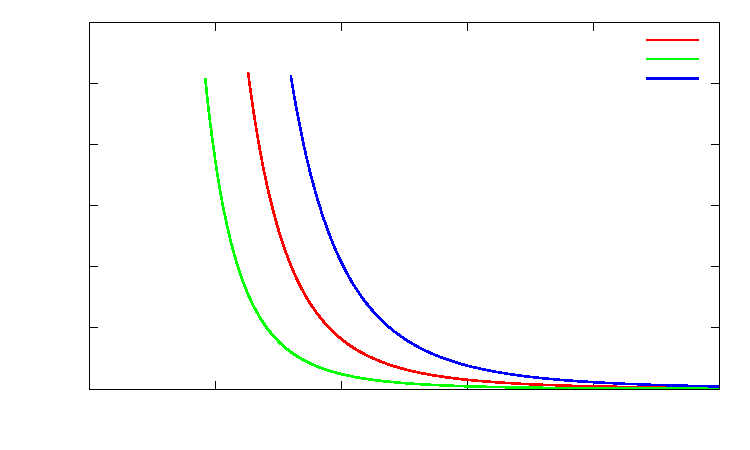
\includegraphics{GRAPH_StellarDens_exponential}}%
    \gplfronttext
  \end{picture}%
\endgroup

		  		}\endgroup
		\caption{Plot of modeled ionized fraction of the IGM as a function of redshift.\label{fig:IonizedFraction1}}
	\end{figure}

	From this we get that the universe is completely ionized at a redshift $6.3\pm1.7$, ignoring the rather large errors, this number is not a bad estimate of the epoch. We know this from articles which show from observations of Lyman-$\alpha$ emitters that there must be a large ionized fraction at 6.5, due to attenuation from neutral hydrogen\cite{Ota:arXiv0707.1561}. Various theoretical models of star formation rate predict a ionized universe at around 6 and it is stated that the Sunyaev-Zeldovich effect has put a limit that Reionization ends earlier than 5.8 \cite{2012MNRAS.423..862K}.

	However as recombination has not been included which will slow down the rate at which the universe is ionized or the fact that both the escape fraction and $\zeta$ are likely to change with redshift, this number is not actually realistic.

	\subsection{Evolving Escape Fraction} % (fold)
	\label{sub:evolving_escape_fraction}
		As already stated the previous results make a basic assumption of of the escape fraction to be about $20\%$ during the epoch of reionization. This is obviously not a very good assumption as it will evolve with redshift. However there lies a problem in this which is related to the previous section, section~\ref{???}(Beth's bit on fesc) which explained the difficulty in measuring this parameter as well as the problems in extrapolating out to higher redshifts much like in our star formation rates. This uncertainty in the measure is what leads to the differences stated in\cite{2012ApJ...759L..38A}, which states a higher fraction at higher redshift due to lack of dust, and\cite{2000ApJ...545...86W} which states the opposite, due to increasing disk densities and increasing density in the universe as a whole. However from\cite{2012arXiv1209.2123F} and\cite{2013MNRAS.428L...1M} by using recent semi-analytical model they found that the escape fraction does indeed increase with redshift and so this is the model that is used in this project.

		Once again using the fit program to fit a exponential to the escape fraction measurements and predictions from\cite{2012ApJ...759L..38A},\cite{2006ApJ...651L..89R} and\cite{2006MNRAS.371L...1I}. The functional form that is achieved is,
		\begin{align}
			f_\text{esc}(z)=\e{0.013\pm0.011-0.952\pm0.06}
		\end{align}
		The code is then run again with this escape fraction instead of the constant $20\%$, the results achieved are shown in \ref{fig:IonizedFraction2}
		\begin{figure}
			\centering
				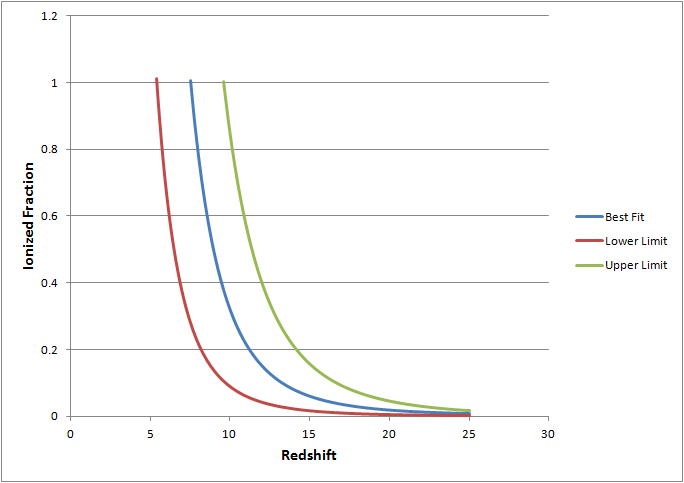
\includegraphics[width=0.8\textwidth]{F:/Extragalactic cosmology/IonizedFraction2.png}
				\caption{Plot of modeled ionized fraction of the IGM as a function of redshift with predicting evolving escape fraction.\label{fig:IonizedFraction2}}
		\end{figure}

		The graph in figure~\ref{fig:IonizedFraction2} shows that the addition of the evolving escape fraction has resulted in the universe being ionized quicker which is what is expected, since recombinations have not been included in this model. This model outputs a redshift of $7.5\pm2.1$, which shows the increase in redshift and also in error due to the error on $f_\text{esc}$ itself. It is very hard to determine whether this is an improvement or a hindrance to the previous model just due to the errors on measuring/predicting f_{esc}.

		%Not completed having trouble with it not sure if it should be included without conclusive results?
	% subsection evolving_escape_fraction (end)

	\subsection{Recombinations} % (fold)
	\label{sub:recombinations}
		To include Recombinations into our project, the rate at which hydrogen will recombine. The mean recombination time was found in \cite{2012MNRAS.423..862K} to be,
		\begin{align}
			\bar{t}_\text{rec} &= \frac{1}{C_{HII}\alpha_{B}(T_{0})\bar{n}_{H}(1+Y/4X)(1+z)^{3}}\\
			&\approx 0.93Gyr\left(\frac{3}{C_{HII}}\right)\left(\frac{T_{0}}{2\times 10^{4}K}\right)^{0.7}\left(\frac{7}{1+z}\right)^{3}
		\end{align}
		Where $C_{HII}$ is the clumping factor of ionized hydrogen and $T_{0}$ is the mean IGM temperature. Both of these values are plotted and fitted against redshift exactly in the same way as previous parameters. Where values of the clumping factor against redshift are cited from a theoretical model in\cite{2011MNRAS.412L..16R} and the IGM mean temperature is cited from\cite{2006MNRAS.373.1265O} based on simulations.

		The code then takes this equation for the mean recombination time of hydrogen and integrates the inverse of this from 0 to the specific $t(z)$. This will give us a mean total of hydrogen that will have recombined in that time period. However when this method is implemented into the code and ran, it outputs values of recombination that are insignificant because they are so low. This seems unphysical as we would expect the recombinations in the universe to be much higher than this and make a significant contribution to the rate at which the universe ionizes.
	% subsection recombinations (end)

% section lower_redshift_limit_on_re-ionization (end)

        %!TEX root = mainfile.tex

\section{Parameter Values} % (fold)
\label{sec:parameter_values}
    There are also a number of parameters in the Schechter function that must be specified. In order to find suitable values to use, we collected data from a number of different sources covering several studies. All of the studies that have been performed in the past concern galaxies at lower redshifts than we are expecting to examine. To get an estimate for the value of each of the parameters at higher redshift, the values found were plotted and the fit extrapolated to cover the era necessary. Since some of the fits demonstrate that these parameters are not constant with time, their evolution shall be incorporated into the calculations.

    The values in the Schechter function that we have determined fits for are $\alpha$, $M^{*}$ and $\phi^{*}$. The data collected for each of these fits is shown in appendix~\ref{app:parameter_fit_data}.

    \subsection{Parameter Evolution} % (fold)
    \label{sub:parameter_evolution}
        The early stages of the models we used assumed that the parameters of the Schechter function were static with respect to time. This means that, when iterating over the redshift, the only property that changed was the co-moving volume. This is non-physical since it does not allow for changes in the characteristic mass and characteristic luminosity for different conditions in the universe. In order to improve the model, we collected data from a number of previous studies for three values, the characteristic mass, $M^*$, the Schechter normalisation, $\phi^*$ and the faint end slope parameter, $\alpha$.

        \subsubsection{Linear Parameter Evolution with Redshift} % (fold)
        \label{ssub:linear_parameter_evolution_with_redshift}

            In order to provide useful errors on the fits of the parameters, a technique called the pivot fit method is used to decouple the errors on $y$-intercept and gradient. This involved fitting the data after it has been normalised around the mean value. This normalisation simply involves taking the mean $x$- and $y$-value from each data point so that the graph is centred about the origin. This means that the $y$-intercept is fixed to zero and thus the fitting error applies only to the gradient. Subsequent linear fits shall be treated in this manner, so that errors quoted correspond to the gradient. For clarity of presentation, the data shall be plotted in its original form.

            The graph in figure~\ref{fig:alpha_evolution} shows the data collected, with the corresponding uncertainties, for the linear parameter, $\alpha$. From this data, a linear fit is taken. The relevant evolution, then, is governed by the equation $\alpha = -0.015z - 1.664$.
            \begin{figure}[!htb]
                \centering
                    \begingroup\endlinechar=-1
                        \resizebox{0.6\textwidth}{!}{%
                            % GNUPLOT: LaTeX picture with Postscript
\begingroup
  \makeatletter
  \providecommand\color[2][]{%
    \GenericError{(gnuplot) \space\space\space\@spaces}{%
      Package color not loaded in conjunction with
      terminal option `colourtext'%
    }{See the gnuplot documentation for explanation.%
    }{Either use 'blacktext' in gnuplot or load the package
      color.sty in LaTeX.}%
    \renewcommand\color[2][]{}%
  }%
  \providecommand\includegraphics[2][]{%
    \GenericError{(gnuplot) \space\space\space\@spaces}{%
      Package graphicx or graphics not loaded%
    }{See the gnuplot documentation for explanation.%
    }{The gnuplot epslatex terminal needs graphicx.sty or graphics.sty.}%
    \renewcommand\includegraphics[2][]{}%
  }%
  \providecommand\rotatebox[2]{#2}%
  \@ifundefined{ifGPcolor}{%
    \newif\ifGPcolor
    \GPcolortrue
  }{}%
  \@ifundefined{ifGPblacktext}{%
    \newif\ifGPblacktext
    \GPblacktexttrue
  }{}%
  % define a \g@addto@macro without @ in the name:
  \let\gplgaddtomacro\g@addto@macro
  % define empty templates for all commands taking text:
  \gdef\gplbacktext{}%
  \gdef\gplfronttext{}%
  \makeatother
  \ifGPblacktext
    % no textcolor at all
    \def\colorrgb#1{}%
    \def\colorgray#1{}%
  \else
    % gray or color?
    \ifGPcolor
      \def\colorrgb#1{\color[rgb]{#1}}%
      \def\colorgray#1{\color[gray]{#1}}%
      \expandafter\def\csname LTw\endcsname{\color{white}}%
      \expandafter\def\csname LTb\endcsname{\color{black}}%
      \expandafter\def\csname LTa\endcsname{\color{black}}%
      \expandafter\def\csname LT0\endcsname{\color[rgb]{1,0,0}}%
      \expandafter\def\csname LT1\endcsname{\color[rgb]{0,1,0}}%
      \expandafter\def\csname LT2\endcsname{\color[rgb]{0,0,1}}%
      \expandafter\def\csname LT3\endcsname{\color[rgb]{1,0,1}}%
      \expandafter\def\csname LT4\endcsname{\color[rgb]{0,1,1}}%
      \expandafter\def\csname LT5\endcsname{\color[rgb]{1,1,0}}%
      \expandafter\def\csname LT6\endcsname{\color[rgb]{0,0,0}}%
      \expandafter\def\csname LT7\endcsname{\color[rgb]{1,0.3,0}}%
      \expandafter\def\csname LT8\endcsname{\color[rgb]{0.5,0.5,0.5}}%
    \else
      % gray
      \def\colorrgb#1{\color{black}}%
      \def\colorgray#1{\color[gray]{#1}}%
      \expandafter\def\csname LTw\endcsname{\color{white}}%
      \expandafter\def\csname LTb\endcsname{\color{black}}%
      \expandafter\def\csname LTa\endcsname{\color{black}}%
      \expandafter\def\csname LT0\endcsname{\color{black}}%
      \expandafter\def\csname LT1\endcsname{\color{black}}%
      \expandafter\def\csname LT2\endcsname{\color{black}}%
      \expandafter\def\csname LT3\endcsname{\color{black}}%
      \expandafter\def\csname LT4\endcsname{\color{black}}%
      \expandafter\def\csname LT5\endcsname{\color{black}}%
      \expandafter\def\csname LT6\endcsname{\color{black}}%
      \expandafter\def\csname LT7\endcsname{\color{black}}%
      \expandafter\def\csname LT8\endcsname{\color{black}}%
    \fi
  \fi
  \setlength{\unitlength}{0.0500bp}%
  \begin{picture}(7200.00,4320.00)%
    \gplgaddtomacro\gplbacktext{%
      \put(747,915){\makebox(0,0)[r]{\strut{}-2.2}}%
      \put(747,1555){\makebox(0,0)[r]{\strut{}-2}}%
      \put(747,2195){\makebox(0,0)[r]{\strut{}-1.8}}%
      \put(747,2835){\makebox(0,0)[r]{\strut{}-1.6}}%
      \put(747,3475){\makebox(0,0)[r]{\strut{}-1.4}}%
      \put(747,4115){\makebox(0,0)[r]{\strut{}-1.2}}%
      \put(849,409){\makebox(0,0){\strut{} 0}}%
      \put(2058,409){\makebox(0,0){\strut{} 2}}%
      \put(3267,409){\makebox(0,0){\strut{} 4}}%
      \put(4475,409){\makebox(0,0){\strut{} 6}}%
      \put(5684,409){\makebox(0,0){\strut{} 8}}%
      \put(6893,409){\makebox(0,0){\strut{} 10}}%
      \csname LTb\endcsname%
      \put(144,2355){\rotatebox{-270}{\makebox(0,0){\strut{}Faint End Slope ($\alpha$)}}}%
      \csname LTb\endcsname%
      \put(3871,130){\makebox(0,0){\strut{}Redshift ($z$)}}%
      \put(3871,4022){\makebox(0,0){\strut{}}}%
    }%
    \gplgaddtomacro\gplfronttext{%
      \csname LTb\endcsname%
      \put(3297,762){\makebox(0,0)[r]{\strut{}$f(x) = -0.015x + -1.664$}}%
    }%
    \gplbacktext
    \put(0,0){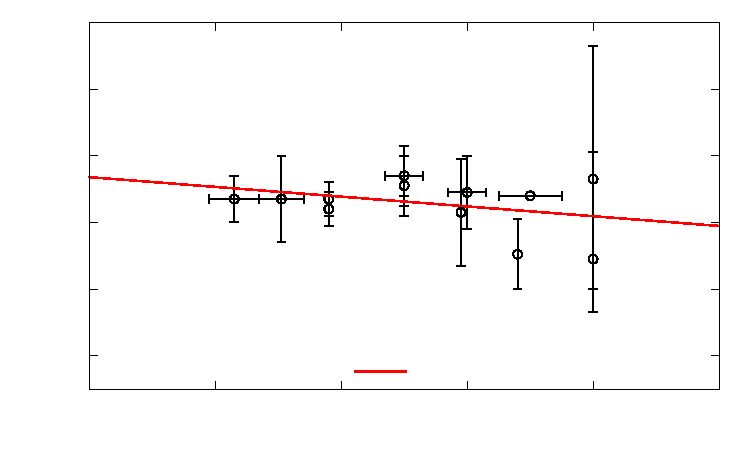
\includegraphics{GRAPH_Parameter_Fit_alpha_linear}}%
    \gplfronttext
  \end{picture}%
\endgroup

                        }\endgroup
                \caption{The evolution of $\alpha$ as a function of redshift according to past observational studies.\label{fig:alpha_evolution}}
            \end{figure}

            Figure~\ref{fig:phi_evolution} shows the data for the evolution of the normalisation parameter $\phi^{*}$. This value is known to be never less than zero. For this reason, coupled with an attempt to reduce the errors as far as possible, an exponential decrease with redshift was chosen. Although the errors for this fit are large, because of the errors on the data points, the region of concern, high redshift greater than 6, this evolution can be approximated to zero. In other words, during the times that we are considering, it can be approximated that there was no change in the value of the normalisation parameter, $\phi^*$.
            \begin{figure}[!htb]
                \centering
                    \begingroup\endlinechar=-1
                        \resizebox{0.6\textwidth}{!}{%
                            % GNUPLOT: LaTeX picture with Postscript
\begingroup
  \makeatletter
  \providecommand\color[2][]{%
    \GenericError{(gnuplot) \space\space\space\@spaces}{%
      Package color not loaded in conjunction with
      terminal option `colourtext'%
    }{See the gnuplot documentation for explanation.%
    }{Either use 'blacktext' in gnuplot or load the package
      color.sty in LaTeX.}%
    \renewcommand\color[2][]{}%
  }%
  \providecommand\includegraphics[2][]{%
    \GenericError{(gnuplot) \space\space\space\@spaces}{%
      Package graphicx or graphics not loaded%
    }{See the gnuplot documentation for explanation.%
    }{The gnuplot epslatex terminal needs graphicx.sty or graphics.sty.}%
    \renewcommand\includegraphics[2][]{}%
  }%
  \providecommand\rotatebox[2]{#2}%
  \@ifundefined{ifGPcolor}{%
    \newif\ifGPcolor
    \GPcolortrue
  }{}%
  \@ifundefined{ifGPblacktext}{%
    \newif\ifGPblacktext
    \GPblacktexttrue
  }{}%
  % define a \g@addto@macro without @ in the name:
  \let\gplgaddtomacro\g@addto@macro
  % define empty templates for all commands taking text:
  \gdef\gplbacktext{}%
  \gdef\gplfronttext{}%
  \makeatother
  \ifGPblacktext
    % no textcolor at all
    \def\colorrgb#1{}%
    \def\colorgray#1{}%
  \else
    % gray or color?
    \ifGPcolor
      \def\colorrgb#1{\color[rgb]{#1}}%
      \def\colorgray#1{\color[gray]{#1}}%
      \expandafter\def\csname LTw\endcsname{\color{white}}%
      \expandafter\def\csname LTb\endcsname{\color{black}}%
      \expandafter\def\csname LTa\endcsname{\color{black}}%
      \expandafter\def\csname LT0\endcsname{\color[rgb]{1,0,0}}%
      \expandafter\def\csname LT1\endcsname{\color[rgb]{0,1,0}}%
      \expandafter\def\csname LT2\endcsname{\color[rgb]{0,0,1}}%
      \expandafter\def\csname LT3\endcsname{\color[rgb]{1,0,1}}%
      \expandafter\def\csname LT4\endcsname{\color[rgb]{0,1,1}}%
      \expandafter\def\csname LT5\endcsname{\color[rgb]{1,1,0}}%
      \expandafter\def\csname LT6\endcsname{\color[rgb]{0,0,0}}%
      \expandafter\def\csname LT7\endcsname{\color[rgb]{1,0.3,0}}%
      \expandafter\def\csname LT8\endcsname{\color[rgb]{0.5,0.5,0.5}}%
    \else
      % gray
      \def\colorrgb#1{\color{black}}%
      \def\colorgray#1{\color[gray]{#1}}%
      \expandafter\def\csname LTw\endcsname{\color{white}}%
      \expandafter\def\csname LTb\endcsname{\color{black}}%
      \expandafter\def\csname LTa\endcsname{\color{black}}%
      \expandafter\def\csname LT0\endcsname{\color{black}}%
      \expandafter\def\csname LT1\endcsname{\color{black}}%
      \expandafter\def\csname LT2\endcsname{\color{black}}%
      \expandafter\def\csname LT3\endcsname{\color{black}}%
      \expandafter\def\csname LT4\endcsname{\color{black}}%
      \expandafter\def\csname LT5\endcsname{\color{black}}%
      \expandafter\def\csname LT6\endcsname{\color{black}}%
      \expandafter\def\csname LT7\endcsname{\color{black}}%
      \expandafter\def\csname LT8\endcsname{\color{black}}%
    \fi
  \fi
  \setlength{\unitlength}{0.0500bp}%
  \begin{picture}(7200.00,4320.00)%
    \gplgaddtomacro\gplbacktext{%
      \put(1053,595){\makebox(0,0)[r]{\strut{} 0}}%
      \put(1053,947){\makebox(0,0)[r]{\strut{} 0.0005}}%
      \put(1053,1299){\makebox(0,0)[r]{\strut{} 0.001}}%
      \put(1053,1651){\makebox(0,0)[r]{\strut{} 0.0015}}%
      \put(1053,2003){\makebox(0,0)[r]{\strut{} 0.002}}%
      \put(1053,2355){\makebox(0,0)[r]{\strut{} 0.0025}}%
      \put(1053,2707){\makebox(0,0)[r]{\strut{} 0.003}}%
      \put(1053,3059){\makebox(0,0)[r]{\strut{} 0.0035}}%
      \put(1053,3411){\makebox(0,0)[r]{\strut{} 0.004}}%
      \put(1053,3763){\makebox(0,0)[r]{\strut{} 0.0045}}%
      \put(1053,4115){\makebox(0,0)[r]{\strut{} 0.005}}%
      \put(1155,409){\makebox(0,0){\strut{} 0}}%
      \put(2303,409){\makebox(0,0){\strut{} 2}}%
      \put(3450,409){\makebox(0,0){\strut{} 4}}%
      \put(4598,409){\makebox(0,0){\strut{} 6}}%
      \put(5745,409){\makebox(0,0){\strut{} 8}}%
      \put(6893,409){\makebox(0,0){\strut{} 10}}%
      \csname LTb\endcsname%
      \put(144,2355){\rotatebox{-270}{\makebox(0,0){\strut{}Normalisation ($\phi^{*}$)}}}%
      \csname LTb\endcsname%
      \put(4024,130){\makebox(0,0){\strut{}Redshift ($z$)}}%
      \put(4024,4022){\makebox(0,0){\strut{}}}%
    }%
    \gplgaddtomacro\gplfronttext{%
      \csname LTb\endcsname%
      \put(6105,3948){\makebox(0,0)[r]{\strut{}$f(x) = 0.052e^{-1.487x} + 0.001$}}%
    }%
    \gplbacktext
    \put(0,0){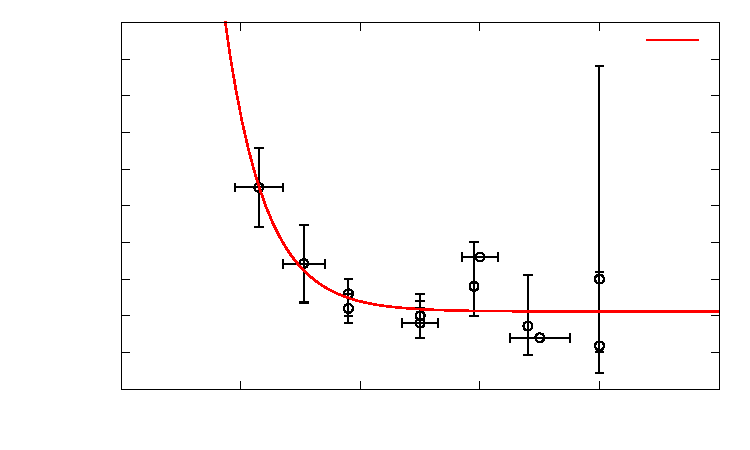
\includegraphics{GRAPH_Parameter_Fit_phi-star_exponential}}%
    \gplfronttext
  \end{picture}%
\endgroup

                        }\endgroup
                \caption{The evolution of $\phi^{*}$ as a function of redshift according to past observational studies.\label{fig:phi_evolution}}
            \end{figure}

            The final parameter is the characteristic magnitude, $M^*$. It was determined that a linear fit was best again and so the pivot method was used to reduce the error. The final equation used was $M^* = 0.221z - 21.642$.
            \begin{figure}[!htb]
                \centering
                    \begingroup\endlinechar=-1
                        \resizebox{0.6\textwidth}{!}{%
                            % GNUPLOT: LaTeX picture with Postscript
\begingroup
  \makeatletter
  \providecommand\color[2][]{%
    \GenericError{(gnuplot) \space\space\space\@spaces}{%
      Package color not loaded in conjunction with
      terminal option `colourtext'%
    }{See the gnuplot documentation for explanation.%
    }{Either use 'blacktext' in gnuplot or load the package
      color.sty in LaTeX.}%
    \renewcommand\color[2][]{}%
  }%
  \providecommand\includegraphics[2][]{%
    \GenericError{(gnuplot) \space\space\space\@spaces}{%
      Package graphicx or graphics not loaded%
    }{See the gnuplot documentation for explanation.%
    }{The gnuplot epslatex terminal needs graphicx.sty or graphics.sty.}%
    \renewcommand\includegraphics[2][]{}%
  }%
  \providecommand\rotatebox[2]{#2}%
  \@ifundefined{ifGPcolor}{%
    \newif\ifGPcolor
    \GPcolortrue
  }{}%
  \@ifundefined{ifGPblacktext}{%
    \newif\ifGPblacktext
    \GPblacktexttrue
  }{}%
  % define a \g@addto@macro without @ in the name:
  \let\gplgaddtomacro\g@addto@macro
  % define empty templates for all commands taking text:
  \gdef\gplbacktext{}%
  \gdef\gplfronttext{}%
  \makeatother
  \ifGPblacktext
    % no textcolor at all
    \def\colorrgb#1{}%
    \def\colorgray#1{}%
  \else
    % gray or color?
    \ifGPcolor
      \def\colorrgb#1{\color[rgb]{#1}}%
      \def\colorgray#1{\color[gray]{#1}}%
      \expandafter\def\csname LTw\endcsname{\color{white}}%
      \expandafter\def\csname LTb\endcsname{\color{black}}%
      \expandafter\def\csname LTa\endcsname{\color{black}}%
      \expandafter\def\csname LT0\endcsname{\color[rgb]{1,0,0}}%
      \expandafter\def\csname LT1\endcsname{\color[rgb]{0,1,0}}%
      \expandafter\def\csname LT2\endcsname{\color[rgb]{0,0,1}}%
      \expandafter\def\csname LT3\endcsname{\color[rgb]{1,0,1}}%
      \expandafter\def\csname LT4\endcsname{\color[rgb]{0,1,1}}%
      \expandafter\def\csname LT5\endcsname{\color[rgb]{1,1,0}}%
      \expandafter\def\csname LT6\endcsname{\color[rgb]{0,0,0}}%
      \expandafter\def\csname LT7\endcsname{\color[rgb]{1,0.3,0}}%
      \expandafter\def\csname LT8\endcsname{\color[rgb]{0.5,0.5,0.5}}%
    \else
      % gray
      \def\colorrgb#1{\color{black}}%
      \def\colorgray#1{\color[gray]{#1}}%
      \expandafter\def\csname LTw\endcsname{\color{white}}%
      \expandafter\def\csname LTb\endcsname{\color{black}}%
      \expandafter\def\csname LTa\endcsname{\color{black}}%
      \expandafter\def\csname LT0\endcsname{\color{black}}%
      \expandafter\def\csname LT1\endcsname{\color{black}}%
      \expandafter\def\csname LT2\endcsname{\color{black}}%
      \expandafter\def\csname LT3\endcsname{\color{black}}%
      \expandafter\def\csname LT4\endcsname{\color{black}}%
      \expandafter\def\csname LT5\endcsname{\color{black}}%
      \expandafter\def\csname LT6\endcsname{\color{black}}%
      \expandafter\def\csname LT7\endcsname{\color{black}}%
      \expandafter\def\csname LT8\endcsname{\color{black}}%
    \fi
  \fi
  \setlength{\unitlength}{0.0500bp}%
  \begin{picture}(7200.00,4320.00)%
    \gplgaddtomacro\gplbacktext{%
      \put(849,595){\makebox(0,0)[r]{\strut{}-22}}%
      \put(849,1098){\makebox(0,0)[r]{\strut{}-21.5}}%
      \put(849,1601){\makebox(0,0)[r]{\strut{}-21}}%
      \put(849,2104){\makebox(0,0)[r]{\strut{}-20.5}}%
      \put(849,2606){\makebox(0,0)[r]{\strut{}-20}}%
      \put(849,3109){\makebox(0,0)[r]{\strut{}-19.5}}%
      \put(849,3612){\makebox(0,0)[r]{\strut{}-19}}%
      \put(849,4115){\makebox(0,0)[r]{\strut{}-18.5}}%
      \put(951,409){\makebox(0,0){\strut{} 0}}%
      \put(2139,409){\makebox(0,0){\strut{} 2}}%
      \put(3328,409){\makebox(0,0){\strut{} 4}}%
      \put(4516,409){\makebox(0,0){\strut{} 6}}%
      \put(5705,409){\makebox(0,0){\strut{} 8}}%
      \put(6893,409){\makebox(0,0){\strut{} 10}}%
      \csname LTb\endcsname%
      \put(144,2355){\rotatebox{-270}{\makebox(0,0){\strut{}Characteristic Magnitude ($M^*$)}}}%
      \csname LTb\endcsname%
      \put(3922,130){\makebox(0,0){\strut{}Redshift ($z$)}}%
      \put(3922,4022){\makebox(0,0){\strut{}}}%
    }%
    \gplgaddtomacro\gplfronttext{%
      \csname LTb\endcsname%
      \put(3399,3948){\makebox(0,0)[r]{\strut{}$f(x) = 0.221x + -21.642$}}%
    }%
    \gplbacktext
    \put(0,0){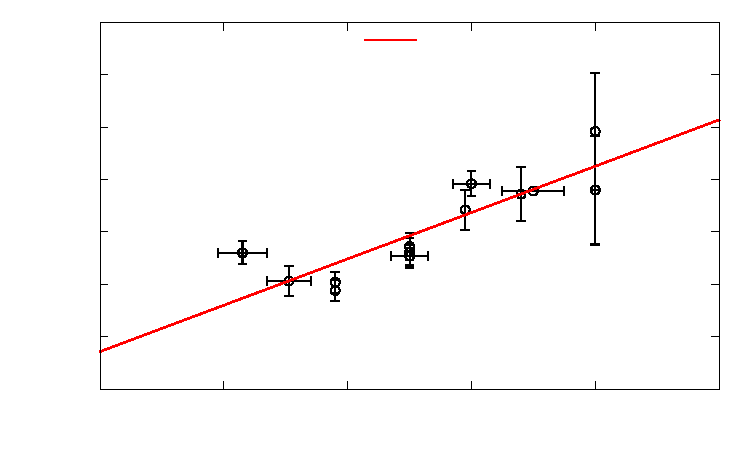
\includegraphics{GRAPH_Parameter_Fit_m-star_linear}}%
    \gplfronttext
  \end{picture}%
\endgroup

                        }\endgroup
                \caption{The evolution of $M^{*}$ as a function of redshift according to past observational studies.\label{fig:phi_evolution}}
            \end{figure}
        % subsubsection linear_parameter_evolution_with_redshift (end)
% subsection parameter_evolution (end)


    % %!TEX root = mainfile.tex

\section{Determining the rate of re-ionizing photons} % (fold)
\label{sec:determining_the_rate_of_re_ionizing_photons}
	When calculating the rate of re-ionizing photons, there are two important constants to be considered. These are the escape fraction of photons emitted by young stars which manage to escape from the galaxy, $f_\text{esc}$, and the number of hydrogen ionizing photons produced per second per unit star formation rate, $\zeta$. For the purposes of this project we will be using well established values nevertheless it is still important to understand how these values are obtained.

	\subsection{Escape Fraction} % (fold)
	\label{sub:escape_fraction}
		This value is the escape fraction of photons. If this number were one then every single photon that’s produced would escape from the galaxy into the IGM to contribute to the ionization of the neutral hydrogen however this is not the case. This figure is in fact much smaller meaning that most of the photons never reach the IGM at all. This is due to the neutral hydrogen within the galaxy itself absorbing the photons before they can escape. The amount of neutral hydrogen, the density and size of the galaxy and whether or not the galaxy is part of a cluster all contribute to the value of fesc and hence it is notoriously difficult to determine.

		It is often obtained by measuring the flux of UV photons below the Lyman limit of 912\AA which emerge from galaxies using methods such as intrepid spectroscopic and narrow-band imaging\cite{robertson2010early}. This is because only a certain fraction of the photons that were produced do emerge having managed to avoid interaction with the neutral gas within the galaxy thus measuring this flux directly and making assumptions of how many were initially produced would result in an estimate of the escape fraction. This comes with its own difficulties as often those photons which have managed to escape the galaxy are further absorbed by the IGM along the line of sight, reducing the flux that can be observed. As this method relies on observations it has not been possible to determine the escape value for high redshift galaxies and so it has been assumed that the number obtained from observations of lower redshift galaxies is approximately consistent at earlier cosmic times. As this value is so difficult to determine and varies from galaxy to galaxy it hasn’t been confirmed but instead has been constrained so hence this project will trial a range of these values to see how this can affect the rate of re-ionizing photons. Robertson et al.’s 2010 paper estimates this value to lie within the range $0.1\lesssim f_\text{esc}\lesssim 0.2$\cite{robertson2010early} whereas Inoue (2006) claims that ``fesc increases from a value less than 0.01 at $z\le1$ to about 0.1 at $z\ge 4$''\cite{inoue2006escape}. This contradicts the assumption that the escape fraction doesn’t alter with redshift however the approximate range of this value is what is required for this project not necessarily its evolution with time. Furthermore there isn’t enough data available to determine this to a great deal of accuracy and hence the extrapolated value for the escape fraction at high redshifts would be an approximation. As the value for the escape fraction can only vary from 0 to 1 its exact value cannot greatly alter the outcome of the calculation and thus an approximate value is sufficient within the realms of this project.

		The escape fraction can also be determined using galaxy formation simulations which is exactly what was done by Wood and Loeb in 2000. They found that the escape fraction at $z\approx 10$ is $\le1$\% for stars\cite{gnedin2008escape}. Calculating the escape fraction of ionizing photons from disk galaxies as a function of galaxy mass and redshift requires a complex code and that certain assumptions be made. These are that the gas in the disks is isothermal and radially exponential and that the source of radiation is either the stars within the disks or a central quasar. The mechanics of the program extend well beyond the scope of this project however the outcome of $f_\text{esc}=0.01$ is of use. As this particular paper was published in 2000 and has made relatively idealistic assumptions its legitimacy nowadays can be questioned. Therefore for the purposes of this project the observed values of $f_\text{esc}\approx 0.1$ have been used.
	% subsection escape_fraction (end)

	\subsection{Hydrogen Ionizing Photons Produced per Second per Unit Star Formation Rate} % (fold)
	\label{sub:hydrogen_ionizing_photons_produced_per_second_per_unit_star_formation_rate}
		The number of hydrogen ionizing photons produced per second per unit star formation rate is a very difficult number to pinpoint as it is not obvious how it could be determined numerically or observationally. This is because it is heavily dependent upon the characteristics of the star and, as each star is unique and stars themselves are so numerous, this becomes a very complex situation to simulate and thus it is common to take a representative average value for $\zeta$. Furthermore at the high redshifts considered in this project the stars are so far away that much bigger objects such as galaxies must instead be observed making it near-enough impossible to establish the activity of a single star.

		For the purposes of this project it has been assumed that $\zeta=10^{53.5}$\si{s^{-1}.M_{\odot}^{-1}.yr^{-1}}\cite{robertson2010early}. This particular value has been realised through the same detection methods as the escape fraction however as with fesc its precise value remains uncertain.

		The value for $\zeta$ can also be obtained numerically; more detail is included in Schull’s 2011 paper\cite{shull2012critical}. This applies a very complicated method however it essentially converts the star formation rate density into numbers of OB sequence stars and computes the total number of ionizing photons produced by a star of a certain mass over its lifetime. Combining this with the rate at which stars of this mass are formed would give a good estimate for $\zeta$. As this method is highly complex it is not clear to what extent it relates to the specifics of this project and hence although it is a highly advanced way of calculating $\zeta$ it is perhaps more sensible for the value obtained in Robertson to be used as this is a very common and better understood figure.
	% subsection hydrogen_ionizing_photons_produced_per_second_per_unit_star_formation_rate (end)
% section determining_the_rate_of_re_ionizing_photons (end)


    %!TEX root = mainfile.tex

\section{Lower Redshift limit on Re-ionization} % (fold)
\label{sec:lower_redshift_limit_on_Re-ionization}
	In the project the way that the lower redshift limit has been calculated is to first calculate the rate of photons capable of ionizing a hydrogen atom via equation~(\ref{eq:rate_of_ionising_photons})\cite{2010Natur.468...49R}.
	\begin{align}
		\frac{\d{n_{ion}}}{\d{t}}=f_{esc}\zeta\rho_\text{SFR}\label{eq:rate_of_ionising_photons}
	\end{align}
	Where $f_{esc}$ is the fraction of ionizing photons that escape a galaxy, $\zeta$ is the number of hydrogen-ionizing photons produced per second per unit star formation rate, see Section~\ref{sub:reionization_parameters}, and $\rho_\text{SFR}$ is the star formation rate per unit volume.

	Therefore by integrating this equation up to the age of the universe at a specific redshift a total number of photons capable of ionizing the universe can be outputted. The number of ionizing photons are then equated to the total number of hydrogen atoms in the IGM of the universe to obtain a lower redshift limit of reionization.

	First of all the program calculates the critical density of the universe by,
	\begin{align}
		\rho_{crit}(z)=\frac{3H{(z)}^{2}}{8\pi G}
	\end{align}
	Then by multiplying this by the baryonic density parameter, $\Omega_{b}=0.045\pm0.004$, the baryonic density is achieved. Then, by multiplying by the fraction of hydrogen, calculated from big bang nucleosynthesis, the total density of hydrogen in the universe can be obtained.

	From the 7 year WMAP survey\cite{2011ApJS..192...18K}, the primordial Helium fraction was found to be $Y=0.33\pm0.09$. Where it is assumed that Hydrogen fraction ($X$) is simply $1-Y$ (therefore 0 metallicity). Nevertheless as a simplifying assumption it is not too bad as the errors on fraction of helium are higher than the actual fraction of heavier elements.

	Then finally dividing the mass density of hydrogen by the atomic mass unit the code obtains a number density of hydrogen. In the code a redshift time relation $\frac{1}{(1+z)}\propto t^{2/3}$, assuming a matter dominated universe, is used and therefore,
	\begin{align}
		t &= \frac{t_{0}}{{(1+z)}^{3/2}} \\
		\Rightarrow \dx{t}{z} &= \frac{3}{2}\frac{t_{0}}{{(1+z)}^{5/2}}
	\end{align}

	In the first version of the code, values of star formation rate densities from  various articles with redshifts varying from redshifts 4 to up to about 8 from\cite{2010MNRAS.401.2561W}, which determine star formation rates from observations of Gamma-ray bursts (GRBs) from deaths of massive short lived stars which can be directly related to star formation rate. Also compiling these values with those from\cite{2012ApJ...759L..38A}, which use a semi-analytical model to determine star formation rates from redshifts 9 to 16. These two papers with very different methods have surprising correlation in values.

	These values were then plotted against redshift. The function of redshift that was used for $\rho_\text{SFR}$ was
	\begin{align}
		\rho_\text{SFR}(z)=0.399(\pm 0.181)\e{-0.253(\pm 0.118)z}-0.011(\pm 0.025)
	\end{align}
	However this equation only works up to a redshift of around 5 as the star formation rate for galaxies drops with redshifts lower than this due to the gas being used up and star formation dropping off. This should not effect the results too much however as the project tends to study redshifts higher than this anyway. Also there are be large errors on higher redshift values due to problems with extrapolating the data, and unrealistic numbers of star formation where in reality there would be none. The values of $f_\text{esc}=0.2$ and $\zeta=10^{53.5}$ as stated in sections~\ref{sub:escape_fraction} and~\ref{sub:hydrogen_ionizing_photons_produced_per_second_per_unit_star_formation_rate} were applied here.

	The code also used a function of the global stellar mass density to figure out the amount of hydrogen that was calculated was in stars at a given redshift. This therefore gives a certain fraction that is not part of the IGM and does not need to be ionized. These values were taken from the direct observations of three papers \cite{2006AA...459..745F}, \cite{2003A&A...401...73W} and \cite{2003ApJS..149..289B}. The function of redshift that was calculated was
	\begin{align}
		\rho_\text{stellar}(M_{\odot}\si{\per\mega\parsec\cubed})=\e{-0.81z+19.7}
	\end{align}
	but this does not have much effect on the number of hydrogen as the stellar fraction is very small, so this is not a significant contributing factor.

	The code then loops for different values of redshift from redshift 25 at redshift intervals of 0.1, calculating the number of ionizing photons at those different epochs and equating this to the hydrogen number. This then outputs ionized fraction against redshift, shown in Figure~\ref{fig:IonizedFraction1}.
	\begin{figure}[htbp]
		\centering
			\begingroup\endlinechar=-1
		  		\resizebox{0.7\textwidth}{!}{%
					% GNUPLOT: LaTeX picture with Postscript
\begingroup
  \makeatletter
  \providecommand\color[2][]{%
    \GenericError{(gnuplot) \space\space\space\@spaces}{%
      Package color not loaded in conjunction with
      terminal option `colourtext'%
    }{See the gnuplot documentation for explanation.%
    }{Either use 'blacktext' in gnuplot or load the package
      color.sty in LaTeX.}%
    \renewcommand\color[2][]{}%
  }%
  \providecommand\includegraphics[2][]{%
    \GenericError{(gnuplot) \space\space\space\@spaces}{%
      Package graphicx or graphics not loaded%
    }{See the gnuplot documentation for explanation.%
    }{The gnuplot epslatex terminal needs graphicx.sty or graphics.sty.}%
    \renewcommand\includegraphics[2][]{}%
  }%
  \providecommand\rotatebox[2]{#2}%
  \@ifundefined{ifGPcolor}{%
    \newif\ifGPcolor
    \GPcolortrue
  }{}%
  \@ifundefined{ifGPblacktext}{%
    \newif\ifGPblacktext
    \GPblacktexttrue
  }{}%
  % define a \g@addto@macro without @ in the name:
  \let\gplgaddtomacro\g@addto@macro
  % define empty templates for all commands taking text:
  \gdef\gplbacktext{}%
  \gdef\gplfronttext{}%
  \makeatother
  \ifGPblacktext
    % no textcolor at all
    \def\colorrgb#1{}%
    \def\colorgray#1{}%
  \else
    % gray or color?
    \ifGPcolor
      \def\colorrgb#1{\color[rgb]{#1}}%
      \def\colorgray#1{\color[gray]{#1}}%
      \expandafter\def\csname LTw\endcsname{\color{white}}%
      \expandafter\def\csname LTb\endcsname{\color{black}}%
      \expandafter\def\csname LTa\endcsname{\color{black}}%
      \expandafter\def\csname LT0\endcsname{\color[rgb]{1,0,0}}%
      \expandafter\def\csname LT1\endcsname{\color[rgb]{0,1,0}}%
      \expandafter\def\csname LT2\endcsname{\color[rgb]{0,0,1}}%
      \expandafter\def\csname LT3\endcsname{\color[rgb]{1,0,1}}%
      \expandafter\def\csname LT4\endcsname{\color[rgb]{0,1,1}}%
      \expandafter\def\csname LT5\endcsname{\color[rgb]{1,1,0}}%
      \expandafter\def\csname LT6\endcsname{\color[rgb]{0,0,0}}%
      \expandafter\def\csname LT7\endcsname{\color[rgb]{1,0.3,0}}%
      \expandafter\def\csname LT8\endcsname{\color[rgb]{0.5,0.5,0.5}}%
    \else
      % gray
      \def\colorrgb#1{\color{black}}%
      \def\colorgray#1{\color[gray]{#1}}%
      \expandafter\def\csname LTw\endcsname{\color{white}}%
      \expandafter\def\csname LTb\endcsname{\color{black}}%
      \expandafter\def\csname LTa\endcsname{\color{black}}%
      \expandafter\def\csname LT0\endcsname{\color{black}}%
      \expandafter\def\csname LT1\endcsname{\color{black}}%
      \expandafter\def\csname LT2\endcsname{\color{black}}%
      \expandafter\def\csname LT3\endcsname{\color{black}}%
      \expandafter\def\csname LT4\endcsname{\color{black}}%
      \expandafter\def\csname LT5\endcsname{\color{black}}%
      \expandafter\def\csname LT6\endcsname{\color{black}}%
      \expandafter\def\csname LT7\endcsname{\color{black}}%
      \expandafter\def\csname LT8\endcsname{\color{black}}%
    \fi
  \fi
  \setlength{\unitlength}{0.0500bp}%
  \begin{picture}(7200.00,4320.00)%
    \gplgaddtomacro\gplbacktext{%
      \put(747,595){\makebox(0,0)[r]{\strut{} 0}}%
      \put(747,1182){\makebox(0,0)[r]{\strut{} 0.2}}%
      \put(747,1768){\makebox(0,0)[r]{\strut{} 0.4}}%
      \put(747,2355){\makebox(0,0)[r]{\strut{} 0.6}}%
      \put(747,2942){\makebox(0,0)[r]{\strut{} 0.8}}%
      \put(747,3528){\makebox(0,0)[r]{\strut{} 1}}%
      \put(747,4115){\makebox(0,0)[r]{\strut{} 1.2}}%
      \put(849,409){\makebox(0,0){\strut{} 0}}%
      \put(2058,409){\makebox(0,0){\strut{} 5}}%
      \put(3267,409){\makebox(0,0){\strut{} 10}}%
      \put(4475,409){\makebox(0,0){\strut{} 15}}%
      \put(5684,409){\makebox(0,0){\strut{} 20}}%
      \put(6893,409){\makebox(0,0){\strut{} 25}}%
      \csname LTb\endcsname%
      \put(144,2355){\rotatebox{-270}{\makebox(0,0){\strut{}Ionised Fraction ($X$)}}}%
      \csname LTb\endcsname%
      \put(3871,130){\makebox(0,0){\strut{}Redshift (z)}}%
      \put(3871,4022){\makebox(0,0){\strut{}}}%
    }%
    \gplgaddtomacro\gplfronttext{%
      \csname LTb\endcsname%
      \put(6105,3948){\makebox(0,0)[r]{\strut{}Best Fit}}%
      \csname LTb\endcsname%
      \put(6105,3762){\makebox(0,0)[r]{\strut{}Lower Limit}}%
      \csname LTb\endcsname%
      \put(6105,3576){\makebox(0,0)[r]{\strut{}Upper Limit}}%
    }%
    \gplbacktext
    \put(0,0){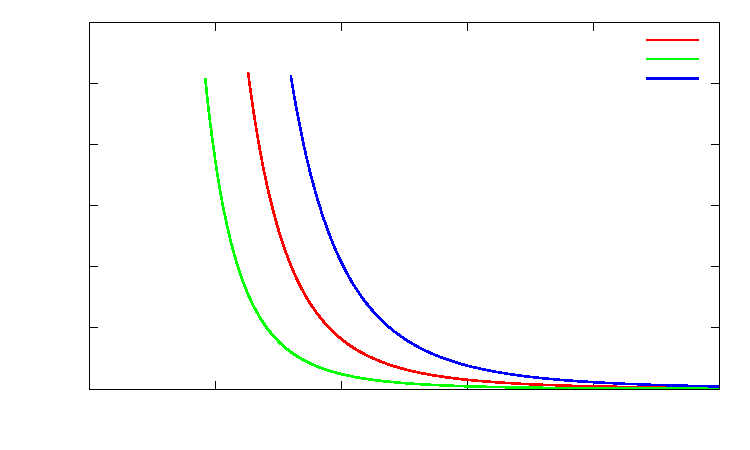
\includegraphics{GRAPH_StellarDens_exponential}}%
    \gplfronttext
  \end{picture}%
\endgroup

		  		}\endgroup
		\caption{Plot of modeled ionized fraction of the IGM as a function of redshift.\label{fig:IonizedFraction1}}
	\end{figure}

	This implies that the universe is completely ionized at a redshift $6.3\pm1.7$, ignoring the rather large errors, this number is not a bad estimate of the epoch. This is known from articles which show from observations of Lyman-$\alpha$ emitters that there must be a large ionized fraction at $z=6.5$, due to attenuation from neutral hydrogen\cite{Ota:arXiv0707.1561}. Various theoretical models of star formation rate predict a ionized universe at around $z=6$ and it is stated that the Sunyaev-Zeldovich effect has limited the end of reionization to earlier than $z=5.8$\cite{2012MNRAS.423..862K}. Therefore we have a predicted epoch of reionization of $5.8<z<6.5$ from the literature.

	However as recombination has not been included which will slow down the rate at which the universe is ionized, as it is effectively the opposite effect of reionization. Or the fact that both the escape fraction and $\zeta$ are likely to change with redshift, makes this number is not entirely realistic.

	\subsection{Reionization Parameters} % (fold)
	\label{sub:reionization_parameters}
		When calculating the rate of re-ionizing photons, there are two important constants to be considered. These are the escape fraction of photons emitted by young stars which manage to escape from the galaxy, $f_\text{esc}$, and the number of hydrogen ionizing photons produced per second per unit star formation rate, $\zeta$. Throughout this project, well established values have been used nevertheless it is still important to understand how these values are obtained.
	% subsection reionization_parameters (end)

		\subsubsection{Escape Fraction} % (fold)
		\label{sub:escape_fraction}
			This value is the escape fraction of photons. If this number were one then every single photon that's produced would escape from the galaxy into the IGM to contribute to the ionization of the neutral hydrogen however this is not the case. This figure is in fact much smaller meaning that most of the photons never reach the IGM at all. This is due to the neutral hydrogen within the galaxy itself absorbing the photons before they can escape. The amount of neutral hydrogen, the density and size of the galaxy and whether or not the galaxy is part of a cluster all contribute to the value of fesc and hence it is notoriously difficult to determine.

			It is often obtained by measuring the flux of UV photons below the Lyman limit of \SI{912}{\angstrom} which emerge from galaxies using methods such as intrepid spectroscopic and narrow-band imaging\cite{robertson2010early}. This is because only a certain fraction of the photons that were produced do emerge having managed to avoid interaction with the neutral gas within the galaxy thus measuring this flux directly and making assumptions of how many were initially produced would result in an estimate of the escape fraction. This comes with its own difficulties as often those photons which have managed to escape the galaxy are further absorbed by the IGM along the line of sight, reducing the flux that can be observed. This method relies on observations it has not been possible to determine the escape value for high redshift galaxies and so it has been extrapolated back to earlier cosmic times in Section~\ref{sub:evolving_escape_fraction}. As this value is so difficult to determine and varies from galaxy to galaxy it hasn't been confirmed but instead has been constrained so hence this project will trial a range of these values to see how this can affect the rate of re-ionizing photons. Robertson et al.'s 2010 paper estimates this value to lie within the range $0.1\lesssim f_\text{esc}\lesssim 0.2$\cite{robertson2010early} whereas Inoue (2006) claims that ``fesc increases from a value less than 0.01 at $z\le 1$ to about 0.1 at $z\ge 4$''\cite{inoue2006escape}. Furthermore there isn't enough data available to determine this to a great deal of accuracy and hence the extrapolated value for the escape fraction at high redshifts would be an approximation. As the value for the escape fraction can only vary from 0 to 1 its exact value cannot greatly alter the outcome of the calculation and thus an approximate value is sufficient within the realms of this project.

			The escape fraction can also be determined using galaxy formation simulations which is exactly what was done by Wood and Loeb in 2000. They found that the escape fraction at $z\approx 10$ is $\le1$\% for stars\cite{gnedin2008escape}. Calculating the escape fraction of ionizing photons from disk galaxies as a function of galaxy mass and redshift requires a complex code and that certain assumptions be made. These are that the gas in the disks is isothermal and radially exponential and that the source of radiation is either the stars within the disks or a central quasar. The mechanics of the program extend well beyond the scope of this project however the outcome of $f_\text{esc}=0.01$ is of use. As this particular paper was published in 2000 and has made relatively idealistic assumptions its legitimacy nowadays can be questioned. Therefore for the purposes of this project the observed values of $f_\text{esc}\approx 0.2$ were initially used with its evolution with redshift incorporated later.
		% subsection escape_fraction (end)

		\subsubsection{Hydrogen Ionizing Photons Produced ($s^{-1}M_\odot^{-1}\text{yr}$)} % (fold)
		\label{sub:hydrogen_ionizing_photons_produced_per_second_per_unit_star_formation_rate}
			The number of hydrogen ionizing photons produced per second per unit star formation rate is a very difficult number to pinpoint as it is not obvious how it could be determined numerically or observationally. This is because it is heavily dependent upon the characteristics of the star and, as each star is unique and stars themselves are so numerous, this becomes a very complex situation to simulate and thus it is common to take a representative average value for $\zeta$. Furthermore at the high redshifts considered in this project the stars are so far away that much bigger objects such as galaxies must instead be observed making it near-enough impossible to establish the activity of a single star.

			For the purposes of this project it has been assumed that $\zeta=10^{53.5}$\si{s^{-1}.M_{\odot}^{-1}.yr^{-1}}\cite{robertson2010early}. This particular value has been realised through the same detection methods as the escape fraction however as with fesc its precise value remains uncertain.

			The value for $\zeta$ can also be obtained numerically; more detail is included in Schull's 2011 paper\cite{shull2012critical}. This applies a very complicated method however it essentially converts the star formation rate density into numbers of OB sequence stars and computes the total number of ionizing photons produced by a star of a certain mass over its lifetime. Combining this with the rate at which stars of this mass are formed would give a good estimate for $\zeta$. As this method is highly complex it is not clear to what extent it relates to the specifics of this project and hence although it is a highly advanced way of calculating $\zeta$ it is perhaps more sensible for the value obtained in Robertson to be used as this is a very common and better understood figure.
		% subsection hydrogen_ionizing_photons_produced_per_second_per_unit_star_formation_rate (end)

	\subsection{Evolving Escape Fraction} % (fold)
	\label{sub:evolving_escape_fraction}
		As already stated the previous results make a basic assumption of of the escape fraction to be about $20\%$ during the epoch of reionization. This is obviously not a very good assumption as it will evolve with redshift. However there lies a problem in this which is related to the previous section, Section~\ref{sub:escape_fraction} which explained the difficulty in measuring this parameter as well as the problems in extrapolating out to higher redshifts much like in our star formation rates. This uncertainty in the measurement is what leads to the differences stated in\cite{2012ApJ...759L..38A}, which states a higher fraction at higher redshift due to lack of dust, and\cite{2000ApJ...545...86W} which states the opposite, due to increasing disk densities and increasing density in the universe as a whole. However from\cite{2012arXiv1209.2123F} and\cite{2013MNRAS.428L...1M} by using recent semi-analytical models they found that the escape fraction does indeed increase with redshift and so this is the model that is used in this project.

		Once again using the fit program to fit a exponential to the escape fraction measurements and predictions from\cite{2012ApJ...759L..38A},\cite{2006ApJ...651L..89R} and\cite{2006MNRAS.371L...1I}. The functional form that is achieved is
		\begin{align}
			f_\text{esc}(z)=\e{0.013\pm0.011-0.952\pm0.06}
		\end{align}
		The code is then run again with this escape fraction instead of the constant $20\%$, the results achieved are shown in \ref{fig:IonizedFraction2}
		\begin{figure}[htbp]
			\centering
				\begingroup\endlinechar=-1
					\resizebox{0.7\textwidth}{!}{%
						% GNUPLOT: LaTeX picture with Postscript
\begingroup
  \makeatletter
  \providecommand\color[2][]{%
    \GenericError{(gnuplot) \space\space\space\@spaces}{%
      Package color not loaded in conjunction with
      terminal option `colourtext'%
    }{See the gnuplot documentation for explanation.%
    }{Either use 'blacktext' in gnuplot or load the package
      color.sty in LaTeX.}%
    \renewcommand\color[2][]{}%
  }%
  \providecommand\includegraphics[2][]{%
    \GenericError{(gnuplot) \space\space\space\@spaces}{%
      Package graphicx or graphics not loaded%
    }{See the gnuplot documentation for explanation.%
    }{The gnuplot epslatex terminal needs graphicx.sty or graphics.sty.}%
    \renewcommand\includegraphics[2][]{}%
  }%
  \providecommand\rotatebox[2]{#2}%
  \@ifundefined{ifGPcolor}{%
    \newif\ifGPcolor
    \GPcolortrue
  }{}%
  \@ifundefined{ifGPblacktext}{%
    \newif\ifGPblacktext
    \GPblacktexttrue
  }{}%
  % define a \g@addto@macro without @ in the name:
  \let\gplgaddtomacro\g@addto@macro
  % define empty templates for all commands taking text:
  \gdef\gplbacktext{}%
  \gdef\gplfronttext{}%
  \makeatother
  \ifGPblacktext
    % no textcolor at all
    \def\colorrgb#1{}%
    \def\colorgray#1{}%
  \else
    % gray or color?
    \ifGPcolor
      \def\colorrgb#1{\color[rgb]{#1}}%
      \def\colorgray#1{\color[gray]{#1}}%
      \expandafter\def\csname LTw\endcsname{\color{white}}%
      \expandafter\def\csname LTb\endcsname{\color{black}}%
      \expandafter\def\csname LTa\endcsname{\color{black}}%
      \expandafter\def\csname LT0\endcsname{\color[rgb]{1,0,0}}%
      \expandafter\def\csname LT1\endcsname{\color[rgb]{0,1,0}}%
      \expandafter\def\csname LT2\endcsname{\color[rgb]{0,0,1}}%
      \expandafter\def\csname LT3\endcsname{\color[rgb]{1,0,1}}%
      \expandafter\def\csname LT4\endcsname{\color[rgb]{0,1,1}}%
      \expandafter\def\csname LT5\endcsname{\color[rgb]{1,1,0}}%
      \expandafter\def\csname LT6\endcsname{\color[rgb]{0,0,0}}%
      \expandafter\def\csname LT7\endcsname{\color[rgb]{1,0.3,0}}%
      \expandafter\def\csname LT8\endcsname{\color[rgb]{0.5,0.5,0.5}}%
    \else
      % gray
      \def\colorrgb#1{\color{black}}%
      \def\colorgray#1{\color[gray]{#1}}%
      \expandafter\def\csname LTw\endcsname{\color{white}}%
      \expandafter\def\csname LTb\endcsname{\color{black}}%
      \expandafter\def\csname LTa\endcsname{\color{black}}%
      \expandafter\def\csname LT0\endcsname{\color{black}}%
      \expandafter\def\csname LT1\endcsname{\color{black}}%
      \expandafter\def\csname LT2\endcsname{\color{black}}%
      \expandafter\def\csname LT3\endcsname{\color{black}}%
      \expandafter\def\csname LT4\endcsname{\color{black}}%
      \expandafter\def\csname LT5\endcsname{\color{black}}%
      \expandafter\def\csname LT6\endcsname{\color{black}}%
      \expandafter\def\csname LT7\endcsname{\color{black}}%
      \expandafter\def\csname LT8\endcsname{\color{black}}%
    \fi
  \fi
  \setlength{\unitlength}{0.0500bp}%
  \begin{picture}(7200.00,4320.00)%
    \gplgaddtomacro\gplbacktext{%
      \put(747,595){\makebox(0,0)[r]{\strut{} 0}}%
      \put(747,1235){\makebox(0,0)[r]{\strut{} 0.2}}%
      \put(747,1875){\makebox(0,0)[r]{\strut{} 0.4}}%
      \put(747,2515){\makebox(0,0)[r]{\strut{} 0.6}}%
      \put(747,3155){\makebox(0,0)[r]{\strut{} 0.8}}%
      \put(747,3795){\makebox(0,0)[r]{\strut{} 1}}%
      \put(849,409){\makebox(0,0){\strut{} 4}}%
      \put(1398,409){\makebox(0,0){\strut{} 6}}%
      \put(1948,409){\makebox(0,0){\strut{} 8}}%
      \put(2497,409){\makebox(0,0){\strut{} 10}}%
      \put(3047,409){\makebox(0,0){\strut{} 12}}%
      \put(3596,409){\makebox(0,0){\strut{} 14}}%
      \put(4146,409){\makebox(0,0){\strut{} 16}}%
      \put(4695,409){\makebox(0,0){\strut{} 18}}%
      \put(5245,409){\makebox(0,0){\strut{} 20}}%
      \put(5794,409){\makebox(0,0){\strut{} 22}}%
      \put(6344,409){\makebox(0,0){\strut{} 24}}%
      \put(6893,409){\makebox(0,0){\strut{} 26}}%
      \csname LTb\endcsname%
      \put(144,2355){\rotatebox{-270}{\makebox(0,0){\strut{}Ionised Fraction}}}%
      \csname LTb\endcsname%
      \put(3871,130){\makebox(0,0){\strut{}Redshift ($z$)}}%
      \put(3871,4022){\makebox(0,0){\strut{}}}%
    }%
    \gplgaddtomacro\gplfronttext{%
      \csname LTb\endcsname%
      \put(5658,3702){\makebox(0,0)[r]{\strut{}Ionised Fraction}}%
      \csname LTb\endcsname%
      \put(5658,3516){\makebox(0,0)[r]{\strut{}Upper Limit}}%
      \csname LTb\endcsname%
      \put(5658,3330){\makebox(0,0)[r]{\strut{}Lower Limit}}%
    }%
    \gplbacktext
    \put(0,0){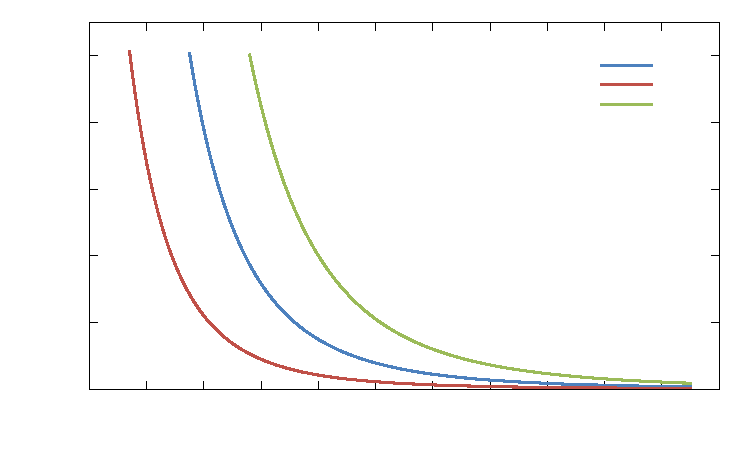
\includegraphics{GRAPH_SFR_ionised_fraction}}%
    \gplfronttext
  \end{picture}%
\endgroup

					}\endgroup
			\caption{Plot of modeled ionized fraction of the IGM as a function of redshift with predicting evolving escape fraction.\label{fig:IonizedFraction2}}
		\end{figure}

		The graph in Figure~\ref{fig:IonizedFraction2} shows that the addition of the evolving escape fraction has resulted in the universe being ionized quicker which is what is expected, since recombinations have not been included in this model. This model outputs a redshift of $7.5\pm2.1$, which shows the increase in redshift and also in error due to the error on $f_\text{esc}$ itself. It is very hard to determine whether this is an improvement or a hindrance to the previous model just due to the uncertainty on measuring/predicting $f_\text{esc}$, therefore it is hard to be certain of accuracy of the evolving form of $f_\text{esc}$.
	% subsection evolving_escape_fraction (end)

	% \subsection{Recombinations} % (fold)
	% \label{sub:recombinations}
	% %Not completed having trouble with it not sure if it should be included without conclusive results?
	% 	To include Recombinations into our project, the rate at which hydrogen will recombine. The recombination rate was found to be,
	% 	\begin{align}
	% 		\frac{dn_{rec}}{dt}=\frac{Q_{HII}}{\overline{t}_{rec}}
	% 	\end{align}
	% 	Where $\overline{t}_\text{rec}$ is the mean recombination time and $Q_\text{HII}$ is the ``volume filling factor''\cite{2012ApJ...746..125H}. The mean recombination time has the form,
	% 	\begin{align}
	% 		\overline{t}_{rec}= {\left(1.08\langle n_{H}\rangle\alpha_{B}C\right)}^{-1}
	% 	\end{align}
	% 	Where $C$ is the clumping factor the IGM, $\alpha_{B}$ is the recombination coefficent for excited states of hydrogen and the 1.08 accounts for the presence of photoelectrons from singly ionized helium. Where values of the clumping factor against redshift are cited from a theoretical model in\cite{2011MNRAS.412L..16R}.

	% 	The code then takes this equation for the mean recombination time of hydrogen and integrates the inverse of this from 0 to the specific $t(z)$. This will give us a mean total of hydrogen that will have recombined in that time period. However when this method is implemented into the code and ran, it outputs values of recombination that are insignificant because they are so low. This seems unphysical as we would expect the recombinations in the universe to be much higher than this and make a significant contribution to the rate at which the universe ionizes.
	% % subsection recombinations (end)

% section lower_redshift_limit_on_reionization (end)

        %!TEX root = mainfile.tex

\subsection{Including Recombinations} % (fold)
\label{sub:including_recombinations}

	To include Recombinations into our project, the rate at which hydrogen will recombine. The mean recombination time\cite{2012ApJ...746..125H} has the form
	\begin{align}
		\overline{t}_\text{rec}= \left[1.08\langle n_{H}\rangle\alpha_{B}C \right]^{-1}
	\end{align}
	Where $C$ is the clumping factor of the IGM (Section~\ref{sec:clumping_factor}), $\alpha_{B}$ is the recombination coefficent for excited states of hydrogen and the 1.08 accounts for the presence of photoelectrons from singly ionized helium.

	Values of the clumping factor against redshift are the ones used in Section~\ref{sec:clumping_factor}. The recombination coefficient for excited hydrogen is cited from\cite{1993PhyA..192..249L} and is proportional to $T_\text{IGM}^{-0.7}$ and at $T_\text{IGM}= 10^{4}$K it is equal to $2.6\times 10^{-13}$, therefore it is computed in the code as
	\begin{align}
		\alpha_{B}(T)(\si{\cubic\centi\metre\per\second}) &= \frac{2.6\times 10^{-13}*(10^{4})^{0.7}}{T^{0.7}}
	\end{align}
	However this also needs to be converted to \si{\cubic\mega\parsec} therefore we divide this equation by $(3.086\times 10^{24})^{3}$. Where the temperature of the IGM relation with redshift, derived from models\cite{2006MNRAS.373.1265O}, is
	\begin{align}
		T(z)=70047z^{-1.209}
	\end{align}
	To convert this into a rate of recombinations the code treats the recombinations as decays from hydrogen ionized state, with a lifetime of the mean recombination time. Then using the universal decay law the number of recombinations at a time, $t$, is
	\begin{align}
		n_{rec}(t)=n_\text{ion}(t)*\e{-t/\overline{t}_{rec}(t)}
	\end{align}
	Where we are taking $n_\text{ion}(t)$ to be the number of ionized hydrogen atoms at the time $t$. The code then does as it did in the previous cases but this time the fraction is
	\begin{align}
		X(z)=\frac{n_{ion}(z)-n_{rec}(z)}{n_{H}(z)}
	\end{align}
	This new outputted data is shown in figure \ref{fig:IonizedFraction3}.
	\begin{figure}[!htbp]
		\centering
			\begingroup\endlinechar=-1
				\resizebox{0.7\textwidth}{!}{%
					% GNUPLOT: LaTeX picture with Postscript
\begingroup
  \makeatletter
  \providecommand\color[2][]{%
    \GenericError{(gnuplot) \space\space\space\@spaces}{%
      Package color not loaded in conjunction with
      terminal option `colourtext'%
    }{See the gnuplot documentation for explanation.%
    }{Either use 'blacktext' in gnuplot or load the package
      color.sty in LaTeX.}%
    \renewcommand\color[2][]{}%
  }%
  \providecommand\includegraphics[2][]{%
    \GenericError{(gnuplot) \space\space\space\@spaces}{%
      Package graphicx or graphics not loaded%
    }{See the gnuplot documentation for explanation.%
    }{The gnuplot epslatex terminal needs graphicx.sty or graphics.sty.}%
    \renewcommand\includegraphics[2][]{}%
  }%
  \providecommand\rotatebox[2]{#2}%
  \@ifundefined{ifGPcolor}{%
    \newif\ifGPcolor
    \GPcolortrue
  }{}%
  \@ifundefined{ifGPblacktext}{%
    \newif\ifGPblacktext
    \GPblacktexttrue
  }{}%
  % define a \g@addto@macro without @ in the name:
  \let\gplgaddtomacro\g@addto@macro
  % define empty templates for all commands taking text:
  \gdef\gplbacktext{}%
  \gdef\gplfronttext{}%
  \makeatother
  \ifGPblacktext
    % no textcolor at all
    \def\colorrgb#1{}%
    \def\colorgray#1{}%
  \else
    % gray or color?
    \ifGPcolor
      \def\colorrgb#1{\color[rgb]{#1}}%
      \def\colorgray#1{\color[gray]{#1}}%
      \expandafter\def\csname LTw\endcsname{\color{white}}%
      \expandafter\def\csname LTb\endcsname{\color{black}}%
      \expandafter\def\csname LTa\endcsname{\color{black}}%
      \expandafter\def\csname LT0\endcsname{\color[rgb]{1,0,0}}%
      \expandafter\def\csname LT1\endcsname{\color[rgb]{0,1,0}}%
      \expandafter\def\csname LT2\endcsname{\color[rgb]{0,0,1}}%
      \expandafter\def\csname LT3\endcsname{\color[rgb]{1,0,1}}%
      \expandafter\def\csname LT4\endcsname{\color[rgb]{0,1,1}}%
      \expandafter\def\csname LT5\endcsname{\color[rgb]{1,1,0}}%
      \expandafter\def\csname LT6\endcsname{\color[rgb]{0,0,0}}%
      \expandafter\def\csname LT7\endcsname{\color[rgb]{1,0.3,0}}%
      \expandafter\def\csname LT8\endcsname{\color[rgb]{0.5,0.5,0.5}}%
    \else
      % gray
      \def\colorrgb#1{\color{black}}%
      \def\colorgray#1{\color[gray]{#1}}%
      \expandafter\def\csname LTw\endcsname{\color{white}}%
      \expandafter\def\csname LTb\endcsname{\color{black}}%
      \expandafter\def\csname LTa\endcsname{\color{black}}%
      \expandafter\def\csname LT0\endcsname{\color{black}}%
      \expandafter\def\csname LT1\endcsname{\color{black}}%
      \expandafter\def\csname LT2\endcsname{\color{black}}%
      \expandafter\def\csname LT3\endcsname{\color{black}}%
      \expandafter\def\csname LT4\endcsname{\color{black}}%
      \expandafter\def\csname LT5\endcsname{\color{black}}%
      \expandafter\def\csname LT6\endcsname{\color{black}}%
      \expandafter\def\csname LT7\endcsname{\color{black}}%
      \expandafter\def\csname LT8\endcsname{\color{black}}%
    \fi
  \fi
  \setlength{\unitlength}{0.0500bp}%
  \begin{picture}(7200.00,4320.00)%
    \gplgaddtomacro\gplbacktext{%
      \put(747,595){\makebox(0,0)[r]{\strut{} 0}}%
      \put(747,1182){\makebox(0,0)[r]{\strut{} 0.2}}%
      \put(747,1768){\makebox(0,0)[r]{\strut{} 0.4}}%
      \put(747,2355){\makebox(0,0)[r]{\strut{} 0.6}}%
      \put(747,2942){\makebox(0,0)[r]{\strut{} 0.8}}%
      \put(747,3528){\makebox(0,0)[r]{\strut{} 1}}%
      \put(747,4115){\makebox(0,0)[r]{\strut{} 1.2}}%
      \put(849,409){\makebox(0,0){\strut{} 6}}%
      \put(1453,409){\makebox(0,0){\strut{} 8}}%
      \put(2058,409){\makebox(0,0){\strut{} 10}}%
      \put(2662,409){\makebox(0,0){\strut{} 12}}%
      \put(3267,409){\makebox(0,0){\strut{} 14}}%
      \put(3871,409){\makebox(0,0){\strut{} 16}}%
      \put(4475,409){\makebox(0,0){\strut{} 18}}%
      \put(5080,409){\makebox(0,0){\strut{} 20}}%
      \put(5684,409){\makebox(0,0){\strut{} 22}}%
      \put(6289,409){\makebox(0,0){\strut{} 24}}%
      \put(6893,409){\makebox(0,0){\strut{} 26}}%
      \csname LTb\endcsname%
      \put(144,2355){\rotatebox{-270}{\makebox(0,0){\strut{}Ionized Fraction}}}%
      \csname LTb\endcsname%
      \put(3871,130){\makebox(0,0){\strut{}Redshift ($z$)}}%
      \put(3871,4022){\makebox(0,0){\strut{}}}%
    }%
    \gplgaddtomacro\gplfronttext{%
      \csname LTb\endcsname%
      \put(5603,3729){\makebox(0,0)[r]{\strut{}Best Fit}}%
      \csname LTb\endcsname%
      \put(5603,3543){\makebox(0,0)[r]{\strut{}Lower Limit}}%
      \csname LTb\endcsname%
      \put(5603,3357){\makebox(0,0)[r]{\strut{}Upper Limit}}%
    }%
    \gplbacktext
    \put(0,0){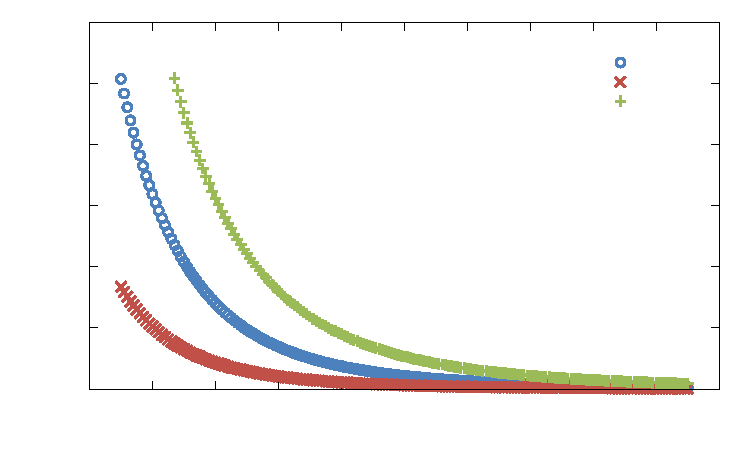
\includegraphics{GRAPH_recombinations}}%
    \gplfronttext
  \end{picture}%
\endgroup

				}\endgroup
		\caption{Ionized Fraction against redshift with recombinations and escape fraction included\label{fig:IonizedFraction3}}
	\end{figure}
	Which gives a redshift value of $7\pm1.8$ when fully ionized. This is still higher redshift than what we would expect it to be from the literature. This is probably mainly due to the large errors in value of the evolving escape fraction. Although it would appear that the first model is the most accurate in this regard it is not a very realistic number due to oversimplifying assumptions made.

	%talk about results
% subsection including_recombinations (end)




    %!TEX root = mainfile.tex

\newpage
\section{Calculating the timescale of Reionization} % (fold)
\label{sec:calculating_the_timescale_of_reionization}

	In the ``dark ages'' of the universe, when the universe had cooled, and matter had recombined to form neutral hydrogen, the temperature was not high enough to excite either hydrogen or helium out of the ground state, and consequently neither cooled effectively via atomic line emission. Thus no photon had sufficient energy to ionize neutral hydrogen.

	As stars began forming, the internal temperature of the gas was high enough for atomic line emission to occur, and ionizing photons were produced. At a particular redshift the star formation rate density was great enough to overcome the recombination rate. The star formation rate density at this point corresponds to the \emph{critical star formation rate density}. The star formation rate decreases with redshift, and conversely, the critical star formation rate increases, due to it proportionality with the clumping factor, Section~\ref{sec:clumping_factor}.

	\subsection{Critical Star Formation Rate Density} % (fold)
	\label{sub:critical_star_formation_rate_density}
		The critical star formation rate density was found by an analytical model, given by the following formula\cite{Pawlik:2009ij}.
		\begin{align}
			\rho^*_\text{SFR} = 0.027 \times f^{-1}_\text{esc} \left (\frac{C}{30} \right ) \left (\frac{1+z}{7} \right )^3 \left (\frac{\Omega_b h^2}{0.0465} \right )^2 (M_\odot \text{yr}^{-1} \text{Mpc}^{-3})
		\end{align}
		where $z$ is the redshift, $\Omega_b$ is the baryonic mass density and $C$ is the clumping factor. The graph of $\rho^*_\text{SFR}$ was plotted see Figure~\ref{fig:GRAPH_SFR_Density}.
		\begin{figure}[htbp]
			\centering
				\begingroup\endlinechar=-1
					\resizebox{0.8\textwidth}{!}{%
						% GNUPLOT: LaTeX picture with Postscript
\begingroup
  \makeatletter
  \providecommand\color[2][]{%
    \GenericError{(gnuplot) \space\space\space\@spaces}{%
      Package color not loaded in conjunction with
      terminal option `colourtext'%
    }{See the gnuplot documentation for explanation.%
    }{Either use 'blacktext' in gnuplot or load the package
      color.sty in LaTeX.}%
    \renewcommand\color[2][]{}%
  }%
  \providecommand\includegraphics[2][]{%
    \GenericError{(gnuplot) \space\space\space\@spaces}{%
      Package graphicx or graphics not loaded%
    }{See the gnuplot documentation for explanation.%
    }{The gnuplot epslatex terminal needs graphicx.sty or graphics.sty.}%
    \renewcommand\includegraphics[2][]{}%
  }%
  \providecommand\rotatebox[2]{#2}%
  \@ifundefined{ifGPcolor}{%
    \newif\ifGPcolor
    \GPcolortrue
  }{}%
  \@ifundefined{ifGPblacktext}{%
    \newif\ifGPblacktext
    \GPblacktexttrue
  }{}%
  % define a \g@addto@macro without @ in the name:
  \let\gplgaddtomacro\g@addto@macro
  % define empty templates for all commands taking text:
  \gdef\gplbacktext{}%
  \gdef\gplfronttext{}%
  \makeatother
  \ifGPblacktext
    % no textcolor at all
    \def\colorrgb#1{}%
    \def\colorgray#1{}%
  \else
    % gray or color?
    \ifGPcolor
      \def\colorrgb#1{\color[rgb]{#1}}%
      \def\colorgray#1{\color[gray]{#1}}%
      \expandafter\def\csname LTw\endcsname{\color{white}}%
      \expandafter\def\csname LTb\endcsname{\color{black}}%
      \expandafter\def\csname LTa\endcsname{\color{black}}%
      \expandafter\def\csname LT0\endcsname{\color[rgb]{1,0,0}}%
      \expandafter\def\csname LT1\endcsname{\color[rgb]{0,1,0}}%
      \expandafter\def\csname LT2\endcsname{\color[rgb]{0,0,1}}%
      \expandafter\def\csname LT3\endcsname{\color[rgb]{1,0,1}}%
      \expandafter\def\csname LT4\endcsname{\color[rgb]{0,1,1}}%
      \expandafter\def\csname LT5\endcsname{\color[rgb]{1,1,0}}%
      \expandafter\def\csname LT6\endcsname{\color[rgb]{0,0,0}}%
      \expandafter\def\csname LT7\endcsname{\color[rgb]{1,0.3,0}}%
      \expandafter\def\csname LT8\endcsname{\color[rgb]{0.5,0.5,0.5}}%
    \else
      % gray
      \def\colorrgb#1{\color{black}}%
      \def\colorgray#1{\color[gray]{#1}}%
      \expandafter\def\csname LTw\endcsname{\color{white}}%
      \expandafter\def\csname LTb\endcsname{\color{black}}%
      \expandafter\def\csname LTa\endcsname{\color{black}}%
      \expandafter\def\csname LT0\endcsname{\color{black}}%
      \expandafter\def\csname LT1\endcsname{\color{black}}%
      \expandafter\def\csname LT2\endcsname{\color{black}}%
      \expandafter\def\csname LT3\endcsname{\color{black}}%
      \expandafter\def\csname LT4\endcsname{\color{black}}%
      \expandafter\def\csname LT5\endcsname{\color{black}}%
      \expandafter\def\csname LT6\endcsname{\color{black}}%
      \expandafter\def\csname LT7\endcsname{\color{black}}%
      \expandafter\def\csname LT8\endcsname{\color{black}}%
    \fi
  \fi
  \setlength{\unitlength}{0.0500bp}%
  \begin{picture}(7200.00,4320.00)%
    \gplgaddtomacro\gplbacktext{%
      \put(849,595){\makebox(0,0)[r]{\strut{} 0}}%
      \put(849,1098){\makebox(0,0)[r]{\strut{} 0.02}}%
      \put(849,1601){\makebox(0,0)[r]{\strut{} 0.04}}%
      \put(849,2104){\makebox(0,0)[r]{\strut{} 0.06}}%
      \put(849,2606){\makebox(0,0)[r]{\strut{} 0.08}}%
      \put(849,3109){\makebox(0,0)[r]{\strut{} 0.1}}%
      \put(849,3612){\makebox(0,0)[r]{\strut{} 0.12}}%
      \put(849,4115){\makebox(0,0)[r]{\strut{} 0.14}}%
      \put(951,409){\makebox(0,0){\strut{} 0}}%
      \put(1941,409){\makebox(0,0){\strut{} 5}}%
      \put(2932,409){\makebox(0,0){\strut{} 10}}%
      \put(3922,409){\makebox(0,0){\strut{} 15}}%
      \put(4912,409){\makebox(0,0){\strut{} 20}}%
      \put(5903,409){\makebox(0,0){\strut{} 25}}%
      \put(6893,409){\makebox(0,0){\strut{} 30}}%
      \csname LTb\endcsname%
      \put(144,2355){\rotatebox{-270}{\makebox(0,0){\strut{}Star Formation Rate Density)}}}%
      \csname LTb\endcsname%
      \put(3922,130){\makebox(0,0){\strut{}Redshift ($z$)}}%
      \put(3922,4022){\makebox(0,0){\strut{}}}%
    }%
    \gplgaddtomacro\gplfronttext{%
    }%
    \gplbacktext
    \put(0,0){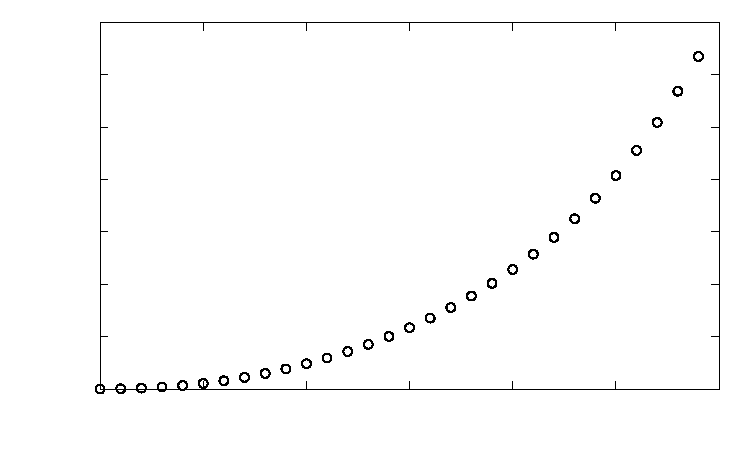
\includegraphics{GRAPH_SFR_Density}}%
    \gplfronttext
  \end{picture}%
\endgroup

					}\endgroup
			\caption{Graph of star formation rate density with redshift.\label{fig:GRAPH_SFR_Density}}
		\end{figure}
	% subsection critical_star_formation_rate_density (end)

	\subsection{Star Formation Rate Density} % (fold)
	\label{sub:star_formation_rate_density}
		The star formation rate density was approximated from the luminosity density, as per Equation~(\ref{eq:sfr_estimate})\cite{interactions_and_Induced_Star_Formation}
		\begin{align}
			\rho_\text{SFR}(M_\odot yr^{-1} Mpc^{-3})=1\times 10^{-28} \rho_L \label{eq:sfr_estimate}
		\end{align}
		where $\rho_L$ is spectral luminosity density in the region of $2150\pm 650 \AA$ in units of \si{\erg\per\second\per\hertz\per\cubic\mega\parsec}. Within this region it was assumed that the spectral luminosity density is constant. It was calculated from the integral of the Schechter function, multiplied by the luminosity, in terms of spectral luminosities. Since the characteristic magnitude parameters of the Schechter function were obtained in terms of AB Magnitudes, a conversion between AB Magnitudes and Spectral Luminosities was used.
		\begin{align}
			F_v = 10^{0.4(5-AB-48.6)}
		\end{align}
		Where $F_v$ is the Spectral Flux Density in units of \si{\erg\per\second\per\hertz\per\square\centi\metre} and AB is a monochromatic AB Magnitude see Appendix~\ref{sec:magnitude_to_spectral_luminosity}. This was used in conjunction with
		\begin{align}
			L_v=4\pi D_L^2 F_v
		\end{align}
		Where $L_v$ is a Spectral Luminosity in units of \si{\erg\per\second}, and $D_L$ if the luminosity distance of 10\,parsecs.	The lower luminosity limit on the Schechter function in Figure~\ref{fig:GRAPH_SFR_Density} corresponds to the spectral luminosity of galaxies with the smallest mass possible, discussed in Section~\ref{ssub:minimum_galaxy_mass}.

		\subsubsection{Minimum Galaxy Mass} % (fold)
		\label{ssub:minimum_galaxy_mass}
			In order to find the minimum mass, the redshift at which the Jeans mass (equation~\ref{eq:jeanssmass}) and the characteristic mass of a dark matter halo, (equation~(\ref{eq:characteristic_dark_halo}), were equal, was considered\cite{Barkana2001125}
			\begin{align}
				M^*=10^{13}h^{-1}(1+z)^{-4} M_\odot \label{eq:characteristic_dark_halo}
			\end{align}
			The Jeans Mass defines the critical mass of a cloud at which it will collapse to form a galaxy, thereby limiting the minimum mass of a star forming galaxy.\cite{Barkana2001125}.
			\begin{align}
				M_J \approx 5.73\times10^3 \left (\frac{1+z}{10} \right )^{3/2} M_{\odot} \label{eq:jeanssmass}
			\end{align}
			At the redshift at which these equations are equal, the mass of the galaxy was assumed to be separate and distinct from the rest of the mass of the universe. This assumption ensured that no additional matter could contribute to the mass of the gas after this point. The redshift at which this occurs was calculated to be z=106. This corresponds to a minimum mass of a galaxy of $M=1.1\times10^5M_\odot$.

			Adopting a Mass-Luminosity ratio of 1:1 for simplicity, the minimum mass was found to correspond to an upper limit on the luminosity of the galaxy of $1.1\times 10^5 L_\odot$. However this was a bolometric luminosity, representing power over all frequencies, as opposed to a spectral luminosity, the power at  a specific frequency. Thus, a conversion between bolometric luminosity and spectral luminosity was formulated.
		% subsubsection minimum_galaxy_mass (end)
	% subsection star_formation_rate_density (end)

		\subsection{Bolometric Luminosity to Spectral Luminosity} % (fold)
		\label{sub:bolometric_luminosity_to_spectral_luminosity}
			In order to deduce a relation between bolometric luminosity and spectral luminosity, it was necessary to approximate the shape of the spectrum of a typical galaxy. A blackbody spectrum of temperature $1\times 10^5$K. was used to represent this spectrum, as this temperature corresponds to the temperature of a source emitting at \SI{2150}{\angstrom} using
			\begin{align}
				\frac{3}{2}kT=hv
			\end{align}
			where $k$ is the Boltzmann Constant, $T$ is the temperature (K), $h$ is the Planck's constant and $v$ is frequency (Hz). As spectral luminosity is luminosity per unit frequency, it can be written that
			\begin{align}
				\int^{\infty}_{-\infty}L_v \d{v} = \int^{\infty}_{0}L_v \d{v} = L_\text{Bol}
			\end{align}
			where $L_\text{Bol}$ is the bolometric luminosity, in units of \si{\erg\per\second}. The intensity of a blackbody is proportional to the spectral luminosity, at a constant solid angle and surface area, therefore it follows
			\begin{align}
				L_v &= kI(v,T) \\
				\int^{\infty}_{0}L_v \d{v} &= L_\text{bol} \\
				k\int^{\infty}_{0}I \d{v} &= L_\text{bol} \\
				L_v &= \frac{I(v,T)}{\int^{\infty}_{0}I \d{v}} \times L_{bol}
			\end{align}
			% where$k$ is a constant, and $I(v,T)$ is the intensity as a function of frequency and temperature. $L_\text{Bol}/k$ was computed to be \SI{75224.6}{\erg\per\second\per\omega\per\square\centi\metre}.
			\begin{align}
				I(v,T)=\frac{8\pi v^2}{c^3}\frac{hv}{e^\frac{hv}{kT}-1}
			\end{align}
			where, within $I(v,T)$, $v$ is the frequency in Hertz corresponding to $2150\pm 650$ \AA, and $T=1.1\times 10^5$K. The lower limit of spectral luminosity in the UV range, corresponding to 2150\AA, therefore, was calculated to be $L_v =9.755\times 10^{21}$\,\si{\erg\per\second\per\hertz}.
		% subsection bolometric_luminosity_to_spectral_luminosity (end)

		\subsection{Upper Redshift Limit of Reionization} % (fold)
		\label{sub:upper_redshift_limit_of_reionization}
			In order to compute the luminosity density, it was necessary to convert the Schechter function integral into a gamma function. See Appendix~\ref{sec:schechter_function_to_gamma_function}. This permitted the actual star formation rate density to be computed. Subsequently both star formation rate density and critical star formation rate density were plotted against redshift in Figure~\ref{fig:GRAPH_SFR_CriticalSFR}.
			\begin{figure}[htbp]
				\centering
					\begingroup\endlinechar=-1
						\resizebox{0.8\textwidth}{!}{%
							% GNUPLOT: LaTeX picture with Postscript
\begingroup
  \makeatletter
  \providecommand\color[2][]{%
    \GenericError{(gnuplot) \space\space\space\@spaces}{%
      Package color not loaded in conjunction with
      terminal option `colourtext'%
    }{See the gnuplot documentation for explanation.%
    }{Either use 'blacktext' in gnuplot or load the package
      color.sty in LaTeX.}%
    \renewcommand\color[2][]{}%
  }%
  \providecommand\includegraphics[2][]{%
    \GenericError{(gnuplot) \space\space\space\@spaces}{%
      Package graphicx or graphics not loaded%
    }{See the gnuplot documentation for explanation.%
    }{The gnuplot epslatex terminal needs graphicx.sty or graphics.sty.}%
    \renewcommand\includegraphics[2][]{}%
  }%
  \providecommand\rotatebox[2]{#2}%
  \@ifundefined{ifGPcolor}{%
    \newif\ifGPcolor
    \GPcolortrue
  }{}%
  \@ifundefined{ifGPblacktext}{%
    \newif\ifGPblacktext
    \GPblacktexttrue
  }{}%
  % define a \g@addto@macro without @ in the name:
  \let\gplgaddtomacro\g@addto@macro
  % define empty templates for all commands taking text:
  \gdef\gplbacktext{}%
  \gdef\gplfronttext{}%
  \makeatother
  \ifGPblacktext
    % no textcolor at all
    \def\colorrgb#1{}%
    \def\colorgray#1{}%
  \else
    % gray or color?
    \ifGPcolor
      \def\colorrgb#1{\color[rgb]{#1}}%
      \def\colorgray#1{\color[gray]{#1}}%
      \expandafter\def\csname LTw\endcsname{\color{white}}%
      \expandafter\def\csname LTb\endcsname{\color{black}}%
      \expandafter\def\csname LTa\endcsname{\color{black}}%
      \expandafter\def\csname LT0\endcsname{\color[rgb]{1,0,0}}%
      \expandafter\def\csname LT1\endcsname{\color[rgb]{0,1,0}}%
      \expandafter\def\csname LT2\endcsname{\color[rgb]{0,0,1}}%
      \expandafter\def\csname LT3\endcsname{\color[rgb]{1,0,1}}%
      \expandafter\def\csname LT4\endcsname{\color[rgb]{0,1,1}}%
      \expandafter\def\csname LT5\endcsname{\color[rgb]{1,1,0}}%
      \expandafter\def\csname LT6\endcsname{\color[rgb]{0,0,0}}%
      \expandafter\def\csname LT7\endcsname{\color[rgb]{1,0.3,0}}%
      \expandafter\def\csname LT8\endcsname{\color[rgb]{0.5,0.5,0.5}}%
    \else
      % gray
      \def\colorrgb#1{\color{black}}%
      \def\colorgray#1{\color[gray]{#1}}%
      \expandafter\def\csname LTw\endcsname{\color{white}}%
      \expandafter\def\csname LTb\endcsname{\color{black}}%
      \expandafter\def\csname LTa\endcsname{\color{black}}%
      \expandafter\def\csname LT0\endcsname{\color{black}}%
      \expandafter\def\csname LT1\endcsname{\color{black}}%
      \expandafter\def\csname LT2\endcsname{\color{black}}%
      \expandafter\def\csname LT3\endcsname{\color{black}}%
      \expandafter\def\csname LT4\endcsname{\color{black}}%
      \expandafter\def\csname LT5\endcsname{\color{black}}%
      \expandafter\def\csname LT6\endcsname{\color{black}}%
      \expandafter\def\csname LT7\endcsname{\color{black}}%
      \expandafter\def\csname LT8\endcsname{\color{black}}%
    \fi
  \fi
  \setlength{\unitlength}{0.0500bp}%
  \begin{picture}(7200.00,4320.00)%
    \gplgaddtomacro\gplbacktext{%
      \put(849,595){\makebox(0,0)[r]{\strut{} 0}}%
      \put(849,1098){\makebox(0,0)[r]{\strut{} 0.05}}%
      \put(849,1601){\makebox(0,0)[r]{\strut{} 0.1}}%
      \put(849,2104){\makebox(0,0)[r]{\strut{} 0.15}}%
      \put(849,2606){\makebox(0,0)[r]{\strut{} 0.2}}%
      \put(849,3109){\makebox(0,0)[r]{\strut{} 0.25}}%
      \put(849,3612){\makebox(0,0)[r]{\strut{} 0.3}}%
      \put(849,4115){\makebox(0,0)[r]{\strut{} 0.35}}%
      \put(951,409){\makebox(0,0){\strut{} 10}}%
      \put(1545,409){\makebox(0,0){\strut{} 11}}%
      \put(2139,409){\makebox(0,0){\strut{} 12}}%
      \put(2734,409){\makebox(0,0){\strut{} 13}}%
      \put(3328,409){\makebox(0,0){\strut{} 14}}%
      \put(3922,409){\makebox(0,0){\strut{} 15}}%
      \put(4516,409){\makebox(0,0){\strut{} 16}}%
      \put(5110,409){\makebox(0,0){\strut{} 17}}%
      \put(5705,409){\makebox(0,0){\strut{} 18}}%
      \put(6299,409){\makebox(0,0){\strut{} 19}}%
      \put(6893,409){\makebox(0,0){\strut{} 20}}%
      \csname LTb\endcsname%
      \put(144,2355){\rotatebox{-270}{\makebox(0,0){\strut{}Star Formation Raet Density ($\M_\odot$\si{\per\year\per\cubic\mega\parsec})}}}%
      \csname LTb\endcsname%
      \put(3922,130){\makebox(0,0){\strut{}Redshift ($z$)}}%
      \put(3922,4022){\makebox(0,0){\strut{}}}%
    }%
    \gplgaddtomacro\gplfronttext{%
      \csname LTb\endcsname%
      \put(5910,3821){\makebox(0,0)[r]{\strut{}Critical SFR Density}}%
      \csname LTb\endcsname%
      \put(5910,3635){\makebox(0,0)[r]{\strut{}SFR Density}}%
    }%
    \gplbacktext
    \put(0,0){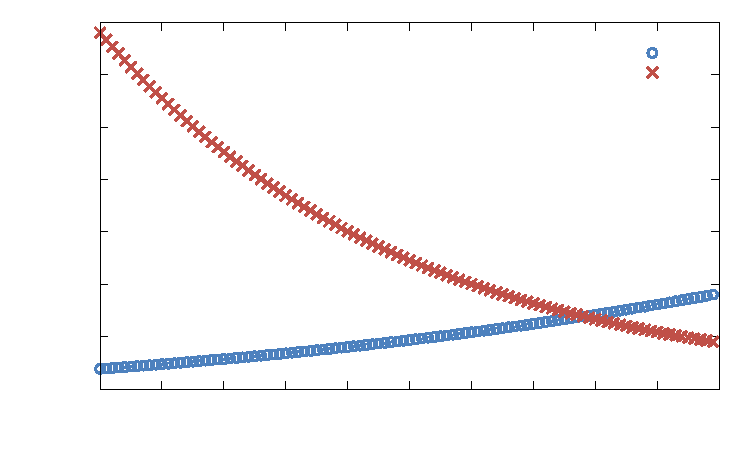
\includegraphics{GRAPH_SFR_CriticalSFR}}%
    \gplfronttext
  \end{picture}%
\endgroup

						}\endgroup
				\caption{Graph of star formation rate density and critical star formation rate.\label{fig:GRAPH_SFR_CriticalSFR}}
			\end{figure}

			As mentioned above the redshift at which the star formation rate density exceeds the critical star formation rate density will mark the beginning of reionization. This redshift corresponds to the point in Figure~\ref{GRAPH_SFR_CriticalSFR}, where the two curves intersect. The resultant redshift was found to be $z=17.82$.
		% subsection upper_redshift_limit_of_reionization (end)
% section calculating_the_timescale_of_reionization (end)

    % \section{Rate of Reionizing photons} % (fold)
\label{sec:rate_of_reionizing_photons}
	With a knowledge of the luminosity density, it is possible to calculate the star formation rate density, using the following formula.
	\begin{align}
		\rho_{SFR} &= 1\times 10^{-28}\rho_L
	\end{align}
	Using estimates of the fractional escape and zeta, we can use the formula above (7.7) to calculate the rate of reionization. From this, and the number of neutral hydrogen particles in the universe, it is possible to calculate the timescale of reionization.
	\begin{align}
	t =\frac{dNion}\d{t}\times \frac{1}{N_H}
	\end{align}
	Where t is the time between the start of reionization and the end, in seconds, Nion is the number of ionizing photons produced and $N_H$ is the number of Hydrogen atoms in the universe.

	As the number of photons produced roughly equalls the number of neutral hydrogen in the universe, it is possible to calculate a limit on the redshift accosiated with the end of reionization, given the corresponding opposite limit.

	A simulation of this was undergone using the equation above, and the resultant timescale was found to be\ldots

	\subsection{Techniques for Finding an Upper Limit on Redshift} % (fold)
	\label{sub:techniques_for_finding_an_upper_limit_on_redshift}
		We know that when $\rho_{SFR}$ and $\rho_{SFR}*$ are equal, reionization will begin. Knowing the Clumping factor (See Section X) it is possible to calculate the critical Star formation rate density, using the following equation,
		\begin{align}
		\rho_{SFR}*=2\times 10^3\frac{C}{f_{esc}} {\left( \frac{1+z}{10} \right )}^3
		\end{align}
		Where $f_{esc}$ is the fractional escape of photons from reionizing spheres, and C is the clumping factor. Combining with equation X it is possible to calculate the conditions for which reionization began as follows:
		\begin{align}
		1\times10^{-28}\int^{\infty}_{L}L\phi(L) dL=2\times 10^3\frac{C}{f_{esc}}{\left( \frac{1+z}{10} \right)}^3
		\end{align}
		Solving this equation, will give an upper z limit to reionization, and usign the timescale IN THE PREVIOUS SECTION it is possible to calculate both limits.

		The resultant values for redshift were z+/-z
	% subsection techniques_for_finding_an_upper_limit_on_redshift (end)

	\subsection{Jeans Mass for Collapse and Galaxy Formation} % (fold)
	\label{sub:jeans_mass_for_collapse_and_galaxy_formation}
		The Jeans Mass defines the cirtical mass of a cloud before it can collapse to form a galaxy, thereby limiting the minimum mass of a star foming galaxy. It is defined as the equation below:
		%\begin{align}
		%M_J=\left ( \frac{5kT}{Gm}\right ) ^{3/2} \left ( \frac{3}{4\pi\rho} \right ) ^{1/2}
		%\end{align}
		\begin{align}
		M_J = 5.73\times 10^3{\left(\frac{\Omega_mh}{0.15} \right)}^{-1/2} {\left( \frac{\Omega_b h^2}{0.022}\right)}^{-3/5} {\left( \frac {1+z}{10} \right)}^{3/2} M_\odot
		\end{align}
		Assuming an appropriate Mass-Luminosity ratio, this corresponds to an upper limit on both the Luminosity and the Absolute Magnitude (i.e.\ the dimmest ionizing galaxy.) This therefore provides a lower limit of magnitude to the schechter function, the L specified in the equation in the previous section

		\subsection{Mass-Luminosity Ratios}

		An appropriate Mass-Luminosity Formula is:
		\begin{align}
		L(M) = L_0 \times \frac {{(M/M_s)}^a} {q+{(M/M_s)}^{cd}}^{1/d}
		\end{align}
		where d=0.23, a=40 q=0.57 c=3.57\\
		\newline
		Or you can get the star formation rate of a galaxy from the mass (0911.1356v4) and from this you can obtain the Magnitude Kennicutt 1998 conversion from UV luminosity to AB magnitude and thereby to luminosity.
	% subsection jeans_mass_for_collapse_and_galaxy_formation (end)

	\subsection{Press Schechter Formalism} % (fold)
	\label{sub:press_schechter_formalism}
		PSF is a method of obtaining the number of objects with a specific mass within a certain volume. It assumes that the universe linearly ``clumped'' at the beginning of the universe, until a point where the density of the clumps break away from the rest of the universal expansion, and is treated as a massive body which collapses rapidly. (this occurs at around $\delta_c$\~1.68- Gunn and Gott). Press and Schechter suggest a probability distribution function of =:
		\begin{align}
		p(M,z)=-2p_0 \frac{\Delta P [\delta_v>\delta_c(z)]} {\Delta M} dM
		\end{align}
		Where $p_0$ is the mean density of the universe, and $\delta_c(z)$ is the overdensity threshold per redshift. P is the cumulative probability distribution of $\delta_v$ (volume)

		 It is from this that Schechter functions of luminosity and magnitude could arise\ldots
	% subsection press_schechter_formalism (end)

% section rate_of_reionizing_photons (end)

    %!TEX root = mainfile.tex

\section{Cosmic Variance} % (fold)
\label{sec:cosmic_variance}
	In general, the Universe can only be considered to be homogeneous at the most extreme distance scales ($>\SI{1}{\giga\parsec}$). At the scales which tend to be observed, matter in the Universe is not distributed uniformly and will gather together in massive clusters. Conversely, there will be empty regions of space, known as voids, where virtually no matter is present at all.

	Measurements deduced from observational surveys will certainly be affected by this large-scale cosmic structure. A measurement of an arbitrary region of the sky will have an associated uncertainty far greater than any sample variance due to Poisson statistics. This uncertainty is known as \emph{Cosmic Variance}, and will nearly always be the dominant source of error for any high-redshift cosmic survey. Given a probability distribution for the number counts, the cosmic variance is defined as:
	\begin{align}
		\sigma_v^2= \frac{\left \langle N^2 \right \rangle - \left \langle N \right \rangle^2}{\left \langle N \right \rangle}-\frac{1}{\left \langle N \right \rangle} \label{eq:cvstat}
	\end{align}
	where $\left \langle N \right \rangle$ is the mean and $\left \langle N^2 \right \rangle$ is the variance\cite{Trenti2008}.

	Any number or density measurement derived from a galaxy population is susceptible to cosmic variance. As an extreme example, it is reported to be potentially at the 50--70\% level in the HST UDF surveys\cite{Driver01102010}. Evidently, it will be particularly relevant to this study of cosmic re-ionization.

	\subsection{Factors which affect the Cosmic Variance} % (fold)
	\label{sub:factors_which_affect_the_cosmic_variance}
		Fortunately, there exist numerous ways of reducing the cosmic variance of a galaxy survey to a manageable amount, mostly accepted to be $<10\%$. As a general rule, this is achieved when a volume of \SI{e7}{\mega\parsec\cubed} is surveyed, with a square survey area over a single contiguous region\cite{Driver01102010}.

		The cosmic variance of a survey depends on three factors principally:
		\begin{itemize}
			\item it decreases steadily with volume
			\item it is reduced for higher aspect ratio surveys
			\item it is also reduced when multiple sight-lines are taken i.e.\ sparse sampling
		\end{itemize}
		Taking advantage of these factors, one can take steps to address the issue of cosmic variance.
	% subsection factors_which_affect_the_cosmic_variance (end)

		\subsubsection{Survey Volume} % (fold)
		\label{ssub:survey_volume}
			As mentioned above, the cosmic variance is heavily dependent on the volume of the survey, indicated by the steady decrease to lower percentages as larger volumes are surveyed, as in figure~\ref{fig:cv1}.  For volumes of \SI{e4}{\mega\parsec\cubed}, it is as much as 60\% whereas for \SI{e7}{\mega\parsec\cubed}, it will be 10\% and below.

			The dashed line below the main trend on the graph shows how the percentage uncertainty varies solely due to the sample variance. This gives some idea of the gulf between the effect of cosmic variance and that of Poisson statistics.
			\begin{figure}
				\centering
				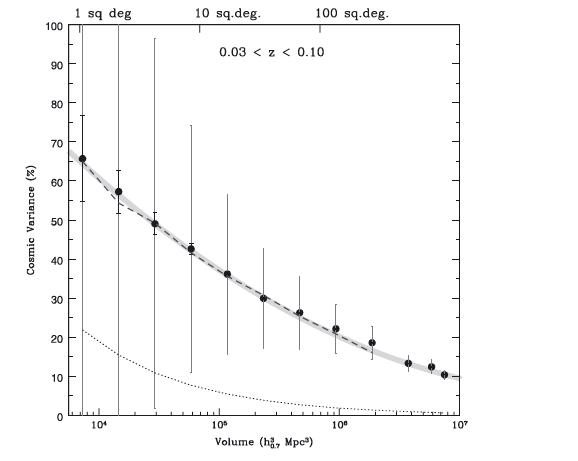
\includegraphics[width=0.7\textwidth]{../Images/cosmic_variance1.JPG}
				\caption{Graph showing the relation between the percentage cosmic variance and survey volume.\label{fig:cv1}}
			\end{figure}

			\begin{figure}
				\centering
				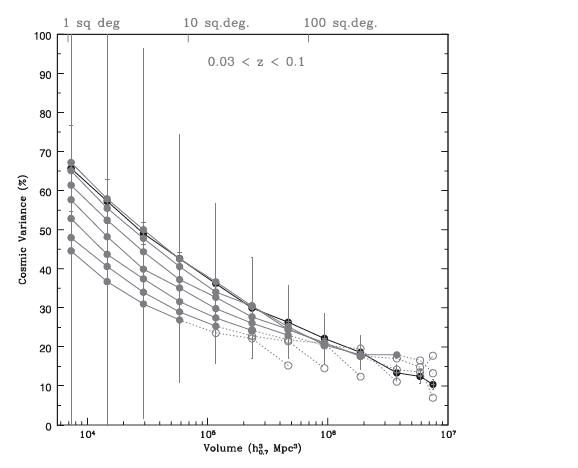
\includegraphics[width=0.7\textwidth]{../Images/cosmic_variance2.JPG}
				\caption{The same as for graph 1, this time with the additional grey points showing the dependence on aspect ratio. From the top to bottom they are 1:2, 1:4, 1:8, 1:16, 1:32, 1:64 and 1:128.}\label{fig:cv2}
			\end{figure}
		% subsubsection survey_volume (end)

		\subsubsection{Aspect Ratio} % (fold)
		\label{ssub:aspect_ratio}
			The aspect ratio of the survey is another crucial factor that can help deal with cosmic variance. For the same survey area, a long thin strip chosen over a standard square-shaped survey will decrease the cosmic variance. When taken to the extreme, this can cause a significant reduction. The same trend as for figure~\ref{fig:cv1} is shown in figure~\ref{fig:cv2}, but with the grey dots corresponding to higher aspect ratio surveys. The graph illustrates that, particularly for larger volumes, increasing the aspect ratio of a survey can make a huge reduction in the cosmic variance uncertainty.
		% subsubsection aspect_ratio (end)

		\subsubsection{Sparse Sampling} % (fold)
		\label{ssub:sparse_sampling}
			One might tackle cosmic variance in a very effective manner via the method of \emph{sparse sampling}, whereby several identical observing areas are distributed randomly across the sky. As opposed to one contiguous survey, these multiple sight-lines in different directions allow a more representative portion of the sky to be surveyed.

			It has been shown that cosmic variance is reduced with the number, $N$ of such sight-lines by $\frac{1}{\sqrt{N}}$. This holds irrespective of the base survey area\cite{Driver01102010}.
		% subsubsection sparse_sampling (end)

	\subsection{General Formula} % (fold)
	\label{sub:general_formula}
		In order to address cosmic variance in the code itself, an empirical formula was employed. In a paper (Driver and Robotham, 2010), this formula was derived using data from the SDSS (Sloan Digital Sky Survey), and extrapolated out to higher redshifts\cite{Driver01102010}. Due to its extrapolated nature, it should be noted that this is an approximate formula. Nonetheless, it should output a robust estimate of the cosmic variance for given surveys. Additionally, through it one can deduce possible ways to reduce the cosmic variance to below 10\%.
		\begin{align}
			\zeta _{CV}(\%)=\frac{\left( 1.00-0.03\sqrt{X-1} \right)\times \left( 219.7-52.4\log_{10}\left(291.0\times AB \right) + 3.21\log_{10}{\left(291.0\times AB\right)}^{2} \right)}{\sqrt{NC/291.0}} \label{eq:cvmain}
		\end{align}
		The formula employs the median redshift transverse lengths $A$ and $B$, and the radial depth $C$, all given in \si{\mega\parsec}, to represent the volume of each survey sample. The number of such samples i.e.\ the number of sight-lines is $N$. The aspect ratio is dealt with in the amplitude term at the front of the expression, where the aspect ratio 1:128 would be submitted as $X=128$, for example.

		Although it is extrapolated from an equation that applies at $z<0.1$, it takes advantage of the fact that cosmic variance should vary according to Poisson statistics along the radial length. This means that a survey with twice the radial depth will have $\sqrt{2}$ less cosmic variance. Hence the factor of $\sqrt{C}$ in the denominator. Equation~\ref{eq:cvmain} does not, however, make any corrections for the evolution of the clustering signature of the galaxy population, with this expected to be lower towards higher redshift. Correspondingly, any estimate output should be treated as an upper limit.

		This equation has been entered into the code which, from the survey parameters input, calculates the required quantities and gives an estimate of the cosmic variance as a percentage of the number counts expected to be observed. Furthermore, it will inform the user of how many random pointings of such a survey are necessary to achieve less than $10\%$ cosmic variance.
	% subsection general_formula (end)
% section cosmic_variance (end)

%written and researched by Lewis Clegg, coded by Andy King.

    %!TEX root = mainfile.tex

\section{Gravitational Lensing Bias} % (fold)
\label{sec:gravitational_lensing_bias}
	It is well known that the effect of gravitational lensing is a powerful tool, which can manageably be exploited to boost the magnification of intrinsically faint or very distant galaxies (see Section- grav lensing). However, it is now thought that the high incidence of gravitational lensing in high-redshift observations will distort flux and number density measurements of the earliest galaxies\cite{distortionsinthegravitationallens}. A recent study (Wyithe and Stuart 2011) makes the case that the Hubble Space Telescope's (HST) current view of these galaxies has been significantly altered by gravitational lensing. Moreover, any planned galaxy surveys in the future, such as those with the James Webb Space Telescope (JWST), need to be designed to account for these substantial lensing biases at these extreme distances\cite{wyithestuart2011}.

	\subsection{Magnification Bias} % (fold)
	\label{sub:magnification_bias}
		Along a random line of sight, the light from distant source objects may be distorted- appearing brighter or being fragmented, so it is observed as multiple images- due to gravitational lensing by galaxies in the foreground. The raw probability of multiple imaging for high-redshift objects is ~0.5\%. However, the statistics can potentially become skewed by far greater amounts owing to something known as \emph{magnification bias}. Essentially, this is the magnification of intrinsically faint galaxies- that otherwise would be undetectable- to observed fluxes above the limit for a particular survey, leading to an excess of lensed galaxies among flux-limited samples. This magnification bias is expected to be significant at $z>8$. This would mean, for example, that if in an observation at $z>10$ there existed only a few galaxies above the detection limits, this number could be boosted by an order of magnitude, so that 10--30 galaxies were actually observed\cite{Cosmicmagnifyinglenses}. Consequently, gravitational lensing will likely dominate the observed properties of such early galaxies.

		The study, mentioned above, assesses the magnification bias among high-redshift galaxies in the Hubble Ultra-Deep Field (HUDF) by calculating the fraction of galaxies above the magnitude limit which will have been multiply imaged. They predict that at $z\approx6-7$, around 1\% of galaxies will be lensed; at $z\approx8-10$ this fraction can increase to up to a few tens of percent\cite{wyithestuart2011}. It should be noted that these values are subject to increasing sensitivity, at higher redshifts, to the true value of the characteristic magnitude M* (see section-Schechter function?)- as the survey limit may get much closer to M*, whose value is still highly uncertain. This sensitivity is illustrated in~Figure \ref{fig:gravhst1}, with the fraction of multiply lensed galaxies, $F_{mult}$, expected to be seen at different redshifts. One can clearly see that gravitational lensing biases become more of an issue the higher the redshift being observed.

		The corresponding graph in Figure~\ref{fig:gravjwst1} gives some idea of how this factor will continue to be an issue as telescopes with increased optical depth and resolution, such as JWST, become operational. For the ultra-deep and medium deep surveys, a multiply imaged fraction higher than $F_{mult}\approx10\%$ could be observed at $z>12$ and $z>16$ respectively.

		The magnification bias will additionally cause an overconcentration of high-redshift galaxies around foreground clusters. This correlation could be considered as an alternative means of studying the effects of gravitational lensing. For the JWST, it is thought that the majority of galaxies at extreme redshifts ($z>14$) will be $<1~arcsec$ from a bright foreground galaxy, meaning they will have been gravitationally magnified into the sample- a startling prediction\cite{wyithestuart2011}.
		\begin{figure}
			\centering
			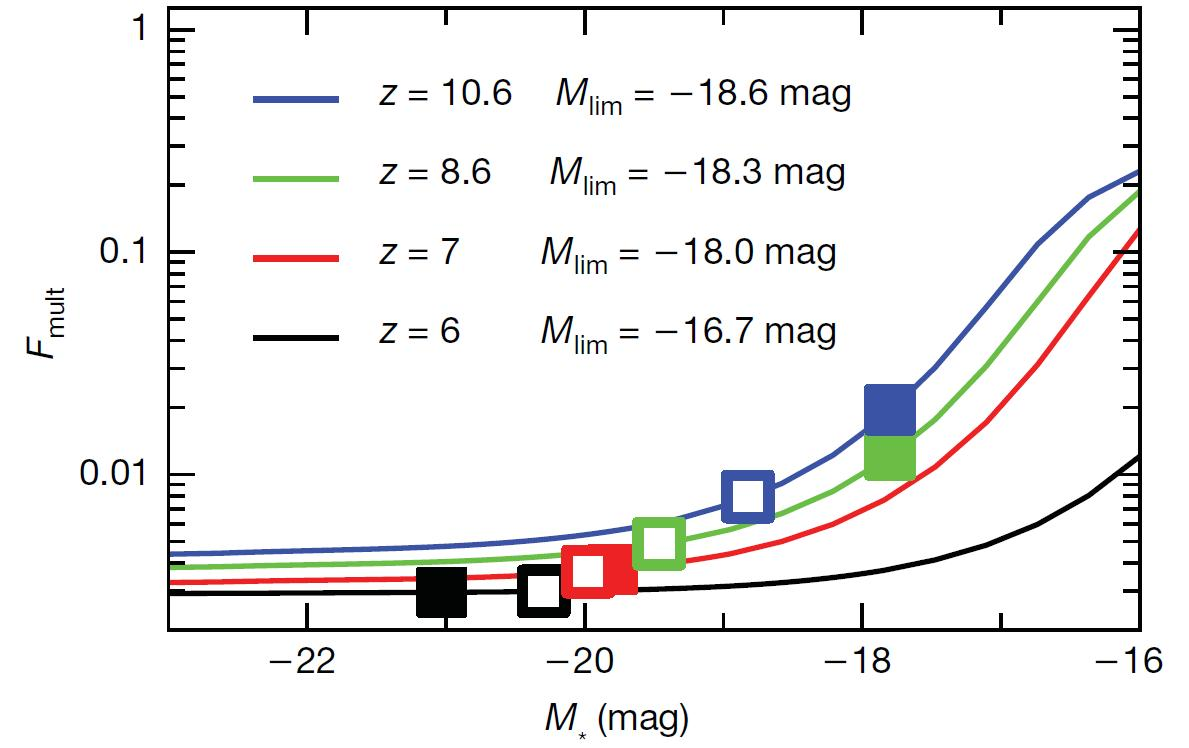
\includegraphics[width=0.6\textwidth]{../Images/gravhst1.JPG}
			\caption{Graph showing the fraction of galaxies that are multiply imaged,  $F_{mult}$, at different redshifts, as a function of the characteristic magnitude, M*, for the HST. The closed and open squares represent alternative estimates of M*.}\label{fig:gravhst1}
		\end{figure}

		\begin{figure}
			\centering
			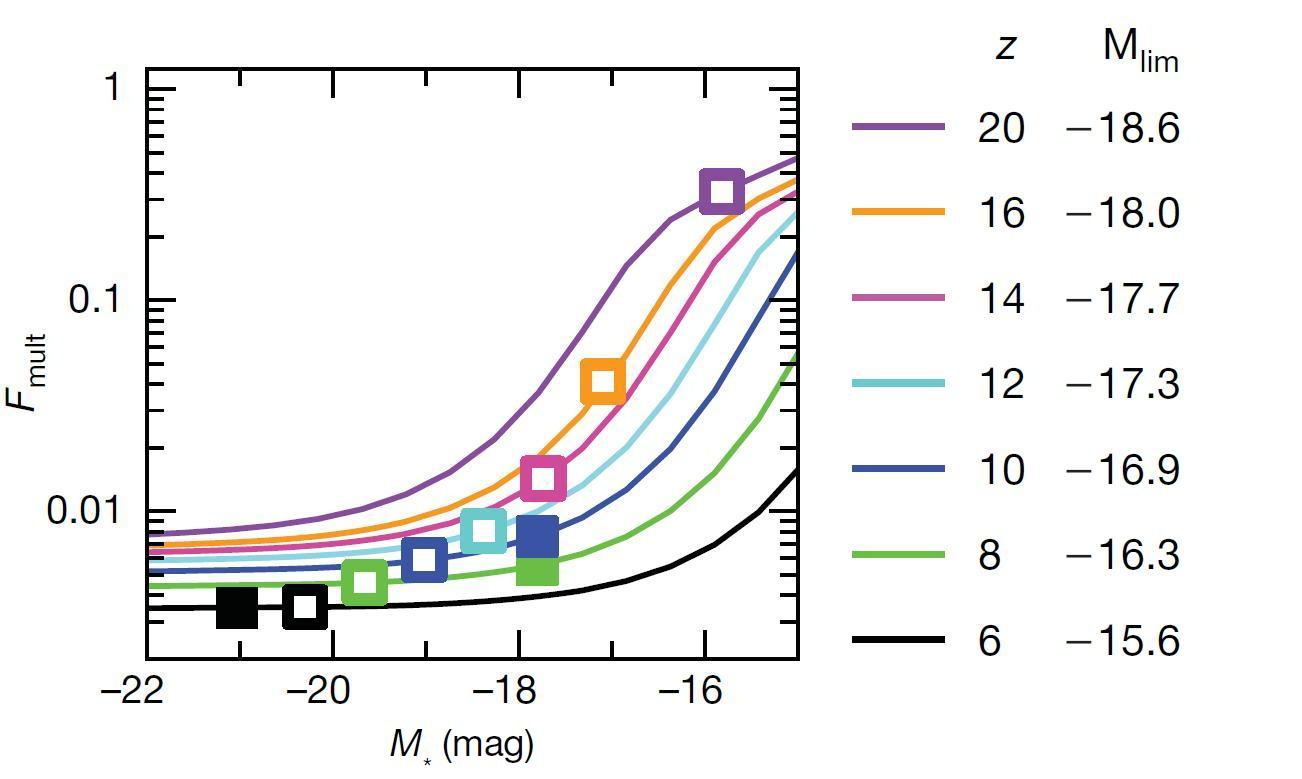
\includegraphics[width=0.6\textwidth]{../Images/gravjwst1.JPG}
			\caption{Graph showing the fraction of multiply imaged galaxies against M* at different redshifts, for the JWST ultra-deep survey.}\label{fig:gravjwst1}
		\end{figure}
	% subsection magnification_bias (end)

	\subsection{Effect on the Luminosity Function} % (fold)
	\label{sub:effect_on_the_luminosity_function}
		The distortion of galaxy number counts and their observed magnitudes brought about by the magnification bias will have a profound effect on the luminosity function, the properties of which, currently beyond $z\approx8$, are highly uncertain.~Figure \ref{fig:gravlumfun} illustrates the potential for the dramatic effect gravational lensing can have on the shape of the luminosity function.

		Current luminosity functions at $z>7$ are not corrected in any way for gravitational lensing. Any future studies will need to be prescribed with a detailed understanding of the magnification bias of high-redshift sources in order to discover the veritable unlensed shape of the luminosity function. However, allowing for the precise modelling of the involved biases, the exploitation of the correlation of high-z sources and foreground galaxies will be invaluable for probing the otherwise inaccessible shape of the luminosity function at these redshifts.
		\begin{figure}
			\centering
			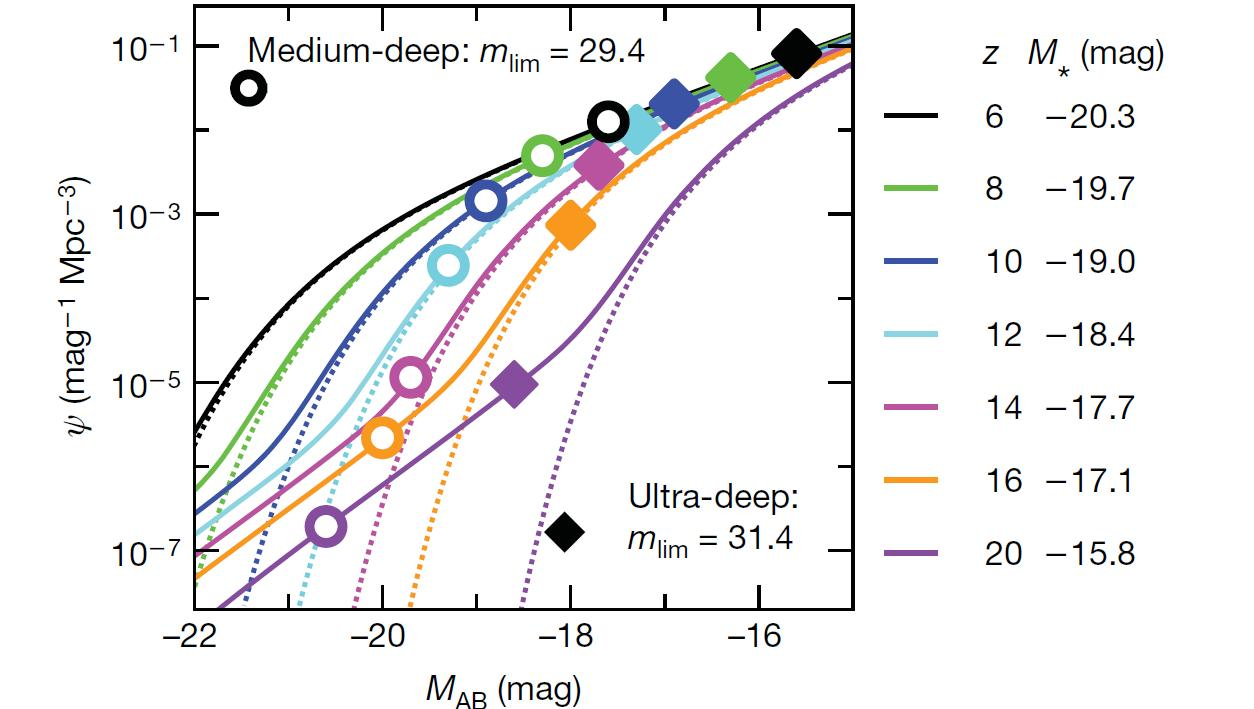
\includegraphics[width=0.6\textwidth]{../Images/gravlumfun.JPG}
			\caption{Graph detailing the lens-induced distortion of the luminosity function. Dashed lines represent the unlensed shape, solid lines the modified shape due to gravitational lensing.}\label{fig:gravlumfun}
		\end{figure}
	% subsection effect_on_the_luminosity_function (end)

% section gravitational_lensing_bias (end)





    %!TEX root = mainfile.tex

\section{Clumping Factor} % (fold)
\label{sec:clumping_factor}
(Lewis)

	hydrogen which already has been reionized may still play a significant role in the evolution of the Universe during the epoch of reionization, as it is still possible for it to recombine and become neutral once more. The average rate of recombinations is a significant factor which acts to slow down the expansion of the ionization front into the neutral inter-galactic medium. This rate, in turn, is proportional to a value known as the Clumping Factor. This factor is essentially a measure of the inhomogeneity in a medium, in this case, ionized hydrogen. In the what is known as the density field method, it is simply given by
	\begin{align}
		C_{DF} &=\frac{\left \langle n_\text{HII}^2 \right \rangle}{\left \langle n_\text{HII} \right \rangle^2}, \label{eq:clumpingnHII}
	\end{align}
	where $n_\text{HII}$ is the number density of ionized hydrogen in the inter-galactic medium, and $\left \langle n_\text{HII} \right \rangle$ is the average of this value\cite{2012ApJ...747..100S}.

	Many analytical and computational models are available which use the clumping factor to correct for recombinations during the reionization process. Some treat it as a global parameter, that is constant at all points in space. However, many believe a single value of the clumping factor will overestimate the recombination rate. Consequently, they choose to adopt a local parameter, which varies due to the density gradient of the inter-galactic medium. This also accounts for the negligible contribution of neutral gas to the recombination\cite{MNL2:MNL2993}.

	Other simulations generate a clumping factor which evolves over the period during which reionization took place. One such model (Iliev et al.~2007) has clumping evolving with redshift as\cite{Pawlik21042009},
	\begin{align}
		C &=26.2917\times \e{-0.1822z+0.003505z^2}. \label{eq:clumpingredshift}
	\end{align}
	For simplicity, in this project, the simpler method using a global variable was chosen. However, a redshift dependence scenario corresponding to that from equation~(\ref{eq:clumpingredshift}) was adopted, for better accuracy in the evolution of the critical star formation rate.
% section clumping_factor (end)

    %!TEX root = mainfile.tex

\section{Galaxy Number Predictions} % (fold)
\label{sec:galaxy_number_predictions}
	One of the central tasks of the predictions subgroup is to make informed predictions regarding the distribution of galaxies around and during the epoch of reionization. As previously described, the distribution of galaxies in the early universe can be modelled using a Schechter function
	\begin{align}
		\Phi_L = \Phi^*  \left(\frac{L}{L^*}\right)^\alpha \exp{\left( -\frac{L}{L^*} \right)} \frac{1}{L^*}
	\end{align}
	Ultimately, it will be necessary to resort to numerical calculations to extract meaningful predictions from this model, but it is useful and instructive to begin with an analytical approach.

	\subsection{Analytical Approach} % (fold)
	\label{sub:analytical_approach}
		We use the Schechter function to decribe the number density of galaxies per unit luminosity; in order to extract a true number density from this we must integrate across the relevant range of luminosities
		\begin{align}
			n = \int_{L_1}^{L_2}\Phi_L \d{L}.
		\end{align}
		In general, the luminosity function (and, therefore, the number density) will vary as a function of position, $\Phi_L = \Phi_L (L,\underline{\mathbf{r}})$, so in order to extract the number of galaxies in some finite volume we must integrate across the volume
		\begin{align}
			N = \int_V n(\underline{\mathbf{r}}) \d{V} ,
		\end{align}
		resulting in the double integral
		\begin{align}
			N = \int_V \int_{L_1}^{L_2} \Phi_L(L,\underline{\mathbf{r}}) \d{L} \d{V} .
		\end{align}
		If the volume of space considered spans a sufficiently large area of sky then we can invoke the large scale isotropy implied by the cosmological principle to argue that, in effect, $\Phi_L$ is not dependent upon the full position vector, $\underline{\mathbf{r}}$, but only its radial component, $r$. Furthermore, since there is a one to one relationship between distance from earth, $r$, and cosmological redshift, $z$, $\Phi_L$ can be expressed as a function of just $L$ and $z$.
		\begin{align}
			\Phi_L &= \Phi_L(L,r); \qquad r= r(z);\\
			\therefore	\Phi_L &= \Phi_L(L,z).
		\end{align}
		The inaccuracy of this simplification on smaller scales is considered in more depth later, in the section on cosmic variance. The volume of integration can then be chosen to be a spherical shell with limits of constant redshift, so that the volume integration may be carried out over concentric and infinitesimal redshift shells
		\begin{align}
			N = \int_{z_1}^{z_2} \int_{L_1}^{L_2} \Phi_L(L,z) \d{L} \dx{V}{z} \d{z}.
		\end{align}
		From equation~(\ref{eq:comoving_distance}), we know that
		\begin{align}
			\dx{r}{z} &= \frac{c}{H(z)}.
		\end{align}
		Together with the form of the volume, we can use this to find the derivative $\dx{V}{z}$
		\begin{align}
			\dx{V}{z} &= \dx{V}{r} \cdot \dx{r}{z} \\
		 			&= \dx{}{r} \left[\frac{4}{3} \pi r^3 \right ] \cdot \frac{c}{H(z)}\\
					&= 4 \pi r^2 \cdot \frac{c}{H(z)} \\
					\Rightarrow	\dx{V}{z}	&= \frac{4 \pi r^2 c}{H(z)}
		\end{align}
		Applying this substitution results in
		\begin{align}
					N = \int_{z_1}^{z_2} \int_{L_1}^{L_2} \Phi_L(L,z) \frac{4 \pi r^2 c}{H(z)} \d{L}\d{z}
		\end{align}
		Where the value of r is also found using equation~(\ref{eq:comoving_distance})
		\begin{align}
			N = \int_{z_1}^{z_2} \int_{L_1}^{L_2} \Phi_L(L,z) \frac{4 \pi c}{H(z)}\d{L}\d{z} \left[ \int_0^{z}\frac{c }{H(z')} \d{z'} \right ]^2
		\end{align}
		In practice, luminosities are most commonly measured in terms of absolute magnitude, M, so in order to align with convention we use the magnitude equivalent of the luminosity function and substitute
		\begin{align}
			\int \Phi_L \d{L} = \int \Phi_M\d{M} ,
		\end{align}
		where
		\begin{align}
			\Phi_M = 0.4 \ln(10) \Phi^* 10^{0.4(M^*-M)(\alpha+1)} \exp(-10^{0.4(M^*-M)})
		\end{align}
		The full derivation of the magnitude Schechter function is given in appendix~\ref{app:derivation_of_magnitude_schechter_function}. Applying this substitution gives
		\begin{align}
			N = \int_{z_1}^{z_2} {\int_{M_1}^{M_2} { \Phi_M(M,z) \frac{4 \pi c}{H(z)} \d{M} \d{z} \left[ \int_0^{z}{\frac{c }{H(z')} \d{z'}}\right ]^2} } .
		\end{align}
		Finally, by substituting in the we substitute in the Schechter function
		\begin{align}
					N = \frac{4 \pi c^3}{H_0^3} \int_{z_1}^{z_2}  \frac{1}{E(z)} \left[ \int_0^{z}{\frac{1}{E(z')} \d{z'} }\right ]^2 \d{z} \int_{M_1}^{M_2} \Phi_M(M,z) \d{M}
		\end{align}
	% subsection analytical_approach (end)

	\subsection{Numerical Computation} % (fold)
	\label{sub:numerical_computation}
		The complexity of this analytical solution makes it an impractical approach for real calculations, so in most cases numbers of galaxies are computed numerically by splitting the M and z continuum into a two dimensional array of discrete redshift shells and magnitude bins. The resulting summation takes the form
		\begin{align}
			N = \sum_i \sum_j \Phi_M(z_i,M_j) \Delta V(z_i) \Delta M_j . \label{eq:galaxy_number_double_sum}
		\end{align}
		Where $\Delta V(z_i)$, is the volume of the thin, but finite spherical shell between redshift $z_i$ and $z_{i+1}$, and is calculated using the standard equation for the volume of a spherical shell
		\begin{align}
			\Delta V = \frac{4}{3} \pi ( d_{i+1}^3 - d_{i}^3)
		\end{align}
		The Schechter parameters used were designed for use with comoving volumes, so the distances used are comoving distances calculated from $z$ using the standard integral relationship given in equation~(\ref{eq:comoving_distance}), which is also solved numerically.

		equation~(\ref{eq:galaxy_number_double_sum}) can be seen as the direct but approximate equivalent of the double integral
		\begin{align}
			N = \int_V \int_{M_1}^{M_2} \Phi_M(z,M) \d{M} \d{V} ,
		\end{align}
		before it is taken to the continuum limit of infinitesimal $\Delta M$ and $\Delta V$, which makes the calculation mathematically exact.

		In order to carry out these calculations a program was built. The focus of the constructed program was not to calculate any specific result for the number of galaxies in some fixed magnitude and redshift range, but to provide an efficient and adaptable means to calculate the distribution of observable galaxies in any input ranges in the region of cosmic reionization.

		This flexibility allows for the efficient calculation of results tailored for any proposed survey, such that the survey's validity and usefulness can be assessed and determined. The results of these specific calculations and the observing strategies they suggest and inform are discussed in the latter part of this report.

		The variation in the form of the Schechter function was accounted for by including the calculated models for the evolution of the Schechter parameters with redshift in Section~\ref{sec:parameter_values}. The uncertainties in the evolution models were used to calculate upper and lower estimates for the galaxy number predictions, however, the lower estimates were universally zero because of the large uncertainties inherrent to the data currently available. The upper estimate did provide useful results which, in most cases, were approximately triple the value of the best estimate.
		% subsection numerical_computation (end)
% section galaxy_number_predictions (end)


    \section{Conclusion} % (fold)
\label{sec:conclusion}
	The predictions subgroup were responsible for providing original calculations dating the timescale of re-ionization and to provide a means by which the number of galaxies within a certain magnitude range and volume of sky could be calculated.

	The beginning of the EoR was determined by analytically calculating the star formation rate density using a lower limit of luminosity in the Schechter function, corresponding to the Jeans mass when the galaxy formed. Comparing this result to a model of critical star formation rate density a redshift at which reionization began was obtained, giving \emph{$z=17.82$}.

	The lower redshift bound was calculated similarly and evolved as more sophisticated physics was included. The first model assumed constant $\zeta$ and $f_\text{esc}$ and no recombinations giving a lower limit redshift of an ionized universe at \emph{$z=6.3\pm 1.7$}. This model gave the closest value when compared to literature despite it including many oversimplifying assumptions. The second model included an evolving escape fraction from compiled data from various sources. This gave a redshift of \emph{$z=7.5\pm 2.1$} with the greater errors due to the uncertainty of fesc. Finally the third model took into account both recombinations and an evolving escape fraction to give \emph{$z=7\pm 1.8$}. This value implies that cosmic reionization occurred earlier than the literature suggests however methodically it is more accurate as less simplifying assumptions were included.

	A further program was built in order to provide an efficient and adaptable means to calculate the distribution of observable galaxies in any input ranges in the region of cosmic reionization. It doesn’t to calculate any specific result for the number of galaxies in some specified magnitude and redshift range so as not to limit its capabilities. This flexibility has allowed an economical calculation of results that are easily tailored to any survey.

	The effect of cosmic variance was considered to be a significant factor for any observations to be made.
	Subsequently an empirical formula was located and implemented in the code to address cosmic variance giving it as an estimated percentage of the number of galaxies expected in the survey area.
% section conclusion (end)

% part predictions (end)
\newpage
\part{Observations} % (fold)
\label{prt:observations}
    %!TEX root = mainfile.tex
\section{Observing Strategy Group} % (fold)
\label{sec:observing_strategy_group}
	This primary aim of this subgroup is to formulate an observing strategy capable of probing the depths of the Epoch of Re-ionization. Our strategy is going to be based upon using optical techniques to detect candidate Lyman Break Galaxies (LBG) and confirming their properties using spectroscopy.

	The study of this era in the universe’s history has come a long way in the past 30 years and with the selection of new telescopes and radio arrays being designed currently it is only set to accelerate over the coming decades. It is a massive understatement to say such distant redshifts are very difficult to see and it is a testament to scientific and engineering achievement that we are able to take the detailed images we can. The light from these galaxies is so faint that it can take a very long time to see anything. Due to this lengthy nature of the projects, time on telescopes is highly sought after and very competitive.

	This strategy must therefore be as complete as possible with as many influencing factors included. This strategy will have two main focuses:
	\begin{itemize}
		\item Using the most efficient methods available in order to limit the observing time required.
		\item To probe the beginning of re-ionization; there have been few observations above $z=10$ and future telescopes will have the ability to break new frontiers and observe what happened at these earliest moments of structure formation.
	\end{itemize}

	Our strategy will look to utilise the capabilities of the new technology to further the scientific understanding of the EoR.

	The observing strategy will be established as follows:
	\begin{itemize}
		\item Research possible telescopes capable of observing high-redshift objects.
		\item Explore the advantages and disadvantages of ground and space-based telescopes.
		\item Identify the most efficient telescope for a wide survey of the sky to locate candidates; this will be determined using exposure time calculations.
		\item Research gravitational lensing, its possible application in assisting our wide surveys and how we might locate more lenses.
		\item Identify the telescope which will produce the highest resolution imaging of in a narrower deep survey; this will be established using exposure time calculations and observational limits of the system.
		\item Identify a telescope capable of spectroscopically confirming the nature and redshift of the candidates.
		\item Investigate the application of methods such as colour-colour diagrams for selecting candidates and removing contaminants from the sample.
		\item Compile a ‘Final Observing Strategy’ capable of observing the EoR using numerical predictions from the predictions subgroup.
	\end{itemize}
	This `Final Observing Strategy' will give calculations of the observation time required (inc.\ photometry, overheads, spectroscopy), the timescale on which the project can be actioned, the limitations of our strategy, possible areas for optimisation/refinement and areas for further research.

% section observing_strategy_group (end)

    %!TEX root = mainfile.tex

\section{Determining Redshift} % (fold)
\label{sub:determingin_redshift}
	Need a section on candidates and how the contaminants are eliminated.
	(COMBINE WITH JOE'S COLOUR STUFF?)

	Section~\ref{sec:contaminants} described how contaminants could be eliminated from the large number of potential high redshift galaxies. Taking the remaining objects, the following methods are used to check whether they are in fact LBGs.

	\subsection{Filters and the Dropout Technique} % (fold)
		\label{ssub:filters_and_the_dropout_technique}
		Using photometry, the redshift of a LBG can be estimated using the dropout technique: The flux from the galaxy can be measured in three different bands, ideally two above and one below the Lyman break. If the galaxy is a high redshift Lyman break galaxy, it would be expected that, so long as the filters were correct for the redshift expected, one image would not see the galaxy whereas the other two would observe flux. Below in figure~\ref{fig:drop_out_at_z7}, the dropout technique is shown for a model galaxy of redshift seven.
		\begin{figure}[!htb]
			\centering
			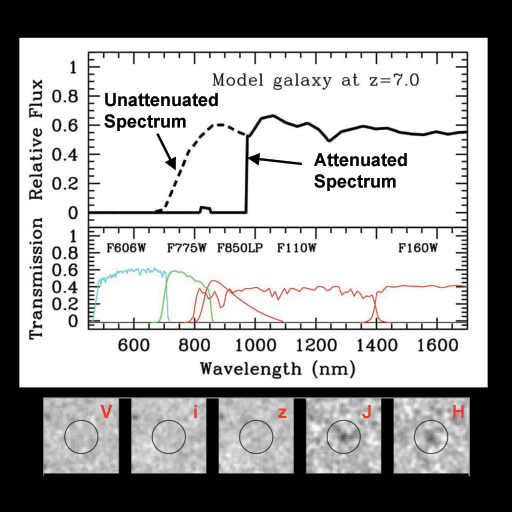
\includegraphics[width=0.5\textwidth]{../Images/drop_out_at_z7.png}
			\caption{Dropout technique for model redshift 7 galaxy\cite{first_galaxies_dropout_at_z7}.\label{fig:drop_out_at_z7}}
		\end{figure}

		The neutral hydrogen has attenuated almost all flux at wavelengths shorter than approximately 1 micrometre. The galaxy has been imaged in several different bands, and the longer wavelength filters show flux, whereas those at wavelengths corresponding to blue-ward of Lyman alpha do not. The galaxies that the group look to study have been shifted such that the drop happens in the infrared. The wavelength of the drop can be worked out using the known rest wavelength of Lyman alpha, as well as the factor by which the wavelength shifts due to the expansion of the universe, as shown in equation~\ref{eq:dropout_wavelength}.
		\begin{align}
			\text{Rest wavelength of Lyman alpha} \times (1+z) &= \text{observed wavelength of drop}\label{eq:dropout_wavelength}
		\end{align}

		Since the rest wavelength of Lyman alpha is known and the observed wavelength of the drop can be measured, the redshift of the galaxy can be determined. This
		is only a rough estimate when doing photometry since the flux is simply a number in each of the bands. For example, if the bands do not overlap, and the drop happens between two bands, it will not be known at what point the drop occurred, only the range in which it occurred. This motivates the use of bands which are close together or potentially even overlapping. Figure~\ref{fig:filter-systems} shows some different bands and their bandwidth, for different filter systems. Johnson-Cousins- Glass is one of the oldest and still the most commonly used system\cite{BasicObservationalKnowledge}.
		\begin{figure}[!htb]
			\centering
			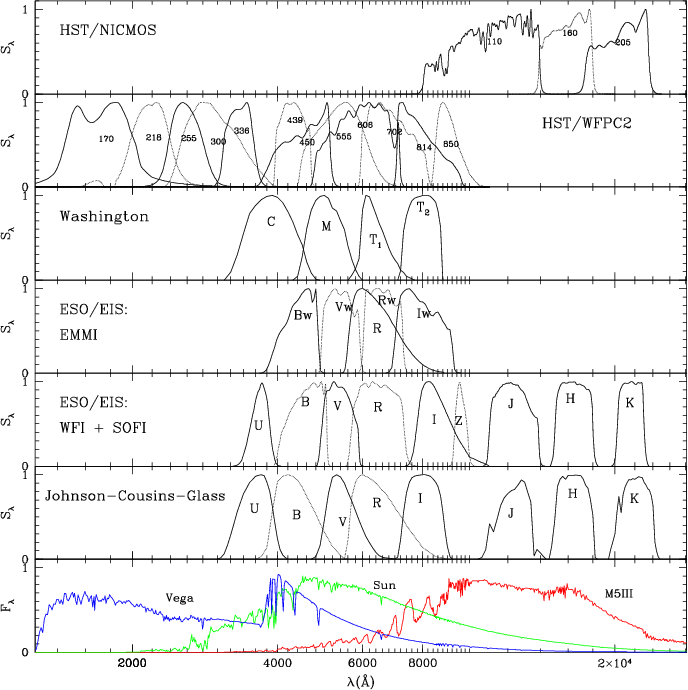
\includegraphics[width=0.65\textwidth]{../Images/filter-systems.png}
			\caption{Various filtering systems\cite{refId0}.\label{fig:filter-systems}}
		\end{figure}

		The bandwidth (or passband) is the wavelength range that can pass through the filter. Filters in different parts of the spectrum are given a common name, for example I band at \SI{806}{\nano\metre}. When observing LBGs, it is beneficial to have three filters in a row so that the position of the drop can be more accurately measured. As can be seen, there are gaps between the J H and K filters, meaning if the drop occurs between J and H, full flux should be observed in H and K and virtually no flux should be seen in J. (the panels beneath figure~\ref{fig:filter-systems} show an image (or lack thereof) of the $z=7$ galaxy in each of the V, I, z, J and H bands)

		Table~\ref{tab:filter_characteristics} below shows a list of filter names, the central wavelength of that filter, the bandwidth the filter covers, and range of redshifts for which the Lyman alpha drop would be covered. (This  range assumes the bandwidth covers 50\% either side of the central wavelength)
		\begin{table}[ht]
			\begin{center}
				\begin{tabular}{c|c|c|c}
					Filter 	& Central wavelength & Bandwidth & Redshift coverage \\
					\hline \hline
					V 	& \SI{551}{\nano\metre}	 & \SI{88}{\nano\metre} & 3.17--3.90 \\
					i 	& \SI{806}{\nano\metre}	 & \SI{149}{\nano\metre} & 5.01--7.25 \\
					Y 	& \SI{1020}{\nano\metre} & \SI{120}{\nano\metre} & 6.90--7.88 \\
					J 	& \SI{1220}{\nano\metre} & \SI{213}{\nano\metre} & 9.16--9.91 \\
					H 	& \SI{1630}{\nano\metre} & \SI{307}{\nano\metre} & 11.14--13.67 \\
					K 	& \SI{2190}{\nano\metre} & \SI{390}{\nano\metre} & 15.41--18.61
				\end{tabular}
			\end{center}
			\caption{Data highlighting which filters would be useful for observing particular redshift galaxies\cite{Galactic_Astronomy_Binney_Merrifield}}
			\label{tab:filter_characteristics}
		\end{table}

		Table~\ref{tab:filter_characteristics} must be taken into consideration that two filters should be red-ward of the drop and one blue-ward. One the fluxes have been measured in all three bands, if the object is indeed a LBG, there should be a sharp drop in flux in  one of the bands. However this does not totally rule out other possibilities: Some other objects could also exhibit a drop in flux, posing as LBGs, so usually a follow up method is used, and this is spectroscopy. Spectroscopy The drop out technique provides a good indication that a galaxy is a high redshift Lyman break galaxy, however the best way to confirm this is with spectroscopy. Spectroscopy involves\ldots

		At loads of different wavelengths, measure the spectra. Look for the drop

		Use ground based such as KECK or space based, JWST will have one.

		%JOHN IS DOING SPECTROSCOPY. I AM NOT NEEDED HERE.
		% subsection filters_and_the_dropout_technique (end)

% subsection determining_redshift (end)

    %!TEX root = mainfile.tex

\section{Other methods for detecting Re-ionization (21cm)} % (fold)
\label{sec:other_methods_for_detecting_re-ionization}

    \subsection{Hydrogen 21cm line} %fold
    \label{sub:Hydrogen_21cm}
        The method of using the hyperfine transition of neutral Hydrogen from the ground state to study re-ionization could provide much more detail about the process of re-ionization than the Lyman break dropout method.

         \subsubsection{Hyperfine transition of Hydrogen} %fold
         \label{subsub:Hyperfine_Hydrogen}
            The Hyperfine transition corresponds to the change in the two hyperfine levels of the hydrogen 1s ground state with an energy difference of \SI{5.87433}{\micro\electronvolt}.

            FURTHER RESEARCH FROM BOOK AND DIAGRAM
        %subsubsection Hyperfine_transition_of_Hydrogen (end)

        \subsubsection{Method of Measuring \SI{21}{\centi\metre}} %fold
    	\label{subsub:Measuring_21cm}
            To observe the hydrogen \SI{21}{\centi\metre} absorption spectrum, radio sources are needed. If the radio source is located before or during the epoch of re-ionization, it's possible to see the structure of neutral hydrogen gas along the line of sight using the absorption of the \SI{21}{\centi\metre} line in the radio spectrum. Several features should be apparent blueward of the redshifted \SI{21}{\centi\metre} line: a decrement of flux due to the optical depth of the IGM along the line of sight at a particular redshift, which will vary along the line of sight due to changes in density and the ionization of the IGM and there will be areas of transmission and absorption due to `bubbles' of photoionized hydrogen and dense areas or clouds of hydrogen. Currently there are several arrays of radio telescopes planned for observing the 21cm. LOFAR, GMRT, EDGES, PAPER, MWA, SKA.
        %subsubsection Measuring_21cm (end)

        \subsubsection{Advantages/disadvantages} %fold
    	\label{subsub:Advantages_disadvantages_21cm}
            The major advantage of observing the \SI{21}{\centi\metre} forest over the Lyman break technique is that it is possible to study the history of the re-ionization far more accurately, this is because the Gunn Peterson trough reaches zero flux for the lyman break technique with only a small fraction of hydrogen in the line of sight needed.

            The main reason this study did not use the \SI{21}{\centi\metre} absorption spectrum is that it requires far more careful consideration of the IGM. This is quite a different setup from the broad assumptions that can be made for the lyman break technique, and therefore it was thought that with the time constraint of the project. MORE NEEDED HERE
        %subsubsection Advantages_disadvantages_21cm(end)

    %subsection Hydrogen_21cm (end)

    \subsection{Other methods (tbc)} %fold
    \label{sub:Other_Methods_Re-ionization}

    %subsection Other_Methods_Re-ionization (end)

%section other_methods_for_detecting_re-ionization (end)

    %!TEX root = mainfile.tex

\subsection{CMB Secondary Anisotropies} % (fold)
\label{sub:cmb_secondary_anisotropies}
	Over large angular scales, the CMB polarization contains key information concerning the evolution of ionization during the EoR. The CMB photons released during recombination experienced considerable Thomson scattering off of free electrons. This scattering is imprinted onto the CMB anisotropy map introducing secondary anisotropies. This has the effect of removing anisotropies on smaller scales and introducing polarization anisotropies. By comparing the anisotropies observed with models of the CMB without reionization it is possible to determine the electron column density during the EoR. Using this method it is possible to calculate the period over which reionization took place. It is also possible to make measurements of the metal enrichment history of the IGM at the EoR. On-resonance scattering off metals and the influence of inverse Compton scattering (the Sunyaev-Zel'dovich effect) introduced additional signals into the CMB\cite{Monteagudo2006}. Studies in this field are expected to get a new impetus in the coming years with the results from the Planck telescope giving greater insight into the CMB map.
% subsection cmb_secondary_anisotropies (end)

    %!TEX root = mainfile.tex
\subsection{Spectroscopy} % (fold)
\label{sec:spectroscopy}
	The spectrum of typical high redshift galaxy can be seen in Figure~\ref{fig:high_redshift_galaxy_spectrum}.
	\begin{figure}[!htbp]
		\centering
			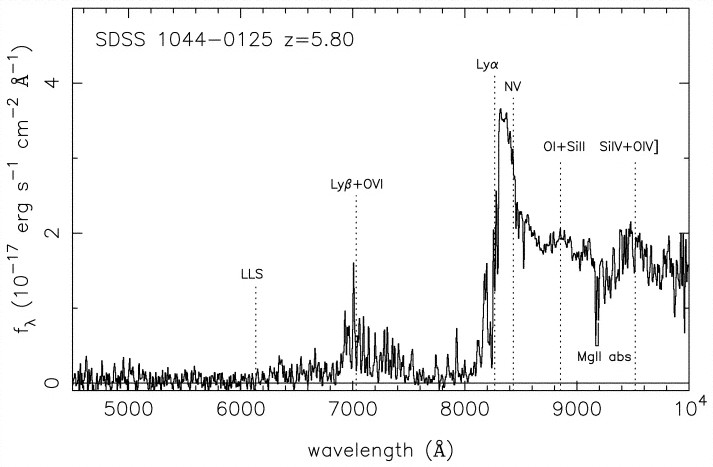
\includegraphics[width=0.7\textwidth]{../Images/high_redshift_galaxy_spec.jpg}
		\caption{\label{fig:high_redshift_galaxy_spectrum}}
	\end{figure}

	The distinct drop in emission is due to the presence of neutral hydrogen around the galaxies, known as the Gunn Peterson trough. Therefore the galaxies where formed before the start of re-ionisation. This is discussed in detail in Section~\ref{sec:the_gunn_peterson_effect}. However this particular feature in the spectra is of great importance here. The wavelength at which this drop occurs corresponds to the amount of energy required for an electron to transition between the first two energy levels in neutral hydrogen. This is known as the Lyman-$\alpha$ transition line and has a rest frame wavelength here on earth of \SI{1216}{\angstrom}\cite{rauch2001lyman}. However, the actual wavelength that this drop occurs in the spectrum of the galaxy being studied will be much longer. In Figure~\ref{fig:high_redshift_galaxy_spectrum}, it is closer to \SI{8000}{\angstrom}.This is due to the fact that the light is red shifted effectively stretching the wavelength. Indeed, the observed wavelength of the Lyman-$\alpha$ transition line will be in the infrared range. If this wavelength can be measured precisely then the redshift of the galaxy can be calculated\cite{rauch2001lyman}. This is done using the relation,
	\begin{align}
		1+z &= \frac{\lambda_{\text{observed}}}{\lambda_{\text{emitted}}} \label{eq:spectroscopy}
	\end{align}
	Hence, spectroscopy can be used to confirm the high-red shift galaxy candidates that are identified via photometry. In essence it is high resolution photometry.

	An astronomical spectrograph splits or disperses light from a source into its constituent wavelengths. Therefore it has to have some means of dispersing the light. The simplest way this can be achieved is via a prism. This exploits the fact that different wavelengths are diffracted via different amounts. However, they are rarely used by themselves in astronomical spectroscopy due to their inefficiency. Only about 10\% of the light incident upon them actually gets dispersed. Moreover, the dispersion is nonlinear causing some light to be dispersed more than others. Therefore, the universal dispersing medium used in astronomical spectroscopy is the diffraction grating. A diffraction grating consists of a large number of equidistant parallel lines ruled onto a transparent glass plate. The incident light cannot travel through the grating, but is instead channelled along the parallel lines. As the light reaches the end of the lines it is diffracted producing a series of wavelets in accordance with Huygens’s Principle. These either constructively or destructively interfere producing a series of maxima or minima. Again, different wavelengths of light will be diffracted through different angles. Therefore each maximum (order) can be thought of as the image of the galaxy split into its constituent wavelengths. As a general rule, the first maximum is projected onto the CCD equipment of the telescope and used to calculate the redshift. This is due to the fact it has the highest intensity. Figures~\ref{fig:grating_to_split_light} and~\ref{fig:grating_close_up} below show a schematic of a grating being used to split light
	\begin{figure}[!htbp]
		\begin{minipage}[c]{0.5\linewidth}
			\centering
			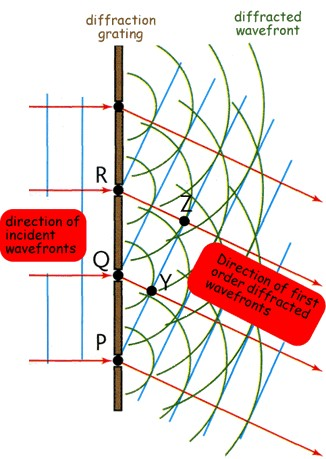
\includegraphics[width=0.7\textwidth]{../Images/grating_to_split_light.jpg}
			\caption{\label{fig:grating_to_split_light}}
		\end{minipage}
		\begin{minipage}[c]{0.5\linewidth}
			\centering
			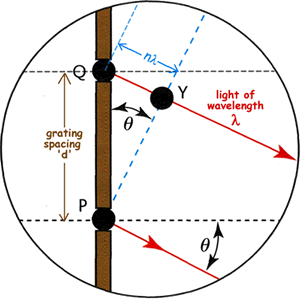
\includegraphics[width=0.7\textwidth]{../Images/grating_close_up.png}
			\caption{\label{fig:grating_close_up}}
		\end{minipage}
	\end{figure}

	Angles at which the orders occur can be found using the grating equation,
	\begin{align}
		n\lambda &= d(\sin\theta + \sin\phi)
	\end{align}
	Where $\phi$ is the angle of incidence between the light and the grating, $\theta$ is the angle of dispersion and $d$ is the grating spacing. The value of $n\lambda$ is an integer number of wavelengths of the incident light.

	Before light reaches either a prism or diffraction grating it is often sent through a fixed slit. This is a mask with a narrow rectangular aperture that is placed in the focal plane of the telescope. The slit has two main functions. First and foremost it isolates a portion of the sky of interest so that only light that falls on the slit may enter the spectrograph. This is important as it means the spectra from different parts of a galaxy cannot enter the spectrograph, overlap and thus contaminate each other. Second, the slit provides a stable spectral resolution. Without the slit the spectral resolution would be defined by the width of the galaxy or star. However, this varies with time so the spectral line width would vary with time. This would make detailed analysis of the spectrum almost impossible. If on the other hand a slit is used, the spectrum becomes an infinite number of images of the slit, and not the galaxy or star etc. As the slit width is constant, the spectral resolution remains stable.

	In between the slit and dispersion medium usually sits a collimator. The light from the slit diverges and if left would hit the grating or prism at differing angles of incidence making the resulting spectrum useless. Therefore a collimator is used to turn the diverging light back to parallel. Figure~\ref{fig:nirspec_jwst} below shows the set-up for NIRspec on the JWST.
	\begin{figure}[!htbp]
		\centering
			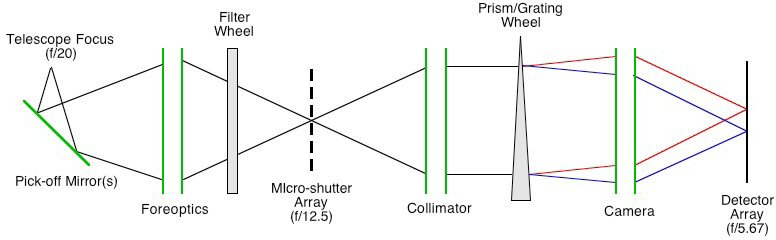
\includegraphics[width=0.8\textwidth]{../Images/nirspec_jwst.jpeg}
		\caption{\label{fig:nirspec_jwst}}
	\end{figure}

	Grisms are a combination of both diffraction gratings and prisms. In some cases they enable spectroscopy and photometry to be undertaken simultaneously. This is achieved by using the dispersed and undispersed light that they produce. This means that exposure times can be shortened when viewing and confirming high red shift galaxy candidates.
% section spectroscopy (end)


    %!TEX root = mainfile.tex

\subsection{Observational Gravitational Lensing} % (fold)
\label{sec:observational_gravitational_lensing}
	Gravitational lensing will enhance the observing capabilities of any telescope used allowing some of the most distant objects in the universe to be seen. Since one of the aims of this project is to push current boundaries and observe objects at as yet unexplored redshifts, lensing will prove to be a very useful tool. Lensed sources at redshifts above 7 tend to be magnified by a factor of 5 to 10 over an area of 1 square arcminute, however this magnification can be as much as 30 times for certain source locations\cite{magnification}. Two routes were considered to include gravitational lensing in the observing strategy: either new lenses could be located or lenses found by other surveys could be selected. This section lays out the properties desired for the lenses chosen and the arguments for each of these options.

	\subsubsection{Constraints on the Lenses} % (fold)
	\label{sub:constraints_on_the_lenses}
		The lenses used will be chosen depending on the suitability of their properties for the observing strategy. Firstly, the area of the sky in which the lenses lie must be chosen carefully, particularly if a ground based telescope is used. The region of sky must be chosen to be compatible with the direction in which the telescope(s) used for the deep survey are able to point. For a space based telescope, this is not a major issue since they are not confined by the Earth’s motion. Any regions with bright foreground contaminants would be ruled out and the lenses would be chosen such that they are distributed across the sky in order to reduce the effect of cosmic variance. Another factor that must be accounted for is that the lensing cross section of an object is directly dependent on its mass, as shown in Figure~\ref{fig:Lensing_cross_section_as_a_function_of_mass}\cite{Optimal_mass_configurations}. This would suggest that the lenses chosen should be very massive and are therefore likely to be galaxy clusters.
		\begin{figure}[!htbp]
			\centering
				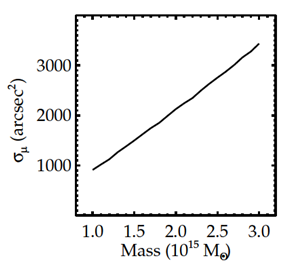
\includegraphics[width=0.4\textwidth]{../Images/Lensing_cross_section_as_a_function_of_mass.png}
			\caption[Lensing cross section as a function of mass]{\cite{Optimal_mass_configurations}Plot of the lensing cross section as a function of mass for a spherical halo at $z=0.5$. The dependence of cross section on mass can be clearly seen, indicating that the more massive a cluster, the better a lens it will be.\label{fig:Lensing_cross_section_as_a_function_of_mass}}
		\end{figure}

		The source magnification is also sensitively dependent on the lens redshift, though constraining this is less straightforward as there is a trade-off between Einstein angle and shear. On the one hand, the Einstein angle, an indicator of the strength of a lens, increases as the lens redshift decreases. Figure~\ref{fig:Einstein_angle_as_a_function_of_source_redshift} shows how lens redshift varies with Einstein angle. The point at which each curve crosses the x-axis is the lens redshift, since no lensing occurs when the source and lens redshifts are equal. For each value of lens redshift, the Einstein angle increases rapidly at source redshifts slightly greater than that of the lens, and then quickly saturates\cite{Constraining_source_redshift_distributions}. The lower the redshift of the lens, the higher the saturation value, suggesting lower lens redshifts are the best.
		\begin{figure}[!htbp]
			\centering
				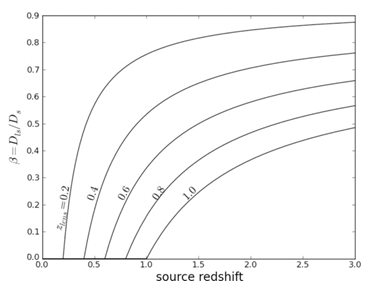
\includegraphics[width=0.5\textwidth]{../Images/Einstein_angle_as_a_function_of_source_redshift.png}
			\caption[Einstein angle as a function of source redshift]{\cite{Constraining_source_redshift_distributions} Plot of Einstein angle against source redshift. Again, each line corresponds to a different lens redshift. The point at which each line crosses the x-axis is the lens redshift, since at the lens, the magnification of the source is equal to 0.\label{fig:Einstein_angle_as_a_function_of_source_redshift}}
		\end{figure}

		However, the extent to which the images are distorted is not taken into account. The shear caused by a lens at a particular redshift is given by
		\begin{align}
			\gamma(r) &= \frac{4\pi G}{c^2}\frac{D_{LS}D_L}{D_S}\left( \overline{\Sigma}(<r)-\Sigma(r) \right)
		\end{align}
		where $\overline{\Sigma}(<r)$ is the mean projected surface mass density within r and $\Sigma(r)$ the projected surface mass density at $r$. Keeping the radius (and therefore surface mass density) constant, Figure~\ref{fig:shear_as_a_function_of_source_redshift} shows the dependence of shear on source redshift at the same fixed lens redshifts as the plot above. lens redshifts as the plot above. It can be seen from this plot, that at low source redshifts, the shear distortion is immeasurably small. As the redshift increases to around 0.5, the clusters at the lowest redshifts cause some significant distortion. Once the source redshift is greater than 1, shear distortion is seen around clusters at all the lens redshifts plotted\cite{Constraining_source_redshift_distributions}.
		\begin{figure}[!htbp]
			\centering
				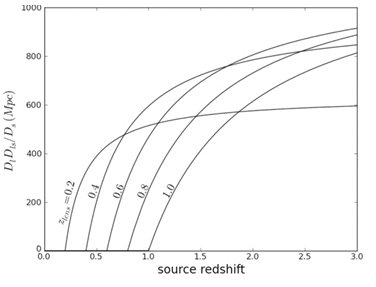
\includegraphics[width=0.5\textwidth]{../Images/Shear_as_a_function_of_source_redshift.png}
			\caption[Shear as a function of source redshift]{\cite{Constraining_source_redshift_distributions}A plot of shear against source redshift, with each line representing a different lens redshift. The point at which the lines cross the x-axis is the lens redshift, since at the lens, the magnification of the source is equal to 0.\label{fig:shear_as_a_function_of_source_redshift}}
		\end{figure}

		It has also been found that giant arcs are most likely to form behind higher redshift lenses, as shown in Figure~\ref{fig:Arc_probability}. Giant arcs are observed in systems where the shear is large. Lensing clusters at a redshift above 0.5 have been found to have an arc formation probability up to 3 times that of lower redshift lenses. Clusters observed at $z>0.5$ have also been found as a general rule to be less massive than closer clusters, indicating that clusters at this redshift are more efficient lenses. As a result, a judicious choice of lens redshift must be made to optimise both lensing strength and distortion for the best chance of observing high redshift galaxies\cite{wu_and_chiueh}.
		\begin{figure}[!htbp]
			\centering
				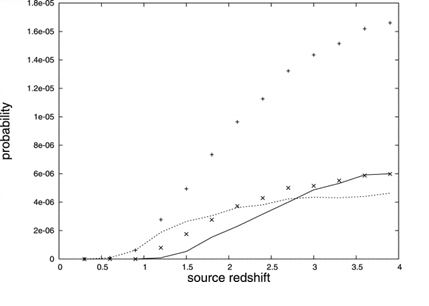
\includegraphics[width=0.5\textwidth]{../Images/Arc_probability.png}
			\caption[Arc probability]{\cite{wu_and_chiueh}Plot of the arc probability against source redshifts in four different lens intervals, $0.14\le z_L\le 0.45$ (dotted line), $0.49\le z_L\le 0.68$ (crosses), $0.73\le z_L\le 0.94$ (solid line), and $0.14\le z_L\le 0.94$ (plus signs).\label{fig:Arc_probability}}
		\end{figure}
	% subsection constraints_on_the_lenses (end)

	\subsubsection{Locating New Lenses} % (fold)
	\label{sub:locating_new_lenses}
		Locating new lenses would be advantageous in that the lenses could be chosen with the tight constraints specified above such that their properties are tailored to suit the needs of our strategy. The lenses would be selected using some form of wide survey by means of their strong lensing properties since objects that lense strongly are likely to be better for observing very faint sources. The parameters describing the lenses located would not be known so calculations to find these must be carried out. Taking the Einstein radius to be the average distance of the arcs from the centre of the lens, and assuming that most of the mass of the cluster is enclosed within this radius, an estimate of the mass can be found from
		\begin{align}
			M &= \Sigma_c\pi \theta_E^2 \label{eq:new_lens_mass_estimate}
		\end{align}
		The critical surface density, as defined in equation~(\ref{eq:new_lens_mass_estimate}) can be found when the source redshift is known and the magnification of the source can then be calculated as detailed in Section~\ref{sec:gravitational_lensing}.
	% subsection locating_new_lenses (end)

	\subsubsection{Using Known Lenses} % (fold)
	\label{sub:using_known_lenses}
		The second option, selecting known lenses has the advantage that the masses and velocity dispersions would already be well determined, allowing an accurate calculation of the magnification to be made. Examples of surveys that have been carried out previously include the Cluster Lens And Supernova survey with Hubble (CLASH)\cite{CLASH} and the MAssive Cluster Survey (MACS)\cite{MACS}. There are only a limited number of massive clusters known, however even with the small sample available, many interesting sources have already been observed for example a candidate $z\approx11$ galaxy behind cluster MACSJ0647.7+7015\cite{CLASH_z11_candidate}. Unless a wide survey is carried out as part of the observing strategy, using known lenses would significantly reduce the observing time required for the strategy compared to requiring an additional survey to locate new lenses. Both MACS and CLASH select their source using x-rays in order to obtain an unbiased distribution of masses, however, for this strategy the lenses would be chosen from these catalogues based on their masses and lensing properties.

	% subsection using_known_lenses (end)
% section observational_gravitational_lensing (end)

    %!TEX root = mainfile.tex

\subsection{Decision on Detection Techniques} % (fold)
\label{sec:decision_on_detection_techniques}
	Following the discussion of the observational techniques available, it has been decided that the CMB anisotropy and the \SI{21}{\centi\metre} line will not be used. Studying the CMB anisotropy is very useful for calculating the timescale of reionization and understanding the earliest moments. However, in this project we are looking to further the knowledge of the EoR with new observational data across the whole of the epoch and alternative methods are set to advance faster than using the CMB due the influx of new technology. The \SI{21}{\centi\metre} line offers much promise for expanding our understanding of the EoR and accurately mapping the evolution of the hydrogen distribution. Projects investigating the \SI{21}{\centi\metre} line so far have had limited success due mostly to the vast amounts of radio interference around the Earth, especially in the ionosphere. There are a number of planned projects, such as the Square Kilometre Array, seeking to further achievements in this field but with limited success so far we feel it is best to look at techniques that can be emulated and advanced upon.

	The strategy we propose will consist of the following:
	\begin{itemize}
		\item The first phase will consist of a low redshift survey capable of detecting LBGs from a redshift range of approximately $z=6-10$. This is approximately where current limits can see up to but with the advances in technology we believe that a new map over this period can provide even greater insight and constrain the evolution of the neutral hydrogen fraction.
		\item The next phase of our strategy will consist of a high redshift survey capable of finding galaxies at redshifts of 10 and higher. As stated, our aim is to see further back than previously achieved; this will require long survey times because of the low apparent magnitudes of these galaxies. There has already been some success in this area with the HUDF, as discussed in Section~\ref{ssub:achievements_to_date} and with a host of new telescopes being readied for the next generation of study the chance to see even further is an exciting prospect. This survey will look to include the use of known gravitational lenses to magnify distant galaxies and observe redshifts otherwise beyond our observational limits.
		\item Spectroscopy is the only real way of getting a confirmation of the galaxies' composition and true redshift. There are currently many candidates for LBGs that have been identified but are awaiting confirmation from spectroscopic analysis. Spectroscopically confirming a subset of the galaxies discovered across all redshifts will constitute the final phase of the project. There are a number of new and more advanced spectrometers planned for launch in the next 5--10 years which will be capable of performing this. The strategy will be structured to allow spectroscopy and photometry to run concurrently when possible.
	\end{itemize}
% section decision_on_detection_techniques (end)

    %!TEX root = mainfile.tex

\section{Photometry and Colour} % (fold)
\label{sec:Photometry_Colour}
	Photometry today is used primaily with CCDs, which can convert the transmitted flux into an electric signal which can then be interpretted as a magnitude. The magnitude system used in this project was the AB magnitude system as outlined in Section~\ref{ssub:ab_magnitude}.

	In this project wide and intermediate filters have been used predominantly. A common method for making these filters is to use coloured glass which either pass all light above a certain wavelength or pass all light up to a certain wavelength, these are known as cutoff filters. A bandpass filter can be made by combining two types of coloured glass, one which will act as the low wavelength cutoff and the other as the high wavelength cutoff. Filters don't transmit 100\% of the wavelengths that are allowed to pass, and the cutoff isn't at an exact frequency.

	To detect lyman-break galaxies the dropout method is used, which uses at least three filters to get enough spectral information to identify the object as a candidate for being a lyman break galaxy (see dropout method Section~\ref{ssub:dropout_technique}). However, observing the drop due to the Gunn-Peterson effect is not enough to confirm the identities of these candidates, other observational methods need to be used to be certain the object is a lyman break galaxy and not a contaminant. One of the most effective ways of eliminating contaminants is to use the colour of the object between different filters, obtained from the photometric measurements. The filters for each telescope were decided by determining where the lyman-break wavelength would appear at a certain redshift, using the equation,
	\begin{align}
		z=\frac{{{\lambda}_\text{obs}}-{{\lambda}_\text{emit}}}{{{\lambda}_\text{emit}}}
	\end{align}
	and finding which filter would contain this wavelength. The two filters either side of this filter were chosen as well for colour observations and for the dropout technique. The table below shows the filters used for various red shift ranges, with the filter in the middle of each redshift range being the filter where the lyman break would be observed. Note that the James Webb telescope and Euclid are the only telescopes shown because they were the telescopes chosen for the strategy.
	\begin{table}[ht]
		\centering
			\begin{tabular}{c|c|c}
				Redshift range &Telescope &Filters   \\
				\hline \hline
				6-7.5	   &James-Webb&  F070w, F090w, F115w \\
				7.5-8.5&James-Webb&  F090w, F115w, F150w \\
				8.5-10 &Euclid&  Y, J, H\\
				10-14  &James-Webb& F115w, F150w, F200w\\
				14-15  &0.105& F150w, F200w, F277w\\
			\end{tabular}
		\caption{Table showing filters used for different redshift ranges}
		\label{tab:colour_filters}
	\end{table}.


    \subsection{Contaminants} %fold
    \label{sub:Contanimants}
    	\subsubsection{Sources of Contamination} % (fold)
    	\label{ssub:sources_of_contamination}
    	%Need to be one level lower, may change

		    \subsubsection*{Low Mass Stars} % (fold)
		    \label{sub:low_mass_stars}
		        These can easily be identified due to the high resolution imaging provided by JWST and Euclid. The Point-spread function (PSF) obtained will allow us to determine which sources are point-like and which are extended. We should be able to avoid significant contamination by removing any point-like sources from the results as all galaxies should have a great enough diameter.
		    % subsection low_mass_stars (end)

		    \subsubsection*{Spurious Sources} % (fold)
		    \label{sub:spurious_sources}
		        By stipulating that we will be requiring detections in two bands the influence of spurious sources will be negligible. Finding detections in 2/3 bands at reasonable confidence interval ($S/N =5$) is very improbable. By inspecting the negative with the same requirements for detection we are able to easily identify any such sources.\cite{Bouwens2011}.
		    % subsection spurious_sources (end)

		    \subsubsection*{Supernovae and other transient sources} % (fold)
		    \label{sub:supernovae_and_other_transient_sources}
		        Events such as Supernovae happen incredibly quickly releasing a vast amount of energy, as seen in Figure~\ref{fig:SNe_1987a}. These events can spoil images due to their short duration by introducing new data in only a portion of the sample. These effects are usually only considered when taking exposures years apart or when combining multiple sources over a long time scale. Such events are very unlikely to contaminate our results as we propose to take our images close in time.
		        \begin{figure}[htbp]
		            \centering
		            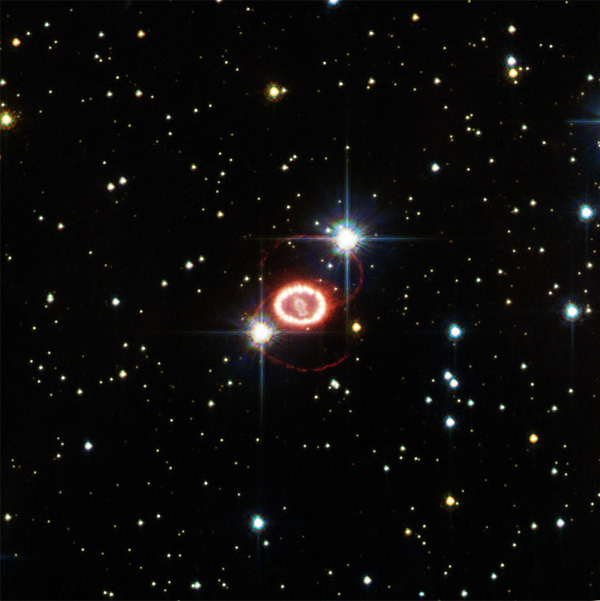
\includegraphics[width=0.6\textwidth]{../Images/SNe_1987a.jpg}
		            \caption{The shock wave from Supernova 1987a imaged by HST in 2006.\label{fig:SNe_1987a}}
		        \end{figure}
   			 % subsection supernovae_and_other_transient_sources (end)

		    \subsubsection*{Lower Redshift Sources and photometric scattering} % (fold)
		    \label{sub:lower_redshift_sources_and_photometric_scattering}
		        This category is likely to provide the greatest source of contamination for the surveyed area. It will do so increasingly at high redshifts where its affect on the faintest magnitudes is most greatly felt. Its affect is most influential with a small S/N ratio for the observations, by fixing this at a level of $S/N = 5$ we can be confident that the contamination will be low. Detecting a source in another band such as b435, v606, i775 for YJH photometry would class it as a contaminant and then should be removed from sample, however we wont use this as it would too greatly increase the time.
		    % subsection lower_redshift_sources_and_photometric_scattering (end)

    	% subsubsection sources_of_contamination (end)
    	\subsubsection{Eliminatiing Contaminants} % (fold)
    	\label{sub:eliminatiing_contaminants}
			The \emph{colour} of an object in photometry is defined as the difference in magnitude between two filters\cite{Romanishin}. If there are two filters, for example purposes let them be called A and B, where A has a lower central wavelength, the colour for an object in these two filters would be,
			\begin{align}
				m_A-m_B=-2.5\log\left(\frac{f_A}{f_B}\right).
			\end{align}
			where $f_A$ and $f_B$ are the specific flux denisites of the filters A and B\cite{Romanishin}. The colour is therefore equivalent to the ratio of specific flux densities, this means two objects with the same colour can have different magnitudes in each of the filters. If the colour is positive it is said to be `red' and if it is negative it is said to be `blue', i.e. an an object which is red between two filters has a lower flux in the blueward filter compared to the redward filter and an object which is red has a larger flux in the blueward filter than the redward one.  The larger the value is, it is said that the `redder' the object is. To eliminate contaminants from observations, a colour-colour diagram can be made using three filters, with two colour values for each object. For instance if the observations were done in the J, H and K filters, the colour colour diagram would be (H-K) plotted against (J-H). Although this study does not take any observtions, colour diagrams can be built up for observations by simulating a catalog of lyman break galaxies at high redshift and determine colour windows for observations using the program Hyperz. Lyman-break galaxies are very red in colour for the filter blueward of the break and over the break due to the extreme drop in flux blueward of the lyman-break, and they will be a low red value or even blue value for the colour between the filter over the break and redward of the break, due to the decrease in flux past the break. In this way contaminants as described in Section~\ref{sec:contaminants} can be removed quickly from observations.
    	% subsection eliminatiing_contaminants (end)
	%subsection Eliminating_Contaminants (end)
% section contaminants (end)

    \subsection{Hyperz} %fold
	\label{sub:Hyperz}
		To eliminate contaminates and predict colour windows for observations the program Hyperz and its subprogram `make\_catalog' can be used to produce a catalog of synthetic galaxies and their magnitudes in different filters at different redshifts.

        \subsubsection{Inputs} %fold
        \label{subsub:Hyperz_inputs}
			To produce this catalog, a set of inputs are put into the catalog file. The operation of the program is quite complex and is only summarised here. Also, the operation of make catalog is slightly different to Hyperz and a full manual for make catalog was not obtainable. The program starts with a sample Spectral Energy Distribution (SED), which has key features such as the lyman-break which will appear as the redshift is increased, the program combines this with a sample burst spectrum, which assumes the stars formed quickly, which is a good assumption for high redshift galaxies\cite{hyperz}. The Predictions group schecter function used the \SI{1500}{\angstrom} rest UV wavelength with the assumption that the flux from a lyman break galaxy was approximately the same for \SI{1350}{\angstrom} to \SI{1750}{\angstrom}. The program uses a known magnitude in a reference filter to fit the SED and to find the magnitde of the object in other bands. Using the Prediction's group program, a range of magnitudes can be found for a certain redshift interval by looking at the number of galaxies for a certain magnitude at a certain redshift. As the redshifted \SI{1500}{\angstrom} line will move with redshift, a range of reference filters were required to cover the redshift range for the observing strategy. As the flux is assumed to be constant over the range \SI{1350}{\angstrom}--\SI{1750}{\angstrom}, this meant a single filter could be used for a wide interval of redshifts. The reference filters were chosen to have a central wavelength as close to the central \SI{1500}{\angstrom} wavelength for that redshift. The reference magnitudes were based upon the predictions program for calculating the number density of galaxies. For each redshift range a lower magnitude was chosen based on whether any galaxies were observed below the chosen magnitude. The maximum magnitude was chosen to 35, as this was the limit the observing strategy had chosen to use. The reference magnitude ranges are therefore different sizes, and this is perhaps not wise to be able to compare similar redshifts, further consideration of reference magnitudes would have been desirable. Below is a table listing the reference filters used. Note that filter 44 was not correctly labelled in the database of filters! This created unforseen problems for the Euclid magnitudes and it wasn't apparant for a long time that the reference filter was to blame.
			\begin{table}[ht]
				\begin{center}
					\begin{tabular}{c|c|c}
						Redshift range & reference filter number&reference magnitudes \\
						\hline \hline
						6-7.5	   &34&27-35\\
						7.5-8.5&55&27.5-35\\
						8.5-10 &44&28-35\\
						10-14  &35&29-35\\
						14-15  &72&30-35\\
					\end{tabular}
				\end{center}
				\caption{Table showing reference filters and magnitudes used}
				\label{tab:reference_filters}
			\end{table}.

			There are several other inputs which are easy to understand: the user chooses the range of redshifts for the catalog, the formation redshift, which is when the galaxies started forming and to keep consistency between the two groups, the same cosmological constants were used as the predicitons group, which were: $\Omega_M=0.27$, $\Omega_\Lambda=0.73$ and $H_0=\SI{71}{\kilo\metre\per\second\per\mega\parsec}$. Two other parameters which are slightly more complex are the age of the galaxies and the reddening law. To simplify the calculations, the age of the galaxies was set such that galaxies at the same redshift have the same age, forming at the same moment at the formation reshift. The other choice for the galaxies to be born somewhere randomly between the formation redshift and the observed redshift. The reddening law is a more detailed input and is considered below.
		%subsubsection Inputs (end)

		\subsubsection{Reddening Law} % (fold)
		\label{ssub:reddening_law}
			Hyperz can account for Reddening of galaxies. Reddening refers to the SED of a galaxy appearing redder than it actually is and is one of the effects due to the prescence of dust. Dust is matter within galaxies that inteferes with the photons travelling towards the observer. Through spectral analysis, it has been determined that dust is composed of substances such as Carbon, silicate materials, water and ammonia in the form of ice amongst other substances \cite{stein1983dust}. Dust can absorb (and emit) photons, with absorbtion occuring most in the UV and therefore the spectrum appears reddened\cite{stein1983dust}. Hyperz allows the user to select one of five laws to apply to the catalogs produced, and the law that was chosen for the purposes of this study was the Calzetti et al. (2000). There were two reasons for this: it seems to be the law that most recent papers use and appears to be a more general approximation than other laws which are based on specific galaxies and it is a law for starburst galaxies, which corresponds to the sample spectrum used. The program asks for a maximum and minimum value of extinction in terms of magnitude, defined as $A_V$. Several steps are required to get to this required value. Starting with the equation
			\begin{align}
				A_\lambda=k(\lambda)E(B-V)=\frac{k(\lambda)A_V}{R_V}
			\end{align}
			where $A_\lambda$ is defined as the extinction at a certain wavelength, $k(\lambda)$ is the reddening curve, E(B-V) is the colour excess and $R_V$ is a constant \cite{hyperz}. The equation can be arranged to find $A_V$,
			\begin{align}
				A_V=\frac{k(\lambda)A_\lambda}{R_V}.
			\end{align}
			$R_V$ is given as $4.05 {\pm} 0.8$ \cite{hyperz} for the Calzetti law and
			\begin{align}
				k(\lambda)=2.659(-1.857+\frac{1.040}{\lambda})+R_V
			\end{align}
			for $0.12{\mu}m \le \lambda \le 0.63{\mu}m$ for the Calzetti law\cite{hyperz}. $\lambda$ is assumed to be the emitted wavelength from the galaxy, which will be assumed to be 1216$\angstrom$ as an assumption to simplify the calculation. The only unknown is $A_\lambda$. From the equation
            \begin{align}
				f_{obs}(\lambda)=f_{int}(\lambda)10^{-0.4A_\lambda}
			\end{align}
			where $f_{obs}$ is the observed flux and $f_{int}$ is the intrinsic flux, which is the flux if no reddening occured\cite{hyperz}. It can be seen that if $A_\lambda=0$ then there is no reddening, which leads to a value of zero for $A_V$. This can then be set for the minimum value for the Reddening law, although it will be very improabable for there to be no extinction, it is theoretically possibly and simplifies the situation. the maximum value for $A_V$ is harder to find as this project doesn't take any observations and the program from the predictions group gives intrinsic fluxes, so values were found using NED's Coordinate and Galactic Extinction Calculator\cite{NEDex}. Using a set of galaxies from various papers in a redshift range of 6--9, their Right Ascension and Declination were inputted into the calculator, which then found values of $A_\lambda$ for a range of filters. For each redshift the filter chosen contained the redshifted lyman break for those galaxies, the galaxy with the maximum extinction value was chosen for each redshift range. In the table below are the values obtained. For redshift 10--15 the data was extrapolated to find values. The maximum difference in $A_\lambda$ between redshifts was found for the known galaxies, and then this was applied for each increase in redshift.
			\begin{table}[ht]
				\begin{center}
					\begin{tabular}{c|c|c}
						Redshift range & $A_\lambda$ & $A_V$  \\
						\hline \hline
						6-7.5	   &0.013&  0.0044 \\
						7.5-8.5&0.013&  0.0044 \\
						8.5-10 &0.036&  0.0122\\
						10-14  &0.082&  0.0277\\
						14-15  &0.105&  0.0355\\
					\end{tabular}
				\end{center}
				\caption{Table showing values of Extinction for different redshift values}
				\label{tab:extinction_values}
			\end{table}.

			These values were put into the catalog. Many assumptions were made to find this value, so it may be incorrect. Articles tend to have a much bigger value for the maximum extinction, for example in the Hyperz manual it is 1.2. However the best possible figure was obtained with the resources avalaible. the extinction due to the Milky Way has not been considered which might have made a significant difference.
		% subsubsection reddening_law (end)

		\subsubsection{Vega to AB Conversions} % (fold)
		\label{ssub:vega_to_ab_conversions}
			Hyperz works in Vega magnitudes so AB conversions are needed. These conversions are complex and therefore conversions for a ground based telescope for typical filters have been used from\cite{Graham} Filters were compared to the nearest equivalent but some will inevitably be different from the actual values. The reference filters were from the database of filters that came with Hyperz and so came ready with conversions to AB. The conversions for the reference filters were applied for the input into the program, and the output magnitude in the various filters were changed to AB from Vega. The table below shows the conversion for each filter chosen for observation.
			\begin{table}[ht]
				\begin{center}
					\begin{tabular}{c|c}
						Filters & M(AB)-M(Vega) \\
						\hline \hline
						F070w, F090w,  & 0.5 \\
						F115w, Euclid Y, Euclid J	& 0.9\\
						 F150w, Euclid H	& 1.4\\
						F200w, F275w & 1.9\\
					\end{tabular}
				\end{center}
				\caption{AB conversions for filters}
				\label{tab:AB_conversion}
			\end{table}
		% subsubsection vega_to_ab_conversions (end)

		\subsubsection{Output} % (fold)
		\label{ssub:output}
			After running the executable file, the output is shown in a catalog, each redshift calaculated is random, so the galaxies are in a random order. From the output, the colour of an object can be found after the AB conversions have been made to the magnitudes and a colour diagram can then be plotted.
		% subsubsection output (end)
	%subsection Hyperz (end)

	\subsection{Results for Colour} %fold
	\label{sub:Results_for_Colour}
		Below are the results for four of the specified ranges, the redshift range 14 to 15 was not included here as there was an unresolved problem with the F275w filter on NIRcam, which will be discussed below. The colour windows were found by finding the minimum value of the y-axis and the maximum value of the x-axis and stating that the colour window must be greater than or equal to and less than or equal to the values on the axes respectively, isolating the upper left quadrant of each colour diagram to be the colour window.
		\begin{figure}[htbp]
			\begin{minipage}[c]{0.5\linewidth}
				\centering
					\begingroup\endlinechar=-1
						\resizebox{\textwidth}{!}{%
							% GNUPLOT: LaTeX picture with Postscript
\begingroup
  \makeatletter
  \providecommand\color[2][]{%
    \GenericError{(gnuplot) \space\space\space\@spaces}{%
      Package color not loaded in conjunction with
      terminal option `colourtext'%
    }{See the gnuplot documentation for explanation.%
    }{Either use 'blacktext' in gnuplot or load the package
      color.sty in LaTeX.}%
    \renewcommand\color[2][]{}%
  }%
  \providecommand\includegraphics[2][]{%
    \GenericError{(gnuplot) \space\space\space\@spaces}{%
      Package graphicx or graphics not loaded%
    }{See the gnuplot documentation for explanation.%
    }{The gnuplot epslatex terminal needs graphicx.sty or graphics.sty.}%
    \renewcommand\includegraphics[2][]{}%
  }%
  \providecommand\rotatebox[2]{#2}%
  \@ifundefined{ifGPcolor}{%
    \newif\ifGPcolor
    \GPcolortrue
  }{}%
  \@ifundefined{ifGPblacktext}{%
    \newif\ifGPblacktext
    \GPblacktexttrue
  }{}%
  % define a \g@addto@macro without @ in the name:
  \let\gplgaddtomacro\g@addto@macro
  % define empty templates for all commands taking text:
  \gdef\gplbacktext{}%
  \gdef\gplfronttext{}%
  \makeatother
  \ifGPblacktext
    % no textcolor at all
    \def\colorrgb#1{}%
    \def\colorgray#1{}%
  \else
    % gray or color?
    \ifGPcolor
      \def\colorrgb#1{\color[rgb]{#1}}%
      \def\colorgray#1{\color[gray]{#1}}%
      \expandafter\def\csname LTw\endcsname{\color{white}}%
      \expandafter\def\csname LTb\endcsname{\color{black}}%
      \expandafter\def\csname LTa\endcsname{\color{black}}%
      \expandafter\def\csname LT0\endcsname{\color[rgb]{1,0,0}}%
      \expandafter\def\csname LT1\endcsname{\color[rgb]{0,1,0}}%
      \expandafter\def\csname LT2\endcsname{\color[rgb]{0,0,1}}%
      \expandafter\def\csname LT3\endcsname{\color[rgb]{1,0,1}}%
      \expandafter\def\csname LT4\endcsname{\color[rgb]{0,1,1}}%
      \expandafter\def\csname LT5\endcsname{\color[rgb]{1,1,0}}%
      \expandafter\def\csname LT6\endcsname{\color[rgb]{0,0,0}}%
      \expandafter\def\csname LT7\endcsname{\color[rgb]{1,0.3,0}}%
      \expandafter\def\csname LT8\endcsname{\color[rgb]{0.5,0.5,0.5}}%
    \else
      % gray
      \def\colorrgb#1{\color{black}}%
      \def\colorgray#1{\color[gray]{#1}}%
      \expandafter\def\csname LTw\endcsname{\color{white}}%
      \expandafter\def\csname LTb\endcsname{\color{black}}%
      \expandafter\def\csname LTa\endcsname{\color{black}}%
      \expandafter\def\csname LT0\endcsname{\color{black}}%
      \expandafter\def\csname LT1\endcsname{\color{black}}%
      \expandafter\def\csname LT2\endcsname{\color{black}}%
      \expandafter\def\csname LT3\endcsname{\color{black}}%
      \expandafter\def\csname LT4\endcsname{\color{black}}%
      \expandafter\def\csname LT5\endcsname{\color{black}}%
      \expandafter\def\csname LT6\endcsname{\color{black}}%
      \expandafter\def\csname LT7\endcsname{\color{black}}%
      \expandafter\def\csname LT8\endcsname{\color{black}}%
    \fi
  \fi
  \setlength{\unitlength}{0.0500bp}%
  \begin{picture}(7200.00,4320.00)%
    \gplgaddtomacro\gplbacktext{%
      \put(747,595){\makebox(0,0)[r]{\strut{} 3}}%
      \put(747,1047){\makebox(0,0)[r]{\strut{} 3.5}}%
      \put(747,1500){\makebox(0,0)[r]{\strut{} 4}}%
      \put(747,1952){\makebox(0,0)[r]{\strut{} 4.5}}%
      \put(747,2404){\makebox(0,0)[r]{\strut{} 5}}%
      \put(747,2856){\makebox(0,0)[r]{\strut{} 5.5}}%
      \put(747,3309){\makebox(0,0)[r]{\strut{} 6}}%
      \put(747,3761){\makebox(0,0)[r]{\strut{} 6.5}}%
      \put(849,409){\makebox(0,0){\strut{} 3.5}}%
      \put(1453,409){\makebox(0,0){\strut{} 4}}%
      \put(2058,409){\makebox(0,0){\strut{} 4.5}}%
      \put(2662,409){\makebox(0,0){\strut{} 5}}%
      \put(3267,409){\makebox(0,0){\strut{} 5.5}}%
      \put(3871,409){\makebox(0,0){\strut{} 6}}%
      \put(4475,409){\makebox(0,0){\strut{} 6.5}}%
      \put(5080,409){\makebox(0,0){\strut{} 7}}%
      \put(5684,409){\makebox(0,0){\strut{} 7.5}}%
      \put(6289,409){\makebox(0,0){\strut{} 8}}%
      \put(6893,409){\makebox(0,0){\strut{} 8.5}}%
      \csname LTb\endcsname%
      \put(144,2178){\rotatebox{-270}{\makebox(0,0){\strut{}f070w-f090w}}}%
      \csname LTb\endcsname%
      \put(3871,130){\makebox(0,0){\strut{}f090w-f115w}}%
      \put(3871,4040){\makebox(0,0){\strut{}Redshift 6--7.5}}%
    }%
    \gplgaddtomacro\gplfronttext{%
    }%
    \gplbacktext
    \put(0,0){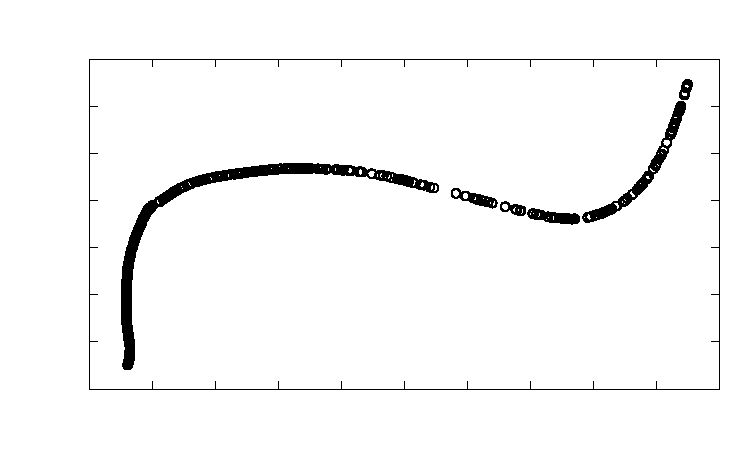
\includegraphics{GRAPH_color_graph1}}%
    \gplfronttext
  \end{picture}%
\endgroup

						}\endgroup
				\caption{A\label{fig:col1}}
			\end{minipage}
			\begin{minipage}[c]{0.5\linewidth}
				\centering
					\begingroup\endlinechar=-1
						\resizebox{\textwidth}{!}{%
							% GNUPLOT: LaTeX picture with Postscript
\begingroup
  \makeatletter
  \providecommand\color[2][]{%
    \GenericError{(gnuplot) \space\space\space\@spaces}{%
      Package color not loaded in conjunction with
      terminal option `colourtext'%
    }{See the gnuplot documentation for explanation.%
    }{Either use 'blacktext' in gnuplot or load the package
      color.sty in LaTeX.}%
    \renewcommand\color[2][]{}%
  }%
  \providecommand\includegraphics[2][]{%
    \GenericError{(gnuplot) \space\space\space\@spaces}{%
      Package graphicx or graphics not loaded%
    }{See the gnuplot documentation for explanation.%
    }{The gnuplot epslatex terminal needs graphicx.sty or graphics.sty.}%
    \renewcommand\includegraphics[2][]{}%
  }%
  \providecommand\rotatebox[2]{#2}%
  \@ifundefined{ifGPcolor}{%
    \newif\ifGPcolor
    \GPcolortrue
  }{}%
  \@ifundefined{ifGPblacktext}{%
    \newif\ifGPblacktext
    \GPblacktexttrue
  }{}%
  % define a \g@addto@macro without @ in the name:
  \let\gplgaddtomacro\g@addto@macro
  % define empty templates for all commands taking text:
  \gdef\gplbacktext{}%
  \gdef\gplfronttext{}%
  \makeatother
  \ifGPblacktext
    % no textcolor at all
    \def\colorrgb#1{}%
    \def\colorgray#1{}%
  \else
    % gray or color?
    \ifGPcolor
      \def\colorrgb#1{\color[rgb]{#1}}%
      \def\colorgray#1{\color[gray]{#1}}%
      \expandafter\def\csname LTw\endcsname{\color{white}}%
      \expandafter\def\csname LTb\endcsname{\color{black}}%
      \expandafter\def\csname LTa\endcsname{\color{black}}%
      \expandafter\def\csname LT0\endcsname{\color[rgb]{1,0,0}}%
      \expandafter\def\csname LT1\endcsname{\color[rgb]{0,1,0}}%
      \expandafter\def\csname LT2\endcsname{\color[rgb]{0,0,1}}%
      \expandafter\def\csname LT3\endcsname{\color[rgb]{1,0,1}}%
      \expandafter\def\csname LT4\endcsname{\color[rgb]{0,1,1}}%
      \expandafter\def\csname LT5\endcsname{\color[rgb]{1,1,0}}%
      \expandafter\def\csname LT6\endcsname{\color[rgb]{0,0,0}}%
      \expandafter\def\csname LT7\endcsname{\color[rgb]{1,0.3,0}}%
      \expandafter\def\csname LT8\endcsname{\color[rgb]{0.5,0.5,0.5}}%
    \else
      % gray
      \def\colorrgb#1{\color{black}}%
      \def\colorgray#1{\color[gray]{#1}}%
      \expandafter\def\csname LTw\endcsname{\color{white}}%
      \expandafter\def\csname LTb\endcsname{\color{black}}%
      \expandafter\def\csname LTa\endcsname{\color{black}}%
      \expandafter\def\csname LT0\endcsname{\color{black}}%
      \expandafter\def\csname LT1\endcsname{\color{black}}%
      \expandafter\def\csname LT2\endcsname{\color{black}}%
      \expandafter\def\csname LT3\endcsname{\color{black}}%
      \expandafter\def\csname LT4\endcsname{\color{black}}%
      \expandafter\def\csname LT5\endcsname{\color{black}}%
      \expandafter\def\csname LT6\endcsname{\color{black}}%
      \expandafter\def\csname LT7\endcsname{\color{black}}%
      \expandafter\def\csname LT8\endcsname{\color{black}}%
    \fi
  \fi
  \setlength{\unitlength}{0.0500bp}%
  \begin{picture}(7200.00,4320.00)%
    \gplgaddtomacro\gplbacktext{%
      \put(849,595){\makebox(0,0)[r]{\strut{} 8}}%
      \put(849,991){\makebox(0,0)[r]{\strut{} 8.5}}%
      \put(849,1387){\makebox(0,0)[r]{\strut{} 9}}%
      \put(849,1782){\makebox(0,0)[r]{\strut{} 9.5}}%
      \put(849,2178){\makebox(0,0)[r]{\strut{} 10}}%
      \put(849,2574){\makebox(0,0)[r]{\strut{} 10.5}}%
      \put(849,2970){\makebox(0,0)[r]{\strut{} 11}}%
      \put(849,3365){\makebox(0,0)[r]{\strut{} 11.5}}%
      \put(849,3761){\makebox(0,0)[r]{\strut{} 12}}%
      \put(951,409){\makebox(0,0){\strut{} 2.5}}%
      \put(1694,409){\makebox(0,0){\strut{} 2.55}}%
      \put(2436,409){\makebox(0,0){\strut{} 2.6}}%
      \put(3179,409){\makebox(0,0){\strut{} 2.65}}%
      \put(3922,409){\makebox(0,0){\strut{} 2.7}}%
      \put(4665,409){\makebox(0,0){\strut{} 2.75}}%
      \put(5407,409){\makebox(0,0){\strut{} 2.8}}%
      \put(6150,409){\makebox(0,0){\strut{} 2.85}}%
      \put(6893,409){\makebox(0,0){\strut{} 2.9}}%
      \csname LTb\endcsname%
      \put(144,2178){\rotatebox{-270}{\makebox(0,0){\strut{}f070w-f090w}}}%
      \csname LTb\endcsname%
      \put(3922,130){\makebox(0,0){\strut{}f090w-f115w}}%
      \put(3922,4040){\makebox(0,0){\strut{}Redshift 7.5--8.5}}%
    }%
    \gplgaddtomacro\gplfronttext{%
    }%
    \gplbacktext
    \put(0,0){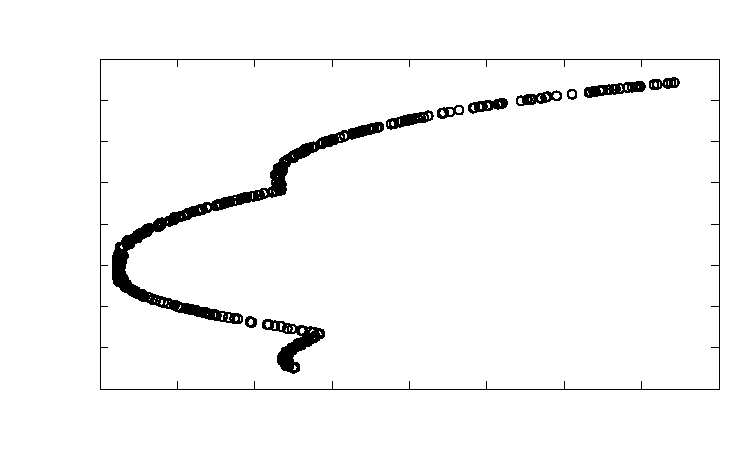
\includegraphics{GRAPH_color_graph2}}%
    \gplfronttext
  \end{picture}%
\endgroup

						}\endgroup
				\caption{B\label{fig:col2}}
			\end{minipage}
			\begin{minipage}[c]{0.5\linewidth}
				\centering
					\begingroup\endlinechar=-1
						\resizebox{\textwidth}{!}{%
							% GNUPLOT: LaTeX picture with Postscript
\begingroup
  \makeatletter
  \providecommand\color[2][]{%
    \GenericError{(gnuplot) \space\space\space\@spaces}{%
      Package color not loaded in conjunction with
      terminal option `colourtext'%
    }{See the gnuplot documentation for explanation.%
    }{Either use 'blacktext' in gnuplot or load the package
      color.sty in LaTeX.}%
    \renewcommand\color[2][]{}%
  }%
  \providecommand\includegraphics[2][]{%
    \GenericError{(gnuplot) \space\space\space\@spaces}{%
      Package graphicx or graphics not loaded%
    }{See the gnuplot documentation for explanation.%
    }{The gnuplot epslatex terminal needs graphicx.sty or graphics.sty.}%
    \renewcommand\includegraphics[2][]{}%
  }%
  \providecommand\rotatebox[2]{#2}%
  \@ifundefined{ifGPcolor}{%
    \newif\ifGPcolor
    \GPcolortrue
  }{}%
  \@ifundefined{ifGPblacktext}{%
    \newif\ifGPblacktext
    \GPblacktexttrue
  }{}%
  % define a \g@addto@macro without @ in the name:
  \let\gplgaddtomacro\g@addto@macro
  % define empty templates for all commands taking text:
  \gdef\gplbacktext{}%
  \gdef\gplfronttext{}%
  \makeatother
  \ifGPblacktext
    % no textcolor at all
    \def\colorrgb#1{}%
    \def\colorgray#1{}%
  \else
    % gray or color?
    \ifGPcolor
      \def\colorrgb#1{\color[rgb]{#1}}%
      \def\colorgray#1{\color[gray]{#1}}%
      \expandafter\def\csname LTw\endcsname{\color{white}}%
      \expandafter\def\csname LTb\endcsname{\color{black}}%
      \expandafter\def\csname LTa\endcsname{\color{black}}%
      \expandafter\def\csname LT0\endcsname{\color[rgb]{1,0,0}}%
      \expandafter\def\csname LT1\endcsname{\color[rgb]{0,1,0}}%
      \expandafter\def\csname LT2\endcsname{\color[rgb]{0,0,1}}%
      \expandafter\def\csname LT3\endcsname{\color[rgb]{1,0,1}}%
      \expandafter\def\csname LT4\endcsname{\color[rgb]{0,1,1}}%
      \expandafter\def\csname LT5\endcsname{\color[rgb]{1,1,0}}%
      \expandafter\def\csname LT6\endcsname{\color[rgb]{0,0,0}}%
      \expandafter\def\csname LT7\endcsname{\color[rgb]{1,0.3,0}}%
      \expandafter\def\csname LT8\endcsname{\color[rgb]{0.5,0.5,0.5}}%
    \else
      % gray
      \def\colorrgb#1{\color{black}}%
      \def\colorgray#1{\color[gray]{#1}}%
      \expandafter\def\csname LTw\endcsname{\color{white}}%
      \expandafter\def\csname LTb\endcsname{\color{black}}%
      \expandafter\def\csname LTa\endcsname{\color{black}}%
      \expandafter\def\csname LT0\endcsname{\color{black}}%
      \expandafter\def\csname LT1\endcsname{\color{black}}%
      \expandafter\def\csname LT2\endcsname{\color{black}}%
      \expandafter\def\csname LT3\endcsname{\color{black}}%
      \expandafter\def\csname LT4\endcsname{\color{black}}%
      \expandafter\def\csname LT5\endcsname{\color{black}}%
      \expandafter\def\csname LT6\endcsname{\color{black}}%
      \expandafter\def\csname LT7\endcsname{\color{black}}%
      \expandafter\def\csname LT8\endcsname{\color{black}}%
    \fi
  \fi
  \setlength{\unitlength}{0.0500bp}%
  \begin{picture}(7200.00,4320.00)%
    \gplgaddtomacro\gplbacktext{%
      \put(849,595){\makebox(0,0)[r]{\strut{} 11}}%
      \put(849,912){\makebox(0,0)[r]{\strut{} 11.5}}%
      \put(849,1228){\makebox(0,0)[r]{\strut{} 12}}%
      \put(849,1545){\makebox(0,0)[r]{\strut{} 12.5}}%
      \put(849,1861){\makebox(0,0)[r]{\strut{} 13}}%
      \put(849,2178){\makebox(0,0)[r]{\strut{} 13.5}}%
      \put(849,2495){\makebox(0,0)[r]{\strut{} 14}}%
      \put(849,2811){\makebox(0,0)[r]{\strut{} 14.5}}%
      \put(849,3128){\makebox(0,0)[r]{\strut{} 15}}%
      \put(849,3444){\makebox(0,0)[r]{\strut{} 15.5}}%
      \put(849,3761){\makebox(0,0)[r]{\strut{} 16}}%
      \put(951,409){\makebox(0,0){\strut{} 1.5}}%
      \put(1694,409){\makebox(0,0){\strut{} 2}}%
      \put(2437,409){\makebox(0,0){\strut{} 2.5}}%
      \put(3179,409){\makebox(0,0){\strut{} 3}}%
      \put(3922,409){\makebox(0,0){\strut{} 3.5}}%
      \put(4665,409){\makebox(0,0){\strut{} 4}}%
      \put(5408,409){\makebox(0,0){\strut{} 4.5}}%
      \put(6150,409){\makebox(0,0){\strut{} 5}}%
      \put(6893,409){\makebox(0,0){\strut{} 5.5}}%
      \csname LTb\endcsname%
      \put(144,2178){\rotatebox{-270}{\makebox(0,0){\strut{}Y-J}}}%
      \csname LTb\endcsname%
      \put(3922,130){\makebox(0,0){\strut{}J-H}}%
      \put(3922,4040){\makebox(0,0){\strut{}Redshift 8.5--10.1}}%
    }%
    \gplgaddtomacro\gplfronttext{%
    }%
    \gplbacktext
    \put(0,0){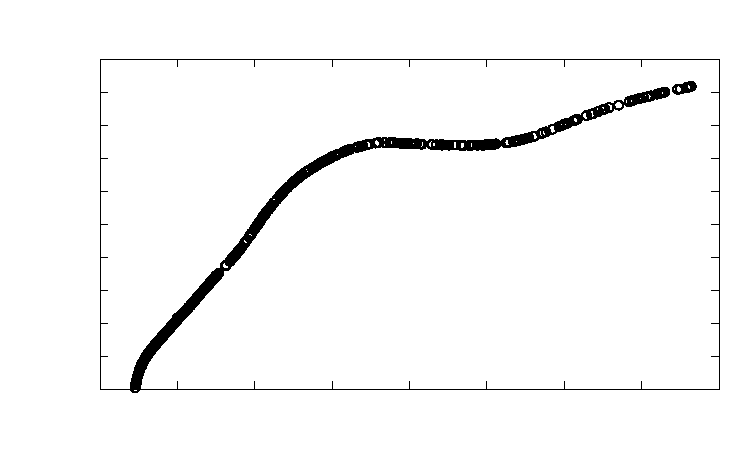
\includegraphics{GRAPH_color_graph3}}%
    \gplfronttext
  \end{picture}%
\endgroup

						}\endgroup
				\caption{C\label{fig:col3}}
			\end{minipage}
			\begin{minipage}[c]{0.5\linewidth}
				\centering
					\begingroup\endlinechar=-1
						\resizebox{\textwidth}{!}{%
							% GNUPLOT: LaTeX picture with Postscript
\begingroup
  \makeatletter
  \providecommand\color[2][]{%
    \GenericError{(gnuplot) \space\space\space\@spaces}{%
      Package color not loaded in conjunction with
      terminal option `colourtext'%
    }{See the gnuplot documentation for explanation.%
    }{Either use 'blacktext' in gnuplot or load the package
      color.sty in LaTeX.}%
    \renewcommand\color[2][]{}%
  }%
  \providecommand\includegraphics[2][]{%
    \GenericError{(gnuplot) \space\space\space\@spaces}{%
      Package graphicx or graphics not loaded%
    }{See the gnuplot documentation for explanation.%
    }{The gnuplot epslatex terminal needs graphicx.sty or graphics.sty.}%
    \renewcommand\includegraphics[2][]{}%
  }%
  \providecommand\rotatebox[2]{#2}%
  \@ifundefined{ifGPcolor}{%
    \newif\ifGPcolor
    \GPcolortrue
  }{}%
  \@ifundefined{ifGPblacktext}{%
    \newif\ifGPblacktext
    \GPblacktexttrue
  }{}%
  % define a \g@addto@macro without @ in the name:
  \let\gplgaddtomacro\g@addto@macro
  % define empty templates for all commands taking text:
  \gdef\gplbacktext{}%
  \gdef\gplfronttext{}%
  \makeatother
  \ifGPblacktext
    % no textcolor at all
    \def\colorrgb#1{}%
    \def\colorgray#1{}%
  \else
    % gray or color?
    \ifGPcolor
      \def\colorrgb#1{\color[rgb]{#1}}%
      \def\colorgray#1{\color[gray]{#1}}%
      \expandafter\def\csname LTw\endcsname{\color{white}}%
      \expandafter\def\csname LTb\endcsname{\color{black}}%
      \expandafter\def\csname LTa\endcsname{\color{black}}%
      \expandafter\def\csname LT0\endcsname{\color[rgb]{1,0,0}}%
      \expandafter\def\csname LT1\endcsname{\color[rgb]{0,1,0}}%
      \expandafter\def\csname LT2\endcsname{\color[rgb]{0,0,1}}%
      \expandafter\def\csname LT3\endcsname{\color[rgb]{1,0,1}}%
      \expandafter\def\csname LT4\endcsname{\color[rgb]{0,1,1}}%
      \expandafter\def\csname LT5\endcsname{\color[rgb]{1,1,0}}%
      \expandafter\def\csname LT6\endcsname{\color[rgb]{0,0,0}}%
      \expandafter\def\csname LT7\endcsname{\color[rgb]{1,0.3,0}}%
      \expandafter\def\csname LT8\endcsname{\color[rgb]{0.5,0.5,0.5}}%
    \else
      % gray
      \def\colorrgb#1{\color{black}}%
      \def\colorgray#1{\color[gray]{#1}}%
      \expandafter\def\csname LTw\endcsname{\color{white}}%
      \expandafter\def\csname LTb\endcsname{\color{black}}%
      \expandafter\def\csname LTa\endcsname{\color{black}}%
      \expandafter\def\csname LT0\endcsname{\color{black}}%
      \expandafter\def\csname LT1\endcsname{\color{black}}%
      \expandafter\def\csname LT2\endcsname{\color{black}}%
      \expandafter\def\csname LT3\endcsname{\color{black}}%
      \expandafter\def\csname LT4\endcsname{\color{black}}%
      \expandafter\def\csname LT5\endcsname{\color{black}}%
      \expandafter\def\csname LT6\endcsname{\color{black}}%
      \expandafter\def\csname LT7\endcsname{\color{black}}%
      \expandafter\def\csname LT8\endcsname{\color{black}}%
    \fi
  \fi
  \setlength{\unitlength}{0.0500bp}%
  \begin{picture}(7200.00,4320.00)%
    \gplgaddtomacro\gplbacktext{%
      \put(645,595){\makebox(0,0)[r]{\strut{} 10}}%
      \put(645,947){\makebox(0,0)[r]{\strut{} 15}}%
      \put(645,1299){\makebox(0,0)[r]{\strut{} 20}}%
      \put(645,1650){\makebox(0,0)[r]{\strut{} 25}}%
      \put(645,2002){\makebox(0,0)[r]{\strut{} 30}}%
      \put(645,2354){\makebox(0,0)[r]{\strut{} 35}}%
      \put(645,2706){\makebox(0,0)[r]{\strut{} 40}}%
      \put(645,3057){\makebox(0,0)[r]{\strut{} 45}}%
      \put(645,3409){\makebox(0,0)[r]{\strut{} 50}}%
      \put(645,3761){\makebox(0,0)[r]{\strut{} 55}}%
      \put(747,409){\makebox(0,0){\strut{} 0}}%
      \put(1515,409){\makebox(0,0){\strut{} 2}}%
      \put(2284,409){\makebox(0,0){\strut{} 4}}%
      \put(3052,409){\makebox(0,0){\strut{} 6}}%
      \put(3820,409){\makebox(0,0){\strut{} 8}}%
      \put(4588,409){\makebox(0,0){\strut{} 10}}%
      \put(5357,409){\makebox(0,0){\strut{} 12}}%
      \put(6125,409){\makebox(0,0){\strut{} 14}}%
      \put(6893,409){\makebox(0,0){\strut{} 16}}%
      \csname LTb\endcsname%
      \put(144,2178){\rotatebox{-270}{\makebox(0,0){\strut{}f150w-f200w}}}%
      \csname LTb\endcsname%
      \put(3820,130){\makebox(0,0){\strut{}f115w-f150w}}%
      \put(3820,4040){\makebox(0,0){\strut{}Redshift 10--14}}%
    }%
    \gplgaddtomacro\gplfronttext{%
    }%
    \gplbacktext
    \put(0,0){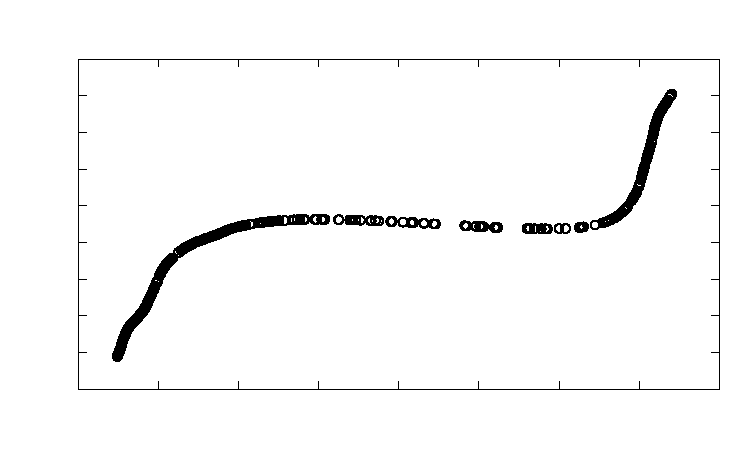
\includegraphics{GRAPH_color_graph4}}%
    \gplfronttext
  \end{picture}%
\endgroup

						}\endgroup
				\caption{D\label{fig:col4}}
			\end{minipage}
			\caption{Graphs showing the colour-colour regions for \\
			(A) z=6-7.5. The colour window was defined as $f070w-f090w{\ge}3.257$ and $f090w-f115w{\le}8.242$,\\
			(B) z=7.5-8.5. The colour window was defined as $f090w-f115w{\ge}8.251$ and $f115w-f150w{\le}2.869$, \\
			(C) z=8.54-10.1. The colour window was defined as $Y-J{\ge}11.019$ and $J-H{\le}5.298$, \\
			(D) z=10-14. The colour window was defined as $f115w-f150w{\ge}14.439$ and $f150w-f200w{\le}14.815$}
		\end{figure}
	%subsection Results_for_Colour (end)

	\subsection{Interpretation of Colour Results}
	\label{sub:Interp_Colour}
		Constraining a colour window for observations turned out to be a challenging task. The filter 275w on James Webb didn't work properly in Hyperz; some magnitudes came out as 99.0 which is the default answer if there was an error; other magnitudes were above 100. As the source of this error could not be found, the range of redshift 14 to 15 was taken from the colour window results. The colour window results  shown in Figures~\ref{fig:col1},~\ref{fig:col2},~\ref{fig:col3} and~\ref{fig:col4} are much higher than expected results such as the colour windows in \cite{lorenzoni2013constraining}. Something must be wrong with the technique that was used to find the colours, however in defense of the results, the assumptions made as described in the sections above were reasonably fair for the timescale of the project. It's hard to say if there is one set of inputs or parameters that were the main source of error.  The shape of the distribtution of the galaxies is odd but seems to follow a pattern for each redshift range, which remains unexplained. The other peculiar characteristic of the diagrams is that all the galaxies appear on a mainly continous line, as opposed to being distributed in a certain area. Having done some basic tests, the cause of this appears to be due to setting the age of the galaxies at the same redshift to be the same; as soon as the age was randomised to some time between the formation redshift and the observed redshift, the galaxies were more spread out. However these galaxies appeared `inside' the colour window, so this doesn't appear to have affected the determination of the colour windows.
	%section Interpetation_of_colour_results (end)
%section Photometry_and_colour (end)

    % %!TEX root = mainfile.tex

\section{Contaminants} % (fold)
\label{sec:contaminants}
    \subsection{Low Mass Stars} % (fold)
    \label{sub:low_mass_stars}
        These can easily be identified due to the high resolution imaging provided by \ldots. The Point-spread function (PSF) obtained will allow us to determine which sources are point-like and which are extended. We should be able to avoid significant contamination by removing any point-like sources from the results as all galaxies should have a great enough diameter.
    % subsection low_mass_stars (end)

    \subsection{Spurious Sources} % (fold)
    \label{sub:spurious_sources}
        By stipulating that we will be requiring detections in two bands the influence of spurious sources will be negligible. Finding detections in 2 bands at reasonable confidence interval (?3sig?) is very improbable. By inspecting the negative with the same requirements for detection we are able to identify any such sources easily\cite{Bouwens2011}.
    % subsection spurious_sources (end)

    \subsection{Supernovae and other transient sources} % (fold)
    \label{sub:supernovae_and_other_transient_sources}
        Events such as Supernovae happen incredibly quickly releasing a vast amount of energy, as seen in figure~\ref{fig:SNe_1987a}. These events can spoil images due to their short duration by introducing new data in only a portion of the sample. These effects are usually only considered when taking exposures years apart or when combining multiple sources over a long time scale. Such events are very unlikely to contaminate our results as we propose to take our images close in time.
        \begin{figure}[!htb]
            \centering
            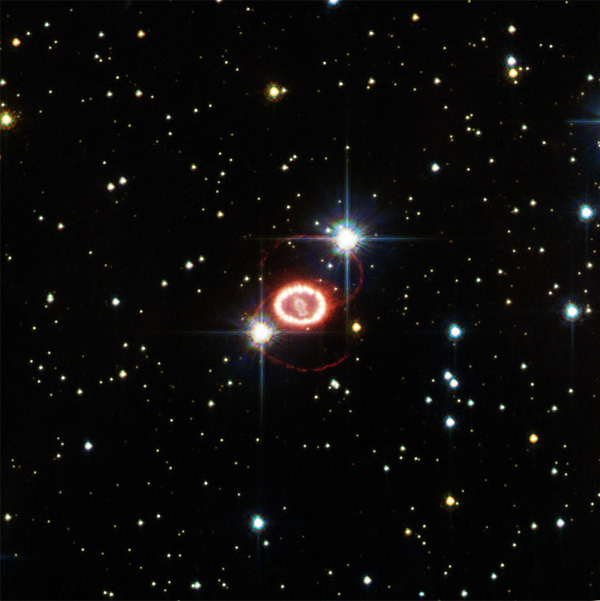
\includegraphics[width=0.6\textwidth]{../Images/SNe_1987a.jpg}
            \caption{The shock wave from Supernova 1987a imaged by HST in 2006.\label{fig:SNe_1987a}}
        \end{figure}
    % subsection supernovae_and_other_transient_sources (end)

    \subsection{Lower Redshift Sources and photometric scattering} % (fold)
    \label{sub:lower_redshift_sources_and_photometric_scattering}
        This category is likely to provide the greatest source of contamination for the surveyed area. It will do so increasingly at high redshifts where its affect on the faintest magnitudes is most greatly felt. Its affect is most influential with a small S/N ratio for the observations, by fixing this at a level of S/N = \ldots we can be confident that the contamination will be low. Detecting a source in another band such as b435, v606, i775 for YJH photometry would class it as a contaminant and then should be removed from sample.
    % subsection lower_redshift_sources_and_photometric_scattering (end)

% section contaminants (end)

    % \clearpage
    \section{The Evolution of the Neutral Hydrogen Fraction} % (fold)
\label{sec:the_evolution_of_the_neutral_hydrogen_fraction}
(Rahim)

	In order to place redshift limits on the epoch of reionization, the neutral hydrogen fraction will be calculated from the data procured. The optical depth will first be calculated using equation~(\ref{eq:optical_depth}) where the measured continuum flux can be compared to flux from an identical part of the spectrum of a lower redshift galaxy where the Gunn-Peterson trough is not visible. This can be done as the emitted spectra of Lyman break galaxies are very similar to that of much closer galaxies.

	The neutral hydrogen fraction can then be calculated via equation~(\ref{eq:gunn-peterson_tau}) and plotted as a function of redshift. Thus, when the neutral hydrogen fraction falls, a limit can be placed at a particular redshift for the end of the epoch of reionization. Figure~\ref{fig:Evolution_Xh1} shows an example of this where numerous methods are used to plot the evolution of the neutral hydrogen fraction\cite{Fanetal}.
	\begin{figure}[htbp]
		\centering
		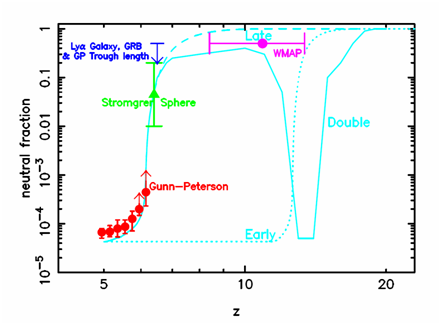
\includegraphics[width=0.5\textwidth]{../Images/Evolution_Xh1.png}
		\caption{The volume averaged fraction of neutral hydrogen in the IGM versus redshift. The fiducial model of late reionization is represented by the dashed line, an idealised model including double reionization is represented by the solid line and an early reionization model is represented by the dotted line.}\label{fig:Evolution_Xh1}
	\end{figure}

	With an initially large neutral hydrogen fraction, the radiation from early galaxies will start to ionise the neutral hydrogen causing the fraction to decrease indicating the start of the EoR. Towards the end of the EoR, at a certain redshift the spectra from galaxies will not show the Gunn-Peterson trough indicating a much lower fraction of neutral hydrogen. The redshift limit will therefore be the redshift at which production of the Gunn- Peterson trough ceases. Mapping the neutral hydrogen fraction should therefore place some rough limits on the start and end of the EoR.

	\subsection{Advantages and Disadvantages} % (fold)
	\label{sub:advantages_disadvantages}
		The main advantage of mapping the evolution of the neutral hydrogen fraction is that this can be done in conjunction with the dropout technique using the flux measured in that part of the observing strategy. However, a possible limitation of using the Gunn-Peterson absorption is that only a very small fraction of neutral hydrogen is required to produce complete Gunn-Peterson absorption. This means that the use of the Gunn-Peterson optical depth is more accurate towards the end of reionization where the IGM is already mostly ionised and the neutral hydrogen fraction is small. During the early part of reionization, it would be difficult to accurately measure the neutral hydrogen fraction as only a little is required to produce the Gunn-Peterson trough. However the redshift of the earliest galaxies in the universe will give the best idea of the redshift at which the EoR started as these galaxies contributed the first ionising radiation.
	% subsection advantages_disadvantages (end)
% section the_evolution_of_the_neutral_hydrogen_fraction (end)

    %!TEX root = mainfile.tex

\section{Photometry Exposure Times} % (fold)
\label{sec:exposure_times}
(Rahim, except~\ref{sub:full_width_at_half_maximum} Dorothy and Mike)

	The main aim of this project is to produce an observing strategy to view some of the earliest galaxies in the universe and map the epoch of reionization during which they were produced. An important aspect of this is therefore the viewing of the galaxies themselves and the time it will take to do so. The time required to view these galaxies depends not only on the telescope being used, but also the devices used. A charged coupled device (CCD) will be used to measure the light from these sources and so to calculate the times required to view these galaxies, these must be understood in more detail. The telescope or telescopes used during the observation of these galaxies will have different properties which will affect the time required to view the source. Some of these are discussed below.

	\subsection{Telescope Properties} % (fold)
	\label{sub:telescope_properties}
		\subsubsection{Mirror Reflectivity} % (fold)
		\label{ssub:mirror_reflectivity}
			One such factor that will increase the time required to view a source is the reflectivity of the mirrors used on the telescope. The mirror reflectivity, given as a percentage, is the amount of light reflected by the mirror. Some of the light is absorbed by the miror producing heat as it is not 100\% efficient meaning not all photons striking the mirror reach the the next mirror or the CCD. The reflectivity differs depending on the material used on the surface of the mirrors. Various optical coatings are produced and used depending on the wavelengths being observed, for example, the James Webb Space Telescope uses a gold coating which is particularly useful in the infrared region and is also very durable due to the inert nature of gold. The reflectivity of this gold coated mirror is in the region of 98\%--99\%\cite{Quantum_Coatings_Incorporated}. Other coatings regularly used include aluminium, which has a reflectivity in the region of 80\%--90\% and is utilised in the UV and IR range, as well as silver, which has a reflectivity in the range of 95\%--99\% and is utilised in the visible and IR range.
		% subsubsection mirror_reflectivity (end)

		\subsubsection{Telescope Throughput} % (fold)
		\label{ssub:telescope_throughput}
			The definition of throughput is the ratio of the flux detected by a particular instrument in a given filter and the incoming flux measured over an area equal to the area of the telescope primary mirror\cite{WIRCam_Throughput}. The throughput is therefore the percentage of photons striking the primary mirror that reach the CCD and are recorded. This contributes to the time required to observe a source as not all the photons striking the primary mirror, originating from the source, will reach the CCD. As the number of photons reaching the CCD is fewer, a larger portion of time is required to obtain the sought after signal-to-noise ratio and so the overall observation lasts a longer period of time.
		% subsubsection telescope_throughput (end)

		\subsubsection{Filters} % (fold)
		\label{ssub:filters}
			An astronomical filter is used on telescopes to remove light of unwanted wavelengths above and below a certain bandpass where a bandpass is a range of wavelengths that can pass through the filter. The width of this bandpass is commonly known as the bandwidth and is often used in astronomical calculations. The filter used will contain the specific wavelength being observed within the bandpass and reduce flux from other parts of the spectrum. A narrower filter will therefore ensure less background flux is observed reducing the error on the number of photons arriving from the source.

			A filter is usually denoted with the central wavelength and width of the filter. For example, one particular filter used on the James Webb Space Telescope is named F160N, denoting a central wavelength of \SI{1.6}{\micro\metre} and a narrow bandwidth. The bandwidth can then be found as it will be specific to the filter.

			The filter used is dependent on the redshifted wavelength of light from the source being observed. The wavelength of the redshifted light will be matched to a filter with the closest central wavelength to this wavelength. The bandpass of the telescope is the range of wavelengths that can pass through the filter and be measured as flux and so matching the redshifted wavelength to a filter with a similar central wavelength will allow the most flux from the source to be measured.
		% subsubsection filters (end)

		\subsubsection{Field of View} % (fold)
		\label{ssub:field_of_view}
			The field of view is specific to each telescope and gives the area of sky that is subtended by the CCD. This therefore depends on the CCD and the angle of sky subtended by each pixel. From this, the total area of sky imaged on the CCD can be determined. This is an important factor to take into account during the final observing strategy as, although a particular telescope may be quicker in finding a source, a larger field of view will mean more galaxies can be viewed. This therefore means a compromise must be produced to develop the optimum observing strategy.
		% subsubsection field_of_view (end)
	% subsection telescope_properties (end)

	\subsection{Charged Coupled Devices} % (fold)
	\label{sub:charged_coupled_devices}
		A charged coupled device or CCD is currently the detector of choice in astronomy and is used to produce images using incoming photons. A CCD works over a broad range of wavelengths and generally has high quantum efficiency within this range. They can vary in size from \SI{1.3}{\milli\metre} to up to \SI{70}{\milli\metre} across the diagonal. A larger size means more photosites and usually better image quality however the price of a CCD unfortunately rises exponentially with size ranging from \$60 to \$4000. They are still regarded as the best detectors available to astronomers and so are widely used in astronomical observations.

		CCDs consist of an array of metal-oxide semiconductor (MOS) capacitors, known as photo-detector junctions or photosites, formed on a silicon substrate. One pixel in the CCD can contain between one and a few of these capacitors. Each photosite contains a charge isolated from other photosites by a voltage applied through conductive channels on the surface of the silicon\cite{Diffraction_Limited_Imaging_Saha}. The MOS capacitor is structured with a metal electrode applied on top of a silicon substrate usually separated by a thin layer of insulation. At the beginning of each exposure, the electrodes are positively charged repelling holes in the substrate forming a depletion region which is an electrostatic potential well. Photons entering the substrate free electrons via the photoelectric effect and these are then attracted to the positively charged electrode and so are collected in the depletion region. The holes generated are repelled away from the depletion region and are lost in the substrate. The electrons generated can then be collected in the pixel and are counted to reproduce the pattern of the incident light producing an image.

		The photosites on a CCD are arranged in columns and lines convenient for the readout procedure. The array contains a special row of photosites on the bottom line known as the serial register. Upon completion of the exposure, the electrons in the columns of the array are clocked down one line with the bottom line entering the serial register. The serial register is then clocked into a charge detection node moving one pixel at a time. The electrons move along the row towards the charge detection node and upon completion of clocking each row, the next row up will drop into the serial register and be clocked in an identical fashion\cite{Astronomical_Image_Processing}. During this readout procedure, a shutter must be applied to prevent light generating further electrons. The readout time of a CCD can vary from a fraction of a second to around ten seconds.

		The CCD does however have numerous errors known as noise, which contribute to the integration time required to view the distant galaxies being examined in this project and so must be taken into account. The conversion of light to pixel values in a CCD leads to an inevitable noise being introduced into the image. This noise is the unwanted variations in pixel values and causes the image produced to differ from the one being observed. The noise incurred will make it more difficult to distinguish the source being observed hence increasing the integration time. For an electrical measuring system such as a CCD, a signal to noise ratio characterises the quality of the measurement taken where the signal to noise ratio ($\frac{S}{N}$) is the ratio of signal from the source being observed and signal produced by background radiation and other sources of noise. The main sources of noise for a CCD are the Poisson error, dark current, sky background and read noise, which are all described below.


		\subsubsection{Poisson Error} % (fold)
		\label{ssub:poisson_error}
			The Poisson error ($\sigma_\text{Poisson}$) or photon counting error is due to variations in the incoming flux of a source. As the photons from the source arrive randomly, the actual number arriving at a certain time or in a small time interval may differ from the average and so the error is on the detection of these photons. The Poisson error can be calculated quite simply as the error is the square root of the number of counts. This is shown in equation~(\ref{eq:poisson_error_sqrt_Ft}) where $F$ is the incoming flux and t is the exposure time.
			\begin{align}
				\sigma_\text{Poisson} = \sqrt{Ft} \label{eq:poisson_error_sqrt_Ft}
			\end{align}
		% subsubsection poisson_error (end)

		\subsubsection{Dark Current} % (fold)
		\label{ssub:dark_current}
			Dark current ($\sigma_\text{Dark}$), also known as thermal current, is due to the random generation of electrons and holes within the substrate of the MOS capacitor. Atoms in the silicon substrate of the CCD used are thermally excited and thus electrons are freed. These are then counted along with the electrons freed by photons from the object being observed. This occurs even when the CCD is not exposed to light, hence there is a steady creation of electrons, and this is called the dark or thermal current. As this is caused by thermal excitation, it strongly depends on the temperature at which the device is operating. At any given temperature, the rate at which electrons are freed is constant, however for every rise in temperature of 6 degrees Celsius, the dark current produced approximately doubles\cite{Astronomical_Image_Processing}. This relationship is shown in Figure~\ref{fig:dark_current_vs_temp}\cite{Southern_Observatory_throughput}.
			\begin{figure}[htbp]
				\centering
				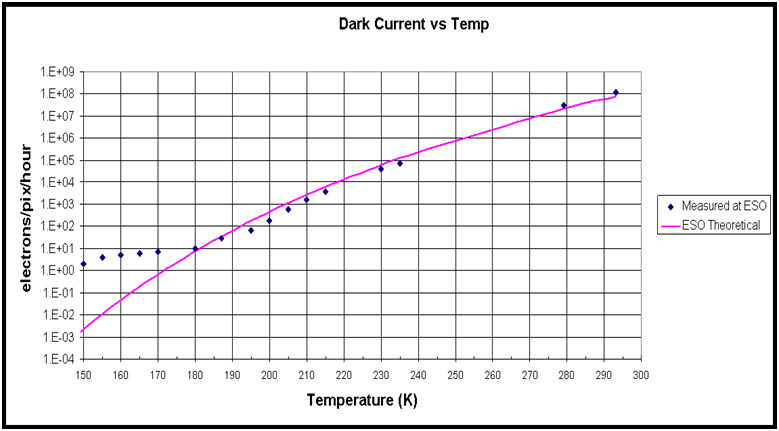
\includegraphics[width=0.6\textwidth]{../Images/Dark.png}
				\caption{A graph showing the relationship between dark current and temperature.\label{fig:dark_current_vs_temp}}
			\end{figure}

			Figure~\ref{fig:dark_current_vs_temp} shows that relationship between temperature and dark current for a custom designed CCD provided to the European Southern Observatory and shows clearly the increase in dark current at higher temperatures. CCD's are therefore cooled, often with the use of liquid nitrogen, to minimise this effect. The dark current itself is a relatively small electric current that flows through numerous photosensitive devices, and is one of the main sources of noise for a CCD. The dark noise contributed to the total noise can be calculated using the formula below where $D$ is the dark current in electrons per second per pixel, $t$ is the exposure time in seconds and N$_\text{pix}$ is the number of pixels in the CCD aperture.
			\begin{align}
				\sigma_\text{Dark} = \sqrt{DN_\text{pix}t}
			\end{align}
		% subsubsection dark_current (end)

		\subsubsection{Sky Background} % (fold)
		\label{ssub:sky_background}
			The sky background is the incoming light from the sky measured on the telescope that is not from the source being observed. The amount of sky background can vary at different wavelengths and is mainly due to light diffusion by the atmosphere. There are numerous sources that contribute towards the sky background such as airglow, zodiacal light and thermal radiation.

			Airglow is the atmospheric emission of photons at wavelengths from the near-UV to the near-IR range due to chemical reactions in the upper atmosphere\cite[p.~9]{An_atmospheric_radiation_model_for_Cerro_Paranal}. These chemical reactions lead to photon emissions due to the decay of electrons from an excited state in one of the reaction products. One such example is the emission in the near infrared region by OH radicals created from a reaction between ozone and hydrogen in the upper atmosphere\cite[p.~1]{MNRMNR11383}. Other processes contributing to airglow are the recombination of ions originally ionised by the sun, and the luminescence of cosmic rays striking the upper atmosphere. Airglow therefore produces a faint glow and can be seen in Figure~\ref{fig:air_glow_in_upper_atmosphere}.
			% \begin{figure}[htbp]
			% 	\centering
			% 	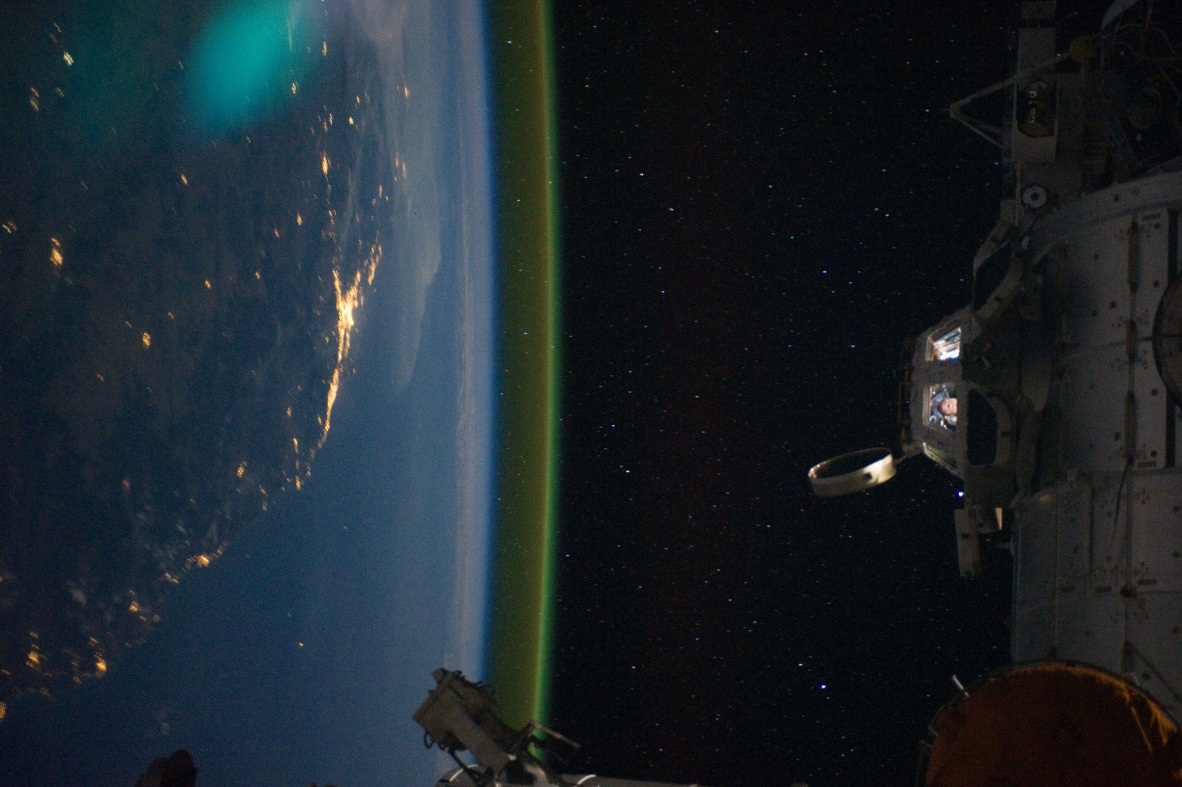
\includegraphics[width=0.7\textwidth]{../Images/airglow_in_upper_atmosphere.jpeg}
			% 	\caption{Airglow in the upper atmosphere as observed from the International Space Station\cite{ISS028_E_050185}}\label{fig:air_glow_in_upper_atmosphere}
			% \end{figure}
			% \begin{figure}[htbp]
			% 	\centering
			% 	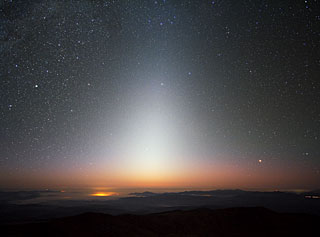
\includegraphics[width=0.7\textwidth]{../Images/zodiacal_light.jpeg}
			% 	\caption{An image of zodiacal light above the earth}\label{fig:air_glow_in_upper_atmosphere}
			% \end{figure}
			\begin{figure}[htbp]
				\begin{minipage}[c]{0.5\linewidth}
					\centering
					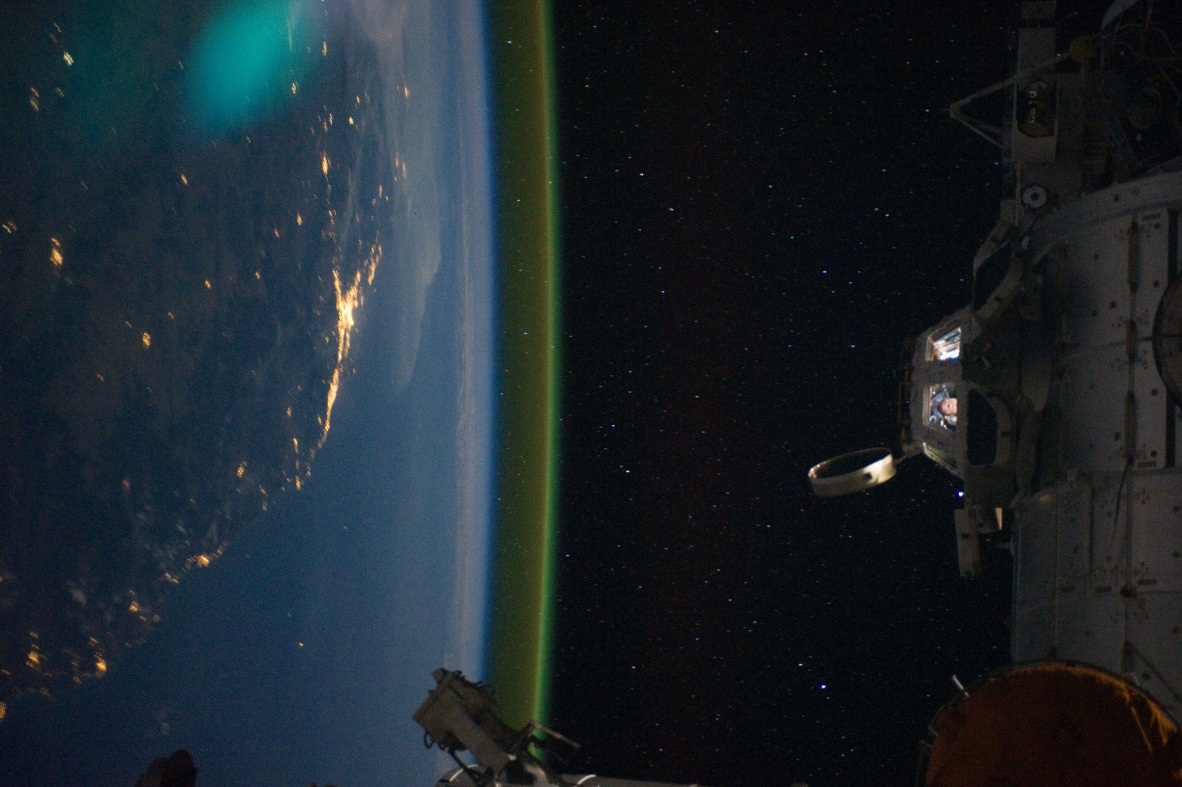
\includegraphics[height=4.5cm]{../Images/airglow_in_upper_atmosphere.jpeg}
				\end{minipage}
				\begin{minipage}[c]{0.5\linewidth}
					\centering
					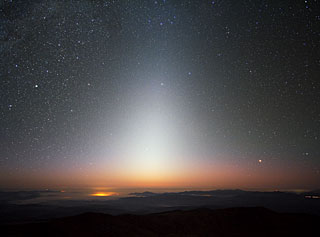
\includegraphics[height=4.5cm]{../Images/zodiacal_light.jpeg}
				\end{minipage}
				\caption{Left: Airglow in the upper atmosphere as observed from the International Space Station\cite{ISS028_E_050185}. Right: An image of zodiacal light above the earth}\label{fig:air_glow_in_upper_atmosphere}
			\end{figure}

			Another of the contributors to the sky background is zodiacal light which is the scattering of sunlight off interplanetary dust\cite[p.~5--6]{MNRMNR21602}. This can be seen in Figure~\ref{fig:air_glow_in_upper_atmosphere} below. This causes a faint white glow that can be best seen before sunrise or after sunset but is generally so faint it cannot be seen over moonlight or light pollution. The dust in the solar system forms a thick lens shape cloud known as the interplanetary dust cloud or zodiacal cloud and it is off this cloud that light from the Sun is scattered. Zodiacal light is mainly seen in the ecliptic plane, the plane of the solar system, as most of the dust making up this cloud is located in this plane. Another similar effect to this is the gegenschein, or counter shine, which is a faint glow in the antisolar direction\cite{Observational_Studies_of_Interplanetary_Dust}. At this point, the zodiacal light is enhanced by backscattering off interplanetary dust producing a small brightening in this part of the sky.

			Background from zodiacal light can however be greatly reduced by observing outside of the ecliptic plane as this is where the flux of photons due to zodiacal light is weakest. This can be seen in Figure~\ref{fig:air_glow_in_upper_atmosphere_graph} below which shows the flux of photons as a function of angle to the ecliptic plane.
			\begin{figure}[htbp]
				\centering
				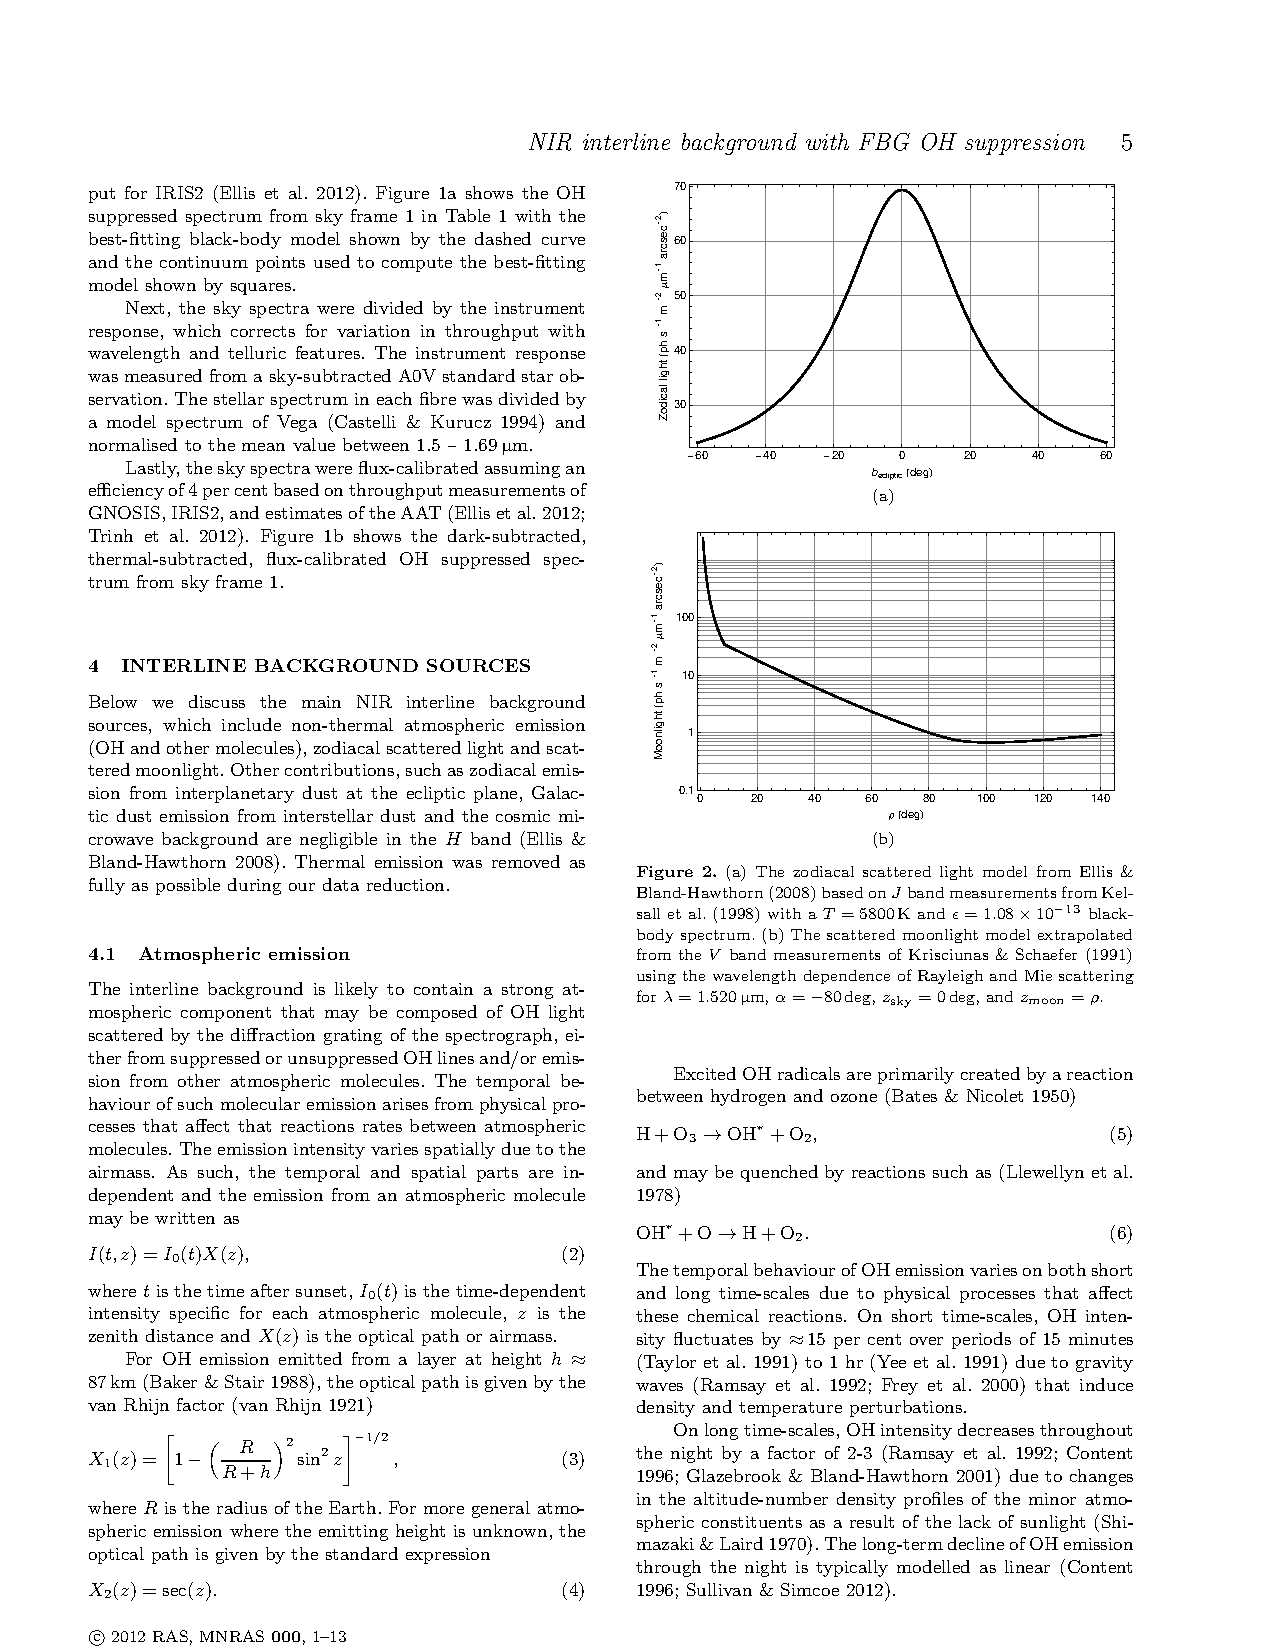
\includegraphics[trim = 110mm 198mm 25mm 30mm, clip, width=0.4\textwidth]{../Images/zodiacal_Light_graph.pdf}
				\caption[Zodiacal light vs angle]{The relationship between intensity of zodiacal light and the angle to the plane of the solar sytem}\label{fig:air_glow_in_upper_atmosphere_graph}
			\end{figure}

			The zodiacal light is strongest at a very small angle to the ecliptic plane but significantly decreases as the angle increases and so viewing well outside the ecliptic plane should considerably reduce background from zodiacal light\cite{Zodiacal_Light_over_La_Silla}.Thermal radiation in the atmosphere by greenhouse gases also contributes to the sky background and is due to the absorption and emission of radiation from the Sun into the atmosphere in the mid-IR region. In this case, observations in the mid- and far-IR region must be carried out from outside the atmosphere\cite{Extragalactic_Astronomy_and_Cosmology}. The sky background is therefore primarily an issue for ground based telescopes as they can incur a large background number of photons compared to the number of photons arriving from the source being observed.

			As space based telescopes are situated outside of the atmosphere, they avoid almost all of this background with their main source of background coming in the form of zodiacal light or thermal background due to radiation from the Sun. This can be calculated by first determining the number of photons from this thermal background before converting to a noise represented by the number of electrons excited in the CCD. The number of photons, $N\gamma$, can be calculated using the formula,
			\begin{align}
				N_\gamma &= \frac{2k^3 T^3 \epsilon}{h^3 c^2} {\left[ \e{-x}\left( x^2 + 2x + 2 \right) \right]}^{x_2}_{x_1},
			\end{align}
			where $x=\frac{h\nu}{kt}$, $\nu$ is frequency, $k$ is the Boltzmann constant, $t$ is temperature, $h$ is Planck's constant, $c$ is the speed of light and $\epsilon$ is the emissivity. $x_1$ is the bluer end of the filter, i.e.\ the shorter wavelength whilst $x_2$ is the redder end of the filter, i.e.\ the longer wavelength. The full derivation of this can be seen in appendix~\ref{app:derivation_of_thermal_background}. This can then be used to calculate the number of electrons per second per pixel ($N_e$) on the CCD contributing towards the background via the formula,
			\begin{align}
				N_e &= N_\gamma A\epsilon_{\text{th}}\Omega_{\text{pix}},
			\end{align}
			Where $A$ is the collecting area of the telescope, $\epsilon_{\text{th}}$ is the throughput of the filter used and $\Omega_{\text{pix}}$ is the solid angle subtended by each pixel in steradians. Completing this calculation for the Hubble Space telescope gives a value of $N_e$ of \SI{0.02}{\electron\per\second\per\pixel}. Whilst this is not the dominant source of background for the Hubble telescope, this may be used to calculate a rough estimate of the thermal background of other space based telescopes such as Euclid and JWST which are located at the second Lagrange point, well away from any atmospheric background.

			The total sky background is measured to be $B$ photons per second per pixel and the noise contributed can be calculated using the formula below where $t$ is the exposure time and $N_\text{pix}$ is the number of pixels in the CCD aperture.
			\begin{align}
				\sigma_\text{Sky} = \sqrt{BN_\text{pix}t}
			\end{align}
		% subsubsection sky_background (end)

		\subsubsection{Read Noise} % (fold)
		\label{ssub:read_noise}
			When the electrons accumulated by the CCD are being read or clocked off and converted to a voltage, a readout noise ($\sigma_\text{RN}$), a small, random variation generated by the CCD's charge detection node is added. This noise is expressed as a number of electrons per second per pixel and is a fundamental trait of CCD's. It will, unfortunately, occur in all CCD's, from ones used in simple webcams to those used on the Hubble Space Telescope\cite{Understanding_CCD_Read_Noise}. The read noise contributed to the total noise can be calculated using the formula below where $R$ is the read noise of the CCD in electrons and $N_\text{pix}$ is the number of pixels in the CCD aperture.
			\begin{align}
				\sigma_\text{RN} = R\sqrt{N_\text{pix}}
			\end{align}
		% subsubsection read_noise (end)
	% subsection charged_coupled_devices (end)

	\subsection{Signal-to-noise Ratio} % (fold)
	\label{ssub:signal_to_noise_ratio}
		The quality of a CCD image is quantified by a signal-to-noise ratio which can be established from the source signal and all noise contributions. The different types of noise discussed above, all contribute to a total noise ($\sigma$) in the received signal which can be calculated using equation~(\ref{eq:total_noise_in_recieved_signal}).
		\begin{align}
			\sigma^{2} = \sigma_{Poisson}^{2} + \sigma_{Dark}^{2} + \sigma_{Sky}^{2} + \sigma_{RN}^{2} \label{eq:total_noise_in_recieved_signal}
		\end{align}
		As the CCD is exposed to incoming light, both the background and the source signal build up. The background is randomly and evenly distributed and so also contributes to the peak of the signal which therefore sits as a peak or peaks above a layer of background and so can be distinguished. This can be seen on Figure~\ref{fig:signal_noise_accumulation} below where B is labelled in the region of background\cite{Signal_to_Noise_Ratio}.
		\begin{figure}[htbp]
			\centering
			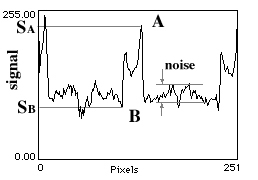
\includegraphics[width=0.4\textwidth]{../Images/SNR.png}
			\caption{The accumulation of signal, background and noise.\label{fig:signal_noise_accumulation}}
		\end{figure}

		The signal-to-noise ratio is therefore the total number of photons from the source reaching the CCD divided by the total noise for a given exposure time. As the exposure time increases, both signals, from source and background, cause an increase in counts establishing the signal more clearly. The signal-to-noise ratio is therefore also dependant on the exposure time although it is common for astronomers to decide on a signal-to-noise ratio to be obtained before calculating an exposure time.
		\begin{align}
			\frac{S}{N} = \frac{Ft}{\sigma} =\frac{Ft}{\sqrt{\sigma_\text{Poisson}^{2} + \sigma_\text{Dark}^{2} + \sigma_\text{Sky}^{2} + \sigma_{RN}^{2}}}
		\end{align}
		Either the signal-to-noise ratio or exposure time can then be calculated using the equation shown below commonly known as the CCD equation.
		\begin{align}
			\frac{S}{N} = \frac{Ft}{\sqrt{(F + BN_\text{pix} + DN_\text{pix})t + R{^2}N_\text{pix}}}
		\end{align}
		$F$ is the incident number of photons from the source per second, $t$ is the exposure time, $D$ is the dark current in electrons per second per pixel, $B$ is the sky background in photons per second per pixel and $R$ is the read noise in electrons. $N_\text{pix}$ is the number of pixels within the aperture area of the CCD and so is the number of pixels that are clocked to produce an image. This is dependent on the either the angular resolution of the telescope or the angular size of the object being observed depending on which is the limiting factor of the telescope and for photometry, can be calculated using equation~(\ref{eq:number_of_pixels_limiting}) below. The limiting factor becomes the FWHM in the equation and is discussed in Sections~\ref{sub:astronomical_seeing} and~\ref{sub:full_width_at_half_maximum} whilst $\theta_\text{pixel}$ is the angle subtended on the sky by one pixel. Observations on the James Webb Space Telescope will produce images with a signal-to-noise ratio of 10 indicating the current image quality desired.
		\begin{align}
			N_\text{pix} = \pi \left(\frac{4 \times \text{FWHM}}{\theta_\text{pixel}}\right)^2 \label{eq:number_of_pixels_limiting}
		\end{align}
	% subsubsection signal_to_noise_ratio (end)
% section exposure_times (end)

    %!TEX root = mainfile.tex

\subsection{Full Width at Half Maximum} % (fold)
\label{sub:full_width_at_half_maximum}
	To accurately calculate the FWHM of the galaxies it is essential to model them as extended bodies rather than point sources. To do this the angular size that a galaxy would subtend on the sky is calculated. The first requirement of this is to determine the size of an average galaxy. There have been limited detections of high redshift galaxies and even fewer have had their parameters defined using spectroscopy. Using values based on confirmed galaxies at redshifts of 6 and candidates at higher redshifts %[Ono_FWHM] [Bouwens_FWHM] [Oesc_FWHM] [Jiang_FWHM] the diameter of a galaxy is fixed at 1.5kpc for all redshifts.

	To avoid unnecessarily complex calculations a cosmological calculator\cite{Ned_Calc} is used to calculate the angular scale \si{\kilo\parsec\per ''} at the given redshifts, a plot of these values is shown in Figure~\ref{fig:redshift_vs_angular_size}.
	\begin{figure}[htbp]
		\centering
			\begingroup\endlinechar=-1
				\resizebox{0.6\textwidth}{!}{%
					% GNUPLOT: LaTeX picture with Postscript
\begingroup
  \makeatletter
  \providecommand\color[2][]{%
    \GenericError{(gnuplot) \space\space\space\@spaces}{%
      Package color not loaded in conjunction with
      terminal option `colourtext'%
    }{See the gnuplot documentation for explanation.%
    }{Either use 'blacktext' in gnuplot or load the package
      color.sty in LaTeX.}%
    \renewcommand\color[2][]{}%
  }%
  \providecommand\includegraphics[2][]{%
    \GenericError{(gnuplot) \space\space\space\@spaces}{%
      Package graphicx or graphics not loaded%
    }{See the gnuplot documentation for explanation.%
    }{The gnuplot epslatex terminal needs graphicx.sty or graphics.sty.}%
    \renewcommand\includegraphics[2][]{}%
  }%
  \providecommand\rotatebox[2]{#2}%
  \@ifundefined{ifGPcolor}{%
    \newif\ifGPcolor
    \GPcolortrue
  }{}%
  \@ifundefined{ifGPblacktext}{%
    \newif\ifGPblacktext
    \GPblacktexttrue
  }{}%
  % define a \g@addto@macro without @ in the name:
  \let\gplgaddtomacro\g@addto@macro
  % define empty templates for all commands taking text:
  \gdef\gplbacktext{}%
  \gdef\gplfronttext{}%
  \makeatother
  \ifGPblacktext
    % no textcolor at all
    \def\colorrgb#1{}%
    \def\colorgray#1{}%
  \else
    % gray or color?
    \ifGPcolor
      \def\colorrgb#1{\color[rgb]{#1}}%
      \def\colorgray#1{\color[gray]{#1}}%
      \expandafter\def\csname LTw\endcsname{\color{white}}%
      \expandafter\def\csname LTb\endcsname{\color{black}}%
      \expandafter\def\csname LTa\endcsname{\color{black}}%
      \expandafter\def\csname LT0\endcsname{\color[rgb]{1,0,0}}%
      \expandafter\def\csname LT1\endcsname{\color[rgb]{0,1,0}}%
      \expandafter\def\csname LT2\endcsname{\color[rgb]{0,0,1}}%
      \expandafter\def\csname LT3\endcsname{\color[rgb]{1,0,1}}%
      \expandafter\def\csname LT4\endcsname{\color[rgb]{0,1,1}}%
      \expandafter\def\csname LT5\endcsname{\color[rgb]{1,1,0}}%
      \expandafter\def\csname LT6\endcsname{\color[rgb]{0,0,0}}%
      \expandafter\def\csname LT7\endcsname{\color[rgb]{1,0.3,0}}%
      \expandafter\def\csname LT8\endcsname{\color[rgb]{0.5,0.5,0.5}}%
    \else
      % gray
      \def\colorrgb#1{\color{black}}%
      \def\colorgray#1{\color[gray]{#1}}%
      \expandafter\def\csname LTw\endcsname{\color{white}}%
      \expandafter\def\csname LTb\endcsname{\color{black}}%
      \expandafter\def\csname LTa\endcsname{\color{black}}%
      \expandafter\def\csname LT0\endcsname{\color{black}}%
      \expandafter\def\csname LT1\endcsname{\color{black}}%
      \expandafter\def\csname LT2\endcsname{\color{black}}%
      \expandafter\def\csname LT3\endcsname{\color{black}}%
      \expandafter\def\csname LT4\endcsname{\color{black}}%
      \expandafter\def\csname LT5\endcsname{\color{black}}%
      \expandafter\def\csname LT6\endcsname{\color{black}}%
      \expandafter\def\csname LT7\endcsname{\color{black}}%
      \expandafter\def\csname LT8\endcsname{\color{black}}%
    \fi
  \fi
  \setlength{\unitlength}{0.0500bp}%
  \begin{picture}(7200.00,4320.00)%
    \gplgaddtomacro\gplbacktext{%
      \put(849,595){\makebox(0,0)[r]{\strut{} 0}}%
      \put(849,947){\makebox(0,0)[r]{\strut{} 0.05}}%
      \put(849,1299){\makebox(0,0)[r]{\strut{} 0.1}}%
      \put(849,1651){\makebox(0,0)[r]{\strut{} 0.15}}%
      \put(849,2003){\makebox(0,0)[r]{\strut{} 0.2}}%
      \put(849,2355){\makebox(0,0)[r]{\strut{} 0.25}}%
      \put(849,2707){\makebox(0,0)[r]{\strut{} 0.3}}%
      \put(849,3059){\makebox(0,0)[r]{\strut{} 0.35}}%
      \put(849,3411){\makebox(0,0)[r]{\strut{} 0.4}}%
      \put(849,3763){\makebox(0,0)[r]{\strut{} 0.45}}%
      \put(849,4115){\makebox(0,0)[r]{\strut{} 0.5}}%
      \put(951,409){\makebox(0,0){\strut{} 0}}%
      \put(2437,409){\makebox(0,0){\strut{} 5}}%
      \put(3922,409){\makebox(0,0){\strut{} 10}}%
      \put(5408,409){\makebox(0,0){\strut{} 15}}%
      \put(6893,409){\makebox(0,0){\strut{} 20}}%
      \csname LTb\endcsname%
      \put(144,2355){\rotatebox{-270}{\makebox(0,0){\strut{}Angular Size}}}%
      \csname LTb\endcsname%
      \put(3922,130){\makebox(0,0){\strut{}Redshift ($z$)}}%
      \put(3922,4022){\makebox(0,0){\strut{}}}%
    }%
    \gplgaddtomacro\gplfronttext{%
      \csname LTb\endcsname%
      \put(3195,3948){\makebox(0,0)[r]{\strut{}$f(x) = 0.024x + 0.113$}}%
    }%
    \gplbacktext
    \put(0,0){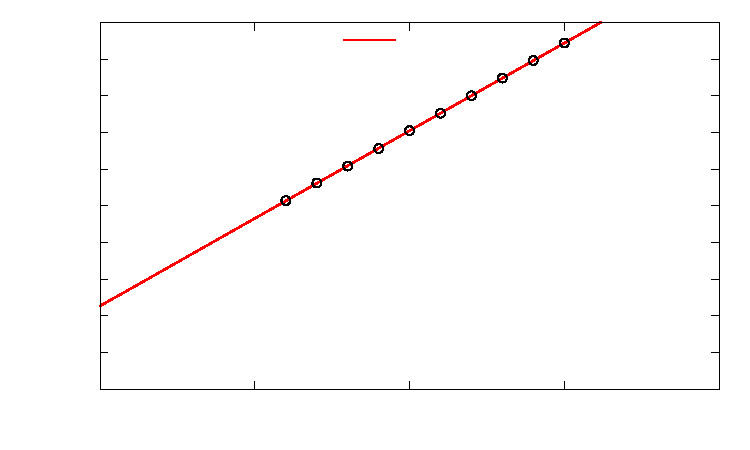
\includegraphics{GRAPH_fwhm_M-ONeill_linear}}%
    \gplfronttext
  \end{picture}%
\endgroup

				}\endgroup
		\caption{A graph showing angular size of target galaxy as a function of redshift.\label{fig:redshift_vs_angular_size}}
	\end{figure}

	This clearly shows a linear trend allowing us to set the FWHM as a simple function of redshift,
	\begin{align}
		\text{FWHM}= 0.0238z + 0.1133
	\end{align}
	this FWHM function then fits into the CCD equation program. This linear trend matches very well with the theory, as is shown in Figure~\ref{fig:angular_size_function_of_redshift}.
	\begin{figure}[htbp]
		\centering
		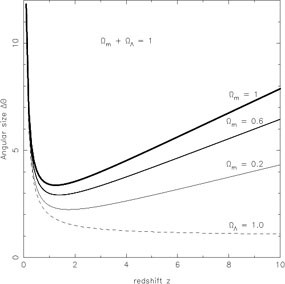
\includegraphics[width=0.5\textwidth]{../Images/angular_size_function_of_redshift.jpeg}
		\caption{A graph showing variation in angular size as a function of redshift\cite{Sahni_FWHM}.\label{fig:angular_size_function_of_redshift}}
	\end{figure}

	Here it can be clearly seen that for the redshifts of interest in this study, between 6--15, the angular size to redshift relation will be in the linear regime. Although this graph does not strictly show $z > 10$, the relation remains linear for a great deal longer and is fully applicable for the majority of the observations proposed in this study.
% subsection full_width_at_half_maximum (end)

    	\subsection{Calculating Exposure Time} % (fold)
	\label{sub:calculating_exposure_time}
		To calculate the exposure time required to view an object at a particular signal-to-noise ratio, the flux density of the source must first be obtained. The flux of the source incident on the CCD can be calculated using the value of apparent magnitude gained from the computational model produced by the Predictions subgroup. This magnitude must first be converted to a flux per unit frequency ($F_\nu$) using equation~(\ref{eq:ab_magnitude}).

		This must then be converted to flux per unit wavelength for use with the properties of the telescope as well as to the required units of \si{\joule\per\second\per\square\centi\metre\per\micro\metre}. This can be done via the formula below. %J/s/cm$^2$/$\mu$m
		\begin{align}
			F_\lambda = \frac{\nu F_\nu \times 10^{-7}}{\lambda} \label{eq:flux_per_unit_frequency}
		\end{align}
		This can then be used to calculate the number of photons striking the primary mirror of the telescope by multiplying this value of flux by the area of the telescopes primary mirror, the bandwidth of the telescope as well as the number of photons per joule of energy. The energy of each photon can be calculated using the wavelength of the incoming photon via $E = \frac{hc}{\lambda}$ and the reciprocal of this value will then give the number of photons per joule of energy. The wavelength of the incoming photon is dependent on the redshift of the source via equation~(\ref{eq:spectroscopy}). The number of photons reaching the CCD can then be calculated by multiplying the number of photons reaching the primary mirror by the throughput of the filter as well as the reflectivity of each mirror the photon must reflect off before reaching the CCD. A rearranged form of the CCD equation, shown below, can then be utilised to calculate an exposure time required to view a given source.
		\begin{align}
			F^2 t^2 - (\frac{S}{N})(F + BN_\text{pix} + DN_\text{pix})t - (\frac{S}{N})R{^2}N_\text{pix} = 0
		\end{align}
		The quadratic formula can then be used to calculate a value of exposure time $t$ in seconds. For ground based telescopes that are background limited, i.e.\ they receive more photons from background than from the source, this calculation of exposure using the CCD equation can be slightly simplified to:
		\begin{align}
			t = (\frac{S}{N})^2 \frac{BN}{F^2}
		\end{align}
		A program was created to complete these calculations incorporating the above equations for various sources and provide the exposure times required for numerous telescopes. These values were then used to determine the suitability of the numerous telescopes for observing high redshift galaxies from the start of the epoch of re-ionisation along with galaxies formed at the end of the EoR. These exposure times calculated are the time required to produce an image with a certain signal-to-noise ratio in one band and so a further 2 or 3 observations must be taken in different bands to confirm the redshift of the galaxies via the dropout method.
	% subsection calculating_exposure_time (end)

	\subsection{Overhead Times} % (fold)
	\label{sub:overhead_times}
		There are many factors that contribute to the time required with a telescope to view a chosen object. Time required with the shutters of the telescope closed is regarded as an overhead time and must be considered during the final observational strategy. This includes time for each of the following\cite{Overhead_Times}:
		\begin{itemize}
			\item Telescope Alignment
			\item Changing filters. This usally requires a time of around 1 minute however this may differ for different instruments.
			\item Changing CCDs to avoid loss of data due to cosmic ray events. Cosmic ray events contribute photons that contaminate pixels in the CCD meaning the image is also slightly contaminated. To avoid this, exposure time is normally split up into a number of separate exposures thus minimising the contamination due to cosmic rays. This can normally be set using a CR-SPLIT option which allocates a fraction of the exposure time to each exposure\cite{Space_Telescope_Science_cosmic_rays}. Importantly, cosmic rays have less impact during observations of small targets such as the galaxies being observed during this project. The splitting of the total exposure time into separate exposures also means an overhead time to replace the CCDs must be considered during the final observing strategy.
			\item Clearing the CCD. The CCD is cleared before every exposure and takes approximately 16\,seconds.
			\item Readout of the CCD. The readout time for a CCD is generally around one minte but increases for exposures of longer than 180\,seconds. This readout time is for one CCD and so must be multiplied by the number of CCDs used  during the exposure. The number of exposures will be increased if the CR-SPLIT option is used.
			%\item Dithering. This is a technique used in photometry whereby the pointing is adjusted a small amount between exposures. This technique's primary use it to account for dead pixels in the CCD; with adjustments of a few pixels the median stacking of the images means that any such defects will disappear. The technique also compensates for the presence of cosmic rays as well as undersampled images; where the sampling frequency is less than twice the highest frequency in the signal (Nyquist Theorem). Dithering also has the benefit of randomising the quantization error that occurs during the analogue-digital conversion of the signal\cite{ADC_Kamensky}. Using a digital image processing method called ``DRIZZLE'', originally developed for use in the Hubble Deep Field, the dithered images can be combined to produce more accurate observations for a given S/N [DRIZZLE].
			\item Transmission of data to Earth from a space based telescope
		\end{itemize}
		Overhead times are extremely difficult to determine quantitatively with times for each of these overheads varying considerably depending on circumstance and the instrument or telescope used. During the final observational strategy for this project, an additional overhead time of 10\% of the required exposure time will be allocated.
	% subsection overhead_times (end)
	\subsection{Dithering} % (fold)
	\label{sub:dithering}
		Dithering is a technique used in photometry whereby the pointing is adjusted a small amount between exposures. This technique's primary use it to account for dead pixels in the CCD; with adjustments of a few pixels the median stacking of the images means that any such defects will disappear. The technique also compensates for the presence of cosmic rays as well as undersampled images; where the sampling frequency is less than twice the highest frequency in the signal (Nyquist Theorem). Dithering also has the benefit of randomising the quantization error that occurs during the analogue-digital conversion of the signal\cite{ADC_Kamensky}. Using a digital image processing method called ``DRIZZLE'', originally developed for use in the Hubble Deep Field, the dithered images can be combined to produce more accurate observations for a given S/N\cite{???}[DRIZZLE].
	% subsection dithering (end)


    \section{Ground Based versus Space Based Telescopes} % (fold)
\label{sec:ground_based_versus_space_based_telescopes}
	Ground based telescopes are seeing limited which is a resolving limitation due to distortion caused by the atmosphere. Light is scattered by the atmosphere and so detecting a source by these telescopes can be difficult. There is also the limitation of considerably more background light, compared to what is measured by space telescopes. To minimise these limitations, ground based telescopes are usually located at high altitude at locations such as Mauna Kea, Hawaii. The main advantage of ground based telescopes is that they can be built to very large sizes with telescopes with a primary diameter of around 30\,metres on the periphery. This cannot be achieved by space telescopes as the cost of transport to space would be very large and the telescope may well be damaged during this transportation.

	Space based telescopes are diffraction limited, i.e.\ the only limitation is whether they can resolve the object being observed. Taking the source as a point spread function, the light from the source will spread out and so the telescope must determine the source. This is important as light from other sources in the sky may almost overlap and so the diffraction gives the angle in the sky which can be resolved. Thus if the diffraction angle, the smallest angle between two objects can be resolved, is small, the better the telescope. Should two sources fall within this diffraction angle when looking into the sky, the telescope will not be able to resolve the two objects and so one cannot be distinguished from another. The diffraction angle can be calculated using the formula below:
	\begin{align}
		\Delta\theta= \frac{(1.22 \lambda)}D
	\end{align}

	This also shows that the larger the diameter, the smaller the diffraction angle will be and so the better the telescope will be at resolving sources.

	The main disadvantage of space based telescope is that they must be transported into space. This is usually done with the aid of a rocket and so the cost of achieving this can be considerable. The telescope may also be damaged during this transportation and so this limits the size of the telescope as a smaller size will mean a smaller chance of being damaged. The James Webb Space Telescope scheduled for launch in 2018 consists of a 6.5 metre primary mirror made up of multiple mirrors that will unfold once it is in space. Despite this folding up of the telescope, the primary mirror size is still small relative to some ground based ones currently in use such as the VLT (primary mirror of 8.2\,metres) and is considerably smaller than some proposed for the future such as the EELT (primary mirror 39.3\,metres).


	\subsection{Astronomical Seeing} % (fold)
	\label{sub:astronomical_seeing}
		Plane waves from a source being observed are distorted by the Earth’s atmosphere and so upon reaching a telescope within the atmosphere are slightly perturbed and so the image formed is blurred. This effect is contributed to by numerous layers where different temperatures or the interaction of different wind speed causes this effect with ‘Seeing’ the term used to describe the total distortion of the wavefront\cite[page~188]{Diffraction_Limited_Imaging_Saha}. This effect is shown below in figure~\ref{fig:Seeing} where a turbulent layer of the atmosphere causes a change in the shape of the wavefront.
		\begin{figure}[ht]
			\centering
			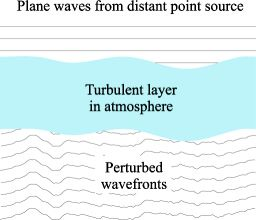
\includegraphics[width=0.4\textwidth]{../Images/Seeing.png}
			\caption{Figure 1}\label{fig:Seeing}
		\end{figure}

		Whilst the resolving power of a telescope is generally largely dependent on its diameter, this seeing limitation becomes the major source of error when resolving a point source from within the Earth’s atmosphere. This is consequently the main limitation for ground based telescopes which are therefore known as being seeing limited. A point spread function (PSF) imaged in these circumstances produces what is known as a seeing disc due to the atmospheric turbulence and the most common measurement used to describe this effect is the full width at half maximum, hereafter the FWHM, shown below in figure~\ref{fig:FWHM} where a peak shape is produced by this overall blurring of the source. When measuring the flux arriving at the CCD from a particular source, an area of radius four times the FWHM is recorded over and so a larger value of FWHM also increases the integration time required to observe the source.
		\begin{figure}[ht]
			\centering
			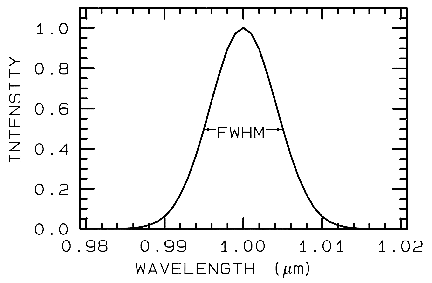
\includegraphics[width=0.5\textwidth]{../Images/FWHM.png}
			\caption{Figure 1}\label{fig:FWHM}
		\end{figure}
	% subsection astronomical_seeing (end)

	\subsection{The Future of Ground Based Telescopes} % (fold)
	\label{sub:the_future_of_ground_based_telescopes}
		The main disadvantage of ground based telescopes compared to space based telescopes is the poorer resolution due to the distortion caused by the atmosphere or astronomical seeing. The introduction of adaptive optics however, should help resolve this issue and allow ground based telescopes to be only diffraction limited similar to space based ones. This, combined with the large diameter mirrors currently in the pipeline such as for the European Extremely Large Telescope (E-ELT), a primary mirror of 39.3 metres, and the Giant Magellan Telescope (GMT), a primary mirror of 25\,metres, ensure ground based telescopes hold a place in the future of space observation, even if just to compliment space based ones. The larger mirrors ensure a greater light collecting power, receiving more photons for the source being observed and so significantly reducing the observing time required. These large diameter mirrors are currently only possible for ground based telescopes and so provide them with a distinct advantage over space based ones.

		\subsubsection{Adaptive Optics} % (fold)
		\label{ssub:adaptive_optics}
			As described earlier in astronomical seeing, light passing through the atmosphere from a source, such as a distant galaxy, is perturbed due to atmospheric turbulence and so the images produced by ground based telescopes are blurred. Adaptive optics works by first sensing the wavefront perturbations and then counteracting this blurring in real time thus enabling the telescopes to hold a much larger resolving power. This system will be used on future ground based telescopes ensuring they are no longer limited by the ability to resolve a source. An example of how this is set up, as on the Subaru Telescope, is shown below in figure~\ref{fig:AdaptiveOptics}.
			\begin{figure}[ht]
				\centering
				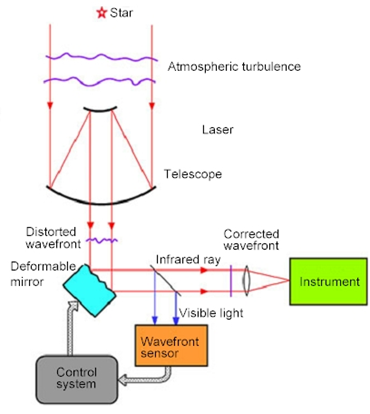
\includegraphics[width=0.6\textwidth]{../Images/AdaptiveOptics.png}
				\caption{Figure 1}\label{fig:AdaptiveOptics}
			\end{figure}

			The wavefront sensor (WFS) measures the distortions in the incoming wavefront of light. This then provides the measured information to an actuator control computer identified in figure~\ref{fig:AdaptiveOptics} as the control system. This then adjusts the shape of the adjustable mirror to effectively correct the wavefront reaching the telescope\cite{Diffraction_Limited_Imaging_Saha}.  The wavefront sensor can measure the distortions introduced into the wavefront on the timescale of a few milliseconds with the information then computed and the shape of the mirror adjusted accordingly. The correction process should therefore be completed in a time similar to the time between the changes of the wavefront thus ensuring the distortion is compensated for.
		% subsubsection adaptive_optics (end)
	% subsection the_future_of_ground_based_telescopes (end)
% section ground_based_versus_space_based_telescopes (end)


\section{Observation Times} % (fold)
\label{sec:observation_times}
	The main aim of this project is to produce an observing strategy to view some of the earliest galaxies in the universe. An important aspect of this is therefore the viewing of the galaxies themselves and the time it will take to do so. The time required to view these galaxies depends not only on the telescope being used, but also the devices used. A charged coupled device (CCD) will be used to measure the light from these sources and so to calculate the times required to view these galaxies, these must be understood in more detail. The telescope or telescopes used during the observation of these galaxies will have different properties which will affect the time required to view the source. Some of these are mentioned below.

	\subsection{Telescope Properties} % (fold)
	\label{sub:telescope_properties}

		\subsubsection{Mirror Reflectivity} % (fold)
		\label{ssub:mirror_reflectivity}
			One such factor that will increase the time required to view a source is the reflectivity of the mirrors used on the telescope. The mirror reflectivity, given as a percentage, is the amount of light reflected by the mirror. Some of the light is absorbed as the mirror is not one hundred per cent efficient meaning not all photons striking the mirror reach the CCD. The reflectivity differs depending on the material used on the surface of the mirrors. Various optical coatings are produced and used depending on the wavelengths being observed, for example, the James Webb Space Telescope uses a gold coating which is particularly useful in the infrared region and also very durable due to the inert nature of Gold. The reflectivity of this gold coated mirror is in the region of 98--99\%\cite{Quantum_Coatings_Incorporated}. Other coatings regularly used include aluminium, which has a reflectivity in the region of 80--90\% and is utilised in the UV and IR range, as well as silver, which has a reflectivity in the range of 95--99\% and is utilised in the visible and IR range.
		% subsubsection mirror_reflectivity (end)

		\subsubsection{Telescope Throughput} % (fold)
		\label{ssub:telescope_throughput}
			The definition of throughput is the ratio of the flux detected by a particular instrument in a given filter and the incoming flux measured over an area equal to the area of the telescope primary mirror\cite{WIRCam_Throughput}. The throughput is therefore the percentage of photons striking the primary mirror that reach the CCD and are recorded. This contributes to the time required to observe a source as not all the photons striking the primary mirror, originated from the source, will reach the CCD. As the number of photons reaching the CCD is fewer, a larger portion of time is required to obtain the sought after signal-to-noise ratio and so the overall observation lasts a longer period of time.
		% subsubsection telescope_throughput (end)

		\subsubsection{Filters}

		\subsubsection{Field of View}
	% subsection telescope_properties (end)

	\subsection{Charged Coupled Devices} % (fold)
	\label{sub:charged_coupled_devices}
		Describe CCD and how it works here.

		The CCD does however have numerous errors known as noise, which contribute to the integration time required to view these early galaxies and so must be taken into account. The conversion of light to pixel values in a CCD leads to an inevitable noise being introduced into the image. This noise is the unwanted variations in pixel values and causes the image produced to differ from the one being observed. The noise incurred will make it more difficult to distinguish the source being observed hence increasing the integration time. For an electrical measuring system such as a CCD, a signal to noise ratio characterises the quality of the measurement taken where the signal to noise ratio (SNR) is the ratio of signal from the source being observed and signal produced by background radiation and other sources of noise. This is generally used to quantify the quality of a CCD measurement. The main sources of noise for a CCD are the dark current, sky background and read noise, which are all described below.
	% subsection charged_coupled_devices (end)

	\subsubsection{Dark Current} % (fold)
	\label{ssub:dark_current}
		Atoms in the silicon substrate of the CCD used are thermally excited and thus electrons are freed. This occurs even when the CCD is not exposed to light, hence there is a steady creation of electrons, and this is called the dark or thermal current. As this is caused by thermal excitation, it strongly depends on the temperature at which the device is operating. At any given temperature, the rate at which electrons are freed is constant, however for every rise in temperature of 6 degrees Celsius, the dark current produced approximately doubles\cite[pages~124--125]{Astronomical_Image_Processing}. This relationship is shown in figure~\ref{fig:dark_current} below\cite{Southern_Observatory_throughput}.
		\begin{figure}[ht]
			\centering
			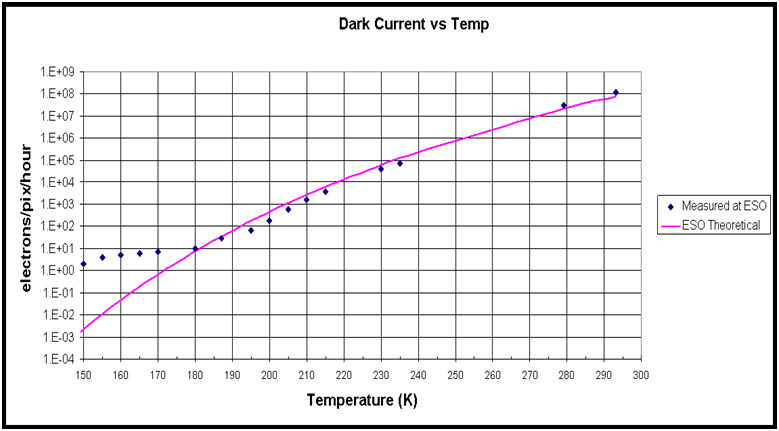
\includegraphics[width=0.7\textwidth]{../Images/Dark.png}
			\caption{Figure 1}\label{fig:dark_current}
		\end{figure}

		Figure 1 shows that relationship between temperature and dark current for a custom designed CCD provided to the European Southern Observatory and shows clearly the increase in dark current at higher temperatures. CCD’s are therefore cooled, often with the use of liquid nitrogen, to minimise this effect. The dark current itself is a relatively small electric current that flows through numerous photosensitive devices, and is one of the main sources of noise for a CCD.
	% subsubsection dark_current (end)

	\subsubsection{Sky Background} % (fold)
	\label{ssub:sky_background}
		The sky background is the incoming light from the sky measured on the telescope that is not from the source being observed. The amount of sky background can vary at different wavelengths and is mainly due to light diffusion by the atmosphere. There are numerous sources that contribute towards the sky background such as airglow and zodiacal light. Airglow is the atmospheric emission of photons at wavelengths from the near-UV to the near-IR range due to chemical reactions in the upper atmosphere\cite[page~9]{atmospheric_radiation_model}. These chemical reactions lead to light emission due to the decay of electrons from an excited state in one of the reaction products. One such example is the emission in the near infrared region by OH radicals created from a reaction between ozone and hydrogen in the upper atmosphere\cite{residual_OH_emission}. Other processes contributing to airglow are the recombination of ions originally ionised by the sun, and the luminescence of cosmic rays striking the upper atmosphere. Thermal radiation in the atmosphere by greenhouse gases also contributes to the sky background and is due to the absorption and emission of radiation from the Sun into the atmosphere in the mid-IR region. In this case, observations in the mid- and far-IR region must be carried out from outside the atmosphere\cite[pages~22--23]{Peter_Schneider_IR}. The sky background is therefore primarily an issue for ground based telescopes as they can incur a large background number of photons compared to the number of photons arriving from the source being observed. As space based telescopes are situated outside of the atmosphere, they avoid almost all of this background.
	% subsubsection sky_background (end)
% section observation_times (end)



\section{Potential Telescopes for Photometry Strategy} % (fold)
    \label{sec:telescopes_chosen_for_investigation}
        %!TEX root = mainfile.tex

\section{The Hubble Space Telescope} % (fold)
\label{sec:the_hubble_space_telescope}

	\subsection{Mission Launch} % (fold)
	\label{ssub:mission_launch}
		On April 24th 1990 NASA’s Space Shuttle Discovery launched the world’s first space-based optical telescope; The Hubble Space Telescope (HST), named in honour of American astronomer Edwin P. Hubble. Edwin Hubble’s greatest contribution to astronomy was the Hubble Law which states that galaxies are receding from us at a speed directly proportional to their distance from us. This showed that our universe is expanding, a notion which underpins modern cosmological thinking. The telescope sits in a low-Earth orbit, as shown in figure~\ref{fig:hubble_space_telescope}, at an altitude of 569 kilometres completing one orbit of the Earth every 97\,minutes\cite{Hubsite_1}.
		\begin{figure}[ht]
			\centering
			\includegraphics[width=0.5\textwidth]{../Images/Hubble_Space_Telescope.jpg}
			\caption{Photograph of HST orbiting the Earth.\label{fig:hubble_space_telescope}}
		\end{figure}

		The HST was designed to provide clear and deep views of distant galaxies and stars and most of the planets in our solar system. Hubble's domain extends from the ultraviolet through the visible and into the near-infrared\cite{NASA_1}.
	% subsection mission_launch (end)

	\subsection{Achievements to Date} % (fold)
	\label{ssub:achievements_to_date}
		The HST has provided unprecedented detail in images of star formation allowing astronomers to see the jets and disks present during the birth of new stars. It has also been able to study the atmospheric composition of extra-solar planets and take the first visible light picture of a planet outside our solar system; Fomalhaut b\cite{Hubsite_3}.

		Many EoR galaxies and candidate galaxies have been identified using HST data. In December 1995 the HST was pointed at what was believed to be a fairly empty and uninteresting patch of sky; 342 separate exposures were taken over 10 consecutive days and formed an image called the Hubble Deep Field (HDF)\cite{ESA_2}. The image contains around 3,000 objects of which the vast majority are galaxies, with a few local stars in the foreground. The HDF is one of the most iconic images of the 20th century, and it has since been cited in over 800 scientific papers.

		In 2004 its successor was revealed, the Hubble Ultra Deep Field (UDF); a million-second exposure in a 200\si{\arcsecond}$\times$200\si{\arcsecond} area of sky containing \num{10000} galaxies stretching back 13\,billion years\cite{Hubsite_2}. This exposure utilised the recently installed Advanced Camera for Surveys (ACS), seen in figure~\ref{fig:HUDF}. This survey was further refined in September 2012 in the Hubble eXtreme Deep Field (XDF) which utilised the recently installed WFC3 camera as well as combining over \num{2000} separate exposures from different sources\cite{ESA_2}.
		\begin{figure}[ht]
			\centering
			\includegraphics[width=0.8\textwidth]{../Images/HUDF.png}
			\caption{The HUbble Ultra Deep Field.\label{fig:HUDF}}
		\end{figure}

		Using data from the HUDF, object UDFj-39546284 was identified. In a paper by Bouwens et al, published in 2012, their best fit places it at a redshift of $11.8\pm0.3$\cite{Bouwens2012}. This would classify it as the oldest object ever observed. The exact nature of the object is not known but it is believed to be a mini-galaxy. Confirmation will require spectroscopic analysis, which is likely to be carried out by the James Webb Space Telescope. This observation demonstrates both the achievements and limits of the current technology.
	% subsection achievements_to_date (end)

	\subsection{Operation} % (fold)
	\label{ssub:operation}
		The HST is operated remotely from the earth, it has 4 antennae which can send and receive signals from the Flight Operations Team at Goddard Space Flight Centre in Greenbelt, Maryland via the Tracking and Data Relay Satellite system. For communication to be possible HST must have a direct line of sight to at least one of these 5 satellites.

		The HST is powered using 2 arrays of solar panels each capable of converting the Sun’s rays into \num{2800} watts of electricity. The arrays are able to store the electricity in batteries allowing the HST to remain active while in the Earth’s shadow (approximately 36\,minutes out of every 97\,minute orbit).

		Orbiting the Earth subjects the HST to extreme conditions due to the effect of zero gravity and the variation in temperature (up to around \SI{40}{\kelvin}) during each orbit. The optical system is held together using a skeleton (truss) constructed from Graphite epoxy. Graphite epoxy, commonly found in racquets and golf clubs is a stiff and lightweight material able to resist expansion and contraction due to temperature changes\cite{Hubsite_4}.
	% subsection operation (end)

	\subsection{Performance and Optical Telescope Array} % (fold)
	\label{ssub:performance_and_optical_telescope_array}
		The HST is constructed using a Ritchey-Chretien Cassegrain design; this allows high-performance over a wide field of view. The incoming light enters a tube with baffles removing any unwanted stray light, as shown in figure~\ref{fig:HST_optical_diagram} below. The light is then collected by the concave Primary mirror and reflected towards the smaller convex Secondary mirror. This light is then reflected back through a hole in the centre of the Primary mirror where it is focused onto a small area to be picked up by the instruments\cite{Hubsite_5}.
		\begin{figure}[ht]
			\centering
			\includegraphics[width=0.5\textwidth]{../Images/HST_optical_diagram.jpg}
			\caption{Diagram showing basic systems of HST, note that WFC2 has since been replaced by WFC3.\label{fig:HST_optical_diagram}}
		\end{figure}

		The mirrors have been polished to an accuracy of better than the wavelength of visible light. When the HST was first launched the scientists soon realised that the curve to which the mirrors had been ground was not correct resulting in an error known as spherical aberration which blurred the images. A servicing mission in December 1993 deployed 5 pairs of mirrors which were able to successfully correct the error and allow Hubble to take the images it was intended to\cite{ESA_1}.

		There have been 4 servicing missions sent to the HST with the final mission taking place in May 2009. Over its lifetime the cameras and instruments have undergone many improvements and replacements. The camera currently operating that is of interest to this project is the WFC3/IR camera, installed in 2009. This camera is able to observe in the near-infra-red where we expect to see the Lyman-break galaxies. Table~\ref{tab:HST_technical} shows the key technical data for the HST, amazingly the HST is so precise it is able to lock onto a target at a distance of 1 mile without deviating more than the width of a human hair.
		\begin{table}[ht]
			\begin{center}
				\begin{tabular}{l|l}
					Component	& 	Details \\
					\hline\hline
					Primary Mirror Diameter & \SI{2.4}{\metre} \\ \hline
					Secondary Mirror Diameter & \SI{0.3}{\metre} \\ \hline
					Wavelength range & 800--1700\si{\nano\metre} \\ \hline
					Total Field of View & \SI{123}{\arcsecond}$\times$\SI{136}{\arcsecond} (\SI{16728}{\arcsecond}$^2$) \\ \hline
					Pixel Size & $18\times18$\,\si{\micro\metre} \\ \hline
					Plate Scale & \SI{0.13}{\arcsecond\per\pixel} \\ \hline
					\multirow{3}{*}{Quantum Efficiency} & 77\% at \SI{1000}{\nano\metre}\\
					 & 79\% at \SI{1400}{\nano\metre}\\
					 & 79\% at \SI{1650}{\nano\metre}\\ \hline
					Dark count &  \SI{0.048}{\electron\per\second\per\pixel} \\ \hline
					Readout noise & \SI{12.0}{\electron\per\second\per\pixel} \\ \hline
					Full Well & \SI{77900}{\electron} \\ \hline
					Gain & 2.28--2.47\si{\electron\per\ADU} \\ \hline
					Operating Temperature & \SI{145}{\kelvin} \\ \hline
					FWHM & \SI{0.151}{\arcminute} at \SI{1600}{\nano\metre}
				\end{tabular}
			\end{center}
			\caption{Technical data for HST WFC3/IR camera system\cite{WFC3_IHB}}
		\label{tab:HST_technical}
		\end{table}
	% subsection performance_and_optical_telescope_array (end)

% section the_hubble_space_telescope (end)

        %!TEX root = mainfile.tex

\subsection{Spitzer Space Telescope} % (fold)
\label{sub:spitzer_space_telescope}
(Dorothy with contributions from Catherine)

	Spitzer Space telescope was launched by NASA on 25th August 2003\cite{fast_facts_spitzer} and is designed for use in the infrared. It was the last of NASA's ``Great Observatories'', working alongside HST in the optical, Compton Gamma Ray Observatory and Chandra X-ray Observatory. The telescope is \SI{85}{\centi\metre} in diameter, and sits in an Earth-trailing orbit around the Sun, shown in Figure~\ref{fig:spitzer_orbit_LARGE}. It is a Cassegrain telescope, meaning it has primary and secondary hyperbolic mirrors to focus the light and reduce spherical aberration, in a similar manner to Hubble. The majority of Spitzer's instrumentation is now non-operational due to a lack of cryogen, but some photometry remains possible.
	\begin{figure}[htbp]
		\centering
		\includegraphics[trim = 110mm 70mm 5mm 30mm, clip, width=0.6\textwidth]{../Images/spitzer_orbit_LARGE.png}
		\caption{The Spitzer Space Telescope's Orbit\cite{where_is_spitzer}.\label{fig:spitzer_orbit_LARGE}}
	\end{figure}

	\subsubsection{Capabilities} % (fold)
	\label{ssub:spitzer_capabilities}
		Spitzer had the capabilities detailed in Table~\ref{tab:Spitzer_cababilities}.
		\begin{table}[htbp]
			\begin{center}
				\begin{tabular}{l|l}
					Component   &   Wavelength Range \\
					\hline\hline
					Imaging/Photometry & 3--180\si{\micro\metre} \\
					Spectroscopy       & 5--40\si{\micro\metre} \\
					Spectrophotometry  & 50--100\si{\micro\metre}
				\end{tabular}
			\end{center}
			\caption{Details of instrumentation for Spitzer\cite{WFC3_IHB}.\label{tab:Spitzer_cababilities}}
		\end{table}

		It employed three scientific instruments which helped it do the above:
		\begin{itemize}
			\item Infrared Array Camera (IRAC): an imaging camera working in the near IR at wavelengths of 3.6, 4.5, 5.8 and 8\,micrometres.
			\item Infrared Spectrograph (IRS): performing spectroscopy from 5 to 40\,micrometres.
			\item Multiband Imaging Photometer (MIPS): detected wavelengths in the far IR, at 24, 70 and 160\,micrometres.
		\end{itemize}

		The telescope was cryogenically cooled to around \SI{1.4}{\kelvin}, allowing all the instruments to function without excessive thermal interference from the telescope itself. The mission, labelled the `Cold Mission', was estimated to last between 2 and 5 years, depending on when the cryogen ran out. During this time, Spitzer imaged in all four NIR filters simultaneously, as well as doing spectroscopy, and some imaging in the far infrared. In 2009, when the cryogen ran out, the longer wavelength filters became non-operational, and the Spitzer `Warm Mission' continued imaging with the nearest IR filters ($3.6$ and $4.5$\,micrometres). This was made possible because Spitzer's orbit keeps it substantially cooler than an Earth-centred orbit would, due to the lack of IR radiation received from Earth. Furthermore it is made mostly of beryllium which has a low heat capacity at low temperatures, helping to keep it cool.

		In order to keep enough sunlight on the solar panels, Spitzer cannot point further than 120\,degrees away from the Sun. However, it also cannot get closer than 80\,degrees towards the Sun in case damage is done to the scientific instruments. This is a limitation on the area of sky which can be observed, meaning that some regions can only be seen for 40 days semi-annually, whilst other areas can be observed all year round.

		The spectrograph (IRS) operated at wavelengths too long to be of use to study the EoR, as did the far IR photometry (MIPS), however the near IR photometry capabilities of both the Spitzer warm and cold missions have been used to study high redshift galaxies, and in conjunction with HST have confirmed galaxies at redshifts as far back as $z\approx10$. Particularly the 3.6 and 4.5\,micrometre filters observe significant flux from such galaxies, and so these have been used in a number of studies looking for high redshift galaxies.
	% subsubsection capabilities (end)

	\subsubsection{Studies involving Spitzer} % (fold)
	\label{ssub:studies_involving_spitzer}
		Coe et al (2012)\cite{0004-637X-762-1-32} reports a $z\approx11$ candidate which had been observed using HST (WFC3, ACS) and Spitzer (IRAC) for longer wavelengths. This is one of the highest redshift candidates to date. The Spitzer data was taken over a total integration time of 5 hours.

		An earlier study in 2008 by Richard et al also used Hubble to detect galaxies greater than redshift seven (making use of gravitational lenses). Spitzer imaged these galaxies to help confirm that they were not foreground objects of a different nature, by looking at the flux in longer wavelength filters\cite{0004-637X-685-2-705}.

		In 2005, during the cold mission, a study was made by Spitzer on a confirmed $z=6.56$ galaxy (HCM 6A) lensed by a cluster (Abell 370). The study was used to detect the rest frame optical emission of this galaxy in order to better understand the physical properties of objects at such high redshifts\cite{1538-4357-635-1-L5}. Several other papers have also used Spitzer data in the study of high redshift galaxies.

		Spitzer also has ideal filters to look at the Balmer or \SI{4000}{\angstrom} break which, if prominent, would indicate an older stellar population and suggest that the object is more likely a contaminant than a high redshift LBG, since high redshift LBGs do not contain many old stars.

		The data in Table~\ref{tab:Spitzer_technical} shows some of the key technical data availible for the telescope.
		\begin{table}[htbp]
			\begin{center}
				\begin{tabular}{l|l}
					Component   &   Details \\
					\hline\hline
					Primary mirror & \SI{0.85}{\metre} \\
					FoV & \SI{5.2}{\arcminute}$\times$\SI{5.2}{\arcminute} \\
					Pixel size & \SI{1.2}{\arcsecond}$\times$\SI{1.2}{\arcsecond} \\
					Detector Array & $256\times256$\,\si{\pixel} \\
					\multirow{2}{*}{Full well} & 145,000 at \SI{3.6}{\micro\metre} \\
							& 140,000 at \SI{4.5}{\micro\metre} \\
				\end{tabular}
			\end{center}
			\caption{Technical data for Spitzer\cite{Spitzer_Heritage_Archive_Documentation}.\label{tab:Spitzer_technical}}
		\end{table}
	% subsubsection studies_involving_spitzer (end)
% subsection spitzer_space_telescope (end)

        %!TEX root = mainfile.tex

\subsection{Euclid} % (fold)
\label{sub:euclid}

	\subsubsection{Mission Overview} % (fold)
	\label{ssub:mission_overview}
		The Euclid mission is planned for launch in 2020, at an estimated total cost of 800\,million Euros\cite{bbc_euclid}. Its primary goal is to conduct a wide survey; some 15000 degrees of sky is planned to be covered. There is also to be a deep survey which is expected to cover around 40 degrees to a depth 2 magnitudes deeper than the wide survey. It will have a near infra-red camera and spectrometer as well as an optical camera. The primary mission  objectives are expected to be completed within 7 years. One of Euclid’s main scientific objectives with the deep field is to study high redshift galaxies at z =6+ over a very wide survey area. This will give astronomers the opportunity to spectroscopically confirm hundreds of galaxies for use in the study of the EoR. It will help constrain the bright end of the luminosity function at high z.
	% subsubsection mission_overview (end)

	\subsubsection{Capabilities} % (fold)
	\label{ssub:capabilities}
		\begin{itemize}
			\item Visual Imaging/ Photometry, 550--900\si{\nano\metre}
			\item Spectroscopy, 1100--2000\si{\nano\metre}
			\item NIR Imaging/ Photometry, 920--2000\si{\nano\metre} (Y, J,H bands)
		\end{itemize}

		Euclid will have two instruments in order to do the above; a wide-band imaging system in the visible (VIS), and an instrument capable of both slit-less spectroscopy as well as NIR imaging. These instruments will be operated simultaneously.
	% subsubsection capabilities (end)

	\subsubsection{Key Technical Data} % (fold)
	\label{ssub:key_technical_data}
		The data in table~\ref{tab:Euclid_technical} is quoted for the deep survey NIR photometry. Some data is subject to slight change as the planning stages progress.
		\begin{table}[ht]
			\begin{center}
				\begin{tabular}{l|l}
					Component & Details \\
					\hline\hline
					Primary mirror		& \SI{1.2}{\metre} \\ \hline
					FoV 				& $0.763\times0.763$\si{\degree\squared} \\ \hline
					Pixel size			& \SI{0.3}{\arcsecond}$\times$\SI{0.3}{\arcsecond} \\ \hline
					Detector Array		& \num{2000}$\times$\num{2000}\,\si{\pixel} \\ \hline
					Resolution 			& 0.3 to \SI{0.6}{\arcsecond} (in J band) \\ \hline
					Plate Scale (infra-red)	& \SI{0.3}{\arcsecond\per\pixel}
				\end{tabular}
			\end{center}
			\caption{Technical data for HST WFC3/IR camera system\cite{WFC3_IHB}.\label{tab:Euclid_technical}}
		\end{table}
	% subsubsection key_technical_data (end)
% subsection euclid (end)

        %!TEX root = mainfile.tex

\subsection{European Extremely Large Telescope} % (fold)
\label{sub:european_extremely_large_telescope}
	One of a new generation of ground based telescopes, the European Extremely Large Telescope (E-ELT), shown in figure~\ref{fig:artist_eelt}, is scheduled for first light in 2022 and has a projected lifetime of 30 years, although major upgrades are expected during this period\cite[p.~163]{E_ELT_Construction_Proposal}, and an estimated cost of around 1083\,million Euros. The Telescope will be constructed on Cerro Armazones in Chile at an altitude of approximately \SI{3060}{\metre} and will be part of the La Silla Paranal observatory. With a primary mirror diameter of \SI{39.9}{\metre}, the E-ELT will be the largest optical/near-infrared telescope in the world. The telescope will also incorporate adaptive optics, discussed in section~\ref{ssub:adaptive_optics}, which will result in it being able to correct for atmospheric perturbations and therefore be diffraction limited.
	\begin{figure}[!htb]
		\centering
		\includegraphics[width=0.6\textwidth]{../Images/E-ELT.png}
		\caption{An artist's impression of the E-ELT\cite{E_ELT_Enclosure}}\label{fig:artist_eelt}
	\end{figure}

	One of the most important components of the E-ELT is the dome within which the telescope is enclosed. This primarily provides protection to the telescope against unfavourable weather conditions and during the day. The dome is designed to allow complete freedom to the telescope, allowing it to position itself, permitting observations between a $20^{\circ}$ angle to the horizon and zenith and also incorporates a windscreen protecting the mirrors. As well as being water-tight, the dome is also air-tight to minimise the air-conditioning load. The E-ELT will use an air-conditioning system to cool the mirror and instrumentation to ensure optimum operating conditions in preparation for the upcoming night.

	The E-ELT utilises a three mirror anastigmat system with two further mirrors providing the adaptive optics, shown below in figure~\ref{fig:5_mirror_eelt}, with the fifth mirror directing the beam towards the Nasmyth focus\cite[p.~16]{E_ELT_Construction_Proposal}. The primary mirror, measuring \SI{39.3}{\metre} in diameter, will be comprised of 798 hexagonal segments eventually producing a collecting area of \SI{978}{\square\metre}. The E-ELT will therefore have a light collecting power approximately 13 times larger than any existing telescope and is predicted to produce images 16 times sharper than those of the Hubble Space Telescope. Other new generation extremely large telescopes include the Giant Magellan Telescope with a primary mirror of diameter \SI{25}{\metre} and the Thirty Metre Telescope with a primary mirror of diameter \SI{30}{\metre}. The E-ELT however remains the largest of these planned telescopes.
	\begin{figure}[!htb]
		\centering
		\includegraphics[width=0.6\textwidth]{../Images/Anastigmat.png}
		\caption{The 5 mirror design to be utilised on the E-ELT}\label{fig:5_mirror_eelt}
	\end{figure}

	\subsubsection{Main Aims} % (fold)
	\label{ssub:main_aims}
		One of the main aims of the E-ELT will be the search for extra-solar planets.  This will include the detection of extra-solar planets using the radial velocity technique, the detection of variations of the radial velocity of a star with respect to the Earth in response to the gravity of an orbiting planet, as well as possible direct imaging of larger planets. The E-ELT may also be used to characterise the atmosphere of these larger planets using low resolution spectroscopy. The observation of giant planets in star forming regions and young stellar clusters will also provide an insight into their evolution.

		Another of the main aims is the study of the universe at high redshift. The E-ELT will look back at the earliest galaxies formed after the ``dark ages'', the galaxies therefore responsible for the re-ionisation of the universe. Properties of these early galaxies including their star formation rates, ages, metallicities and stellar masses will be determined contributing to a better understanding of galaxy formation and evolution.

		The E-ELT will also help to understand the nature of dark energy through the discovery and identification of type 1a supernovae. As these are excellent distance indicators, they can be used to map space and its expansion history thus providing information on what is believed to be the source of this expansion. The E-ELT will also attempt to measure small time-drifts in the redshifts of distant objects in the intergalactic medium, a consequence of the evolution the universal expansion rate. The E-ELT will also attempt to discover variations of physical constants over time which, if found to be the case, will have great consequences on our understanding of the general laws of physics.
	% subsubsection main_aims (end)

	\subsubsection{Instrumentation} % (fold)
	\label{ssub:instrumentation}
		At first light, the E-ELT will have just two instruments\cite{E_ELT_Instrumentation}, a diffraction-limited near-infrared imager (MICADO) as well as a single-field near-infrared wide-band integral field spectrograph (HARMONI). Three further objects, a mid-infrared imager and spectrometer (METIS), a high-resolution spectrometer (SIMPLE) and multi-object spectrometer (OPTIMOS) will be added soon after first light\cite{E_ELT_Instrumentation}. There are also some other concepts being studied for use on the E-ELT including a planet imager with extreme adaptive optics (EPICS). Importantly, the instrumentation available will mean that the E-ELT can be used for both photometry and spectroscopy and is also said to be able to switch between these instruments in a matter of minutes.
	% subsubsection instrumentation (end)
% subsection european_extremely_large_telescope (end)

        %!TEX root = mainfile.tex

\subsection{James Webb Space Telescope} % (fold)
\label{sub:james_webb_space_telescope}
	The James Webb Space Telescope (JWST) is a near-infrared space based telescope. Formerly known as the Next Generation Space Telescope, it was renamed after the NASA administrator James Edwin Webb in 2002. It is an international collaboration between NASA, the European Space Agency (ESA) and the Canadian Space Agency (CSA). The JWST’s capabilities will enable a broad range of investigations across many different fields in astronomy. However, its primary goal is to observe the most distant objects in our universe that are beyond the reach of any current ground or spaced based instruments. More importantly for our specific goals it will enable the study of the epoch of re-ionisation and the first stars\cite{primary_mirror_construction}.

	The JWST consists of four main instrument components:
	\begin{itemize}
		\item Near-Infrared Camera (NIRCam),
		\item Near-Infrared Spectrograph (NIRSpec),
		\item Mid-Infrared Instrument,
		\item Fine Guidance Sensor.
	\end{itemize}

	NIRCam uses a technique of CCD photometry to measure the magnitude of high redshift galaxies. It consists of ten mercury-cadmium-telluride (HgCdTe) detector arrays which are analogous to CCD’s found in digital cameras. Coronagraphs enable NIRCam to collate images of very faint objects around a central bright object\cite{primary_mirror_construction}.

	NIRSpec enables the JWST to obtain the spectrums of high redshift galaxies. It is comprised of micro shutter array with \num{62000} shutters that can be closed and opened individually meaning that the JWST can record the spectrums of one hundred different objects simultaneously. The device will have a total field of view of $3\times3$ arcminutes. As well as the micro shutter array NIRSpec will also have five fixed slits for high constant spectroscopy. There is an integral field unit spectrograph (IFU) with thirty slicers meaning that the spectrums of extended bodies can be found. The wavelength range over which NIRSpec can successfully operate is \SI{0.6}{\micro\metre} to \SI{5}{\micro\metre}\cite{primary_mirror_construction}.

	The Mid-Infrared Instrument will be used to obtain the spectrums of objects similar to NIRSpec. However the range over which it will operate will be \SI{5}{\micro\metre} to \SI{29}{\micro\metre}\cite{primary_mirror_construction}.

	Fine Guidance sensor (FGS) is a sensitive camera that will provide critical information for the JWST’s altitude control system. Its main functions include obtaining images for target acquisition and providing guide stars for the alignment and phasing for the segments of the primary mirror\cite{stsci_edu}.

	The JWST’s primary advantage over other current (and planned) space telescopes is its large primary mirror which has a diameter of 6.5\,metres. The next largest mirror of any spaced based telescope belongs to the Hubble Space Telescope (HST) which has a diameter of 2.4\,metres. JWST’s primary mirror is fabricated from eighteen beryllium segments each with a diameter 1.3\,metres which when correctly phased together act as a single mirror. The mirror phasing is achieved due to the fact that every segment has six degrees of rotational freedom by way actuators attached to their underside and the back plane. The back plane holds the primary mirror structure together\cite[p.~568--569]{gardner2006james}.
	\begin{figure}[!htbp]
		\centering
			\includegraphics[width=0.6\textwidth]{../Images/JWST_mirror_construction.jpeg}
		\caption{\cite{primary_mirror_construction}\label{fig:james_web_layout}}
	\end{figure}

	The adjustability of JWST’s primary mirror allows for active optics, as discussed in Section~\ref{ssub:adaptive_optics}. When a mirror of this size pivots to look at different portions of space it naturally bends and deforms. By focusing on a reference object this deformity can be constantly corrected using the actuators connected to each segment of the primary mirror. It will be coated in gold to ensure a maximum reflectivity of 98\%\cite{mtwilson}.

	The Orbit of the JWST will lie at the second Lagrange point (L2) \SI{150000}{\kilo\metre} from Earth. L2 is one of five solutions to the three body problem posed by Joseph Louie Lagrange. It means that when the JWST is in orbit, the sun moon and earth will all stay in the same position relative to each other. The orbit is slightly inclined with respect to the elliptical plane, avoiding moon and earth eclipses of the sun, thus ensuring continuous electrical power is supplied. Orbit shown below in figure~\ref{fig:james_web_orbit}\cite{primary_mirror_construction}.
	\begin{figure}[!htbp]
		\centering
			\includegraphics[width=0.5\textwidth]{../Images/JWST_orbit_L2.jpeg}
		\caption{Diagram of the orbit of the James Webb Space Telescope\label{fig:james_web_orbit}}
	\end{figure}

	The JWST is fitted with a sunshield which reduces the incident radiation of approximately 200 KW to a few milliwatts. This solar attenuation is achieved through the five layer design of the sunshield. Each layer is separated from the next via a vacuum which allows for passive cooling of the JWST. The sunshield will a surface area of approximately \SI{250}{\square\metre} which is too large to fit inside any current spacecraft so will be unfolded into position once the JWST is in orbit at L2. Due to this size, solar radiation will cause a build-up of angular momentum throughout its service. This will be offset by firing service thrusters used primarily for obit maintenance.

	The JWST is a three mirror anastigmat meaning it can minimize the three main optical aberrations, namely; spherical aberration, coma and astigmatism. The effective focal length of the mirrors combined is \SI{131.4}{\metre}. The basic layout can be seen in Figure~\ref{fig:james_web_layout}.

	For the most part the JWST will be background limited as opposed to diffraction limited. The background is due mostly to scattered zodiacal light, scattered starlight and thermal emission from the sunshield. The background due to these factors can be seen in Table~\ref{tab:JW_exposure_times_for_galaxies}. The imaging performance of the JWST will be diffraction limited (i.e.\ limited by the optical power of the telescope) at \SI{2}{\micro\metre} with a Strehl ratio greater than 0.80.

	The field of view refers to the fraction of the celestial sphere that the telescope can point at any given moment. The main limitation to the JWST’s field of view is the sunshield means that only 31\% of the sky can be seen for more than 197\,days. All regions of sky have at least 51\,days of continuous visibility per year\cite[p.~561--572]{gardner2006james}.

	Table~\ref{tab:JW_exposure_times_for_galaxies} below shows the information required in order to calculate exposure times for galaxies of given red shifts and magnitudes at a set signal to noise ratio.
	\begin{table}[!htbp]
		\begin{center}
			\begin{tabular}{c|c}
				Read Noise 					& 10 \\
				Dark Current 				& \SI{0.018}{\electron\per\second\per\pixel} \\
				Diameter of Primary Mirror 	& \SI{8.2}{\metre} \\
				Quantum Efficiency 			& 0.8 \\
				Sky Background 				& 0.005\,photon s$^{-1}$pixel$^{-1}$) \\
				Gain 						& 1.8\si{e}ADU$^{-1}$) \\
				Mirror Reflectivity 		& 0.98 \\
				CCD Pixel Number 			& $2048 \times 2048$
			\end{tabular}
		\end{center}
		\caption{Information required in order to calculate exposure times for galaxies of given red shifts and magnitudes.\label{tab:JW_exposure_times_for_galaxies}}
	\end{table}
% subsection james_webb_space_telescope (end)

    % section telescopes_chosen_for_investigation (end)
    	\section{Potential Telescopes for Spectroscopy Strategy} % (fold)
	\label{sub:candidate_telescopes}
		\subsection{James Webb Space Telescope} % (fold)
		\label{ssub:james_webb_space_telescope}
			The primary telescopes considered for use in this research are the JWST and the E-ELT. The JWST’s NIRSpec is a device which will enable the conformation of high red shift galaxies. It uses a combination of slits, prims and gratings to achieve high resolution spectroscopy. Perhaps its most innovative feature is a microshutter array. The microshutters are tiny cells that measure $100 \times 200$\,\si{\micro\metre}. They are arranged over a waffle like grid containing \num{62000} individual cells. NIRSpec will contain four identical grids in total. The cells all have lids which can be opened and closed individually. This is achieved by sweeping a magnet across the surface of the array which opens all of the lids and the electronically closing individual lids. Each cell measures $203 \times 463$\,milliarcseconds. The total field of view for all four arrays combined is $3 \times 3$\,arcminutes. Shutters in each array can be opened or closed to form multiple apertures meaning that spectrums for one hundred different targets can be found simultaneously. The size and shape of the apertures can be selected to obtain the clearest spectrum possible for each individual target. Figures~\ref{fig:nirspec_construction} and~\ref{fig:nirspec_mirrors} show NIRSpec under construction\cite{JWSTPrimer}[8].
			\begin{figure}[!htbp]
				\begin{minipage}[c]{0.5\linewidth}
					\centering
					\includegraphics[width=0.9\textwidth]{../Images/nirspec_construction.jpeg}
					\caption{\label{fig:nirspec_construction}}
				\end{minipage}
				\begin{minipage}[c]{0.5\linewidth}
					\centering
					\includegraphics[width=0.9\textwidth]{../Images/nirspec_mirrors.jpeg}
					\caption{\label{fig:nirspec_mirrors}}
				\end{minipage}
			\end{figure}

			As well as the microshutter array the JWST also contains an integral field unit. Integral field spectroscopy has become an important sub discipline of astronomy where there is a need to study the spectra of extended bodies. This has particular significance as high red shift galaxies are considered to be extended bodies.

			Integral field spectroscopy is the successor to long slit spectroscopy where the spectrum is dispersed perpendicular to the slit direction. By stepping the position of the slit the spectrum of points over the extended body can be obtained. An integral field unit speeds up this process by slicing the image and then rearranging it so that different parts can illuminate the slit. This negates the need to take multiple exposures\cite{INTEGRAL_FIELD_UNIT}.

			NIRSpec will be able to disperse light comprised of wavelengths between 0.6 and 5 microns, i.e. the infrared range over which the Gunn Peterson trough should occur. It will do this using one prism and five diffraction gratings. The wavelength ranges over which each will work and their associated wavelengths are shown below.
			\begin{table}[!htbp]
				\begin{center}
					\begin{tabular}{c|c|c|c}
						Grating & Filter & Resolution & Wavelength (\si{\micro\metre}) \\
						\hline \hline
						Prism & Clear & 100 & 0.5--5 \\
						G140M & F100LP & 1000 & 1.0--1.8 \\
						G235M & F170LP & 1000 & 1.7--3.0 \\
						G395M & F290LP & 1000 & 2.9--5.0 \\
						G140M & F100LP & 2700 & 1.0--1.8 \\
						G235M & F170LP & 2700 & 1.7--3.0 \\
						G395M & F290LP & 2700 & 2.9--5.0
					\end{tabular}
				\end{center}
				\caption{Number of galaxies for set total observing time given different magnitudes/ survey areas for JWST.\label{tab:galaxies_for_set_total_observing_time_JWST}}
			\end{table}
		% subsubsection james_webb_space_telescope (end)

		\subsection{European Extremely Large Telescope} % (fold)
		\label{sub:european_extremely_large_telescope}
			The European-Extremely Large Telescope (E-ELT) will be equipped with three spectroscopic devices:
			\begin{enumerate}
				\item EAGLE - A multichannel integral field near infrared spectrograph with multi object adaptive optics;
				\item HARMONI - A wide band field spectrograph;
				\item SIMPLE – Echelle high resolution spectrograph.
			\end{enumerate}
			EAGLE will enable spectrums of multiple galaxies to be obtained simultaneously and thus would be of great benefit for this project. However, as it is only in early development stage information required to perform estimates for exposure times is not available. It is most likely to use a system of fibre optics to stack spectrums of galaxies onto the CCD. The fibre optics will sit between the diffraction grating and the CCD. As mentioned above it will use a system of multi object adaptive objects. This will use separate pieces of a deformable mirror to compensate for distortions across all the objects in its field of view. The correction applied to these mirrors will be determined by atmospheric tomography using guide stars\cite{}[12].

			SIMPLE uses an echelle grating in order to achieve resolving powers up to \num{130000}. It will work over a wavelength range of 0.8--2.5\si{\micro\metre}. In order to understand how echelle gratings can achieve such high resolution we must first consider blazing. The fact that diffraction gratings produce multiple spectra of the same object means that they are very inefficient. Most of the light incident upon a grating will fall in the zeroth order which is undispersed. Only about 10\% of the light will be contained within the first order; the higher the order, the less the percentage. To change these proportions the prism must be blazed. This involves tilting the surface of the grooves by some angle known as the blazing angle. This angle is such that a light ray will emerge from the grating as if by reflection. It is therefore possible to direct as much as 70\% of the light in the order of interest. Without exception the spectrum of different orders will overlap causing contamination. The higher the order, the worse the contamination as the angle through which the spectrum is dispersed is greater. However, for this very reason resolution is much improved. Echelle gratings are therefore blazed in such a way that most of the light falls anywhere from the 10th to the 100th order depending on the blazing angle. In order to remove the contamination present at such orders echelle gratings are used in tandem with cross dispersers. These are low dispersion gratings or prisms with a dispersion axis perpendicular to that of the echelle grating. Their function is to separate out the overlap, thus providing an extremely high resolution spectrum\cite{}[13]\cite{}[14].

			HARMONI is a visible and near infrared integral field spectrograph with a field of view of $5 \times 10$\,arc\,minutes. It will cover a wavelength range of 0.47\,to \SI{2.45}{\micro\metre} and enable resolving powers from \num{4000} to \num{20000} providing the E-ELT's core spectroscopic capability. HARMONI provides a range of spatial pixel scales which enable the user to configure the instrument of a multitude of science goals. It can adapt to any flavour of adaptive optics and therefore negate any distortions in light from distant galaxies caused by Earth’s atmosphere~\ref{ssub:adaptive_optics}. The wavelength ranges of the diffraction gratings can be seen in the table below\cite{}[15]\cite{}[16].
			\begin{table}[!htbp]
				\begin{center}
					\begin{tabular}{c|c|c}
						Band/Grating & Resolution & Wavelength (\si{\micro\metre}) \\
						\hline \hline
						H+K 	& 3900 	& 1.4-2.4 \\
						I+Z+J 	& 3857 	& 0.8-1.4 \\
						K 		& 8800 	& 2.0-2.5 \\
						H 		& 8892 	& 1.5-1.8 \\
						J 		& 8714 	& 1.1-1.4 \\
						I+Z 	& 8809 	& 0.8-1.0 \\
						K 		& High 	& 19174 2.1-2.3 \\
						H 		& High 	& 19176 1.5-1.7 \\
						J 		& High 	& 20500 1.2-1.3 \\
						z 		& 19222 & 0.8-0.9
					\end{tabular}
				\end{center}
				\caption{Number of galaxies for set total observing time given different magnitudes/ survey areas for JWST.\label{tab:galaxies_for_set_total_observing_time_JWST}}
			\end{table}
		% subsection european_extremely_large_telescope (end)
	% subsection candidate_telescopes (end)


    %!TEX root = mainfile.tex

\clearpage
\section{Determining the Observation Strategy} % (fold)
\label{sec:method_for_strategy_choosing}
	\subsection{Method for Determination} % (fold)
	\label{sub:method_for_determination}
	(Dorothy and Mike)

		A range of factors were considered when determining which telescope, survey area and survey depth were best suited to the mission of observing the EoR. Firstly, time was an overall constraint on observations, with the Hubble ultra-deep field setting a realistic upper limit of around \SI{2e6}{\second} for a total exposure time. The primary aim was to see a significant number of $z\ge6$ galaxies, but it was also considered that at very high redshift (i.e.\ greater than ten), the number density of visible objects would decrease rapidly, so there were diminishing returns when looking for candidates at increasingly high redshifts. The following procedure outlines the method by which the final photometry strategy was obtained.

		Firstly the prediction group's program was run for a large range of magnitudes and redshifts. The inputs were as shown in Table~\ref{tab:program_inputs}.
		\begin{table}[htbp]
			\begin{center}
				\begin{tabular}{c|c}
					Parameter 	& Input \\
					\hline \hline
					$z_1$ & 6 \\
					$z_2$ & 16 \\
					$D_z$ & 0.5 \\
					$M_1$ & 26 \\
					$M_1$ & 35 \\
					$D_m$ & 0.05 \\
					Shell number & 100 \\
					Bin number & 100
				\end{tabular}
			\end{center}
			\caption{Data highlighting which filters would be useful for observing particular redshift galaxies\cite{Galactic_Astronomy_Binney_Merrifield}\label{tab:program_inputs}}
		\end{table}

		This gave a large selection of number densities in ``bins'' which could be summed to give the total number density of objects within a redshift and magnitude range. The observational strategists were therefore in charge of choosing realistic limits for these two parameters.

		Either a magnitude limit was set directly, or, using the ``observation time'' spreadsheet, a time limit was imposed, which therefore put constraints on how deep each telescope could observe to. Time limits were primarily needed for those observations that were looking to see the highest redshift objects, and therefore benefited from very faint magnitudes and long total exposure times.

		Subsequently, all data upwards from the faintest magnitude was put into an excel spreadsheet where it could be summed to find the total number of galaxies given the constraints.

		When a total survey time was set, this allowed the observational strategists to quantitatively say what combination of survey area and survey depth yielded the highest number of galaxies within the required redshift range. A simplified example is given below:

		\paragraph{Example} % (fold)
		\label{par:example}
			For a particular telescope, the total exposure time constrains the magnitude. A set of data that demonstrates this is shown in Table~\ref{tab:dimmest_mag_observable}.
			\begin{table}[htbp]
				\begin{center}
					\begin{tabular}{c|>{\centering\arraybackslash}m{4cm}|>{\centering\arraybackslash}m{4cm}}
						Time (\SI{e6}{\second})& Dimmest Magnitude at that Depth & Number Density of Galaxies per degree \\
						\hline \hline
						1 & 32.1 & 5000 \\
						0.5 & 30.8 & 2600 \\
						0.25 & 29.6 & 1600 \\
					\end{tabular}
				\end{center}
				\caption{The limit of magnitude, and hence number of galaxies observable, for different observing times.\label{tab:dimmest_mag_observable}}
			\end{table}

			Subsequently, there are many possible ways to make up a total survey time of \SI{1e6}{\second}, as demonstrated in Table~\ref{tab:total_survey_time_breakdowns}. In this example, the largest number of galaxies can be observed by doing $4 \times (0.25\times 10^6)$\,\si{\second} exposures. However, this favours finding more galaxies at low redshift and fewer at the high end.
			\begin{table}[htbp]
				\begin{center}
					\begin{tabular}{c|>{\centering\arraybackslash}m{5cm}}
						Survey Makeup (\SI{e6}{\second}) & Number of Galaxies Expected per degree of Total Survey\\
						\hline \hline
						$1\times 1$ & 5000 \\
						$2\times 0.5$ & 5200 \\
						$4\times 0.25$ & 6400 \\
						$4\times 0.25$ + $1\times 0.5$ & 5800 \\
					\end{tabular}
				\end{center}
				\caption{Different ways of making up a total survey time of \SI{1e6}{\second}.\label{tab:total_survey_time_breakdowns}}
			\end{table}

		% paragraph example (end)
	% subsection method_for_determination (end)
% section method_for_strategy_choosing (end)

        %!TEX root = mainfile.tex

\subsection{Observing Strategy for Redshift 6--8.5} % (fold)
\label{sec:observing_strategy_for_redshift_6_8}
	Due to their filters, Figure~\ref{fig:JWST_NIRspec_filters}, James Webb Space Telescope and E-ELT were considered for the survey used to observe galaxies between a redshift of 6 and 8.5. Both had the ability to do the colour photometry needed to identify the high redshift candidates. E-ELT had a larger field of view, and a larger primary mirror, but James Webb was able to resolve faint objects faster due to its low background. The following section outlines the motivation behind the choice of telescope for this survey.
	\begin{figure}[htbp]
		\centering
			\includegraphics[width=0.7\textwidth]{../Images/JWST_NIRspec_filters.jpeg}
		\caption{\label{fig:JWST_NIRspec_filters}}
	\end{figure}

	\subsubsection{Results for E-ELT} % (fold)
	\label{sub:results_for_e_elt}
		Table 1 shows the number of galaxies observable for survey times of 0.1, 0.2, and 0.5\,million seconds. The number of galaxies that would be observed at different magnitudes is presented, and the table also displays the time taken to observe 1\,FoV down to each magnitude, and the number of galaxies in that field of view. The red number indicates how many FoVs were possible given the set total observing time. N/A indicates that there were either no galaxies at this magnitude, or that the time taken to get to this magnitude was larger than the intended total survey time. The total number of galaxies is also plotted against the magnitude in Figure~\ref{tab:galaxies_for_set_total_observing_time}.
		\begin{table}[htbp]
			\begin{center}
				\begin{tabular}{c|c|>{\centering\arraybackslash}m{2.3cm}|c|c|c}
					\multirow{2}{*}{Mag.} & \multirow{2}{*}{Time for 1 FoV} & No. of galaxies & \multicolumn{3}{c}{Galaxies in total observing time of} \\
					\cline{4-6}
					 & & per FoV & 0.1mil & 0.2mil & 0.5mil\\
					 \hline\hline
					27 		& \num{2.35e3} 	& 0.06 		& $2\pm 0.3$ (42) 	& $5\pm 0.5$ (85) 	& $12\pm 0.8$ (212) \\
					28 		& \num{1.48e4} 	& 4.45 		& $26\pm 11$ (6) 	& $57\pm 16$ (13) 	& $146\pm 25$ (33) \\
					28.5 	& \num{3.72e4} 	& 18.27 	& $36\pm 25$ (2) 	& $91\pm 40$ (5) 	& $237\pm 65$ (13) \\
					29 		& \num{9.34e4} 	& 55.96 	& $56\pm 56$ (1) 	& $111\pm 78$ (2) 	& $279\pm 124$ (5) \\
					29.5 	& \num{2.32e5} 	& 139.04 	& N/A 				& N/A 				& $278\pm 276$ (1) \\
					30 		& \num{5.89e5} 	& 296.93 	& N/A 				& N/A 				& N/A
				\end{tabular}
			\end{center}
			\caption{Number of galaxies for set total observing time given different magnitudes/ survey areas.\label{tab:galaxies_for_set_total_observing_time}}
		\end{table}

		The program predicts that the total number of galaxies will be highest between a magnitude of 29 and 29.5. For a survey of 0.1\,million seconds per filter, it would be expected that a maximum of around 55 galaxies would be found, but this would have a large error due to cosmic variance. If the survey time was doubled, this number would be increased to around 111 galaxies, with 2 pointings and therefore slightly reduced cosmic variance. With a total exposure length of 0.5\,million seconds, and 1 pointing at 29.5\,mag, the maximum number of galaxies peaked at around 280, but 230 would be expected with 13 pointings and thus with smaller errors. The errors of the data due to cosmic variance are too large to plot clearly, and so the error has simply been included as a number in the table.
		\begin{figure}[htbp]
			\centering
				\begingroup\endlinechar=-1
					\resizebox{0.8\textwidth}{!}{%
						% GNUPLOT: LaTeX picture with Postscript
\begingroup
  \makeatletter
  \providecommand\color[2][]{%
    \GenericError{(gnuplot) \space\space\space\@spaces}{%
      Package color not loaded in conjunction with
      terminal option `colourtext'%
    }{See the gnuplot documentation for explanation.%
    }{Either use 'blacktext' in gnuplot or load the package
      color.sty in LaTeX.}%
    \renewcommand\color[2][]{}%
  }%
  \providecommand\includegraphics[2][]{%
    \GenericError{(gnuplot) \space\space\space\@spaces}{%
      Package graphicx or graphics not loaded%
    }{See the gnuplot documentation for explanation.%
    }{The gnuplot epslatex terminal needs graphicx.sty or graphics.sty.}%
    \renewcommand\includegraphics[2][]{}%
  }%
  \providecommand\rotatebox[2]{#2}%
  \@ifundefined{ifGPcolor}{%
    \newif\ifGPcolor
    \GPcolortrue
  }{}%
  \@ifundefined{ifGPblacktext}{%
    \newif\ifGPblacktext
    \GPblacktexttrue
  }{}%
  % define a \g@addto@macro without @ in the name:
  \let\gplgaddtomacro\g@addto@macro
  % define empty templates for all commands taking text:
  \gdef\gplbacktext{}%
  \gdef\gplfronttext{}%
  \makeatother
  \ifGPblacktext
    % no textcolor at all
    \def\colorrgb#1{}%
    \def\colorgray#1{}%
  \else
    % gray or color?
    \ifGPcolor
      \def\colorrgb#1{\color[rgb]{#1}}%
      \def\colorgray#1{\color[gray]{#1}}%
      \expandafter\def\csname LTw\endcsname{\color{white}}%
      \expandafter\def\csname LTb\endcsname{\color{black}}%
      \expandafter\def\csname LTa\endcsname{\color{black}}%
      \expandafter\def\csname LT0\endcsname{\color[rgb]{1,0,0}}%
      \expandafter\def\csname LT1\endcsname{\color[rgb]{0,1,0}}%
      \expandafter\def\csname LT2\endcsname{\color[rgb]{0,0,1}}%
      \expandafter\def\csname LT3\endcsname{\color[rgb]{1,0,1}}%
      \expandafter\def\csname LT4\endcsname{\color[rgb]{0,1,1}}%
      \expandafter\def\csname LT5\endcsname{\color[rgb]{1,1,0}}%
      \expandafter\def\csname LT6\endcsname{\color[rgb]{0,0,0}}%
      \expandafter\def\csname LT7\endcsname{\color[rgb]{1,0.3,0}}%
      \expandafter\def\csname LT8\endcsname{\color[rgb]{0.5,0.5,0.5}}%
    \else
      % gray
      \def\colorrgb#1{\color{black}}%
      \def\colorgray#1{\color[gray]{#1}}%
      \expandafter\def\csname LTw\endcsname{\color{white}}%
      \expandafter\def\csname LTb\endcsname{\color{black}}%
      \expandafter\def\csname LTa\endcsname{\color{black}}%
      \expandafter\def\csname LT0\endcsname{\color{black}}%
      \expandafter\def\csname LT1\endcsname{\color{black}}%
      \expandafter\def\csname LT2\endcsname{\color{black}}%
      \expandafter\def\csname LT3\endcsname{\color{black}}%
      \expandafter\def\csname LT4\endcsname{\color{black}}%
      \expandafter\def\csname LT5\endcsname{\color{black}}%
      \expandafter\def\csname LT6\endcsname{\color{black}}%
      \expandafter\def\csname LT7\endcsname{\color{black}}%
      \expandafter\def\csname LT8\endcsname{\color{black}}%
    \fi
  \fi
  \setlength{\unitlength}{0.0500bp}%
  \begin{picture}(7200.00,4320.00)%
    \gplgaddtomacro\gplbacktext{%
      \put(747,595){\makebox(0,0)[r]{\strut{} 0}}%
      \put(747,1182){\makebox(0,0)[r]{\strut{} 50}}%
      \put(747,1768){\makebox(0,0)[r]{\strut{} 100}}%
      \put(747,2355){\makebox(0,0)[r]{\strut{} 150}}%
      \put(747,2942){\makebox(0,0)[r]{\strut{} 200}}%
      \put(747,3528){\makebox(0,0)[r]{\strut{} 250}}%
      \put(747,4115){\makebox(0,0)[r]{\strut{} 300}}%
      \put(849,409){\makebox(0,0){\strut{} 26.5}}%
      \put(1712,409){\makebox(0,0){\strut{} 27}}%
      \put(2576,409){\makebox(0,0){\strut{} 27.5}}%
      \put(3439,409){\makebox(0,0){\strut{} 28}}%
      \put(4303,409){\makebox(0,0){\strut{} 28.5}}%
      \put(5166,409){\makebox(0,0){\strut{} 29}}%
      \put(6030,409){\makebox(0,0){\strut{} 29.5}}%
      \put(6893,409){\makebox(0,0){\strut{} 30}}%
      \csname LTb\endcsname%
      \put(144,2355){\rotatebox{-270}{\makebox(0,0){\strut{}Number of Galaxies}}}%
      \csname LTb\endcsname%
      \put(3871,130){\makebox(0,0){\strut{}Magnitude ($M$)}}%
      \put(3871,4022){\makebox(0,0){\strut{}}}%
    }%
    \gplgaddtomacro\gplfronttext{%
      \csname LTb\endcsname%
      \put(2235,3729){\makebox(0,0)[r]{\strut{}\SI{0.1e6}{\second}}}%
      \csname LTb\endcsname%
      \put(2235,3543){\makebox(0,0)[r]{\strut{}\SI{0.2e6}{\second}}}%
      \csname LTb\endcsname%
      \put(2235,3357){\makebox(0,0)[r]{\strut{}\SI{0.5e6}{\second}}}%
    }%
    \gplbacktext
    \put(0,0){\includegraphics{GRAPH_Mag_vs_galaxies_in_time}}%
    \gplfronttext
  \end{picture}%
\endgroup

					}\endgroup
			\caption{Number of galaxies expected for different magnitudes, given set overall observing time (E-ELT 6--8.5).\label{fig:alpha_evolution}}
		\end{figure}

		The data for E-ELT was then compared to JWST for the same magnitudes and survey times to decide which telescope would be better equipped to find galaxies in this redshift range.
	% subsection results_for_e_elt (end)

	\subsubsection{Comparison} % (fold)
	\label{sub:comparison}
		The number of galaxies at each magnitude was plotted for both James Webb and E-ELT. Figure~\ref{fig:GRAPH_Mag_vs_galaxies_JWST_ELT_05} shows the comparison for the two telescopes each with the shutter open for 0.1 million seconds. Figure~\ref{fig:GRAPH_Mag_vs_galaxies_JWST_ELT_10} then displays the equivalent result but for a total time of 0.5\,million seconds.
		% \begin{figure}[htbp]
  %       	\begin{minipage}[c]{0.8\linewidth}
		% 		\centering
		% 			\begingroup\endlinechar=-1
		% 				\resizebox{\textwidth}{!}{%
		% 					% GNUPLOT: LaTeX picture with Postscript
\begingroup
  \makeatletter
  \providecommand\color[2][]{%
    \GenericError{(gnuplot) \space\space\space\@spaces}{%
      Package color not loaded in conjunction with
      terminal option `colourtext'%
    }{See the gnuplot documentation for explanation.%
    }{Either use 'blacktext' in gnuplot or load the package
      color.sty in LaTeX.}%
    \renewcommand\color[2][]{}%
  }%
  \providecommand\includegraphics[2][]{%
    \GenericError{(gnuplot) \space\space\space\@spaces}{%
      Package graphicx or graphics not loaded%
    }{See the gnuplot documentation for explanation.%
    }{The gnuplot epslatex terminal needs graphicx.sty or graphics.sty.}%
    \renewcommand\includegraphics[2][]{}%
  }%
  \providecommand\rotatebox[2]{#2}%
  \@ifundefined{ifGPcolor}{%
    \newif\ifGPcolor
    \GPcolortrue
  }{}%
  \@ifundefined{ifGPblacktext}{%
    \newif\ifGPblacktext
    \GPblacktexttrue
  }{}%
  % define a \g@addto@macro without @ in the name:
  \let\gplgaddtomacro\g@addto@macro
  % define empty templates for all commands taking text:
  \gdef\gplbacktext{}%
  \gdef\gplfronttext{}%
  \makeatother
  \ifGPblacktext
    % no textcolor at all
    \def\colorrgb#1{}%
    \def\colorgray#1{}%
  \else
    % gray or color?
    \ifGPcolor
      \def\colorrgb#1{\color[rgb]{#1}}%
      \def\colorgray#1{\color[gray]{#1}}%
      \expandafter\def\csname LTw\endcsname{\color{white}}%
      \expandafter\def\csname LTb\endcsname{\color{black}}%
      \expandafter\def\csname LTa\endcsname{\color{black}}%
      \expandafter\def\csname LT0\endcsname{\color[rgb]{1,0,0}}%
      \expandafter\def\csname LT1\endcsname{\color[rgb]{0,1,0}}%
      \expandafter\def\csname LT2\endcsname{\color[rgb]{0,0,1}}%
      \expandafter\def\csname LT3\endcsname{\color[rgb]{1,0,1}}%
      \expandafter\def\csname LT4\endcsname{\color[rgb]{0,1,1}}%
      \expandafter\def\csname LT5\endcsname{\color[rgb]{1,1,0}}%
      \expandafter\def\csname LT6\endcsname{\color[rgb]{0,0,0}}%
      \expandafter\def\csname LT7\endcsname{\color[rgb]{1,0.3,0}}%
      \expandafter\def\csname LT8\endcsname{\color[rgb]{0.5,0.5,0.5}}%
    \else
      % gray
      \def\colorrgb#1{\color{black}}%
      \def\colorgray#1{\color[gray]{#1}}%
      \expandafter\def\csname LTw\endcsname{\color{white}}%
      \expandafter\def\csname LTb\endcsname{\color{black}}%
      \expandafter\def\csname LTa\endcsname{\color{black}}%
      \expandafter\def\csname LT0\endcsname{\color{black}}%
      \expandafter\def\csname LT1\endcsname{\color{black}}%
      \expandafter\def\csname LT2\endcsname{\color{black}}%
      \expandafter\def\csname LT3\endcsname{\color{black}}%
      \expandafter\def\csname LT4\endcsname{\color{black}}%
      \expandafter\def\csname LT5\endcsname{\color{black}}%
      \expandafter\def\csname LT6\endcsname{\color{black}}%
      \expandafter\def\csname LT7\endcsname{\color{black}}%
      \expandafter\def\csname LT8\endcsname{\color{black}}%
    \fi
  \fi
  \setlength{\unitlength}{0.0500bp}%
  \begin{picture}(7200.00,4320.00)%
    \gplgaddtomacro\gplbacktext{%
      \put(747,595){\makebox(0,0)[r]{\strut{} 0}}%
      \put(747,1182){\makebox(0,0)[r]{\strut{} 100}}%
      \put(747,1768){\makebox(0,0)[r]{\strut{} 200}}%
      \put(747,2355){\makebox(0,0)[r]{\strut{} 300}}%
      \put(747,2942){\makebox(0,0)[r]{\strut{} 400}}%
      \put(747,3528){\makebox(0,0)[r]{\strut{} 500}}%
      \put(747,4115){\makebox(0,0)[r]{\strut{} 600}}%
      \put(849,409){\makebox(0,0){\strut{} 26.5}}%
      \put(1712,409){\makebox(0,0){\strut{} 27}}%
      \put(2576,409){\makebox(0,0){\strut{} 27.5}}%
      \put(3439,409){\makebox(0,0){\strut{} 28}}%
      \put(4303,409){\makebox(0,0){\strut{} 28.5}}%
      \put(5166,409){\makebox(0,0){\strut{} 29}}%
      \put(6030,409){\makebox(0,0){\strut{} 29.5}}%
      \put(6893,409){\makebox(0,0){\strut{} 30}}%
      \csname LTb\endcsname%
      \put(144,2355){\rotatebox{-270}{\makebox(0,0){\strut{}Number of Galaxies}}}%
      \csname LTb\endcsname%
      \put(3871,130){\makebox(0,0){\strut{}Magnitude ($M$)}}%
      \put(3871,4022){\makebox(0,0){\strut{}}}%
    }%
    \gplgaddtomacro\gplfronttext{%
      \csname LTb\endcsname%
      \put(1890,3729){\makebox(0,0)[r]{\strut{}E-ELT}}%
      \csname LTb\endcsname%
      \put(1890,3543){\makebox(0,0)[r]{\strut{}JWST}}%
    }%
    \gplbacktext
    \put(0,0){\includegraphics{GRAPH_Mag_vs_galaxies_JWST_ELT_05}}%
    \gplfronttext
  \end{picture}%
\endgroup

		% 				}\endgroup
		% 		\caption{Number of galaxies expected for different magnitudes, given set overall observing time (E-ELT 6--8.5).\label{fig:GRAPH_Mag_vs_galaxies_JWST_ELT_05}}
		% 	\end{minipage}
  %       	\begin{minipage}[c]{0.8\linewidth}
		% 		\centering
		% 			\begingroup\endlinechar=-1
		% 				\resizebox{\textwidth}{!}{%
		% 					% GNUPLOT: LaTeX picture with Postscript
\begingroup
  \makeatletter
  \providecommand\color[2][]{%
    \GenericError{(gnuplot) \space\space\space\@spaces}{%
      Package color not loaded in conjunction with
      terminal option `colourtext'%
    }{See the gnuplot documentation for explanation.%
    }{Either use 'blacktext' in gnuplot or load the package
      color.sty in LaTeX.}%
    \renewcommand\color[2][]{}%
  }%
  \providecommand\includegraphics[2][]{%
    \GenericError{(gnuplot) \space\space\space\@spaces}{%
      Package graphicx or graphics not loaded%
    }{See the gnuplot documentation for explanation.%
    }{The gnuplot epslatex terminal needs graphicx.sty or graphics.sty.}%
    \renewcommand\includegraphics[2][]{}%
  }%
  \providecommand\rotatebox[2]{#2}%
  \@ifundefined{ifGPcolor}{%
    \newif\ifGPcolor
    \GPcolortrue
  }{}%
  \@ifundefined{ifGPblacktext}{%
    \newif\ifGPblacktext
    \GPblacktexttrue
  }{}%
  % define a \g@addto@macro without @ in the name:
  \let\gplgaddtomacro\g@addto@macro
  % define empty templates for all commands taking text:
  \gdef\gplbacktext{}%
  \gdef\gplfronttext{}%
  \makeatother
  \ifGPblacktext
    % no textcolor at all
    \def\colorrgb#1{}%
    \def\colorgray#1{}%
  \else
    % gray or color?
    \ifGPcolor
      \def\colorrgb#1{\color[rgb]{#1}}%
      \def\colorgray#1{\color[gray]{#1}}%
      \expandafter\def\csname LTw\endcsname{\color{white}}%
      \expandafter\def\csname LTb\endcsname{\color{black}}%
      \expandafter\def\csname LTa\endcsname{\color{black}}%
      \expandafter\def\csname LT0\endcsname{\color[rgb]{1,0,0}}%
      \expandafter\def\csname LT1\endcsname{\color[rgb]{0,1,0}}%
      \expandafter\def\csname LT2\endcsname{\color[rgb]{0,0,1}}%
      \expandafter\def\csname LT3\endcsname{\color[rgb]{1,0,1}}%
      \expandafter\def\csname LT4\endcsname{\color[rgb]{0,1,1}}%
      \expandafter\def\csname LT5\endcsname{\color[rgb]{1,1,0}}%
      \expandafter\def\csname LT6\endcsname{\color[rgb]{0,0,0}}%
      \expandafter\def\csname LT7\endcsname{\color[rgb]{1,0.3,0}}%
      \expandafter\def\csname LT8\endcsname{\color[rgb]{0.5,0.5,0.5}}%
    \else
      % gray
      \def\colorrgb#1{\color{black}}%
      \def\colorgray#1{\color[gray]{#1}}%
      \expandafter\def\csname LTw\endcsname{\color{white}}%
      \expandafter\def\csname LTb\endcsname{\color{black}}%
      \expandafter\def\csname LTa\endcsname{\color{black}}%
      \expandafter\def\csname LT0\endcsname{\color{black}}%
      \expandafter\def\csname LT1\endcsname{\color{black}}%
      \expandafter\def\csname LT2\endcsname{\color{black}}%
      \expandafter\def\csname LT3\endcsname{\color{black}}%
      \expandafter\def\csname LT4\endcsname{\color{black}}%
      \expandafter\def\csname LT5\endcsname{\color{black}}%
      \expandafter\def\csname LT6\endcsname{\color{black}}%
      \expandafter\def\csname LT7\endcsname{\color{black}}%
      \expandafter\def\csname LT8\endcsname{\color{black}}%
    \fi
  \fi
  \setlength{\unitlength}{0.0500bp}%
  \begin{picture}(7200.00,4320.00)%
    \gplgaddtomacro\gplbacktext{%
      \put(747,595){\makebox(0,0)[r]{\strut{} 0}}%
      \put(747,1182){\makebox(0,0)[r]{\strut{} 20}}%
      \put(747,1768){\makebox(0,0)[r]{\strut{} 40}}%
      \put(747,2355){\makebox(0,0)[r]{\strut{} 60}}%
      \put(747,2942){\makebox(0,0)[r]{\strut{} 80}}%
      \put(747,3528){\makebox(0,0)[r]{\strut{} 100}}%
      \put(747,4115){\makebox(0,0)[r]{\strut{} 120}}%
      \put(849,409){\makebox(0,0){\strut{} 26.5}}%
      \put(1712,409){\makebox(0,0){\strut{} 27}}%
      \put(2576,409){\makebox(0,0){\strut{} 27.5}}%
      \put(3439,409){\makebox(0,0){\strut{} 28}}%
      \put(4303,409){\makebox(0,0){\strut{} 28.5}}%
      \put(5166,409){\makebox(0,0){\strut{} 29}}%
      \put(6030,409){\makebox(0,0){\strut{} 29.5}}%
      \put(6893,409){\makebox(0,0){\strut{} 30}}%
      \csname LTb\endcsname%
      \put(144,2355){\rotatebox{-270}{\makebox(0,0){\strut{}Number of Galaxies}}}%
      \csname LTb\endcsname%
      \put(3871,130){\makebox(0,0){\strut{}Magnitude ($M$)}}%
      \put(3871,4022){\makebox(0,0){\strut{}}}%
    }%
    \gplgaddtomacro\gplfronttext{%
      \csname LTb\endcsname%
      \put(1890,3729){\makebox(0,0)[r]{\strut{}E-ELT}}%
      \csname LTb\endcsname%
      \put(1890,3543){\makebox(0,0)[r]{\strut{}JWST}}%
    }%
    \gplbacktext
    \put(0,0){\includegraphics{GRAPH_Mag_vs_galaxies_JWST_ELT_10}}%
    \gplfronttext
  \end{picture}%
\endgroup

		% 				}\endgroup
		% 		\caption{Number of galaxies expected for different magnitudes, given set overall observing time (E-ELT 6--8.5).\label{fig:GRAPH_Mag_vs_galaxies_JWST_ELT_10}}
		% 	\end{minipage}
		% \end{figure}
		\begin{figure}[htbp]
			\centering
				\begingroup\endlinechar=-1
					\resizebox{0.8\textwidth}{!}{%
						% GNUPLOT: LaTeX picture with Postscript
\begingroup
  \makeatletter
  \providecommand\color[2][]{%
    \GenericError{(gnuplot) \space\space\space\@spaces}{%
      Package color not loaded in conjunction with
      terminal option `colourtext'%
    }{See the gnuplot documentation for explanation.%
    }{Either use 'blacktext' in gnuplot or load the package
      color.sty in LaTeX.}%
    \renewcommand\color[2][]{}%
  }%
  \providecommand\includegraphics[2][]{%
    \GenericError{(gnuplot) \space\space\space\@spaces}{%
      Package graphicx or graphics not loaded%
    }{See the gnuplot documentation for explanation.%
    }{The gnuplot epslatex terminal needs graphicx.sty or graphics.sty.}%
    \renewcommand\includegraphics[2][]{}%
  }%
  \providecommand\rotatebox[2]{#2}%
  \@ifundefined{ifGPcolor}{%
    \newif\ifGPcolor
    \GPcolortrue
  }{}%
  \@ifundefined{ifGPblacktext}{%
    \newif\ifGPblacktext
    \GPblacktexttrue
  }{}%
  % define a \g@addto@macro without @ in the name:
  \let\gplgaddtomacro\g@addto@macro
  % define empty templates for all commands taking text:
  \gdef\gplbacktext{}%
  \gdef\gplfronttext{}%
  \makeatother
  \ifGPblacktext
    % no textcolor at all
    \def\colorrgb#1{}%
    \def\colorgray#1{}%
  \else
    % gray or color?
    \ifGPcolor
      \def\colorrgb#1{\color[rgb]{#1}}%
      \def\colorgray#1{\color[gray]{#1}}%
      \expandafter\def\csname LTw\endcsname{\color{white}}%
      \expandafter\def\csname LTb\endcsname{\color{black}}%
      \expandafter\def\csname LTa\endcsname{\color{black}}%
      \expandafter\def\csname LT0\endcsname{\color[rgb]{1,0,0}}%
      \expandafter\def\csname LT1\endcsname{\color[rgb]{0,1,0}}%
      \expandafter\def\csname LT2\endcsname{\color[rgb]{0,0,1}}%
      \expandafter\def\csname LT3\endcsname{\color[rgb]{1,0,1}}%
      \expandafter\def\csname LT4\endcsname{\color[rgb]{0,1,1}}%
      \expandafter\def\csname LT5\endcsname{\color[rgb]{1,1,0}}%
      \expandafter\def\csname LT6\endcsname{\color[rgb]{0,0,0}}%
      \expandafter\def\csname LT7\endcsname{\color[rgb]{1,0.3,0}}%
      \expandafter\def\csname LT8\endcsname{\color[rgb]{0.5,0.5,0.5}}%
    \else
      % gray
      \def\colorrgb#1{\color{black}}%
      \def\colorgray#1{\color[gray]{#1}}%
      \expandafter\def\csname LTw\endcsname{\color{white}}%
      \expandafter\def\csname LTb\endcsname{\color{black}}%
      \expandafter\def\csname LTa\endcsname{\color{black}}%
      \expandafter\def\csname LT0\endcsname{\color{black}}%
      \expandafter\def\csname LT1\endcsname{\color{black}}%
      \expandafter\def\csname LT2\endcsname{\color{black}}%
      \expandafter\def\csname LT3\endcsname{\color{black}}%
      \expandafter\def\csname LT4\endcsname{\color{black}}%
      \expandafter\def\csname LT5\endcsname{\color{black}}%
      \expandafter\def\csname LT6\endcsname{\color{black}}%
      \expandafter\def\csname LT7\endcsname{\color{black}}%
      \expandafter\def\csname LT8\endcsname{\color{black}}%
    \fi
  \fi
  \setlength{\unitlength}{0.0500bp}%
  \begin{picture}(7200.00,4320.00)%
    \gplgaddtomacro\gplbacktext{%
      \put(747,595){\makebox(0,0)[r]{\strut{} 0}}%
      \put(747,1182){\makebox(0,0)[r]{\strut{} 100}}%
      \put(747,1768){\makebox(0,0)[r]{\strut{} 200}}%
      \put(747,2355){\makebox(0,0)[r]{\strut{} 300}}%
      \put(747,2942){\makebox(0,0)[r]{\strut{} 400}}%
      \put(747,3528){\makebox(0,0)[r]{\strut{} 500}}%
      \put(747,4115){\makebox(0,0)[r]{\strut{} 600}}%
      \put(849,409){\makebox(0,0){\strut{} 26.5}}%
      \put(1712,409){\makebox(0,0){\strut{} 27}}%
      \put(2576,409){\makebox(0,0){\strut{} 27.5}}%
      \put(3439,409){\makebox(0,0){\strut{} 28}}%
      \put(4303,409){\makebox(0,0){\strut{} 28.5}}%
      \put(5166,409){\makebox(0,0){\strut{} 29}}%
      \put(6030,409){\makebox(0,0){\strut{} 29.5}}%
      \put(6893,409){\makebox(0,0){\strut{} 30}}%
      \csname LTb\endcsname%
      \put(144,2355){\rotatebox{-270}{\makebox(0,0){\strut{}Number of Galaxies}}}%
      \csname LTb\endcsname%
      \put(3871,130){\makebox(0,0){\strut{}Magnitude ($M$)}}%
      \put(3871,4022){\makebox(0,0){\strut{}}}%
    }%
    \gplgaddtomacro\gplfronttext{%
      \csname LTb\endcsname%
      \put(1890,3729){\makebox(0,0)[r]{\strut{}E-ELT}}%
      \csname LTb\endcsname%
      \put(1890,3543){\makebox(0,0)[r]{\strut{}JWST}}%
    }%
    \gplbacktext
    \put(0,0){\includegraphics{GRAPH_Mag_vs_galaxies_JWST_ELT_05}}%
    \gplfronttext
  \end{picture}%
\endgroup

					}\endgroup
			\caption{Number of galaxies expected for different magnitudes, given set overall observing time (E-ELT 6--8.5).\label{fig:GRAPH_Mag_vs_galaxies_JWST_ELT_05}}
		\end{figure}
		\begin{figure}[htbp]
			\centering
				\begingroup\endlinechar=-1
					\resizebox{0.8\textwidth}{!}{%
						% GNUPLOT: LaTeX picture with Postscript
\begingroup
  \makeatletter
  \providecommand\color[2][]{%
    \GenericError{(gnuplot) \space\space\space\@spaces}{%
      Package color not loaded in conjunction with
      terminal option `colourtext'%
    }{See the gnuplot documentation for explanation.%
    }{Either use 'blacktext' in gnuplot or load the package
      color.sty in LaTeX.}%
    \renewcommand\color[2][]{}%
  }%
  \providecommand\includegraphics[2][]{%
    \GenericError{(gnuplot) \space\space\space\@spaces}{%
      Package graphicx or graphics not loaded%
    }{See the gnuplot documentation for explanation.%
    }{The gnuplot epslatex terminal needs graphicx.sty or graphics.sty.}%
    \renewcommand\includegraphics[2][]{}%
  }%
  \providecommand\rotatebox[2]{#2}%
  \@ifundefined{ifGPcolor}{%
    \newif\ifGPcolor
    \GPcolortrue
  }{}%
  \@ifundefined{ifGPblacktext}{%
    \newif\ifGPblacktext
    \GPblacktexttrue
  }{}%
  % define a \g@addto@macro without @ in the name:
  \let\gplgaddtomacro\g@addto@macro
  % define empty templates for all commands taking text:
  \gdef\gplbacktext{}%
  \gdef\gplfronttext{}%
  \makeatother
  \ifGPblacktext
    % no textcolor at all
    \def\colorrgb#1{}%
    \def\colorgray#1{}%
  \else
    % gray or color?
    \ifGPcolor
      \def\colorrgb#1{\color[rgb]{#1}}%
      \def\colorgray#1{\color[gray]{#1}}%
      \expandafter\def\csname LTw\endcsname{\color{white}}%
      \expandafter\def\csname LTb\endcsname{\color{black}}%
      \expandafter\def\csname LTa\endcsname{\color{black}}%
      \expandafter\def\csname LT0\endcsname{\color[rgb]{1,0,0}}%
      \expandafter\def\csname LT1\endcsname{\color[rgb]{0,1,0}}%
      \expandafter\def\csname LT2\endcsname{\color[rgb]{0,0,1}}%
      \expandafter\def\csname LT3\endcsname{\color[rgb]{1,0,1}}%
      \expandafter\def\csname LT4\endcsname{\color[rgb]{0,1,1}}%
      \expandafter\def\csname LT5\endcsname{\color[rgb]{1,1,0}}%
      \expandafter\def\csname LT6\endcsname{\color[rgb]{0,0,0}}%
      \expandafter\def\csname LT7\endcsname{\color[rgb]{1,0.3,0}}%
      \expandafter\def\csname LT8\endcsname{\color[rgb]{0.5,0.5,0.5}}%
    \else
      % gray
      \def\colorrgb#1{\color{black}}%
      \def\colorgray#1{\color[gray]{#1}}%
      \expandafter\def\csname LTw\endcsname{\color{white}}%
      \expandafter\def\csname LTb\endcsname{\color{black}}%
      \expandafter\def\csname LTa\endcsname{\color{black}}%
      \expandafter\def\csname LT0\endcsname{\color{black}}%
      \expandafter\def\csname LT1\endcsname{\color{black}}%
      \expandafter\def\csname LT2\endcsname{\color{black}}%
      \expandafter\def\csname LT3\endcsname{\color{black}}%
      \expandafter\def\csname LT4\endcsname{\color{black}}%
      \expandafter\def\csname LT5\endcsname{\color{black}}%
      \expandafter\def\csname LT6\endcsname{\color{black}}%
      \expandafter\def\csname LT7\endcsname{\color{black}}%
      \expandafter\def\csname LT8\endcsname{\color{black}}%
    \fi
  \fi
  \setlength{\unitlength}{0.0500bp}%
  \begin{picture}(7200.00,4320.00)%
    \gplgaddtomacro\gplbacktext{%
      \put(747,595){\makebox(0,0)[r]{\strut{} 0}}%
      \put(747,1182){\makebox(0,0)[r]{\strut{} 20}}%
      \put(747,1768){\makebox(0,0)[r]{\strut{} 40}}%
      \put(747,2355){\makebox(0,0)[r]{\strut{} 60}}%
      \put(747,2942){\makebox(0,0)[r]{\strut{} 80}}%
      \put(747,3528){\makebox(0,0)[r]{\strut{} 100}}%
      \put(747,4115){\makebox(0,0)[r]{\strut{} 120}}%
      \put(849,409){\makebox(0,0){\strut{} 26.5}}%
      \put(1712,409){\makebox(0,0){\strut{} 27}}%
      \put(2576,409){\makebox(0,0){\strut{} 27.5}}%
      \put(3439,409){\makebox(0,0){\strut{} 28}}%
      \put(4303,409){\makebox(0,0){\strut{} 28.5}}%
      \put(5166,409){\makebox(0,0){\strut{} 29}}%
      \put(6030,409){\makebox(0,0){\strut{} 29.5}}%
      \put(6893,409){\makebox(0,0){\strut{} 30}}%
      \csname LTb\endcsname%
      \put(144,2355){\rotatebox{-270}{\makebox(0,0){\strut{}Number of Galaxies}}}%
      \csname LTb\endcsname%
      \put(3871,130){\makebox(0,0){\strut{}Magnitude ($M$)}}%
      \put(3871,4022){\makebox(0,0){\strut{}}}%
    }%
    \gplgaddtomacro\gplfronttext{%
      \csname LTb\endcsname%
      \put(1890,3729){\makebox(0,0)[r]{\strut{}E-ELT}}%
      \csname LTb\endcsname%
      \put(1890,3543){\makebox(0,0)[r]{\strut{}JWST}}%
    }%
    \gplbacktext
    \put(0,0){\includegraphics{GRAPH_Mag_vs_galaxies_JWST_ELT_10}}%
    \gplfronttext
  \end{picture}%
\endgroup

					}\endgroup
			\caption{Number of galaxies expected for different magnitudes, given set overall observing time (E-ELT 6--8.5).\label{fig:GRAPH_Mag_vs_galaxies_JWST_ELT_10}}
		\end{figure}

		The results indicate that James Webb would be able to observe more galaxies at higher magnitudes, with E-ELT peaking around 280 galaxies for 0.5\,million seconds, compared to JWST's 516 (and still increasing). In Figure~\ref{fig:GRAPH_Mag_vs_galaxies_JWST_ELT_10} it can be seen that for the 0.1\,million data set, although E-ELT is expected to observe more galaxies at lower magnitudes, James Webb produces the most promising result at a magnitude of 29.5. James Webb was therefore chosen over E-ELT to conduct the 6 to 8.5 redshift survey.
	% subsection comparison (end)

	\subsubsection{Detailed Results for JWST} % (fold)
	\label{sub:detailed_results_for_jwst}
		Table~\ref{tab:galaxies_for_set_total_observing_time_JWST} and figure~\ref{fig:galaxies_expected_JWST_68} present the same information as shown for ELT, but instead using James Webb observing times and field of view.
		\begin{table}[htbp]
			\begingroup\endlinechar=-1
				\resizebox{\textwidth}{!}{%
				\begin{tabular}{c|c|>{\centering\arraybackslash}m{2.3cm}|c|c|c}
					\multirow{2}{*}{Mag} & \multirow{2}{*}{Time per FoV} & No. galaxies & \multicolumn{3}{|c}{Galaxies in total observing time of} \\
					\cline{4-6}
					 & & per FoV & 0.1mil & 0.2mil & 0.5mil\\
					 \hline\hline
	27 		& \num{4.31e2} 	& 0.0029 	& $0.67\pm0.06$ (232) 	& $1.34\pm0.09$ (464) 	& $3.36 \pm0.14$ (1160) \\
	28 		& \num{1.16e3} 	& 0.214 	& $18\pm2.67$ (86) 		& $36.81\pm3.85$ (172)	& $92.23\pm6.11$ (431) \\
	28.5 	& \num{1.97e3} 	& 0.881 	& $44.05\pm 8.74$ (50) 	& $88.98\pm12.17$ (101) & $222.89\pm19.28$ (253) \\
	29 		& \num{3.46e3} 	& 2.697 	& $75.52\pm19.63$ (28) 	& $153.73\pm27.99$ (57) & $388.37\pm44.51$ (144) \\
	29.5 	& \num{6.44e3} 	& 6.702 	& $100.53\pm36.96$ (15) & $207.76\pm46.48$ (31) & $516.05\pm73.24$ (77) \\
	30 		& \num{1.29e4} 	& 14.312 	& $100.18\pm52.07$ (7) 	& $214.68\pm76.32$ (15) & $543.86\pm121.34$ (38) \\
	30.5 	& \num{2.78e4} 	& 27.380 	& $82.14\pm65.1$ (3) 	& $191.66\pm99.62$ (7) 	& $465.46\pm164.54$ (17) \\
	31 		& \num{6.43e4} 	& 48.346 	& $48.35\pm66$ (1) 		& $145.04\pm115.15$ (3) & $388.42\pm201.9$ (7) \\
	32 		& \num{3.8e5} 	& 128.461 	& N/A 					& N/A 					& $128.46\pm$ (1)
				\end{tabular}
				}\endgroup

			\caption{Number of galaxies for set total observing time given different magnitudes/ survey areas for JWST.\label{tab:galaxies_for_set_total_observing_time_JWST}}
		\end{table}

		\clearpage
		\begin{figure}[htbp]
			\centering
				\begingroup\endlinechar=-1
					\resizebox{0.8\textwidth}{!}{%
						% GNUPLOT: LaTeX picture with Postscript
\begingroup
  \makeatletter
  \providecommand\color[2][]{%
    \GenericError{(gnuplot) \space\space\space\@spaces}{%
      Package color not loaded in conjunction with
      terminal option `colourtext'%
    }{See the gnuplot documentation for explanation.%
    }{Either use 'blacktext' in gnuplot or load the package
      color.sty in LaTeX.}%
    \renewcommand\color[2][]{}%
  }%
  \providecommand\includegraphics[2][]{%
    \GenericError{(gnuplot) \space\space\space\@spaces}{%
      Package graphicx or graphics not loaded%
    }{See the gnuplot documentation for explanation.%
    }{The gnuplot epslatex terminal needs graphicx.sty or graphics.sty.}%
    \renewcommand\includegraphics[2][]{}%
  }%
  \providecommand\rotatebox[2]{#2}%
  \@ifundefined{ifGPcolor}{%
    \newif\ifGPcolor
    \GPcolortrue
  }{}%
  \@ifundefined{ifGPblacktext}{%
    \newif\ifGPblacktext
    \GPblacktexttrue
  }{}%
  % define a \g@addto@macro without @ in the name:
  \let\gplgaddtomacro\g@addto@macro
  % define empty templates for all commands taking text:
  \gdef\gplbacktext{}%
  \gdef\gplfronttext{}%
  \makeatother
  \ifGPblacktext
    % no textcolor at all
    \def\colorrgb#1{}%
    \def\colorgray#1{}%
  \else
    % gray or color?
    \ifGPcolor
      \def\colorrgb#1{\color[rgb]{#1}}%
      \def\colorgray#1{\color[gray]{#1}}%
      \expandafter\def\csname LTw\endcsname{\color{white}}%
      \expandafter\def\csname LTb\endcsname{\color{black}}%
      \expandafter\def\csname LTa\endcsname{\color{black}}%
      \expandafter\def\csname LT0\endcsname{\color[rgb]{1,0,0}}%
      \expandafter\def\csname LT1\endcsname{\color[rgb]{0,1,0}}%
      \expandafter\def\csname LT2\endcsname{\color[rgb]{0,0,1}}%
      \expandafter\def\csname LT3\endcsname{\color[rgb]{1,0,1}}%
      \expandafter\def\csname LT4\endcsname{\color[rgb]{0,1,1}}%
      \expandafter\def\csname LT5\endcsname{\color[rgb]{1,1,0}}%
      \expandafter\def\csname LT6\endcsname{\color[rgb]{0,0,0}}%
      \expandafter\def\csname LT7\endcsname{\color[rgb]{1,0.3,0}}%
      \expandafter\def\csname LT8\endcsname{\color[rgb]{0.5,0.5,0.5}}%
    \else
      % gray
      \def\colorrgb#1{\color{black}}%
      \def\colorgray#1{\color[gray]{#1}}%
      \expandafter\def\csname LTw\endcsname{\color{white}}%
      \expandafter\def\csname LTb\endcsname{\color{black}}%
      \expandafter\def\csname LTa\endcsname{\color{black}}%
      \expandafter\def\csname LT0\endcsname{\color{black}}%
      \expandafter\def\csname LT1\endcsname{\color{black}}%
      \expandafter\def\csname LT2\endcsname{\color{black}}%
      \expandafter\def\csname LT3\endcsname{\color{black}}%
      \expandafter\def\csname LT4\endcsname{\color{black}}%
      \expandafter\def\csname LT5\endcsname{\color{black}}%
      \expandafter\def\csname LT6\endcsname{\color{black}}%
      \expandafter\def\csname LT7\endcsname{\color{black}}%
      \expandafter\def\csname LT8\endcsname{\color{black}}%
    \fi
  \fi
  \setlength{\unitlength}{0.0500bp}%
  \begin{picture}(7200.00,4320.00)%
    \gplgaddtomacro\gplbacktext{%
      \put(747,595){\makebox(0,0)[r]{\strut{} 0}}%
      \put(747,1182){\makebox(0,0)[r]{\strut{} 100}}%
      \put(747,1768){\makebox(0,0)[r]{\strut{} 200}}%
      \put(747,2355){\makebox(0,0)[r]{\strut{} 300}}%
      \put(747,2942){\makebox(0,0)[r]{\strut{} 400}}%
      \put(747,3528){\makebox(0,0)[r]{\strut{} 500}}%
      \put(747,4115){\makebox(0,0)[r]{\strut{} 600}}%
      \put(1353,409){\makebox(0,0){\strut{} 27}}%
      \put(2360,409){\makebox(0,0){\strut{} 28}}%
      \put(3367,409){\makebox(0,0){\strut{} 29}}%
      \put(4375,409){\makebox(0,0){\strut{} 30}}%
      \put(5382,409){\makebox(0,0){\strut{} 31}}%
      \put(6389,409){\makebox(0,0){\strut{} 32}}%
      \csname LTb\endcsname%
      \put(144,2355){\rotatebox{-270}{\makebox(0,0){\strut{}Number of Galaxies}}}%
      \csname LTb\endcsname%
      \put(3871,130){\makebox(0,0){\strut{}Magnitude ($M$)}}%
      \put(3871,4022){\makebox(0,0){\strut{}}}%
    }%
    \gplgaddtomacro\gplfronttext{%
      \csname LTb\endcsname%
      \put(2178,3729){\makebox(0,0)[r]{\strut{}\SI{0.1e6}{\second}}}%
      \csname LTb\endcsname%
      \put(2178,3543){\makebox(0,0)[r]{\strut{}\SI{0.2e6}{\second}}}%
      \csname LTb\endcsname%
      \put(2178,3357){\makebox(0,0)[r]{\strut{}\SI{0.5e6}{\second}}}%
    }%
    \gplbacktext
    \put(0,0){\includegraphics{GRAPH_Mag_vs_galaxies_in_time_JWST}}%
    \gplfronttext
  \end{picture}%
\endgroup

					}\endgroup
			\caption{Number of galaxies expected for different magnitudes, given set overall observing time (JW 6--8.5).\label{fig:galaxies_expected_JWST_68}}
		\end{figure}

		The results show clearly that for any survey time, the most beneficial survey depth is around magnitude 30 as it yields the most galaxies between redshift 6 and 8.5 (Figure~\ref{fig:galaxies_expected_JWST_68}). For a survey of 0.5\,million seconds total, magnitude 30 produces the best results, and for a survey of 0.1\,million seconds, approximately 100 galaxies would be expected at both magnitudes 29.5 and 30. This can be seen more clearly in Figure~\ref{fig:galaxies_expected_JWST_errors} which plots only the data for 0.1\,million seconds, but also includes error bars due to cosmic variance.
		\begin{figure}[htbp]
			\centering
				\begingroup\endlinechar=-1
					\resizebox{0.8\textwidth}{!}{%
						% GNUPLOT: LaTeX picture with Postscript
\begingroup
  \makeatletter
  \providecommand\color[2][]{%
    \GenericError{(gnuplot) \space\space\space\@spaces}{%
      Package color not loaded in conjunction with
      terminal option `colourtext'%
    }{See the gnuplot documentation for explanation.%
    }{Either use 'blacktext' in gnuplot or load the package
      color.sty in LaTeX.}%
    \renewcommand\color[2][]{}%
  }%
  \providecommand\includegraphics[2][]{%
    \GenericError{(gnuplot) \space\space\space\@spaces}{%
      Package graphicx or graphics not loaded%
    }{See the gnuplot documentation for explanation.%
    }{The gnuplot epslatex terminal needs graphicx.sty or graphics.sty.}%
    \renewcommand\includegraphics[2][]{}%
  }%
  \providecommand\rotatebox[2]{#2}%
  \@ifundefined{ifGPcolor}{%
    \newif\ifGPcolor
    \GPcolortrue
  }{}%
  \@ifundefined{ifGPblacktext}{%
    \newif\ifGPblacktext
    \GPblacktexttrue
  }{}%
  % define a \g@addto@macro without @ in the name:
  \let\gplgaddtomacro\g@addto@macro
  % define empty templates for all commands taking text:
  \gdef\gplbacktext{}%
  \gdef\gplfronttext{}%
  \makeatother
  \ifGPblacktext
    % no textcolor at all
    \def\colorrgb#1{}%
    \def\colorgray#1{}%
  \else
    % gray or color?
    \ifGPcolor
      \def\colorrgb#1{\color[rgb]{#1}}%
      \def\colorgray#1{\color[gray]{#1}}%
      \expandafter\def\csname LTw\endcsname{\color{white}}%
      \expandafter\def\csname LTb\endcsname{\color{black}}%
      \expandafter\def\csname LTa\endcsname{\color{black}}%
      \expandafter\def\csname LT0\endcsname{\color[rgb]{1,0,0}}%
      \expandafter\def\csname LT1\endcsname{\color[rgb]{0,1,0}}%
      \expandafter\def\csname LT2\endcsname{\color[rgb]{0,0,1}}%
      \expandafter\def\csname LT3\endcsname{\color[rgb]{1,0,1}}%
      \expandafter\def\csname LT4\endcsname{\color[rgb]{0,1,1}}%
      \expandafter\def\csname LT5\endcsname{\color[rgb]{1,1,0}}%
      \expandafter\def\csname LT6\endcsname{\color[rgb]{0,0,0}}%
      \expandafter\def\csname LT7\endcsname{\color[rgb]{1,0.3,0}}%
      \expandafter\def\csname LT8\endcsname{\color[rgb]{0.5,0.5,0.5}}%
    \else
      % gray
      \def\colorrgb#1{\color{black}}%
      \def\colorgray#1{\color[gray]{#1}}%
      \expandafter\def\csname LTw\endcsname{\color{white}}%
      \expandafter\def\csname LTb\endcsname{\color{black}}%
      \expandafter\def\csname LTa\endcsname{\color{black}}%
      \expandafter\def\csname LT0\endcsname{\color{black}}%
      \expandafter\def\csname LT1\endcsname{\color{black}}%
      \expandafter\def\csname LT2\endcsname{\color{black}}%
      \expandafter\def\csname LT3\endcsname{\color{black}}%
      \expandafter\def\csname LT4\endcsname{\color{black}}%
      \expandafter\def\csname LT5\endcsname{\color{black}}%
      \expandafter\def\csname LT6\endcsname{\color{black}}%
      \expandafter\def\csname LT7\endcsname{\color{black}}%
      \expandafter\def\csname LT8\endcsname{\color{black}}%
    \fi
  \fi
  \setlength{\unitlength}{0.0500bp}%
  \begin{picture}(7200.00,4320.00)%
    \gplgaddtomacro\gplbacktext{%
      \put(747,595){\makebox(0,0)[r]{\strut{}-20}}%
      \put(747,986){\makebox(0,0)[r]{\strut{} 0}}%
      \put(747,1377){\makebox(0,0)[r]{\strut{} 20}}%
      \put(747,1768){\makebox(0,0)[r]{\strut{} 40}}%
      \put(747,2159){\makebox(0,0)[r]{\strut{} 60}}%
      \put(747,2551){\makebox(0,0)[r]{\strut{} 80}}%
      \put(747,2942){\makebox(0,0)[r]{\strut{} 100}}%
      \put(747,3333){\makebox(0,0)[r]{\strut{} 120}}%
      \put(747,3724){\makebox(0,0)[r]{\strut{} 140}}%
      \put(747,4115){\makebox(0,0)[r]{\strut{} 160}}%
      \put(1353,409){\makebox(0,0){\strut{} 27}}%
      \put(2360,409){\makebox(0,0){\strut{} 28}}%
      \put(3367,409){\makebox(0,0){\strut{} 29}}%
      \put(4375,409){\makebox(0,0){\strut{} 30}}%
      \put(5382,409){\makebox(0,0){\strut{} 31}}%
      \put(6389,409){\makebox(0,0){\strut{} 32}}%
      \csname LTb\endcsname%
      \put(144,2355){\rotatebox{-270}{\makebox(0,0){\strut{}Number of Galaxies}}}%
      \csname LTb\endcsname%
      \put(3871,130){\makebox(0,0){\strut{}Magnitude ($M$)}}%
      \put(3871,4022){\makebox(0,0){\strut{}}}%
    }%
    \gplgaddtomacro\gplfronttext{%
    }%
    \gplbacktext
    \put(0,0){\includegraphics{GRAPH_Mag_vs_galaxies_in_time_JWST_01_errors}}%
    \gplfronttext
  \end{picture}%
\endgroup

					}\endgroup
			\caption{The number of galaxies observed given total observing time of 0.1\,million seconds, given different magnitude depths and resultantly different survey areas.\label{fig:galaxies_expected_JWST_errors}}
		\end{figure}

		It can be seen that the results for 29.5 and 30th magnitude predict very similar numbers of galaxies, however the error due to cosmic variance is significantly reduced for the 29.5\,magnitude due to the increased number of pointings at the sky, making it preferable. It was therefore decided that a survey with JWST, down to magnitude 29.5\,magnitude, with a total of 15 pointings, covering a total of 72.36\,square\,arc\,minutes would be used. This would take 0.1\,million seconds of open-shutter time for each filter.
	% subsection detailed_results_for_jwst (end)

	\subsubsection{Total Time for Survey} % (fold)
	\label{sub:total_time_for_survey}
		With each filter taking 0.1\,million seconds, and 3 filters needed to do colour analysis, the shutter will be open for around 0.3\,million seconds. On top of this are the overhead times, which as a crude approximation add an extra 10\% to take the time up to a total of 0.33\,million seconds. Given that the telescope can be operational for around 18\,hours per day, it is expected that the survey will take a minimum of 5.1\,days. Spectroscopy will be used to confirm the most promising candidates out of those observed using photometry, which will further add time to the survey.
	% subsection total_time_for_survey (end)
% section observing_strategy_for_redshift_6_8 (end)

        %!TEX root = mainfile.tex

\subsection{Observing Strategy for Redshift 8.5--10} % (fold)
\label{sub:using_euclid_for_a_survey_of_edshift_8_54_to_10_1}
	Due to its large field of view, Euclid space telescope will be useful for studying a large number of galaxies, however it has been found to be limited by its filters to providing colour information only for those objects between redshift 8.5 and 10, Section~\ref{sec:Photometry_Colour}. The Euclid survey as described in Section~\ref{sub:euclid} is planned to take approximately six years, but this will only reach a magnitude of 26. It was investigated what galaxies the telescope would be able to observe if the magnitude limit was increased, and the results are shown in Table~\ref{tab:filters_for_particular_redshift_galaxies}.

	It must be noted that the program results predict different numbers of galaxies than the Euclid documentation. The prediction group's program is the data on which the following calculations are based. The survey method adopted for this project would also be different from that detailed by the Euclid ``red book''; rather than revisiting the same patch of sky infrequently, the aim would be to stare continuously at a particular point until the required depth was met. No wide survey is required for this project since the galaxies at the high redshifts being studied all have faint magnitudes. This will take a considerable length of time to see; hence a wide survey at such depths is implausible.

	Table~\ref{tab:filters_for_particular_redshift_galaxies} shows the number of galaxies observable for survey times of 0.1, 0.2, and 0.5\,million seconds. The number of galaxies that would be observed at different magnitudes is presented, and the table also displays the time taken for 1\,FoV, and the number of galaxies in that field of view for each magnitude. The red number indicates how many FoVs were possible given the set total observing time. N/A indicates that there were either no galaxies at this magnitude, or that the time taken to get to this magnitude was larger than the intended total survey time.
	\begin{table}[htbp]
		\begin{center}
			\begin{tabular}{c|c|c|c|c|c}
				\multirow{2}{*}{Magnitude}	&Time for	&Number of	&\multicolumn{3}{|c}{Galaxies in total observing time of:}\\
					\cline{4-6}
					&1\,FoV (\si{\second})	&galaxies in 1 FoV	&0.1 mil	&0.2 mil	&0.5 mil\\
				\hline \hline
				27		&\num{2.09e3}	&None	&N/A	&N/A	&N/A\\
				28		&\num{7.67e3}	&0.052	&0.6 (13)	&1.35 (26)	&3.38 (65)\\
				28.5	&\num{1.65e4}	&1.26	&7.56 (6)	&15.12 (12)	&37.8 (30)\\
				29		&\num{3.78e4}	&12.55	&25.1 (2)	&62.75 (5)	&163.15 (13)\\
				29.5	&\num{9.90e4}	&69.37	&69.37 (1)	&138.74 (2)	&346.85 (5)\\
				30		&\num{2.25e5}	&256.23	&N/A		&N/A		&512.46 (2)\\
				31		&\num{1.39e6}	&1653.35	&N/A	&N/A		&N/A
			\end{tabular}
		\end{center}
		\caption{Data highlighting which filters would be useful for observing particular redshift galaxies\cite{Galactic_Astronomy_Binney_Merrifield}}
		\label{tab:filters_for_particular_redshift_galaxies}
	\end{table}

	\begin{figure}[htbp]
		\centering
			\begingroup\endlinechar=-1
				\resizebox{0.8\textwidth}{!}{%
					% GNUPLOT: LaTeX picture with Postscript
\begingroup
  \makeatletter
  \providecommand\color[2][]{%
    \GenericError{(gnuplot) \space\space\space\@spaces}{%
      Package color not loaded in conjunction with
      terminal option `colourtext'%
    }{See the gnuplot documentation for explanation.%
    }{Either use 'blacktext' in gnuplot or load the package
      color.sty in LaTeX.}%
    \renewcommand\color[2][]{}%
  }%
  \providecommand\includegraphics[2][]{%
    \GenericError{(gnuplot) \space\space\space\@spaces}{%
      Package graphicx or graphics not loaded%
    }{See the gnuplot documentation for explanation.%
    }{The gnuplot epslatex terminal needs graphicx.sty or graphics.sty.}%
    \renewcommand\includegraphics[2][]{}%
  }%
  \providecommand\rotatebox[2]{#2}%
  \@ifundefined{ifGPcolor}{%
    \newif\ifGPcolor
    \GPcolortrue
  }{}%
  \@ifundefined{ifGPblacktext}{%
    \newif\ifGPblacktext
    \GPblacktexttrue
  }{}%
  % define a \g@addto@macro without @ in the name:
  \let\gplgaddtomacro\g@addto@macro
  % define empty templates for all commands taking text:
  \gdef\gplbacktext{}%
  \gdef\gplfronttext{}%
  \makeatother
  \ifGPblacktext
    % no textcolor at all
    \def\colorrgb#1{}%
    \def\colorgray#1{}%
  \else
    % gray or color?
    \ifGPcolor
      \def\colorrgb#1{\color[rgb]{#1}}%
      \def\colorgray#1{\color[gray]{#1}}%
      \expandafter\def\csname LTw\endcsname{\color{white}}%
      \expandafter\def\csname LTb\endcsname{\color{black}}%
      \expandafter\def\csname LTa\endcsname{\color{black}}%
      \expandafter\def\csname LT0\endcsname{\color[rgb]{1,0,0}}%
      \expandafter\def\csname LT1\endcsname{\color[rgb]{0,1,0}}%
      \expandafter\def\csname LT2\endcsname{\color[rgb]{0,0,1}}%
      \expandafter\def\csname LT3\endcsname{\color[rgb]{1,0,1}}%
      \expandafter\def\csname LT4\endcsname{\color[rgb]{0,1,1}}%
      \expandafter\def\csname LT5\endcsname{\color[rgb]{1,1,0}}%
      \expandafter\def\csname LT6\endcsname{\color[rgb]{0,0,0}}%
      \expandafter\def\csname LT7\endcsname{\color[rgb]{1,0.3,0}}%
      \expandafter\def\csname LT8\endcsname{\color[rgb]{0.5,0.5,0.5}}%
    \else
      % gray
      \def\colorrgb#1{\color{black}}%
      \def\colorgray#1{\color[gray]{#1}}%
      \expandafter\def\csname LTw\endcsname{\color{white}}%
      \expandafter\def\csname LTb\endcsname{\color{black}}%
      \expandafter\def\csname LTa\endcsname{\color{black}}%
      \expandafter\def\csname LT0\endcsname{\color{black}}%
      \expandafter\def\csname LT1\endcsname{\color{black}}%
      \expandafter\def\csname LT2\endcsname{\color{black}}%
      \expandafter\def\csname LT3\endcsname{\color{black}}%
      \expandafter\def\csname LT4\endcsname{\color{black}}%
      \expandafter\def\csname LT5\endcsname{\color{black}}%
      \expandafter\def\csname LT6\endcsname{\color{black}}%
      \expandafter\def\csname LT7\endcsname{\color{black}}%
      \expandafter\def\csname LT8\endcsname{\color{black}}%
    \fi
  \fi
  \setlength{\unitlength}{0.0500bp}%
  \begin{picture}(7200.00,4320.00)%
    \gplgaddtomacro\gplbacktext{%
      \put(747,595){\makebox(0,0)[r]{\strut{} 0}}%
      \put(747,1182){\makebox(0,0)[r]{\strut{} 100}}%
      \put(747,1768){\makebox(0,0)[r]{\strut{} 200}}%
      \put(747,2355){\makebox(0,0)[r]{\strut{} 300}}%
      \put(747,2942){\makebox(0,0)[r]{\strut{} 400}}%
      \put(747,3528){\makebox(0,0)[r]{\strut{} 500}}%
      \put(747,4115){\makebox(0,0)[r]{\strut{} 600}}%
      \put(849,409){\makebox(0,0){\strut{} 27.5}}%
      \put(1856,409){\makebox(0,0){\strut{} 28}}%
      \put(2864,409){\makebox(0,0){\strut{} 28.5}}%
      \put(3871,409){\makebox(0,0){\strut{} 29}}%
      \put(4878,409){\makebox(0,0){\strut{} 29.5}}%
      \put(5886,409){\makebox(0,0){\strut{} 30}}%
      \put(6893,409){\makebox(0,0){\strut{} 30.5}}%
      \csname LTb\endcsname%
      \put(144,2355){\rotatebox{-270}{\makebox(0,0){\strut{}Number of Galaxies}}}%
      \csname LTb\endcsname%
      \put(3871,130){\makebox(0,0){\strut{}Magnitude ($M$)}}%
      \put(3871,4022){\makebox(0,0){\strut{}}}%
    }%
    \gplgaddtomacro\gplfronttext{%
      \csname LTb\endcsname%
      \put(2178,3729){\makebox(0,0)[r]{\strut{}\SI{0.1e6}{\second}}}%
      \csname LTb\endcsname%
      \put(2178,3543){\makebox(0,0)[r]{\strut{}\SI{0.2e6}{\second}}}%
      \csname LTb\endcsname%
      \put(2178,3357){\makebox(0,0)[r]{\strut{}\SI{0.5e6}{\second}}}%
    }%
    \gplbacktext
    \put(0,0){\includegraphics{GRAPH_Mag_vs_galaxies_in_time_Euclid}}%
    \gplfronttext
  \end{picture}%
\endgroup

				}\endgroup
		\caption{Number of galaxies expected for different magnitudes, given set overall observing time for the Euclid Space Telescope.\label{fig:galaxies_expected_EST}}
	\end{figure}

	For increasing magnitudes, the total number of objects given a total observing time was found to increase within the range \numrange{27}{31}. A survey of \SI{0.1e6}{\second} for each filter yielded best results at a magnitude of 29.5. Around 70 galaxies between a redshift of 8.5 and 10 would be expected. However this would involve one pointing of the telescope, which would lead to a large uncertainty on the number due to cosmic variance.
	\begin{figure}[htbp]
		\centering
			\begingroup\endlinechar=-1
				\resizebox{0.8\textwidth}{!}{%
					% GNUPLOT: LaTeX picture with Postscript
\begingroup
  \makeatletter
  \providecommand\color[2][]{%
    \GenericError{(gnuplot) \space\space\space\@spaces}{%
      Package color not loaded in conjunction with
      terminal option `colourtext'%
    }{See the gnuplot documentation for explanation.%
    }{Either use 'blacktext' in gnuplot or load the package
      color.sty in LaTeX.}%
    \renewcommand\color[2][]{}%
  }%
  \providecommand\includegraphics[2][]{%
    \GenericError{(gnuplot) \space\space\space\@spaces}{%
      Package graphicx or graphics not loaded%
    }{See the gnuplot documentation for explanation.%
    }{The gnuplot epslatex terminal needs graphicx.sty or graphics.sty.}%
    \renewcommand\includegraphics[2][]{}%
  }%
  \providecommand\rotatebox[2]{#2}%
  \@ifundefined{ifGPcolor}{%
    \newif\ifGPcolor
    \GPcolortrue
  }{}%
  \@ifundefined{ifGPblacktext}{%
    \newif\ifGPblacktext
    \GPblacktexttrue
  }{}%
  % define a \g@addto@macro without @ in the name:
  \let\gplgaddtomacro\g@addto@macro
  % define empty templates for all commands taking text:
  \gdef\gplbacktext{}%
  \gdef\gplfronttext{}%
  \makeatother
  \ifGPblacktext
    % no textcolor at all
    \def\colorrgb#1{}%
    \def\colorgray#1{}%
  \else
    % gray or color?
    \ifGPcolor
      \def\colorrgb#1{\color[rgb]{#1}}%
      \def\colorgray#1{\color[gray]{#1}}%
      \expandafter\def\csname LTw\endcsname{\color{white}}%
      \expandafter\def\csname LTb\endcsname{\color{black}}%
      \expandafter\def\csname LTa\endcsname{\color{black}}%
      \expandafter\def\csname LT0\endcsname{\color[rgb]{1,0,0}}%
      \expandafter\def\csname LT1\endcsname{\color[rgb]{0,1,0}}%
      \expandafter\def\csname LT2\endcsname{\color[rgb]{0,0,1}}%
      \expandafter\def\csname LT3\endcsname{\color[rgb]{1,0,1}}%
      \expandafter\def\csname LT4\endcsname{\color[rgb]{0,1,1}}%
      \expandafter\def\csname LT5\endcsname{\color[rgb]{1,1,0}}%
      \expandafter\def\csname LT6\endcsname{\color[rgb]{0,0,0}}%
      \expandafter\def\csname LT7\endcsname{\color[rgb]{1,0.3,0}}%
      \expandafter\def\csname LT8\endcsname{\color[rgb]{0.5,0.5,0.5}}%
    \else
      % gray
      \def\colorrgb#1{\color{black}}%
      \def\colorgray#1{\color[gray]{#1}}%
      \expandafter\def\csname LTw\endcsname{\color{white}}%
      \expandafter\def\csname LTb\endcsname{\color{black}}%
      \expandafter\def\csname LTa\endcsname{\color{black}}%
      \expandafter\def\csname LT0\endcsname{\color{black}}%
      \expandafter\def\csname LT1\endcsname{\color{black}}%
      \expandafter\def\csname LT2\endcsname{\color{black}}%
      \expandafter\def\csname LT3\endcsname{\color{black}}%
      \expandafter\def\csname LT4\endcsname{\color{black}}%
      \expandafter\def\csname LT5\endcsname{\color{black}}%
      \expandafter\def\csname LT6\endcsname{\color{black}}%
      \expandafter\def\csname LT7\endcsname{\color{black}}%
      \expandafter\def\csname LT8\endcsname{\color{black}}%
    \fi
  \fi
  \setlength{\unitlength}{0.0500bp}%
  \begin{picture}(7200.00,4320.00)%
    \gplgaddtomacro\gplbacktext{%
      \put(747,595){\makebox(0,0)[r]{\strut{}-100}}%
      \put(747,947){\makebox(0,0)[r]{\strut{} 0}}%
      \put(747,1299){\makebox(0,0)[r]{\strut{} 100}}%
      \put(747,1651){\makebox(0,0)[r]{\strut{} 200}}%
      \put(747,2003){\makebox(0,0)[r]{\strut{} 300}}%
      \put(747,2355){\makebox(0,0)[r]{\strut{} 400}}%
      \put(747,2707){\makebox(0,0)[r]{\strut{} 500}}%
      \put(747,3059){\makebox(0,0)[r]{\strut{} 600}}%
      \put(747,3411){\makebox(0,0)[r]{\strut{} 700}}%
      \put(747,3763){\makebox(0,0)[r]{\strut{} 800}}%
      \put(747,4115){\makebox(0,0)[r]{\strut{} 900}}%
      \put(849,409){\makebox(0,0){\strut{} 27.5}}%
      \put(1856,409){\makebox(0,0){\strut{} 28}}%
      \put(2864,409){\makebox(0,0){\strut{} 28.5}}%
      \put(3871,409){\makebox(0,0){\strut{} 29}}%
      \put(4878,409){\makebox(0,0){\strut{} 29.5}}%
      \put(5886,409){\makebox(0,0){\strut{} 30}}%
      \put(6893,409){\makebox(0,0){\strut{} 30.5}}%
      \csname LTb\endcsname%
      \put(144,2355){\rotatebox{-270}{\makebox(0,0){\strut{}Number of Galaxies}}}%
      \csname LTb\endcsname%
      \put(3871,130){\makebox(0,0){\strut{}Magnitude ($M$)}}%
      \put(3871,4022){\makebox(0,0){\strut{}}}%
    }%
    \gplgaddtomacro\gplfronttext{%
      \csname LTb\endcsname%
      \put(2178,3670){\makebox(0,0)[r]{\strut{}\SI{0.1e6}{\second}}}%
      \csname LTb\endcsname%
      \put(2178,3484){\makebox(0,0)[r]{\strut{}\SI{0.2e6}{\second}}}%
      \csname LTb\endcsname%
      \put(2178,3298){\makebox(0,0)[r]{\strut{}\SI{0.5e6}{\second}}}%
    }%
    \gplbacktext
    \put(0,0){\includegraphics{GRAPH_Mag_vs_galaxies_in_time_Euclid_errors}}%
    \gplfronttext
  \end{picture}%
\endgroup

				}\endgroup
		\caption{Number of galaxies expected for different magnitudes, given set overall observing time for the Euclid Telescope.\label{fig:galaxies_expected_Euclid}}
	\end{figure}

	The alternative option was to double the survey time to \SI{0.2e6}{\second}, which yielded 63 galaxies at a magnitude of 29.0, and increasing the number of pointings (and survey area) by a factor of five, thus reducing the cosmic variance. For the same time, there was also the option of observing around 140 galaxies down to a magnitude of 29.5, with 2 pointings of the telescope.

	In order to keep time to a minimum, it was decided that the \SI{0.1e6}{\second} option was best, as each galaxy needs to be observed in three filters, and subsequently confirmed by spectroscopy. The multi-band photometry approximately triples the \SI{0.1e6}{\second} to \SI{0.3e6}{\second}. Added to this, overhead times extend the time further as the telescope will need to be read out. As an approximation, this increases the total time taken to do photometry to around \SI{0.6e6}{\second}, or 7\,days continuous viewing. The telescope is assumed to be operational for 18\,hours a day, meaning that the shortest time over which this survey could be done is around ten days, not including spectroscopy.
% subsection using_euclid_for_a_survey_of_edshift_8_54_to_10_1 (end)

        %!TEX root = mainfile.tex

\subsection{Observing Strategy for Redshift 10--15} % (fold)
\label{sec:observing_strategy_for_redshifts_greater_than_10}
	Very few observations have been made at redshifts of $>10$, the HUDF has observed one LBG at 11.9, as mentioned in Section\ref{sub:hubble_space_telescope} but it has yet to be confirmed by spectroscopy (they are waiting for JWST). The earliest stages of reionization when matter began to collapse and structures formed are very poorly understood. Estimates of when reionization began range upwards to $z\approx20$, any observations made between 10--20 are vital for constraining models of reionization.

	This survey looks to see beyond $z=10$ to as distant a redshift as possible. Initial consideration for this survey looked at using JWST or E-ELT, however due to the limited filters installed on E-ELT the survey must be carried out using the James Webb Space Telescope. For this redshift range 4 filters are required; the wide filters F115W, F150W, F200W and F277W will be used. Observations in 4 filters are required in order to observe sufficient flux and the dropout across this redshift range. Initially 3 filters were proposed as a means to limit the observation time but it was found to limit the redshift range too greatly. The 4 filters extend the high redshift end from 13 to 17, although it should be noted nothing will be observed above a redshift of 15 because the galaxies are just too faint.

	The survey times are based on similar times to the HUDF\cite{Hubsite_2}; times of \SI{500000}{\second} and \SI{1000000}{\second} in each filter were investigated (2\,million and 4\,million seconds total across 4 filters respectively). The number of galaxies observed was compared for each of these times and a survey of twice the length will find around 60-90\% more galaxies, shown in table(below) However, it has been decided that a survey of 4\,million seconds is too long and unrealistic of any time that would be granted on a telescope in such incredibly high demand as the JWST will be upon its launch.
	\begin{table}[htbp]
		\begin{center}
			\begin{tabular}{c|c|c}
				Pointings 	& No. of galaxies in \SI{2e6}{\second} survey &	No. of galaxies in \SI{4e6}{\second} survey \\
				& Z= 10--15 & Z= 10--15 \\
				\hline\hline
				1 			& $59.04\pm 82.66$ 		& $94.89\pm 32.85$ \\
				2 			& $70.24\pm 69.54$ 		& $118.08\pm 116.9$ \\
				3 			& $79.63\pm 64.38$ 		& $137.47\pm 111.14$ \\
				4 			& $78.98\pm 55.29$ 		& $140.48\pm 98.34$ \\
				5 			& $84.60\pm 52.96$ 		& $152.94\pm 95.85$ \\
				10			& $86.80\pm 38.44$ 		& $169.20\pm 74.93$
			\end{tabular}
		\end{center}
		\caption{Table of galaxies observed for resolving limits of $z_r=12$ and $z_r=14$.\label{tab:galaxies_observed_for_resolving_limits_FoV}}
	\end{table}

	Using the method described in section (method for strategy choosing) magnitude limits were found for the resolving limit set at $S/N=5$, $z=12$ and 14 for a range of survey sizes. Table~\ref{tab:galaxies_observed_for_resolving_limits_high_z} shows magnitudes for the 2\,million second survey with a resolving limit of $z_r=12$.
	\begin{figure}[htbp]
		\centering
			\begingroup\endlinechar=-1
				\resizebox{0.8\textwidth}{!}{%
					% GNUPLOT: LaTeX picture with Postscript
\begingroup
  \makeatletter
  \providecommand\color[2][]{%
    \GenericError{(gnuplot) \space\space\space\@spaces}{%
      Package color not loaded in conjunction with
      terminal option `colourtext'%
    }{See the gnuplot documentation for explanation.%
    }{Either use 'blacktext' in gnuplot or load the package
      color.sty in LaTeX.}%
    \renewcommand\color[2][]{}%
  }%
  \providecommand\includegraphics[2][]{%
    \GenericError{(gnuplot) \space\space\space\@spaces}{%
      Package graphicx or graphics not loaded%
    }{See the gnuplot documentation for explanation.%
    }{The gnuplot epslatex terminal needs graphicx.sty or graphics.sty.}%
    \renewcommand\includegraphics[2][]{}%
  }%
  \providecommand\rotatebox[2]{#2}%
  \@ifundefined{ifGPcolor}{%
    \newif\ifGPcolor
    \GPcolortrue
  }{}%
  \@ifundefined{ifGPblacktext}{%
    \newif\ifGPblacktext
    \GPblacktexttrue
  }{}%
  % define a \g@addto@macro without @ in the name:
  \let\gplgaddtomacro\g@addto@macro
  % define empty templates for all commands taking text:
  \gdef\gplbacktext{}%
  \gdef\gplfronttext{}%
  \makeatother
  \ifGPblacktext
    % no textcolor at all
    \def\colorrgb#1{}%
    \def\colorgray#1{}%
  \else
    % gray or color?
    \ifGPcolor
      \def\colorrgb#1{\color[rgb]{#1}}%
      \def\colorgray#1{\color[gray]{#1}}%
      \expandafter\def\csname LTw\endcsname{\color{white}}%
      \expandafter\def\csname LTb\endcsname{\color{black}}%
      \expandafter\def\csname LTa\endcsname{\color{black}}%
      \expandafter\def\csname LT0\endcsname{\color[rgb]{1,0,0}}%
      \expandafter\def\csname LT1\endcsname{\color[rgb]{0,1,0}}%
      \expandafter\def\csname LT2\endcsname{\color[rgb]{0,0,1}}%
      \expandafter\def\csname LT3\endcsname{\color[rgb]{1,0,1}}%
      \expandafter\def\csname LT4\endcsname{\color[rgb]{0,1,1}}%
      \expandafter\def\csname LT5\endcsname{\color[rgb]{1,1,0}}%
      \expandafter\def\csname LT6\endcsname{\color[rgb]{0,0,0}}%
      \expandafter\def\csname LT7\endcsname{\color[rgb]{1,0.3,0}}%
      \expandafter\def\csname LT8\endcsname{\color[rgb]{0.5,0.5,0.5}}%
    \else
      % gray
      \def\colorrgb#1{\color{black}}%
      \def\colorgray#1{\color[gray]{#1}}%
      \expandafter\def\csname LTw\endcsname{\color{white}}%
      \expandafter\def\csname LTb\endcsname{\color{black}}%
      \expandafter\def\csname LTa\endcsname{\color{black}}%
      \expandafter\def\csname LT0\endcsname{\color{black}}%
      \expandafter\def\csname LT1\endcsname{\color{black}}%
      \expandafter\def\csname LT2\endcsname{\color{black}}%
      \expandafter\def\csname LT3\endcsname{\color{black}}%
      \expandafter\def\csname LT4\endcsname{\color{black}}%
      \expandafter\def\csname LT5\endcsname{\color{black}}%
      \expandafter\def\csname LT6\endcsname{\color{black}}%
      \expandafter\def\csname LT7\endcsname{\color{black}}%
      \expandafter\def\csname LT8\endcsname{\color{black}}%
    \fi
  \fi
  \setlength{\unitlength}{0.0500bp}%
  \begin{picture}(7200.00,4320.00)%
    \gplgaddtomacro\gplbacktext{%
      \put(849,595){\makebox(0,0)[r]{\strut{} 31.2}}%
      \put(849,986){\makebox(0,0)[r]{\strut{} 31.4}}%
      \put(849,1377){\makebox(0,0)[r]{\strut{} 31.6}}%
      \put(849,1768){\makebox(0,0)[r]{\strut{} 31.8}}%
      \put(849,2159){\makebox(0,0)[r]{\strut{} 32}}%
      \put(849,2551){\makebox(0,0)[r]{\strut{} 32.2}}%
      \put(849,2942){\makebox(0,0)[r]{\strut{} 32.4}}%
      \put(849,3333){\makebox(0,0)[r]{\strut{} 32.6}}%
      \put(849,3724){\makebox(0,0)[r]{\strut{} 32.8}}%
      \put(849,4115){\makebox(0,0)[r]{\strut{} 33}}%
      \put(951,409){\makebox(0,0){\strut{} 0}}%
      \put(1694,409){\makebox(0,0){\strut{} 2}}%
      \put(2437,409){\makebox(0,0){\strut{} 4}}%
      \put(3179,409){\makebox(0,0){\strut{} 6}}%
      \put(3922,409){\makebox(0,0){\strut{} 8}}%
      \put(4665,409){\makebox(0,0){\strut{} 10}}%
      \put(5408,409){\makebox(0,0){\strut{} 12}}%
      \put(6150,409){\makebox(0,0){\strut{} 14}}%
      \put(6893,409){\makebox(0,0){\strut{} 16}}%
      \csname LTb\endcsname%
      \put(144,2355){\rotatebox{-270}{\makebox(0,0){\strut{}Magnitude ($M$)}}}%
      \csname LTb\endcsname%
      \put(3922,130){\makebox(0,0){\strut{}Number of Pointings}}%
      \put(3922,4022){\makebox(0,0){\strut{}}}%
    }%
    \gplgaddtomacro\gplfronttext{%
    }%
    \gplbacktext
    \put(0,0){\includegraphics{GRAPH_FoV_mag_limit}}%
    \gplfronttext
  \end{picture}%
\endgroup

				}\endgroup
		\caption{A graph showing how the survey depth changes with the number of pointings).\label{fig:survey_depth_changes_with_the_number_of_pointings}}
	\end{figure}
	Using these in conjunction with the predictions group's program the number of galaxies observed was found for each scenario. These numbers are given in Table~\ref{tab:galaxies_observed_for_resolving_limits_high_z}(below) for the range of data in Figure~\ref{fig:survey_depth_changes_with_the_number_of_pointings} and for $z_r=14$ as well.
	\begin{table}[htbp]
		\begin{center}
			\begin{tabular}{c|c|c|c|c|c|c}
				\multirow{3}{*}{F.O.V's} & \multicolumn{3}{c|}{Galaxies observed} & \multicolumn{3}{c}{Galaxies observed} \\
				 & \multicolumn{3}{|c}{($z_r=12$)} & \multicolumn{3}{|c}{($z_r=14$)} \\
				\cline{2-7}
				& 10--15 & 10--12 & 12--15 & 10--15 & 10--12 & 12--15 \\
								\hline\hline
				1 	& 59.04 	& 44.32 	& 14.72	& 9.48 	& 8.13 	& 1.35 \\
				2 	& 70.24 	& 54.84 	& 15.40	& 9.90 	& 8.83 	& 1.07 \\
				3 	& 79.63 	& 63.50 	& 16.13	& 8.85 	& 8.1 	& 0.75 \\
				4 	& 78.98 	& 64.39 	& 14.60	& 8.44 	& 7.83 	& 0.61 \\
				5 	& 84.60 	& 69.74 	& 14.86	& 7.38 	& 6.94 	& 0.44 \\
				10 	& 86.80 	& 74.87 	& 11.93	& 5.05 	& 4.89 	& 0.16 \\
				12 	& 86.93 	& 75.83 	& 11.10	& 4.49 	& 4.37 	& 0.12 \\
				15 	& 81.85 	& 72.59 	& 9.26 	& 4.09 	& 4.00 	& 0.09
			\end{tabular}
		\end{center}
		\caption{Table of galaxies observed for resolving limits of $z_r=12$ and $z_r=14$.\label{tab:galaxies_observed_for_resolving_limits_high_z}}
	\end{table}

	From our analysis it is clear that with the resolving limit set at 14 far fewer galaxies will be observed than for $z=12$, around 80--90\% less. Although the S/N ratio will encompass galaxies up to a higher redshift it will find far fewer overall and will find barely any in the range of 12--14 making it almost redundant.

	The survey covers redshifts higher than the redshift resolving limit but these galaxies will be observed with S/N$< 5$. With observations across 4 filters detections at these high redshifts will still be of much interest and worth observing; they will still be good candidates for spectroscopic study.

	Proceeding with the resolving limit at 12 and inspecting the number of galaxies observed for each pointing the optimum number of pointings is found to be 10 as this offers a good balance between very high redshift galaxies($>12$) and those with a redshift $<12$. Choosing more pointings has its advantages such as a greater number of galaxies $<12$, however we do see a sharp drop off in higher redshift candidates due to the lower magnitude depth. Additionally, when we consider the cosmic variance on this sample, using the program created by the predictions group, it reduces from 66\% to 44\% when moving from 5 to 10 pointings making the lower bound of $z>12$ galaxies higher.

	The final inclusion into this survey is the benefits of using gravitational lensing, using known lenses the number of additional lenses in a FoV has been calculated (see Section~\ref{sub:calculations_on_magnification} for full calculation), see Table~\ref{tab:FoV_for_known_gravitational_lenses}.
	\begin{table}[htbp]
		\begin{center}
			\begin{tabular}{c|c|c}
				\multirow{2}{*}{Lens} & No.\ of extra galaxies & No.\ of extra galaxies  \\
				 & seen $10\le z \le12$ & seen $12\le z \le15$ \\
				 \hline\hline
				1 	& 10.6 		& 5.0 \\
				2 	& 33.9 		& 16.1 \\
				3 	& 23.1 		& 11.0 \\
				4 	& 49.3 		& 23.6 \\
				5 	& 66.9 		& 31.8 \\
				\hline
				Total & 183.8 	& 87.5
			\end{tabular}
		\end{center}
		\caption{Table of additional galaxies in JWST's FoV for known gravitational lenses.\label{tab:FoV_for_known_gravitational_lenses}}
	\end{table}

	The total number of galaxies observed is now $358.1 \pm 158.64$. On top of the 2\,million second observation time an additional 10\% needs to be included as explained in Section~\ref{sub:overhead_times}. Assuming the JWST can operate for 18\,hours per day this gives a survey duration of 33.95\,days. While this total time is highly ambitious, the prospect of seeing such a wealth of high redshift galaxies where only a couple have been previously discovered is hard to dismiss.

% section observing_strategy_for_redshifts_greater_than_10 (end)

        %!TEX root = mainfile.tex

\subsection{Calculations on Magnification} % (fold)
\label{sub:calculations_on_magnification}
	The following calculations were carried out in order to quantify the number of extra objects one would expect to see with a lens. A magnification factor $\mu$ is chosen which corresponds to a change in AB magnitude given by
	\begin{align}
		AB_\text{change} &= -2.5\log_{10}(\mu)
	\end{align}
	The fraction of the Einstein radius within which a source will be magnified by at least the value of $\mu$ is given to good approximation by\cite{Lens_mass_estimate}
	\begin{align}
		x_E &= \frac{\mu}{\mu -1}
	\end{align}
	Using the velocity dispersion of the cluster $\sigma$ and the angular diameter distances to the lens $D_L$ and source $D_S$ respectively, the following expression is also found to yield the Einstein angle,
	\begin{align}
		\theta_E &= \frac{4\pi G}{c^2}\frac{D_S-D_L}{D_S}
	\end{align}
	Using the Einstein angle in units of arcseconds, the area in degrees within which a certain magnification is exceeded is given by
	\begin{align}
		A &= \frac{\pi(x_E \theta_E)^2}{3600^2}
	\end{align}
	This area is calculated for source redshifts 1--15 and lens redshifts 0.1--1. Using results from the program written by the predictions subgroup which gives a value for the number of galaxies per square degree, the area calculated above is multiplied by each value, giving a number of sources magnified at each redshift and magnitude. If the area, $A$, is found to be larger than the field of view of the telescope being used, then $A$ is replaced by the field of view of the telescope as objects magnified outside of the field of view will not be observed. To find the number of extra galaxies seen with a lens between certain redshifts, one can sum the sources magnified enough to be seen in the redshift range of interest. For example, for a magnification of 10, sources as dim as magnitude 34.1 can be seen with JWST (without the lens, JWST would be limited to magnitude 31.6). One would sum for example redshifts 10--12 for magnitudes 31.6--34.1 to find the additional number of galaxies seen in this range.

	The magnification factors considered for these calculations are 15, 10, 5, 2.5 and 1.5 which enable telescopes to see magnitudes of 2.94, 2.5, 1.75, 1 and 0.44 deeper respectively. Selecting a lens at a redshift of 0.6 as an example, Table~\ref{tab:areas_table} shows the area magnified by a given factor for a range of source redshifts.
	\begin{table}[htbp]
		\begin{center}
			\begin{tabular}{c|c|c|c|c|c}
				Source $z$ 	&$\mu=1.5$	&$\mu=2.5$	&$\mu=5$	&$\mu=10$	&$\mu=15$ \\
				\hline \hline
			10	&\num{1.08e-3} 	&\num{3.33e-4} 	&\num{1.87e-4} 	&\num{1.48e-4} 	&\num{1.38e-4} \\
			11	&\num{1.09e-3} 	&\num{3.37e-4} 	&\num{1.90e-4} 	&\num{1.50e-4} 	&\num{1.39e-4} \\
			12	&\num{1.10e-3} 	&\num{3.41e-4} 	&\num{1.92e-4} 	&\num{1.51e-4} 	&\num{1.41e-4} \\
			13	&\num{1.11e-3} 	&\num{3.44e-4} 	&\num{1.93e-4} 	&\num{1.53e-4} 	&\num{1.42e-4} \\
			14	&\num{1.12e-3} 	&\num{3.46e-4} 	&\num{1.95e-4} 	&\num{1.54e-4} 	&\num{1.43e-4} \\
			15	&\num{1.13e-3} 	&\num{3.49e-4} 	&\num{1.96e-4} 	&\num{1.55e-4} 	&\num{1.44e-4}
			\end{tabular}
		\end{center}
		\caption[areas table]{Area within which the magnification factor is greater than certain values. These areas have been calculated using a lens redshift of 0.6 and a velocity dispersion of \SI{1000}{\kilo\metre\per\second}.\label{tab:areas_table}}
	\end{table}

	These areas correspond to the following numbers of extra sources observed at redshifts 10--15 for a cluster with velocity dispersion \SI{1000}{\kilo\metre\per\second} including any source now magnitude 31.6 or brighter.
	\begin{table}[htbp]
		\begin{center}
			\begin{tabular}{c|c|c|c|c|c}
				Source $z$ 	&$1.5>\mu$	&$1.5>\mu>2.5$	&$10>\mu>5$	&$15>\mu>10$	&$\mu>15$ \\
				\hline \hline
				10--12 		&4.19 		&2.97 			&2.33 		&1.42 			&25.2 \\
				12--15 		&1.21 		&1.04 			&1.00 		&0.70 			&13.2
			\end{tabular}
		\end{center}
		\caption[source numbers table]{Number of objects magnified by each factor, calculated from the areas in Table~\ref{tab:areas_table} and the predictions group's program.\label{tab:source_numbers_table}}
	\end{table}

	From Table~\ref{tab:source_numbers_table}, the highest number of extra sources observed have been magnified by a factor greater than 15. This is unsurprising, since at greater magnifications, the deepest sources will be observed, and the number density of galaxies is predicted to increase rapidly at dimmer magnitudes. Furthermore, the area within this smallest circle is larger than the differences between the intermediate areas so more sources will be seen here. In the mid regions, the source count is lower however once the magnification is as low as 2.5, the number begins to increase again, since the area within which such small magnifications can occur become very large. Figure~\ref{fig:distribution_of_magnification1} shows the distribution of redshifts of the magnified objects.
	\begin{figure}[htbp]
    	\begin{minipage}[c]{0.5\linewidth}
			\centering
				\begingroup\endlinechar=-1
					\resizebox{\textwidth}{!}{%
						% GNUPLOT: LaTeX picture with Postscript
\begingroup
  \makeatletter
  \providecommand\color[2][]{%
    \GenericError{(gnuplot) \space\space\space\@spaces}{%
      Package color not loaded in conjunction with
      terminal option `colourtext'%
    }{See the gnuplot documentation for explanation.%
    }{Either use 'blacktext' in gnuplot or load the package
      color.sty in LaTeX.}%
    \renewcommand\color[2][]{}%
  }%
  \providecommand\includegraphics[2][]{%
    \GenericError{(gnuplot) \space\space\space\@spaces}{%
      Package graphicx or graphics not loaded%
    }{See the gnuplot documentation for explanation.%
    }{The gnuplot epslatex terminal needs graphicx.sty or graphics.sty.}%
    \renewcommand\includegraphics[2][]{}%
  }%
  \providecommand\rotatebox[2]{#2}%
  \@ifundefined{ifGPcolor}{%
    \newif\ifGPcolor
    \GPcolortrue
  }{}%
  \@ifundefined{ifGPblacktext}{%
    \newif\ifGPblacktext
    \GPblacktexttrue
  }{}%
  % define a \g@addto@macro without @ in the name:
  \let\gplgaddtomacro\g@addto@macro
  % define empty templates for all commands taking text:
  \gdef\gplbacktext{}%
  \gdef\gplfronttext{}%
  \makeatother
  \ifGPblacktext
    % no textcolor at all
    \def\colorrgb#1{}%
    \def\colorgray#1{}%
  \else
    % gray or color?
    \ifGPcolor
      \def\colorrgb#1{\color[rgb]{#1}}%
      \def\colorgray#1{\color[gray]{#1}}%
      \expandafter\def\csname LTw\endcsname{\color{white}}%
      \expandafter\def\csname LTb\endcsname{\color{black}}%
      \expandafter\def\csname LTa\endcsname{\color{black}}%
      \expandafter\def\csname LT0\endcsname{\color[rgb]{1,0,0}}%
      \expandafter\def\csname LT1\endcsname{\color[rgb]{0,1,0}}%
      \expandafter\def\csname LT2\endcsname{\color[rgb]{0,0,1}}%
      \expandafter\def\csname LT3\endcsname{\color[rgb]{1,0,1}}%
      \expandafter\def\csname LT4\endcsname{\color[rgb]{0,1,1}}%
      \expandafter\def\csname LT5\endcsname{\color[rgb]{1,1,0}}%
      \expandafter\def\csname LT6\endcsname{\color[rgb]{0,0,0}}%
      \expandafter\def\csname LT7\endcsname{\color[rgb]{1,0.3,0}}%
      \expandafter\def\csname LT8\endcsname{\color[rgb]{0.5,0.5,0.5}}%
    \else
      % gray
      \def\colorrgb#1{\color{black}}%
      \def\colorgray#1{\color[gray]{#1}}%
      \expandafter\def\csname LTw\endcsname{\color{white}}%
      \expandafter\def\csname LTb\endcsname{\color{black}}%
      \expandafter\def\csname LTa\endcsname{\color{black}}%
      \expandafter\def\csname LT0\endcsname{\color{black}}%
      \expandafter\def\csname LT1\endcsname{\color{black}}%
      \expandafter\def\csname LT2\endcsname{\color{black}}%
      \expandafter\def\csname LT3\endcsname{\color{black}}%
      \expandafter\def\csname LT4\endcsname{\color{black}}%
      \expandafter\def\csname LT5\endcsname{\color{black}}%
      \expandafter\def\csname LT6\endcsname{\color{black}}%
      \expandafter\def\csname LT7\endcsname{\color{black}}%
      \expandafter\def\csname LT8\endcsname{\color{black}}%
    \fi
  \fi
  \setlength{\unitlength}{0.0500bp}%
  \begin{picture}(7200.00,4320.00)%
    \gplgaddtomacro\gplbacktext{%
      \put(543,595){\makebox(0,0)[r]{\strut{} 0}}%
      \put(543,986){\makebox(0,0)[r]{\strut{} 1}}%
      \put(543,1377){\makebox(0,0)[r]{\strut{} 2}}%
      \put(543,1768){\makebox(0,0)[r]{\strut{} 3}}%
      \put(543,2159){\makebox(0,0)[r]{\strut{} 4}}%
      \put(543,2551){\makebox(0,0)[r]{\strut{} 5}}%
      \put(543,2942){\makebox(0,0)[r]{\strut{} 6}}%
      \put(543,3333){\makebox(0,0)[r]{\strut{} 7}}%
      \put(543,3724){\makebox(0,0)[r]{\strut{} 8}}%
      \put(543,4115){\makebox(0,0)[r]{\strut{} 9}}%
      \put(1213,409){\makebox(0,0){\strut{} 10}}%
      \put(2349,409){\makebox(0,0){\strut{} 11}}%
      \put(3485,409){\makebox(0,0){\strut{} 12}}%
      \put(4621,409){\makebox(0,0){\strut{} 13}}%
      \put(5757,409){\makebox(0,0){\strut{} 14}}%
      \put(6893,409){\makebox(0,0){\strut{} 15}}%
      \csname LTb\endcsname%
      \put(144,2355){\rotatebox{-270}{\makebox(0,0){\strut{}Number of Galaxies}}}%
      \csname LTb\endcsname%
      \put(3769,130){\makebox(0,0){\strut{}Magnitude ($M$)}}%
      \put(3769,4022){\makebox(0,0){\strut{}}}%
    }%
    \gplgaddtomacro\gplfronttext{%
      \csname LTb\endcsname%
      \put(5980,3631){\makebox(0,0)[r]{\strut{}\SI{0.1e6}{\second}}}%
      \csname LTb\endcsname%
      \put(5980,3445){\makebox(0,0)[r]{\strut{}\SI{0.2e6}{\second}}}%
      \csname LTb\endcsname%
      \put(5980,3259){\makebox(0,0)[r]{\strut{}\SI{0.5e6}{\second}}}%
      \csname LTb\endcsname%
      \put(5980,3073){\makebox(0,0)[r]{\strut{}\SI{0.5e6}{\second}}}%
      \csname LTb\endcsname%
      \put(5980,2887){\makebox(0,0)[r]{\strut{}\SI{0.5e6}{\second}}}%
    }%
    \gplbacktext
    \put(0,0){\includegraphics{GRAPH_distribution_of_magnification1}}%
    \gplfronttext
  \end{picture}%
\endgroup

					}\endgroup
		\end{minipage}
    	\begin{minipage}[c]{0.5\linewidth}
			\centering
				\begingroup\endlinechar=-1
					\resizebox{\textwidth}{!}{%
						% GNUPLOT: LaTeX picture with Postscript
\begingroup
  \makeatletter
  \providecommand\color[2][]{%
    \GenericError{(gnuplot) \space\space\space\@spaces}{%
      Package color not loaded in conjunction with
      terminal option `colourtext'%
    }{See the gnuplot documentation for explanation.%
    }{Either use 'blacktext' in gnuplot or load the package
      color.sty in LaTeX.}%
    \renewcommand\color[2][]{}%
  }%
  \providecommand\includegraphics[2][]{%
    \GenericError{(gnuplot) \space\space\space\@spaces}{%
      Package graphicx or graphics not loaded%
    }{See the gnuplot documentation for explanation.%
    }{The gnuplot epslatex terminal needs graphicx.sty or graphics.sty.}%
    \renewcommand\includegraphics[2][]{}%
  }%
  \providecommand\rotatebox[2]{#2}%
  \@ifundefined{ifGPcolor}{%
    \newif\ifGPcolor
    \GPcolortrue
  }{}%
  \@ifundefined{ifGPblacktext}{%
    \newif\ifGPblacktext
    \GPblacktexttrue
  }{}%
  % define a \g@addto@macro without @ in the name:
  \let\gplgaddtomacro\g@addto@macro
  % define empty templates for all commands taking text:
  \gdef\gplbacktext{}%
  \gdef\gplfronttext{}%
  \makeatother
  \ifGPblacktext
    % no textcolor at all
    \def\colorrgb#1{}%
    \def\colorgray#1{}%
  \else
    % gray or color?
    \ifGPcolor
      \def\colorrgb#1{\color[rgb]{#1}}%
      \def\colorgray#1{\color[gray]{#1}}%
      \expandafter\def\csname LTw\endcsname{\color{white}}%
      \expandafter\def\csname LTb\endcsname{\color{black}}%
      \expandafter\def\csname LTa\endcsname{\color{black}}%
      \expandafter\def\csname LT0\endcsname{\color[rgb]{1,0,0}}%
      \expandafter\def\csname LT1\endcsname{\color[rgb]{0,1,0}}%
      \expandafter\def\csname LT2\endcsname{\color[rgb]{0,0,1}}%
      \expandafter\def\csname LT3\endcsname{\color[rgb]{1,0,1}}%
      \expandafter\def\csname LT4\endcsname{\color[rgb]{0,1,1}}%
      \expandafter\def\csname LT5\endcsname{\color[rgb]{1,1,0}}%
      \expandafter\def\csname LT6\endcsname{\color[rgb]{0,0,0}}%
      \expandafter\def\csname LT7\endcsname{\color[rgb]{1,0.3,0}}%
      \expandafter\def\csname LT8\endcsname{\color[rgb]{0.5,0.5,0.5}}%
    \else
      % gray
      \def\colorrgb#1{\color{black}}%
      \def\colorgray#1{\color[gray]{#1}}%
      \expandafter\def\csname LTw\endcsname{\color{white}}%
      \expandafter\def\csname LTb\endcsname{\color{black}}%
      \expandafter\def\csname LTa\endcsname{\color{black}}%
      \expandafter\def\csname LT0\endcsname{\color{black}}%
      \expandafter\def\csname LT1\endcsname{\color{black}}%
      \expandafter\def\csname LT2\endcsname{\color{black}}%
      \expandafter\def\csname LT3\endcsname{\color{black}}%
      \expandafter\def\csname LT4\endcsname{\color{black}}%
      \expandafter\def\csname LT5\endcsname{\color{black}}%
      \expandafter\def\csname LT6\endcsname{\color{black}}%
      \expandafter\def\csname LT7\endcsname{\color{black}}%
      \expandafter\def\csname LT8\endcsname{\color{black}}%
    \fi
  \fi
  \setlength{\unitlength}{0.0500bp}%
  \begin{picture}(7200.00,4320.00)%
    \gplgaddtomacro\gplbacktext{%
      \put(747,595){\makebox(0,0)[r]{\strut{} 0}}%
      \put(747,1035){\makebox(0,0)[r]{\strut{} 0.2}}%
      \put(747,1475){\makebox(0,0)[r]{\strut{} 0.4}}%
      \put(747,1915){\makebox(0,0)[r]{\strut{} 0.6}}%
      \put(747,2355){\makebox(0,0)[r]{\strut{} 0.8}}%
      \put(747,2795){\makebox(0,0)[r]{\strut{} 1}}%
      \put(747,3235){\makebox(0,0)[r]{\strut{} 1.2}}%
      \put(747,3675){\makebox(0,0)[r]{\strut{} 1.4}}%
      \put(747,4115){\makebox(0,0)[r]{\strut{} 1.6}}%
      \put(1398,409){\makebox(0,0){\strut{} 10}}%
      \put(2497,409){\makebox(0,0){\strut{} 11}}%
      \put(3596,409){\makebox(0,0){\strut{} 12}}%
      \put(4695,409){\makebox(0,0){\strut{} 13}}%
      \put(5794,409){\makebox(0,0){\strut{} 14}}%
      \put(6893,409){\makebox(0,0){\strut{} 15}}%
      \csname LTb\endcsname%
      \put(144,2355){\rotatebox{-270}{\makebox(0,0){\strut{}Number of Galaxies}}}%
      \csname LTb\endcsname%
      \put(3871,130){\makebox(0,0){\strut{}Magnitude ($M$)}}%
      \put(3871,4022){\makebox(0,0){\strut{}}}%
    }%
    \gplgaddtomacro\gplfronttext{%
      \csname LTb\endcsname%
      \put(5987,3802){\makebox(0,0)[r]{\strut{}\SI{0.1e6}{\second}}}%
      \csname LTb\endcsname%
      \put(5987,3616){\makebox(0,0)[r]{\strut{}\SI{0.2e6}{\second}}}%
      \csname LTb\endcsname%
      \put(5987,3430){\makebox(0,0)[r]{\strut{}\SI{0.5e6}{\second}}}%
      \csname LTb\endcsname%
      \put(5987,3244){\makebox(0,0)[r]{\strut{}\SI{0.5e6}{\second}}}%
    }%
    \gplbacktext
    \put(0,0){\includegraphics{GRAPH_distribution_of_magnification2}}%
    \gplfronttext
  \end{picture}%
\endgroup

					}\endgroup
		\end{minipage}
		\caption{Number of galaxies expected for different magnitudes, given set overall observing time (E-ELT 6--8.5).\label{fig:distribution_of_magnification1}}
	\end{figure}

	Even at the highest magnifications, few objects are expected at redshifts as high as 15, however at very small source angles, the magnification factor will be greater than 15 so there is the possibility of seeing very strongly lensed sources from even deeper redshifts. It is this potential for observing such high redshift objects that would make lensing a very valuable component of the strategy.

	There is a trade-off when using gravitational lenses between the ability to see much deeper due to the magnification and the fact that the viewing area is decreased due to obscuration by the lens and the increased size of the images. The lower the redshift of the lenses chosen, the more significant this problem is, pushing the optimum lens redshift towards a higher value again. As a result, the most useful way to integrate gravitational lensing into the strategy would be to use it as a supplement to the deep survey, to increase the number of objects observed at redshifts above 12 and to attempt to observe a few objects at extremely high redshift.
% subsection calculations_on_magnification (end)

	\subsubsection{Results and Planned Use of Gravitational Lensing} % (fold)
	\label{sub:results_and_planned_use_of_gravitational_lensing}
		It was decided that the most time efficient option was to choose known lenses since an additional survey would be required to locate new lenses. Combining the constraints set out in Section~\ref{sec:observational_gravitational_lensing}, an optimum lens redshift range of $0.5<z<0.7$ was chosen. A range of clusters lying within this redshift range were selected from the MACS catalogue. It was decided that lenses would be used in half of the deep field pointings in order to have a high chance of probing to the deepest redshifts while using the remaining fields without the obscuration caused by the lens. Table~\ref{tab:List_of_lenses_selected} lists the 5 chosen lenses with some of their key properties \cite{strong_lensing_analysis_MACS}. The locations of these lenses are well spread out, reducing cosmic variance.
		\begin{table}[htbp]
			\begin{center}
				\begin{tabular}{c||c|>{\centering\arraybackslash}m{2cm}|>{\centering\arraybackslash}m{2cm}|>{\centering\arraybackslash}m{1.6cm}|>{\centering\arraybackslash}m{3cm}}
	MACS Cluster 	& Redshift 	& $A$(J2000.0) (h m s) 	& $\Delta$(J2000.0) (${}^\circ$ ' '') & Mass ($10^{14} M_\odot$)	& Velocity dispersion (\si{\kilo\metre\per\second}) \\[0.4em]
	\hline\hline
	J0744.9+3927 	& 0.698 & 07:44:52.470 			& +39:27:27.34 	& $3.1\pm0.1$ 			& $1110_{-150}^{+130}$ \\[0.4em]
	J0025.4-1222 	& 0.584 & 00:25:29.381 			& -12:22:37.06 	& $2.42_{-0.13}^{+0.10}$ 	& $740_{-110}^{+90}$ \\[0.4em]
	J0257.1-2325 	& 0.505 & 02:57:09.151 			& -23:26:05.83 	& $3.35_{-0.10}^{+0.58}$ 	& $970_{-250}^{+200}$ \\[0.4em]
	J0647.7+7015 	& 0.591 & 06:47:50.469 			& +70:14:54.95 	& $2.07\pm0.1$ 			& $900_{-180}^{+120}$ \\[0.4em]
	J0911.2+1746 	& 0.505 & 09:11:11.277 			& +17:46:31.94 	& $2.07\pm0.1$ 			& $1150_{-340}^{+260}$
				\end{tabular}
			\end{center}
			\caption{List of lenses selected for the observing strategy.\label{tab:List_of_lenses_selected}}
		\end{table}

		It is worth noting that these lenses are all included in the HST Frontier Fields high magnification cluster candidate list, which lists massive clusters with highly efficient lensing properties increasing the likelihood of very high redshift sources being observed\cite{HST_strong_magnification}. The deeper the magnitude that is being observed, the longer it will take to observe the sources with a good signal to noise ratio. As a result, the depth probed will be balanced with observing time. Table~\ref{tab:observing_depths_and_number_of_lensed_objects} shows a range of observing depths and the number of lensed objects that would be seen at each.
		\begin{table}[htbp]
			\begin{center}
				\begin{tabular}{c||c|c|c|c|c|c|c|c}
		\multirow{2}{*}{MACS Cluster} & \multicolumn{2}{c|}{To Mag. 31.5}	&\multicolumn{2}{c|}{To Mag. 31} &\multicolumn{2}{c|}{To Mag. 30.5}	&\multicolumn{2}{c}{To Mag. 30}\\
					% MACS Cluster	&$10\!\le\! z\!\le\! 12$	&$12\!\le\! z\!\le\! 15$	&$10\!\le\! z\!\le\! 12$	&$12\!\le\! z\!\le\! 15$	&$10\!\le\! z\!\le\! 12$	&$12\!\le\! z\!\le\! 15$	&$10\!\le\! z\!\le\! 12$	&$12\!\le\! z\!\le\! 15$\\
					\cline{2-9}
						&A	&B	&A	&B	&A	&B	&A	&B\\
					\hline\hline
					J0025.4-1222	&10.6	&5	&3.1	&1.1	&5.9	&2.5	&2	&0.6\\
					J0257.1-2325	&33.9	&16.1	&10	&3.7	&19	&8	&6.3	&2\\
					J0647.7+7015	&23.1	&11	&6.8	&2.5	&13	&5.5	&4.3	&1.4\\
					J0744.9+3927	&49.3	&23.6	&14.6	&5.4	&27.7	&11.7	&9.1	&3\\
					J0911.2+1746	&66.9	&31.8	&19.8	&7.2	&37.5	&15.8	&12.4	&4
				\end{tabular}
			\end{center}
			\caption{Range of observing depths and number of lensed objects observed at redshift ranges 10-12 and 12-15 for each chosen lens. A columns are for $10\le z\le 12$ and B columns are for $12\le z\le 15$\label{tab:observing_depths_and_number_of_lensed_objects}}
		\end{table}

		These results indicate a significant increase in sources observed compared to the number expected without a lens. This is largely due to the rapid increase in the number of high redshift objects at dimmer magnitudes. The total number of extra galaxies expected from lensing is 183.9 at redshifts 10--12 and 87.5 at redshifts 12--15. This increase in the number of sources observed will give a much better sample of early galaxies, allowing tighter constraint to be placed on the epoch of reionization.

		While these calculations have a relatively large error due to uncertainty on the velocity dispersion, by far the dominant error affecting the number of extra galaxies seen results from cosmic variance. This error depends on the area which is being observed so the cosmic variance should be calculated for the area corresponding to each magnification factor for every lens and combined to give an overall value. The predictions group's program is not sufficiently complex to complete this calculation so using an average area (\SI{13180}{\arcsecond{}^2}) and velocity dispersion (\SI{974}{\kilo\metre\per\second}) from the 5 chosen lenses, the cosmic variance is, very roughly, found to be 64\%. This gives the total number of extra objects found to be $271\pm 174$, indicating that across the 5 lenses, a minimum of 97 extra galaxies should be observed, with at least 31 at redshifts greater than 12.

		Once candidates have been identified behind these clusters, spectroscopy will be used to confirm the source redshift and therefore the distance to the source. The mass and redshift of the lenses are known so equation~(\ref{eq:Einstein_radius}) can be used to find the Einstein angle. The magnification can then be calculated from equation~(\ref{eq:magnification_equation}). The flux from the images can be obtained from observations and can be used in conjunction with the magnification factor to calculate the intrinsic brightness of the source in bands redward of the drop from equation~(\ref{eq:mu_magnification}). Using model galaxy spectra, the flux in the band blueward of the drop can be estimated. This gives a lower limit on the neutral hydrogen fraction, since there must be at least enough to absorb the flux missing in the galaxy's spectrum\cite{lower_limit_H}.

		From these results, it is clear that that gravitational lensing will enable this strategy to better constrain the epoch of reionization by increasing the number of galaxies observed and by allowing surveys to probe significantly deeper redshifts.
	% subsection results_and_planned_use_of_gravitational_lensing (end)

        \subsection{Spectroscopy Exposure Times} % (fold)
\label{sub:calculation_of_exposure_times}
	The method of calculation for spectroscopic exposure times is much the same as for photometry discussed previously. However, light from the galaxies will not fall in one place on the CCD; instead it will be dispersed by the grating or prism in the spectrometer device. Therefore, it is not possible to use the same equation to determine $N_\text{pix}$ as has been done previously. In order to calculate $N_\text{pix}$ for spectroscopy, the spectral resolution of the dispersive medium being used must first be considered. This can be found using the relationship
	\begin{align}
		R &= \frac{\lambda}{\Delta\lambda}
	\end{align}
	Where $R$ is the resolving power of the diffraction grating or prism and $\lambda$ is the red-shifted wavelength of the Lyman-$\alpha$ absorption line. If these are both known then, $\Delta\lambda$ the spectral resolution can be found for the diffraction grating or prism being used. This is put in place of the band width used in photometry. Light will fall on the CCD in a narrow strip across its width. For the purposes of simplicity, this report will assume that light falls across the entire width of the CCD. The wavelength range this corresponds to is just the wavelength range that can be dispersed particular to the grating or prism being used. The number of pixels across the width of the CCD is known, therefore the wavelength range to which each pixel corresponds can be found. Hence, the number of pixels the spectral resolution can also be found. This value is then multiplied by the spatial resolution element, the number of pixels on the CCD to which the galaxy subtends, to give $N_\text{pix}$. The spatial resolution element has been found to be in the order of a few for the size and redshifts of galaxies considered\cite{}[17].

	Background for the JWST will mainly be from zodiacal light and thermal radiation from the sun. However, like the flux from the galaxies being observed it will be dispersed by the prism or grating in the spectrometer. Therefore, to calculate the total sky background, the background per pixel is multiplied by the number of pixels in each spectral resolution element.

	In order to estimate the exposure times more accurately the width the spectrums cover the CCD must be known. For a given distance between the dispersive medium and CCD this can be found, but as the spectroscopic devices for the JWST and E-ELT are still undergoing development this distance is unknown. When using NIRSpec's multi-shutter array for multi-object spectroscopy, the widths of the spectrums will depend where the galaxies fall within the field of view, and will not necessarily fit across the entire width of the CCD.

	However, both the JWST and the E-ELT have been designed to optimise the space on the CCD to achieve a maximum resolution. The estimates of exposure times will be upper limits as the calculations are integrated over the maximum number of pixels possible by using the full width of the CCD. Table~\ref{tab:exporure_times_telescops} shows the exposure times for both the JWST and the E-ELT for a selection of high red shift galaxy targets.
	\begin{table}[htbp]
		\begin{center}
			\begin{tabular}{c|c|c}
				\multirow{2}{*}{$M_AB$, $z$} & JWST NIRSpec & E-ELT HARMONI  \\
				 & (Prism $R=100$) & (H+K $R=3900$) \\
				\hline\hline
				30, 8.5 & \SI{4.39e4}{\second}  & \SI{3.31e5}{\second} \\
				29.5, 10 & \SI{6.82e4}{\second} & \SI{1.54e5}{\second} \\
				30.5, 15 & \SI{5.54e5}{\second} & \SI{1.38e6}{\second}
			\end{tabular}
		\end{center}
		\caption{Exposure times for two telescopes for different redshifts.\label{tab:exporure_times_telescops}}
	\end{table}

	A method for more accurate calculation of exposure times is given below providing all relevant information regarding the spectrographs is known, it is a slight variation on the method used for photometry
	\begin{align}
		C &= \frac{I_\lambda N_{\lambda \text{spix}}S_\lambda^d N_{\lambda \text{spix}}}{G}
	\end{align}
	where
	\begin{itemize}
		\item $C =$ Counts per pixel from astronomical source,
		\item $S =$ Instrument spectral sensitivity,
		\item $G =$ Gain (This is the conversion from electrons to ADUs),
		\item $I =$ Flux from the astronomical source,
		\item $N_{\lambda \text{spix}} =$ Number of pixels in the spatial direction,
		\item $N_{\lambda \text{spix}} =$ Number of pixels in the spectral direction.
	\end{itemize}
	Having found the Counts we can then use equation (below) to find the time required for a desired signal to noise ratio
	\begin{align}
		\frac{S}{N} &= \frac{CtG}{\sqrt{CtG + N_\text{pix}(B_\text{sky} + B_\text{det}) Gt + \frac{N_\text{pix}}{N_\text{bin}}(N_\text{read} R^2)}}
	\end{align}
	where
	\begin{itemize}
		\item $t =$ Exposure time (s),
		\item $N_\text{pix} =$ Number of pixels integrated over,
		\item $B_\text{sky} =$ Sky background (photons/sec/pixel),
		\item $N_\text{bin} =$ Total number of binned pixels on CCD,
		\item $N_\text{read} =$ Number of CCD readouts,
		\item $R =$ Read noise (electrons)\cite{}[18]\cite{}[19].
	\end{itemize}
% subsection calculation_of_exposure_times (end)

    %!TEX root = mainfile.tex

\section{Final Strategy} % (fold)
\label{sec:final_strategy}
(Mike with contributions from all observers)

	In this section the proposal for an observing strategy capable of observing from redshift 6-15 is outlined. This strategy is ambitious, requiring a great deal of time on telescopes which are in high demand; this is an inevitable consequence when wishing to observe such distant times.

	This strategy has 2 parts; firstly photometry, where the dropout method is used to identify Lyman Break Galaxy candidates and secondly spectroscopy which will be used on a selection of these candidates to confirm their redshift and properties.

	\subsection{Phase 1: Photometry} % (fold)
	\label{sub:phase_1_photometry}
		Table~\ref{tab:photometry_survey} outline the first phase of the strategy; Photometry
		\begin{table}[htbp]
			\begin{center}
				\begin{tabular}{l|c|c|c}
					 & Low $z$ survey & Intermediate $z$ survey & High $z$ survey \\
					 \hline\hline
					Telescope & JWST & Euclid & JWST \\
					Redshift range & 6--8.5 & 8.5--10 & 10--15 \\
					Magnitude depth & 30 & 29.5 & 31.65 \\
					Galaxies observed & $100.5\pm37.0$ & $138.7\pm100.6$ & $358.1\pm 158.6$ \\
					No. of filters & 4 & 3 & 4 \\
					No. of pointings & 15 & 2 & 10 \\
					Total observing time & \SI{4.0e5}{\second} & \SI{6.0e5}{\second} & \SI{2.0e6}{\second} \\
					Total days to complete & 6.79 & 10.18 & 33.95 \\
				\end{tabular}
			\end{center}
			\caption{Data outlining the photometry survey.\label{tab:photometry_survey}}
		\end{table}

		This strategy includes the use of known gravitational lenses to greatly increase the number of observed galaxies in the high redshift survey. The exposures will be dithered in each of the surveys and combined using DRIZZLE, see Section~\ref{ssub:dithering}, this will help reduce a number of the errors. The largest error in the photometry surveys is dominated by the cosmic variance of the samples. Where possible the surveys have been spread over more pointings, in order to reduce this, unless it noticeably increased the time or reduced the number of galaxies observed. The candidates will be selected and the contaminants removed based on criteria, such as colour, outlined in section~\ref{sub:Contanimants}.
	% subsection phase_1_photometry (end)

	\subsection{Phase 2: Spectroscopy} % (fold)
	\label{sub:phase_2_spectroscopy}
		Table~\ref{tab:spectroscopy_survey} outlines the second phase of the strategy; spectroscopy.
		\begin{table}[htbp]
			\begin{center}
				\begin{tabular}{l|c|c|c}
					 & Low $z$ & Intermediate $z$ & High $z$ \\
					 & Spectroscopy & Spectroscopy & Spectroscopy \\
					\hline\hline
					Telescope & JWST & JWST & JWST \\
					Galaxies confirmed & 24 & 4 & 48 \\
					No. of pointings & 4 & 4 & 2 \\
					Total observing time & \SI{2.4e5}{\second} & \SI{2.72e5}{\second} & \SI{1.25e6}{\second}\\
					Total days to complete & 4.07 & 4.62 & 21.18
				\end{tabular}
			\end{center}
			\caption{Data outlining the spectroscopy survey.\label{tab:spectroscopy_survey}}
		\end{table}

		The low and high redshift spectroscopy surveys will be performed using the multi-slit feature of JWST's NIRSpec. This allows for the spectrum of many galaxies to be taken at once, greatly reducing the exposure time. The intermediate redshift survey will be carried out using standard spectroscopy by JWST's NIRSpec. This approach is due to Euclid's FoV being much greater than JWST and there not being enough galaxies per FoV to make it time efficient. The galaxies selected for spectroscopic study in the high redshift survey are located in the 2 most powerful of the gravitational lenses. This will be done with a reduced magnitude limit, 30.5, from the same photometric FoV in order to reduce the time required to observe. Using the observations taken the neutral hydrogen fraction will be studied by a calculation of optical depth between the galaxy and our location.
	% subsection phase_2_spectroscopy (end)

	\subsection{Project timescale} % (fold)
	\label{sub:project_timescale}
		It is difficult to estimate the overall duration of the project as it is hard to quantify the time required to perform the analysis between the photometry and spectroscopy for each survey. In order to reduce the total time the only sensible step that can be taken is to carry out the intermediate redshift photometry with Euclid during the high redshift photometry with JWST. The total observing time for both photometry and spectroscopy is 68.92\,days, with additional time for the analysis to be performed on each set of results.

		This strategy is solely based on the use of technology which is not yet operational but is planned for deployment within the next decade. There are 2 clear flaws in this; there is a great deal of uncertainty in the telescope parameters, where gaps in the knowledge have been found sensible estimates based on operational technology such as VLT and HST have been made to mitigate as much of the uncertainty as possible. The second flaw is that this greatly increases the timescale of the project; this is an unavoidable consequence of our aim to see such distant redshifts. The current technology has reached its limits and in order to make strides forward it is necessary to embrace the next generation of telescopes and this requires time.
	% subsection project_timescale (end)

% section final_strategy (end)


% part observations (end)
\section{Conclusion} % (fold)
\label{sec:conclusion}
	It was decided that the Lyman break technique was the most suitable for the purposes of this particular project and hence any calculations or observational strategies were based upon this. The predictions group set about formulating a method whereby the number of galaxies could efficiently be calculated for any given survey. They also determined the redshift range over which the EoR occurred. On the other hand, the observing group formulated an observing strategy capable of observing the EoR using Lyman Break Galaxies and the dropout technique.

	The predictions group created a user-friendly program which takes an apparent magnitude range and redshift range from the user and outputs the total number of galaxies per square degree. The effect of cosmic variance is included within this as an estimated percentage of the final number of galaxies which would be affected by it. Furthermore, this program incorporates estimates of the redshift range at which reionization occurred based upon predictions made by the group. It was found that reionization began at a redshift of $z=17.82$ and ended at a redshift of $z=7\pm 1.8$ (this value includes recombination and the time evolution of the escape fraction).

	The observing group looked at telescopes capable of observing Lyman Break Galaxies. It was found that in order to achieve the goals and to observe more distant redshifts it is necessary to use the next generation of telescopes. The survey spans from the end of reionization to redshifts far beyond current observational limits. Spectroscopy would be implemented to confirm the properties of these galaxies and provide data capable of constraining the evolution of the neutral hydrogen fraction and hence the end of the EoR.

	This project successfully determined a redshift range over which reionization occurred and produced a feasible observing strategy with which to validate and probe this intriguing period in the Universe’s extensive history.
% section conclusion (end)




\newpage
\bibliographystyle{unsrt}
\bibliography{references}
\addcontentsline{toc}{section}{References}
\newpage
\appendix
    \addcontentsline{toc}{section}{Appendix}
    %!TEX root = mainfile.tex

\section{Derivation of Thermal Background} % (fold)
\label{app:derivation_of_thermal_background}
	Number of incident photons, $N_{\gamma}$, is
	\begin{align}
		N_{\gamma} &= \int_{\nu_1}^{\nu_2} \frac{\epsilon B_\nu(T)}{h\nu}\d{\nu}
	\end{align}
	This integral spans the filter from the red to the blue end, where $\nu$ is the frequency of light, $h$ is Planck's constant and $B_\nu$ is given by:
	\begin{align}
		B_\nu(T) &= \frac{2h\nu^3}{c^2}\frac{1}{\e{\frac{h\nu}{kT}}-1}
	\end{align}
	where $c$ is the speed of light, $T$ is the temperature of, $k$ is Boltzmann's constant and $\e{\frac{h\nu}{kT}} \ll 1$. Using the substitution
	\begin{align}
		x = \frac{h\nu}{kT}, \qquad \nu &= \frac{kTx}{h} \\
		\Rightarrow \d{\nu} &= \frac{kT}{h}\d{x}
	\end{align}
	$B_\nu(T)$, then, is
	\begin{align}
		B_\nu(T) &= \frac{2k^3 T^3 x^3}{h^2 c^2} \frac{1}{\e{x}}
	\end{align}
	Thus, the number of photons is given by
	\begin{align}
		N_\gamma &= \frac{2 k^3 T^3\epsilon}{h^2 c^2} \int_{x_1}^{x_2}x^2 \e{-x}\d{x} \\
			&= \frac{2 k^3 T^3\epsilon}{h^2 c^2} {\left[ -x^2 \e{-x} + \int \e{-x}\cdot 2x\d{x} \right]}_{x_1}^{x_2} \\
			&= \frac{2 k^3 T^3\epsilon}{h^2 c^2} {\left[ -x^2 \e{-x} -2x\e{-x} + \int 2\e{-x}\d{x} \right]}_{x_1}^{x_2} \\
			&= \frac{2 k^3 T^3\epsilon}{h^2 c^2} {\Big[ -\e{-x}\left( x^2 + 2x + 2 \right) \Big]}_{x_1}^{x_2}
	\end{align}
	By integrating from the blue end of the filter to the red, we can remove the negative sign to give
	\begin{align}
		N_\gamma &= \frac{2 k^3 T^3\epsilon}{h^2 c^2} {\Big[\e{-x}\left( x^2 + 2x + 2 \right) \Big]}_{x_1}^{x_2}
	\end{align}
% section derivation_of_thermal_background (end)

    %!TEX root = mainfile.tex

\section{Parameter Fit Data} % (fold)
\label{app:parameter_fit_data}
	\subsection{Faint End Slope Data} % (fold)
	\label{sub:alpha_data}
		\begin{table}[!htbp]
			\begin{center}
			\makebox[\linewidth]{
				\begin{tabular}{L|L|L|c|c|c|L|L|c|c|L}
					Rest $\lambda$ (\AA)	&$z$	&error $z$	&$\alpha$	&pos error $\phi^*$	&neg error $\phi^*$	&upper $z$	&lower $z$	&upper 	&lower& Citation\\
					\hline \hline
					1750	&8	&	&-1.91	&0.32	&0.09	&8	&8	&-2	&-1.59	&\cite{reddy2009steep}\\
					1750	&8	&	&-1.67	&0.4	&0.4	&8	&8	&-2.07	&-1.27	&\cite{reddy2009steep}\\
					1700	&2.3	&0.4	&-1.73	&0.07	&0.07	&2.7	&1.9	&-1.8	&-1.66	&\cite{reddy2009steep}\\
					1700	&3.05	&0.35	&-1.73	&0.13	&0.13	&3.4	&2.7	&-1.86	&-1.6	&\cite{mclure2010galaxies}\\
					1500	&7	&0.5	&-1.72	&0	&0	&7.5	&6.5	&-1.72	&-1.72	&\cite{mclure2010galaxies}\\
					1500	&5	&0.3	&-1.66	&0.06	&0.06	&5.3	&4.7	&-1.72	&-1.6	&\cite{mclure2010galaxies}\\
					1500	&6	&0.3	&-1.71	&0.11	&0.11	&6.3	&5.7	&-1.82	&-1.6	&\cite{mclure2010galaxies}\\
					1600	&3.8	&	&-1.76	&0.05	&0.05	&3.8	&3.8	&-1.81	&-1.71	&\cite{2007ApJ...670..928B}\\
					1600	&5	&	&-1.69	&0.09	&0.09	&5	&5	&-1.78	&-1.6	&\cite{2007ApJ...670..928B}\\
					1600	&6.8	&	&-1.895	&0.1045	&0	&6.8	&6.8	&-1.895	&-1.791	&\cite{Bouwens2011}\\
					1600	&3.8	&	&-1.73	&0.05	&0.05	&3.8	&3.8	&-1.78	&-1.68	&\cite{Bouwens2011}\\
					1600	&5	&	&-1.66	&0.09	&0.09	&5	&5	&-1.75	&-1.57	&\cite{Bouwens2011}\\
					1350	&5.9	&	&-1.74	&0.16	&0.16	&5.9	&5.9	&-1.9	&-1.58	&\cite{Bouwens2011}\\
					1350	&5.9	&	&-1.77	&0.16	&0.16	&5.9	&5.9	&-1.93	&-1.61	&\cite{2007ApJ...670..928B}\\
				\end{tabular}
			}
			\end{center}
			\caption{Data describing the evolution of the faint end slope parameter, $\alpha$.\label{tab:alpha_data}}
		\end{table}

	% subsection _alpha_data (end)

	\subsection{Normalisation Data} % (fold)
	\label{sub:phi_data}
		\begin{table}[!htbp]
			\begin{center}
			\makebox[\linewidth]{
				\begin{tabular}{L|L|L|c|c|c|L|L|c|c|L}
					Rest $\lambda$ (\AA)	&$z$	&error $z$	&$\phi^*$	&pos error $\phi^*$	&neg error $\phi^*$	&upper $z$	&lower $z$	&upper 	&lower& Citation\\
					\hline \hline
					1750	&8	&	&5.90E-04	&1.01E-03	&3.70E-04	&8	&8	&1.60E-03	&2.20E-04	&\cite{reddy2009steep}\\
					1750	&8	&	&1.50E-03	&2.90E-03	&1.00E-03	&8	&8	&4.40E-03	&5.00E-04	&\cite{reddy2009steep}\\
					1700	&2.3	&0.4	&2.75E-03	&5.40E-04	&5.40E-04	&2.7	&1.9	&3.29E-03	&2.21E-03	&\cite{reddy2009steep}\\
					1700	&3.0	&0.35	&1.71E-03	&5.30E-04	&5.30E-04	&3.4	&2.7	&2.24E-03	&1.18E-03	&\cite{reddy2009steep}\\
					1500	&7	&0.5	&7.00E-04	&0	&0	&7.5	&6.5	&7.00E-04	&7.00E-04	&\cite{mclure2010galaxies}\\
					1500	&5	&0.3	&9.00E-04	&2.00E-04	&2.00E-04	&5.3	&4.7	&1.10E-03	&7.00E-04	&\cite{mclure2010galaxies}\\
					1500	&6	&0.3	&1.80E-03	&0	&0	&6.3	&5.7	&1.80E-03	&1.80E-03	&\cite{mclure2010galaxies}\\
					1600	&3.8	&	&1.10E-03	&2.00E-04	&2.00E-04	&3.8	&3.8	&1.30E-03	&9.00E-04	&\cite{2007ApJ...670..928B}\\
					1600	&5	&	&9.00E-04	&3.00E-04	&2.00E-04	&5	&5	&1.20E-03	&7.00E-04	&\cite{2007ApJ...670..928B}\\
					1600	&6.8	&	&8.60E-04	&7.00E-04	&3.90E-04	&6.8	&6.8	&1.56E-03	&4.70E-04	&\cite{Bouwens2011}\\
					1600	&3.8	&	&1.30E-03	&2.00E-04	&3.00E-04	&3.8	&3.8	&1.50E-03	&1.00E-03	&\cite{Bouwens2011}\\
					1600	&5	&	&1.00E-03	&3.00E-04	&3.00E-04	&5	&5	&1.30E-03	&7.00E-04	&\cite{Bouwens2011}\\
					1350	&5.9	&	&1.50E-03	&2.90E-03	&1.00E-03	&5.9	&5.9	&4.40E-03	&5.00E-04	&\cite{Bouwens2011}\\
					1350	&5.9	&	&1.40E-03	&6.00E-04	&4.00E-04	&5.9	&5.9	&2.00E-03	&1.00E-03	&\cite{2007ApJ...670..928B}\\
				\end{tabular}
			}
			\end{center}
			\caption{Data describing the evolution of the Schechter normalisation parameter, $\phi^{*}$.\label{tab:phi_star_data}}
		\end{table}
	% subsection phi_data (end)

	\subsection{Characteristic Magnitude Data} % (fold)
	\label{sub:m_data}
		\begin{table}[!htbp]
			\begin{center}
			\makebox[\linewidth]{
				\begin{tabular}{L|c|c|c|c|c|c|c|c|c}
					Rest $\lambda$ (\AA)	&$z$	&error $z$	&$M^*$	&error $M^*$	&upper $z$	&lower $z$	&upper 	&lower& Citation\\
					\hline \hline
					1750	&8	&	&-20.1	&0.52	&8	&8	&-20.62	&-20.1	&\cite{2009ApJ...692..778R}\\
					1750	&8	&	&-19.54	&0.56	&8	&8	&-20.1	&-19.54	&\cite{2009ApJ...692..778R}\\
					1700	&2.3	&0.4	&-20.7	&0.11	&2.7	&1.9	&-20.81	&-20.7	&\cite{2009ApJ...692..778R}\\
					1700	&3.05	&0.35	&-20.97	&0.14	&3.4	&2.7	&-21.11	&-20.97	&\cite{2009ApJ...692..778R}\\
					1500	&7	&0.5	&-20.11	&	&7.5	&6.5	&-20.11	&-20.11	&\cite{2010MNRAS.403..960M}\\
					1500	&5	&0.3	&-20.73	&0.11	&5.3	&4.7	&-20.84	&-20.73	&\cite{2010MNRAS.403..960M}\\
					1500	&6	&0.3	&-20.04	&0.12	&6.3	&5.7	&-20.16	&-20.04	&\cite{2010MNRAS.403..960M}\\
					1600	&3.8	&	&-21.06	&0.1	&3.8	&3.8	&-21.16	&-21.06	&\cite{2007ApJ...670..928B}\\
					1600	&5	&	&-20.69	&0.13	&5	&5	&-20.82	&-20.69	&\cite{2007ApJ...670..928B}\\
					1600	&6.8	&	&-20.14	&0.26	&6.8	&6.8	&-20.4	&-20.14	&\cite{2011ApJ...737...90B}\\
					1600	&3.8	&	&-20.98	&0.1	&3.8	&3.8	&-21.08	&-20.98	&\cite{2011ApJ...737...90B}\\
					1600	&5	&	&-20.64	&0.13	&5	&5	&-20.77	&-20.64	&\cite{2011ApJ...737...90B}\\
					1350	&5.9	&	&-20.24	&0.19	&5.9	&5.9	&-20.43	&-20.24	&\cite{2011ApJ...737...90B}\\
					1350	&5.9	&	&-20.29	&0.19	&5.9	&5.9	&-20.48	&-20.29	&\cite{2007ApJ...670..928B}
				\end{tabular}
			}
			\end{center}
			\caption{Data describing the evolution of the charachteristic magnitude parameter, $M^{*}$.\label{tab:m_star_data}}
		\end{table}
	% subsection m_data (end)
% section paramter_fit_data (end)

    \newpage
\section{Derivation of the Gunn-Peterson Optical Depth} % (fold)
\label{app:derivation_of_the_gunn_peterson_optical_depth}
	The optical depth, $\tau$, of a medium to light of some frequency, $\nu$, can be calculated using
	\begin{align}
		\tau = \sigma(\nu) N ,
	\end{align}
	where N is the column density, calculated using
	\begin{align}
		N = \int n \d{l} .
	\end{align}
	Therefore, for the optical depth of neutral Hydrogen in the early universe, we have
	\begin{align}
		\tau &= \int{} \sigma ( \nu ) n_{HI}(z) \d{l} \\
	        &= \int{} \sigma ( \nu ) n_{HI}(z) \dx{l}{z}\d{z} \label{eq:tau}
	\end{align}
	The distance, $l$, used is the light travel time, the derivation of which is given in appendix~\ref{app:derivation_of_light_travel_distance}.
	\begin{align}
		\frac{dl}{dz} = \frac{c}{(1+z) H(z)} , \label{eq:dldz}
	\end{align}
	and the scattering cross-section of Hydrogen is
	\begin{align}
		\sigma (\nu) = \frac{\mu_0 e^2 c}{4 m_e} f \phi(\nu) \label{eq:crosssection}
	\end{align}
	where f is the upward oscillator strength of the transition, with a value of 0.4162 for the Lyman-$\alpha$ transition\cite{MadauIGM} and $\phi(\nu)$ is the normalised line profile. Since the scattering cross section is highly resonant at the Lyman-$\alpha$ frequency and negligible elsewhere, $\phi$ can be approximated by the form of a delta function $\phi(\nu) = \delta (\nu - \nu_\alpha)$.

	The mean density of neutral Hydrogen can be calculated from the baryon density, $\Omega_b$. Starting with the definition of $\Omega_b$
	\begin{align}
		\rho_b &= \rho_\text{crit} \Omega_b =  \frac{3H_0^2}{ 8 \pi G} \Omega_b \\
			&= \frac{3H_0^2}{ 8 \pi G} \Omega_{b0}(1+z)^3,
		\intertext{we then note that the total baryonic density is also equal to the sum of the separate densities of light elements, which is dominated by Hydrogen and Helium}
		\rho_b &= \sum_\text{elements} \rho_i \\
		&\approx \rho_H + \rho_{He} = \rho_H + Y\rho_b,
	\end{align}
	where $Y$ is the primordial abundance, by mass, of He with a value $Y = 0.246 \pm 0.0014$\cite{BBNabundance}. Equating the two resulting expressions for $\rho_b$ gives
	\begin{align}
		\frac{3H_0^2}{ 8 \pi G} \Omega_{b0}(1+z)^3 &= \frac{\rho_H}{1-Y} = \frac{n_H m_H}{1-Y}
	\end{align}
	\begin{align}
		\Rightarrow \overline{n}_H &= \frac{3  H_0^2 (1-Y)}{ 8 \pi G m_H} \Omega_{b0} (1+z)^3 \\
		\Rightarrow \overline{n}_H &= \overline{n}_{H0} (1+z)^3 .
	\end{align}
	The average number density of neutral Hydrogen is this quantity scaled by the neutral fraction, $x_{HI}$
	\begin{align}
		 \overline{n}_{HI} = \overline{n}_H x_{HI} \\
		 	&= \overline{n}_{H0} (1+z)^3 x_{HI} . \label{eq:nH}
	\end{align}
	Combining equations~\ref{eq:tau},~\ref{eq:dldz},~\ref{eq:crosssection} and~\ref{eq:nH} gives
	\begin{align}
		\tau_{GP} &= \int_0^{z_e} \frac{\mu_0 e^2 c f}{4 m_e}  \delta(\nu - \nu_\alpha) \overline{n}_{H0} \frac{ (1+z)^3 c}{(1+z) H(z)} x_{HI} dz \\[1em]
		&= \frac{ \overline{n}_{H0} \mu_0 e^2 c^2 f}{4 m_e H_0} \int_0^{z_e} \delta(\nu - \nu_\alpha) \frac{(1+z)^2}{ E(z)} x_{HI} dz
	\end{align}
	For high redshift galaxies, we can use the Einstein-de Sitter approximation for the Hubble parameter evolution
	\begin{align}
		E(z) &= \sqrt{ \Omega_\Lambda + \Omega_{M0} (1+z)^3 + \Omega_{R0} (1+z)^4} \\
			&\approx \sqrt{\Omega_{M0}}(1+z)^{3/2}.
	\end{align}
	We can also calculate the constant prefactor to have a value
	\begin{align}
		\frac{ \overline{n}_{H0} \mu_0 e^2 c^2 f}{4 m_e H_0} = (8.621\times 10^{20} ) \; h \; \Omega_{b0}
	\end{align}
	Therefore
	\begin{align} \label{eq:tgp1}
		\tau_{GP} = (8.621\times 10^{20} ) \frac{h \Omega_{b0}}{\sqrt{\Omega_{M0}}} \int_0^{z_e} \delta(\nu - \nu_\alpha) (1+z)^{1/2} x_{HI} \d{z}
	\end{align}
	The frequency of observed radiation, $\nu_0$ can be related to the frequency of the same radiation at some redshift, $z$, by:
	\begin{align}
				\nu(z) &= \nu_0(1+z)  \\
		\Rightarrow \frac{d\nu}{dz} &= \nu_0.
	\end{align}
	This allows the integral to be writen purely in terms of $\nu$ and the action of the delta function is then to simply pick out the value of the integrand at the point $\nu = \nu_\alpha$. For convenience, we name the integral part of Equation~\ref{eq:tgp1} $I$
	\begin{align}
		I &=  \int_0^{z_e} \delta(\nu - \nu_\alpha)(1+z)^{1/2} x_{HI} \d{z} \\
		  &=  \int_{\nu_0}^{\nu_e} \delta(\nu - \nu_\alpha) \sqrt{\frac{\nu}{\nu_0}} \; \frac{dz}{d\nu} \; x_{HI} \d{\nu} \\
		  &=  \int_{\nu_0}^{\nu_e} \delta(\nu - \nu_\alpha) \sqrt{\frac{\nu}{\nu_0^3}} \; x_{HI} \d{\nu}\\
		  &=  \sqrt{\frac{\nu_\alpha}{\nu_0^3}} \; x_{HI} \\
		  &=  \sqrt{ \frac{(1+z)^3}{\nu_\alpha^2}}\; x_{HI} \\
		\Rightarrow	I &=  \frac{(1+z)^{3/2}}{\nu_\alpha}\; x_{HI}
	\end{align}
	Note that if $\nu_\alpha$ does not fall within the limits of integration then both the integral and the resulting optical depth is zero. This is the case for the flux which falls on the redward side of the Lyman break.

	Substituting the new value for the integral back into the optical depth equations gives
	\begin{align}
		\tau_{GP} &=  \frac{(8.621\times 10^{20} )}{\nu_\alpha} \frac{h \Omega_{b0}}{\sqrt{\Omega_{M0}}} \; (1+z)^{3/2} \; x_{HI} \\
	       &=  (3.6 \times 10^{5}) \frac{h \Omega_{b0}}{\sqrt{\Omega_{M0}}} \; (1+z)^{3/2} \; x_{HI}.
	\end{align}
	This is conventionally writen in the form
	\begin{align}
		\tau_{GP} = 3.6 \times 10^5 \left ( \frac{\Omega_m h^2}{0.13}\right )^{-1/2}
				\left ( \frac{\Omega_b h^2}{0.02}	\right )
				\left ( \frac{1+z}{7}	\right )^{3/2}
				\left ( \frac{n_{HI}}{n_H}	\right ) .
	\end{align}
% section derivation_of_the_gunn_peterson_optical_depth (end)

    \newpage
\section{Derivation of Magnitude Schechter function} % (fold)
\label{app:derivation_of_magnitude_schechter_function}
	The luminosity function of galaxies is the object, $\Phi_L$, such that the number density of galaxies can be calculated as
	\begin{align}
		n = \int { \Phi_L \d{L} }.\label{eq:nfromphiL}
	\end{align}
	We, therefore define the magnitude equivalent of the luminosity function to be the object, $\Phi_M$, which obeys the equivalent formula
	\begin{align}
		n = \int { \Phi_M \d{M} }.\label{eq:nfromphiM}
	\end{align}
	From equation~(\ref{eq:nfromphiL}), we deduce that
	\begin{align}
		n = \int { \Phi_L \dx{L}{M}\d{M} },
	\end{align}
	it is then clear, from comparison of this result with equation~(\ref{eq:nfromphiM}), that
	\begin{align}
		\Phi_M = \Phi_L \dx{L}{M}.\label{eq:conversion}
	\end{align}
	We then choose the standard Schechter function as our model of the luminosity function and aim to derive the form of its magnitude equivalent, $\Phi_M(M)$.
	\begin{align}
		\Phi_L = \Phi^*  \left(\frac{L}{L^*}\right)^\alpha \exp{\left( -\frac{L}{L^*} \right)} \frac{1}{L^*}
	\end{align}
	\begin{align}
		M &= -2.5\log_{10}\left ( \frac{L}{L_0}\right) \\
		   &= \frac{-2.5}{\ln(10)} \ln\left ( \frac{L}{L_0}\right) \\[1em]
		\Rightarrow \dx{M}{L} &= \frac{-2.5}{\ln(10)} \frac{1}{L}
	\end{align}
	Substituting this result into equation~(\ref{eq:conversion}), gives
	\begin{align}
		\Phi_M(L) &= \frac{-L\ln(10)}{2.5} \Phi^*  \left(\frac{L}{L^*}\right)^\alpha \exp{\left( \frac{-L}{L^*} \right)} \frac{1}{L^*} \\
		&= \frac{-\ln(10)}{2.5} \Phi^*  \left(\frac{L}{L^*}\right)^{\alpha+1} \exp{\left( \frac{-L}{L^*} \right)}.
	\end{align}
	\begin{align}
		M - M^* = -2.5 \log_{10}\left( \frac{L}{L^*} \right)	\\
		\left( \frac{L}{L^*} \right)= 10^{0.4(M^*-M)}
	\end{align}
	Finally, we apply this substitution to give
	\begin{align}
		\Phi_M(M) = \frac{-\ln(10)}{2.5} \Phi^*  10^{0.4(M^*-M)(\alpha+1)} \exp(-10^{0.4(M^*-M)}) .
	\end{align}
	In practice, the minus sign is accounted for by inverting the limits of integration and integrating from low M to high M (dim galaxies to bright galaxies).
% section derivation_of_magnitude_schechter_function (end)

\newpage

\newpage
\section{Derivation of Light travel Distance} % (fold)
\label{app:derivation_of_light_travel_distance}
	\begin{align}
		\d{l} = c\d{t}.
	\end{align}
	If there is a 1:1 relationship between scale factor, $a$, and time, $t$, then we can say
	\begin{align}
		\d{t} = \dx{t}{a} \d{a} = \frac{\d{a}}{\dot{a}}
	\end{align}
	We then use
	\begin{align}
		a &= \frac{1}{1+z} \\
		\Rightarrow \d{a} &= -\frac{\d{z}}{(1+z)^2} = -\frac{a\d{z}}{1+z}.
	\end{align}
	and by the definition of the Hubble parameter, $H(z) = \frac{\dot{a}}{a}$, so
	\begin{align}
		\d{t} = \frac{\d{a}}{\dot{a}} = \frac{-\d{z} }{1+z} \frac{a}{\dot{a}} = \frac{-\d{z}}{(1+z) H(z)}
	\end{align}
	\begin{align}
		l &= \int c \d{t} = \int_z^0 \frac {-c\d{z'}}{(1+z') H(z')} \\
		\Rightarrow l &= \int_0^z \frac{c\d{z'}}{(1+z') H(z')}
	\end{align}
% section derivation_of_light_travel_distance (end)

\section{Schechter Function to Gamma Function} % (fold)
\label{sec:schechter_function_to_gamma_function}
	\begin{align}
		\rho_L & = \int^{\infty}_{L'=L} \phi(L')L'\d{L'}\\
		&= \frac{\phi^*}{L^*}\int^{\infty}_{L'=L}\left (\frac{L'}{L^*} \right )^{\alpha}e^\frac{-L'}{L^*}L'\d{L'}\\
		& = \frac{\phi^*}{L^*}\int^{\infty}_{L'=L}\left (\frac{L'}{L^*}\right )^{\alpha}e^\frac{-L'}{L^*}\frac{L'L^*}{L^*}dL'\\
		& = \frac {\phi^*}{L^*}\int^{\infty}_{L'=L}\left ( \frac{L'}{L^*} \right )^{\alpha+1}e^\frac{-L'}{L^*}L^{*2}\d{\frac{L'}{L^*}} \\
		& = \phi^*L^*\int^{\infty}_{L'=L}\left ( \frac{L'}{L^*} \right )^{\alpha+1}e^\frac{-L'}{L^*}\d{\frac{L'}{L^*}}\\
		& = \phi^*L^*\Gamma(\alpha+2, L/L^*)
	\end{align}
% section schechter_function_to_gamma_function (end)

\section{Magnitude to Spectral Luminosity} % (fold)
\label{sec:magnitude_to_spectral_luminosity}
	\begin{align}
		m-M &=5(\log d_l - 1)\\
		5(1-\log (d_l)) &= M + (48.6+2.5\log f_v) \\
		5(1-\log (d_l)) &= M + 48.6 + 2.5(\log l_v - \log 4\pi - 2 \log d_l) \\
		5(1-\log (d_l)) &= M+48.6 + 2.5(\log L_v - \log 4\pi) \\
		M+48.6 &=-2.5 \log (\frac{L_v}{4\pi})+5 \\
		M &=5-2.5(\log (\frac{L_v}{4\pi})) - 48.6
	\end{align}
% section magnitude_to_spectral_luminosity (end)

\section{Extinction for different redshift values} % (fold)
\label{sec:extinction_for_different_redshift_values}
	\begin{table}[ht]
		\begin{center}
			\begin{tabular}{c|c|c}
				Redshift range & $A_\lambda$ & $A_V$  \\
				\hline \hline
				6-7.5	   &0.013&  0.0044 \\
				7.5-8.5&0.013&  0.0044 \\
				8.5-10 &0.036&  0.0122\\
				10-14  &0.082&  0.0277\\
				14-15  &0.105&  0.0355\\
			\end{tabular}
		\end{center}
		\caption{Table showing values of Extinction for different redshift values}
		\label{tab:extinction_values}
	\end{table}.
% section extinction_for_different_redshift_values (end)



\end{document}
